%\documentclass[12pt,russianb]{report}
%\usepackage[russian]{babel}
%\usepackage[cp1251]{inputenc}


\documentclass{report}
\usepackage[T2A]{fontenc}
\usepackage[utf8]{inputenc}
\usepackage[english,russian]{babel}

\usepackage{longtable}   % подключение длинных таблиц
\usepackage[dvipsnames]{xcolor}
\usepackage{multirow}
\usepackage{array}
\usepackage{indentfirst} % идентификация первых абзацев после секционирования
\usepackage{lastpage}    % пакет достчета страниц 

\usepackage{xcolor}

\usepackage{fancyhdr}                    % расширенный формат страниц
\voffset=-25mm   % -25                   % сдвиг страницы вверх
\hoffset=-15mm   % -10     


  \usepackage[pdftex]{graphicx}            % загрузка графики под pdf
  \usepackage{cmap}                        % чтоб работал поиск по PDF 
  \usepackage[unicode, pdftex, colorlinks, linkcolor=blue]{hyperref}   % гиперссылки в PDF
  \pdfcompresslevel=9                      % сжимаем PDF 
  \textheight=240mm                        % для PDF высота печатного текста
  \textwidth=165mm                         % ширина печатного текста
  \renewcommand{\baselinestretch}{1.3}        % для PDF интервалы между
  \baselineskip=1.3\baselineskip              % строками 


\pagestyle{empty}
\pagestyle{fancy}
\lhead{\tiny ООО <<Опти-Софт>>}
\chead{}
\rhead{\tiny Отчет по обследованию производства \FIRMA}
\cfoot{\rule{\textwidth}{0.25pt}
~\arabic{page}}

\sloppy                             % подавление дополнительных переносов
\righthyphenmin=2                   % можно переносить
\setlength{\parindent}{10mm}        % отступ красной строки

\usepackage{todonotes}
%\newcommand{\todo}[1]{}
%\renewcommand{\todo}[1]{{\color{red} TODO: {#1}}}



\usepackage{placeins}    % пакет позволяет вставлять плавающие объекты (рисунки) в том месте, 
                         % где это необходимо. Для вывода рисунка после него встаить команду \FloatBarrier
                         
                         
                         

\newcommand{\red}[1]{\textcolor{Red}{#1}}
\newcommand{\green}[1]{\textcolor{Green}{#1}}
\newcommand{\blue}[1]{\textcolor{Blue}{#1}}                       
\def \notincludehead{}
\def \maindoc{}

%  Текущая версия 
\newcommand{\VERSION}{1.0} 


\newcommand{\FIRMA}{ООО «ХАРТАМ»}
\newcommand{\firma}{ООО «ХАРТАМ»}
\newcommand{\CURADDRESS}{394074  г. Воронеж, ул.Балашовская, 29Е  офис 6}
\newcommand{\ADDRESS}{394074  г. Воронеж, ул.Балашовская, 29Е  офис 6}
\newcommand{\ESKDNUM}{65698922.425120.051.П2.\VERSION}
\newcommand{\DIRECTOR}{Осипова С.Н.}
\newcommand{\curobject}{}


\begin{document}



\thispagestyle{empty}
%\begin{flushleft}
%
%СОГЛАСОВАНО
%\vspace{5mm}
%Директор ООО «Опти-Софт»\\
%\vspace{5mm}
%\rule{3cm}{0.4pt} Шабаев А.И.\\
%\vspace{5mm}
%`` \rule{1cm}{0.4pt} '' \rule{3cm}{0.4pt} 2020~г.\\
%\end{flushleft}
%
\begin{flushright}
УТВЕРЖДАЮ

\vspace{5mm}
Директор ООО ''Опти-Софт''\\
\vspace{5mm}
\rule{3cm}{0.4pt} Шабаев А.И.\\
\vspace{5mm}
\today
% `` \rule{1cm}{0.4pt} '' \rule{3cm}{0.4pt} 2022~г.\\
\end{flushright}

\vspace{3cm}
\centerline{\large Программная система планирования производства <<Гофротара>>}

%\vspace{2mm}
%\centerline{\large ПРОИЗВОДСТВОМ ГОФРОТАРЫ''}

\vspace{5mm}
\centerline{\large \FIRMA}

\vspace{5mm}
\centerline{\large Отчет по экспресс-обследованию}

\vspace{5mm}
\centerline{\ESKDNUM}


\vspace{5mm}
\centerline{на \pageref{LastPage} листах}


\vspace{3cm}
\begin{flushright}
ИСПОЛНИТЕЛИ\\
\vspace{3mm}
ООО <<Опти-Софт>>\\
\vspace{3mm}
%\rule{4cm}{0.4pt}
\rule{4cm}{0.4pt} Косицын~Д.~П., зам. директора\\
%\vspace{3mm}
%\rule{4cm}{0.4pt} Смирнов~А.~В., консультант\\
\vspace{3mm}
\rule{4cm}{0.4pt} Смирнов~А.~В., консультант\\
\end{flushright}




\vspace{14mm}
\centerline{Петрозаводск, 2025}



\newpage
%+Contents
%\tableofcontents
%-Contents
%\newpage % оглавление



\section*{История изменений}
\noindent

% Table generated by Excel2LaTeX from sheet 'Лист1'
\scriptsize
\begin{longtable}{|p{40mm}|p{20mm}|p{20mm}|p{60mm}|}
\hline
{\bf \parbox[c][5mm]{40mm}{\raggedright Причина}} & {\bf \parbox[c]{19mm}{\raggedright Дата}} & {\bf \parbox[c]{16mm}{\raggedright Версия}} & {\bf \parbox[c]{25mm}{\raggedright Автор}} \\
% \hline
% \parbox[c][9mm]{40mm}{Первая редакция} & \parbox{19mm}{30.09.2023} & \parbox{16mm}{1.0} & \parbox{25mm}{Головешкина~А.~А.} \\
% \hline
%  \parbox[c][9mm]{40mm}{Выслано} & \parbox{19mm}{\today} & \parbox{16mm}{1.1} & \parbox{25mm}{Косицын~Д.~П.} \\
% \hline
%\parbox[c][9mm]{40mm}{Исправления п.4.4.} & \parbox{19mm}{16.10.2020} & \parbox{16mm}{0.2} & %\parbox{25mm}{Дмитрий Косицын} \\
%\hline
%\parbox[c][5mm]{40mm}{} & \parbox{19mm}{} & \parbox{16mm}{} & \parbox{25mm}{} \\
\hline
&&&\\
\hline
&&&\\
\hline
&&&\\
\hline
\end{longtable}  
\normalsize

\newpage

\footnotesize
\tableofcontents
\normalsize
\newpage



\section*{Словарь терминов и сокращений}
\noindent

\begin{tabular}{l l}
%{\bf БППП}  & --- Бюро планирования и подготовки производства.\\
{\bf г/к}, {\bf ГК}  & --- Гофрокартон.\\
{\bf ГП}  & --- Готовая продукция.\\
% {\bf ГОГП}  & --- группа по отпуску готовой продукции.\\
{\bf ЛГК}, {\bf ГА}, {\bf Г/А}  & --- Гофроагрегат.\\
{\bf ЛП}, {\bf П/Л}  & --- Линия переработки, перерабатывающая линия.\\
%{\bf ОПП}  & --- Отдел подготовки производства.\\
% {\bf КИПиА}  & --- Контрольно--измерительные приборы и автоматика.\\

{\bf ИТР}  & --- Инженерно-технические работники.\\
%{\bf КБ}  & --- Конструкторское бюро.\\

%{\bf КРС}  & --- Контрольно--ревизионная служба.\\
%{\bf КК}  & --- Контрольная карта.\\
{\bf МС}  & --- Материальный склад.\\
%{\bf ОСЛ}  & --- Отдел сбыта и логистики.\\
{\bf ОП}  & --- Отдел продаж.\\
%{\bf ОГЭ}  & --- Отдел главного энергетика.\\
%{\bf ОЭАиК}  & --- Отдел экономического анализа и контроля.\\
%{\bf ОКС}  & --- Отдел капитального строительства.\\
%{\bf ОИТ}  & --- Отдел информационных технологий.\\
%{\bf ООТиОС}  & --- Отдел охраны труда и окружающей среды.\\
%{\bf ОУК}  & --- Отдел управления качеством.\\
% {\bf РТС}  & --- Ремонтно-техническая служба.\\
% {\bf ОГИ}  & --- Отдел главного инженера.\\
% {\bf ОГЭ}  & --- Отдел главного энергетика.\\
%{\bf ПДО}  & --- Планово-диспетчерский отдел.\\
%{\bf ППО}  & --- Планово-производственный отдел.\\
%{\bf ПСЦ}  & --- Паросиловой цех.\\
%{\bf ПТО}  & --- Производственно--технический отдел.\\
{\bf ИС}  & --- Информационная система.\\

% {\bf МАП}  & --- Менеджер активных продаж.\\
% {\bf МСЗ}  & --- Менеджер сопровождения заказов.\\

{\bf СГП}  & --- Склад готовой продукции.\\
{\bf ТМЦ}  & --- Товарно--материальные ценности.\\
%{\bf ТЭО}  & --- Технико-контрольный отдел.\\
%{\bf УВФ}  & --- Участок вырубных форм.\\
%{\bf ЦАК}  & --- Цех автокартона.\\
%{\bf ЦГК}  & --- Цех гофрокартона.\\
%{\bf ОПП}  & --- Отдел подготовки производства.\\
{\bf ОТК}  & --- Отдел технического контроля.\\
%{\bf СМК}  & --- Система менеджмента качества.\\
%{\bf РРК}  & --- Расчетно-раскройная карта.\\

{\bf ЗП}  & --- Заработная плата.\\

\end{tabular}


\newpage

\chapter{Введение}

\section{Общие сведения}

Объектом обследования является \FIRMA, именуемое в дальнейшем ПРЕДПРИЯТИЕ.

Сокращенное название -- нет.

Предметом обследования являются производственные процессы \FIRMA. 


В своей деятельности ПРЕДПРИЯТИЕ обязано руководствоваться действующим законодательством РФ, Уставом, приказами и иными документами.

Основной целью деятельности ПРЕДПРИЯТИЯ является получение прибыли за счет выполнения заказов от сторонних организаций на изготовление упаковки из гофрированного картона и реализация товарного картона. 


ПРЕДПРИЯТИЕ выпускает следующие виды продукции.
\begin{enumerate}
%	\item гофрокартон: трехслойный профиля B,С, Z-картон;
    \item гофрокартон: трехслойный профиля B, С, Е и пятислойный профилей ЕВ, ЕС, ВС;
	\item упаковка из гофрокартона: гофроящики, в том числе тара сложной конфигурации (лотки, ложементы);
	\item комплектующие изделия из гофрокартона: решетки, прокладки и т.п.
\end{enumerate}

Юридический адрес ПРЕДПРИЯТИЯ --- \CURADDRESS

Адрес производства: \ADDRESS



\section{Основные показатели}

Полученные численные показатели на 20.01.2025.

\begin{itemize}
% \item Количество сотрудников предприятия --- XX человека;
%\begin{itemize}
%\item Цех  --- 1.

%\end{itemize}
% \item Количество штатных единиц управленческого персонала --- XX;
\item Количество единиц производственного оборудования --- 5;
\item Количество производственных цехов --- 1;
\item Тип производства --- многономенклатурное;

% \item Количество первичных документов:
% \begin{itemize}
% \item Среднее количество документов по закупке (сырье), ед/мес — XX;
% \item Среднее количество документов по реализации, ед/мес — XXX;
% \item Среднее количество заказов от заказчиков, ед/мес — XXX;
% \item Среднее количество новых изделий в месяц, ед/мес — XXX;
% %\item Среднее количество заказов поставщику, ед/мес — ???;
% \item Среднее количество заказчиков в месяц — XX;
% \item Количество контрагентов — XXX;
% \item Количество видов номенклатуры изделий — XXX;
% \item Количество номенклатуры изделий - XXX.


% \end{itemize}

\end{itemize}












% \ifx \notincludehead\undefined
\normalsize
\end{document}
\fi % Словарь терминов и сокращений
%%\documentclass[12pt,russianb]{report}
%\usepackage[russian]{babel}
%\usepackage[cp1251]{inputenc}


\documentclass{report}
\usepackage[T2A]{fontenc}
\usepackage[utf8]{inputenc}
\usepackage[english,russian]{babel}

\usepackage{longtable}   % подключение длинных таблиц
\usepackage[dvipsnames]{xcolor}
\usepackage{multirow}
\usepackage{array}
\usepackage{indentfirst} % идентификация первых абзацев после секционирования
\usepackage{lastpage}    % пакет достчета страниц 

\usepackage{xcolor}

\usepackage{fancyhdr}                    % расширенный формат страниц
\voffset=-25mm   % -25                   % сдвиг страницы вверх
\hoffset=-15mm   % -10     


  \usepackage[pdftex]{graphicx}            % загрузка графики под pdf
  \usepackage{cmap}                        % чтоб работал поиск по PDF 
  \usepackage[unicode, pdftex, colorlinks, linkcolor=blue]{hyperref}   % гиперссылки в PDF
  \pdfcompresslevel=9                      % сжимаем PDF 
  \textheight=240mm                        % для PDF высота печатного текста
  \textwidth=165mm                         % ширина печатного текста
  \renewcommand{\baselinestretch}{1.3}        % для PDF интервалы между
  \baselineskip=1.3\baselineskip              % строками 


\pagestyle{empty}
\pagestyle{fancy}
\lhead{\tiny ООО <<Опти-Софт>>}
\chead{}
\rhead{\tiny Отчет по обследованию производства \FIRMA}
\cfoot{\rule{\textwidth}{0.25pt}
~\arabic{page}}

\sloppy                             % подавление дополнительных переносов
\righthyphenmin=2                   % можно переносить
\setlength{\parindent}{10mm}        % отступ красной строки

\usepackage{todonotes}
%\newcommand{\todo}[1]{}
%\renewcommand{\todo}[1]{{\color{red} TODO: {#1}}}



\usepackage{placeins}    % пакет позволяет вставлять плавающие объекты (рисунки) в том месте, 
                         % где это необходимо. Для вывода рисунка после него встаить команду \FloatBarrier
                         
                         
                         

\newcommand{\red}[1]{\textcolor{Red}{#1}}
\newcommand{\green}[1]{\textcolor{Green}{#1}}
\newcommand{\blue}[1]{\textcolor{Blue}{#1}}                       
%
\newpage

\chapter{Описание бизнес-архитектуры}

\section{Оргструктура предприятия}

На момент проведения аудита структура находится в стадии формирования.
% Организационная структура представлена на рис. \ref{pic:orgchart}.

% % Table generated by Excel2LaTeX from sheet 'Лист1'
% \scriptsize
% \begin{longtable}{|p{30mm}|p{90mm}|c|}
% \hline
% {\it {\bf \parbox[c][17mm]{30mm}{\raggedleftАдминистративно-управленческий персонал}}} & {\parbox[c]{90mm}{Генеральный директор}} & \parbox[c]{16mm}{\centering1} \\
% \hline
% \parbox[c][7mm]{30mm}{} & Коммерческий директор &          1 \\
% \hline
% \parbox[c][7mm]{30mm}{} & Финансовый директор &        0,5 \\
% \hline
% \parbox[c][7mm]{30mm}{} & Секретарь руководителя &        0,5 \\
% \hline
% \parbox[c][7mm]{30mm}{} & Юрисконсульт &          1 \\
% \hline
% \parbox[c][7mm]{30mm}{} & Водитель автомобиля &          1 \\
% \hline
% \parbox[c][14mm]{30mm}{} & Инженер по охране труда и промышленной безопасности &          1 \\
% \hline
% \parbox[c][14mm]{30mm}{} & Инженер по гражданской обороне и чрезвычайным ситуациям &        0,5 \\
% \hline
% {\bf \parbox[c][7mm]{30mm}{}} & {\it {\bf Итого}} & {\it {\bf 6,5}} \\
% \hline
% {\it {\bf \parbox[c][7mm]{30mm}{Отдел кадров}}} & Начальник отдела кадров &      0,375 \\
% \hline
% {\it {\bf \parbox[c][7mm]{30mm}{}}} & Специалист по кадрам &          1 \\
% \hline
% {\it {\bf \parbox[c][14mm]{30mm}{}}} & Специалист по воинскому учету (Специалист по военно-учетной работе) &       0,25 \\
% \hline
% {\bf \parbox[c][7mm]{30mm}{}} & {\it {\bf Итого}} & {\it {\bf 1,625}} \\
% \hline
% {\it {\bf \parbox[c][7mm]{30mm}{Бухгалтерия}}} & Главный бухгалтер &          1 \\
% \hline
% {\it {\bf \parbox[c][7mm]{30mm}{}}} & Заместитель главного бухгалтера &          1 \\
% \hline
% {\it {\bf \parbox[c][14mm]{30mm}{}}} & Заместитель главного бухгалтера по внутреннему аудиту &          1 \\
% \hline
% {\it {\bf \parbox[c][7mm]{30mm}{}}} & Бухгалтер (по материалам) &          1 \\
% \hline
% {\it {\bf \parbox[c][7mm]{30mm}{}}} & Бухгалтер (по реализации) &          1 \\
% \hline
% {\it {\bf \parbox[c][7mm]{30mm}{Бюро по з/плате}}} & Начальник бюро  &          1 \\
% \hline
% {\bf \parbox[c][7mm]{30mm}{}} & {\it {\bf Итого}} & {\it {\bf 6}} \\
% \hline
% {\it {\bf \parbox[c][7mm]{30mm}{Отдел главного технолога}}} & Главный технолог &          1 \\
% \hline
% {\it {\bf \parbox[c][7mm]{30mm}{}}} & Инженер-конструктор &          1 \\
% \hline
% {\it {\bf \parbox[c][7mm]{30mm}{}}} & Художник-конструктор &          1 \\
% \hline
% {\it {\bf \parbox[c][7mm]{30mm}{Участок вырубных форм}}} & Мастер участка &          1 \\
% \hline
% {\it {\bf \parbox[c][7mm]{30mm}{}}} &     Техник &          1 \\
% \hline
% {\it {\bf \parbox[c][7mm]{30mm}{}}} &     Техник &          4 \\
% \hline
% {\bf \parbox[c][7mm]{30mm}{}} & {\it {\bf Итого}} & {\it {\bf 9}} \\
% \hline
% {\it {\bf \parbox[c][7mm]{30mm}{Отдел отгрузки}}} & Начальник отдела &          1 \\
% \hline
% \parbox[c][7mm]{30mm}{} & Ведущий инженер &          1 \\
% \hline
% {\it {\bf \parbox[c][7mm]{30mm}{Участок отгрузки (склад)}}} & Начальник участка &          1 \\
% \hline
% {\it {\bf \parbox[c][7mm]{30mm}{}}} & Заведующий склада готовой продукции &          1 \\
% \hline
% \parbox[c][7mm]{30mm}{} & Старший кладовщик &          4 \\
% \hline
% \parbox[c][7mm]{30mm}{} &  Кладовщик &          7 \\
% \hline
% \parbox[c][7mm]{30mm}{} & Транспортировщик 3р &          7 \\
% \hline
% {\bf \parbox[c][7mm]{30mm}{}} & {\it {\bf Итого}} & {\it {\bf 22}} \\
% \hline
% {\it {\bf \parbox[c][7mm]{30mm}{Отдел продаж}}} & Менеджер по продажам &          4 \\
% \hline
% {\it {\bf \parbox[c][7mm]{30mm}{}}} & Менеджер по продажам &          1 \\
% \hline
% {\it {\bf \parbox[c][7mm]{30mm}{Отдел логистики}}} & Начальник отдела  &          1 \\
% \hline
% {\bf \parbox[c][7mm]{30mm}{}} & {\it {\bf Итого}} & {\it {\bf 6}} \\
% \hline
% {\it {\bf \parbox[c][17mm]{30mm}{Отдел материально-технического снабжения}}} & Ведущий менеджер &          1 \\
% \hline
% {\it {\bf \parbox[c][7mm]{30mm}{}}} &   Менеджер &          1 \\
% \hline
% \parbox[c][7mm]{30mm}{} & Заведующий складом &          1 \\
% \hline
% {\bf \parbox[c][7mm]{30mm}{}} & {\it {\bf Итого}} & {\it {\bf 3}} \\
% \hline
% {\it {\bf \parbox[c][11mm]{30mm}{Отдел технического контроля}}} & Начальник отдела &          1 \\
% \hline
% \parbox[c][14mm]{30mm}{} & Старший контролер качества продукции и технологического процесса &          1 \\
% \hline
% \parbox[c][14mm]{30mm}{} & Контролер качества продукции и технологического процесса &          6 \\
% \hline
% {\bf \parbox[c][7mm]{30mm}{}} & {\it {\bf Итого}} & {\it {\bf 8}} \\
% \hline
% {\it {\bf \parbox[c][11mm]{30mm}{Отдел главного энергетика}}} & Главный энергетик-начальник отдела &          1 \\
% \hline
% \parbox[c][14mm]{30mm}{} & Заместитель главного энергетика по автоматизации производства &          1 \\
% \hline
% \parbox[c][7mm]{30mm}{} & Инженер-электроник &          1 \\
% \hline
% \parbox[c][7mm]{30mm}{} &    Инженер &        0,5 \\
% \hline
% \parbox[c][14mm]{30mm}{} & Электромонтер по ремонту и обслуживанию электрооборудования 5р &          1 \\
% \hline
% \parbox[c][14mm]{30mm}{} & Электромонтер по ремонту и обслуживанию электрооборудования 6р &          1 \\
% \hline
% \parbox[c][14mm]{30mm}{} & Электромонтер по ремонту и обслуживанию электрооборудования 6р &          3 \\
% \hline
% \parbox[c][7mm]{30mm}{} & Слесарь-ремонтник 5р &          1 \\
% \hline
% \parbox[c][7mm]{30mm}{} & Слесарь-ремонтник 6р &          1 \\
% \hline
% \parbox[c][7mm]{30mm}{} & Слесарь-ремонтник 6р &          1 \\
% \hline
% {\bf \parbox[c][7mm]{30mm}{}} & {\it {\bf Итого}} & {\it {\bf 11,5}} \\
% \hline
% {\it {\bf \parbox[c][7mm]{30mm}{Отдел главного механика}}} & Главный механик &          1 \\
% \hline
% {\it {\bf \parbox[c][7mm]{30mm}{}}} &    Механик &          1 \\
% \hline
% {\it {\bf \parbox[c][7mm]{30mm}{}}} & Слесарь-ремонтник 5р &          8 \\
% \hline
% \parbox[c][7mm]{30mm}{} & Слесарь-ремонтник 6р &          1 \\
% \hline
% \parbox[c][7mm]{30mm}{} & Слесарь-ремонтник 6р &          3 \\
% \hline
% {\bf \parbox[c][7mm]{30mm}{}} & {\it {\bf Итого}} & {\it {\bf 14}} \\
% \hline
% {\it {\bf \parbox[c][14mm]{30mm}{Производство гофрокартона}}} & Заместитель генерального директора по производству &          1 \\
% \hline
% {\it {\bf \parbox[c][7mm]{30mm}{}}} & Начальник производства &          1 \\
% \hline
% {\it {\bf \parbox[c][7mm]{30mm}{}}} & Инженер по оборудованию &          1 \\
% \hline
% {\it {\bf \parbox[c][7mm]{30mm}{}}} &    Инженер &          1 \\
% \hline
% {\it \parbox[c][17mm]{30mm}{Бюро планирования и подготовки производства}} & Начальник бюро &          1 \\
% \hline
% {\it \parbox[c][7mm]{30mm}{}} & Инженер-экономист &          1 \\
% \hline
% {\it \parbox[c][7mm]{30mm}{}} & Инженер-экономист &          1 \\
% \hline
% {\it \parbox[c][7mm]{30mm}{}} & Техник по учету &          1 \\
% \hline
% {\it \parbox[c][7mm]{30mm}{Участок гофрокартона}} & Сменный мастер &          4 \\
% \hline
% {\it \parbox[c][7mm]{30mm}{}} & Машинист гофрировального агрегата 5р &          4 \\
% \hline
% {\it \parbox[c][7mm]{30mm}{}} & Машинист гофрировального агрегата 5р &          5 \\
% \hline
% {\it \parbox[c][7mm]{30mm}{}} & Машинист гофрировального агрегата 4р &          2 \\
% \hline
% {\it \parbox[c][7mm]{30mm}{}} & Машинист гофрировального агрегата 3р &          7 \\
% \hline
% {\it \parbox[c][14mm]{30mm}{}} & Съемщик целлюлозы, бумаги, картона и изделий из них 2р &          4 \\
% \hline
% {\it \parbox[c][7mm]{30mm}{}} & Клеевар 3р &          1 \\
% \hline
% {\it \parbox[c][7mm]{30mm}{}} & Машинист печатно-высекального агрегата 5р &          5 \\
% \hline
% {\it \parbox[c][7mm]{30mm}{}} & Машинист печатно-высекального агрегата 5р &          9 \\
% \hline
% {\it \parbox[c][7mm]{30mm}{}} & Машинист печатно-высекального агрегата 4р &          2 \\
% \hline
% {\it \parbox[c][7mm]{30mm}{}} & Машинист печатно-высекального агрегата 3р &          1 \\
% \hline
% {\it \parbox[c][7mm]{30mm}{}} & Укладчик-упаковщик 3р &          4 \\
% \hline
% {\it \parbox[c][7mm]{30mm}{}} & Укладчик-упаковщик 3р &         36 \\
% \hline
% {\it \parbox[c][7mm]{30mm}{}} & Укладчик-упаковщик 4р &         30 \\
% \hline
% {\it \parbox[c][7mm]{30mm}{}} & Прессовщик отходов 2р &          4 \\
% \hline
% {\it \parbox[c][7mm]{30mm}{}} & Плотник 3р &          4 \\
% \hline
% {\it \parbox[c][14mm]{30mm}{}} & Наладчик оборудования в бумажном производстве &          4 \\
% \hline
% {\it \parbox[c][11mm]{30mm}{Автотранспортный участок}} & Начальник участка &        0,5 \\
% \hline
% {\it \parbox[c][7mm]{30mm}{}} & Водитель автомобиля 4р &          3 \\
% \hline
% {\it \parbox[c][7mm]{30mm}{}} & Водитель погрузчика 5р &         28 \\
% \hline
% {\it \parbox[c][7mm]{30mm}{}} & Слесарь-ремонтник 5р &          4 \\
% \hline
% \parbox[c][5mm]{30mm}{Итого} &            &        257 \\
% \hline

% \caption{Структура штатного расписания}\label{tab:orgchart}
% \end{longtable}  
% \normalsize

% Организационная структура представлена на рис. \ref{pic:structure},  \ref{pic:structure1}.

% \begin{figure}
%  
\includegraphics[height=0.94\textheight, keepaspectratio]{Pics/Pattern.jpg}
%  \caption{Оргштатная структура \FIRMA}
%  \label{pic:structure}
% \end{figure}

% \clearpage

% \begin{figure}
% \begin{center}
%   \includegraphics[
%   %width=\textwidth, height=1\textheight, 
%   angle=90, keepaspectratio]{Pics/Structure3.png}
% \end{center}
%   \caption{Организационная структура производства. Продолжение}
%   \label{pic:structure}
% \end{figure}
% \clearpage


%%\begin{figure}
%\begin{center}
%\ifnum\pdfoutput=0
%  \includegraphics[40,0][366,292]{Pics/structure.png}
%\else 
%  \includegraphics[height=0.94\textheight, keepaspectratio]{Pics/00_Структура.jpg}
%\fi
%\end{center}
%  \caption{Оргштатная структура АО ''Новосибирский КБК''}
%  \label{pic:structure}
%\end{figure}

% \clearpage

\section{Территориальное расположение}
%

Местонахождение ПРЕДПРИЯТИЯ --- \CURADDRESS.

Адрес производства:
\ADDRESS.

% \clearpage


\section{Описание производственных процессов}

%%\documentclass[12pt,russianb]{report}
%\usepackage[russian]{babel}
%\usepackage[cp1251]{inputenc}


\documentclass{report}
\usepackage[T2A]{fontenc}
\usepackage[utf8]{inputenc}
\usepackage[english,russian]{babel}

\usepackage{longtable}   % подключение длинных таблиц
\usepackage[dvipsnames]{xcolor}
\usepackage{multirow}
\usepackage{array}
\usepackage{indentfirst} % идентификация первых абзацев после секционирования
\usepackage{lastpage}    % пакет достчета страниц 

\usepackage{xcolor}

\usepackage{fancyhdr}                    % расширенный формат страниц
\voffset=-25mm   % -25                   % сдвиг страницы вверх
\hoffset=-15mm   % -10     


  \usepackage[pdftex]{graphicx}            % загрузка графики под pdf
  \usepackage{cmap}                        % чтоб работал поиск по PDF 
  \usepackage[unicode, pdftex, colorlinks, linkcolor=blue]{hyperref}   % гиперссылки в PDF
  \pdfcompresslevel=9                      % сжимаем PDF 
  \textheight=240mm                        % для PDF высота печатного текста
  \textwidth=165mm                         % ширина печатного текста
  \renewcommand{\baselinestretch}{1.3}        % для PDF интервалы между
  \baselineskip=1.3\baselineskip              % строками 


\pagestyle{empty}
\pagestyle{fancy}
\lhead{\tiny ООО <<Опти-Софт>>}
\chead{}
\rhead{\tiny Отчет по обследованию производства \FIRMA}
\cfoot{\rule{\textwidth}{0.25pt}
~\arabic{page}}

\sloppy                             % подавление дополнительных переносов
\righthyphenmin=2                   % можно переносить
\setlength{\parindent}{10mm}        % отступ красной строки

\usepackage{todonotes}
%\newcommand{\todo}[1]{}
%\renewcommand{\todo}[1]{{\color{red} TODO: {#1}}}



\usepackage{placeins}    % пакет позволяет вставлять плавающие объекты (рисунки) в том месте, 
                         % где это необходимо. Для вывода рисунка после него встаить команду \FloatBarrier
                         
                         
                         

\newcommand{\red}[1]{\textcolor{Red}{#1}}
\newcommand{\green}[1]{\textcolor{Green}{#1}}
\newcommand{\blue}[1]{\textcolor{Blue}{#1}}                       
%\newpage

\subsection{Управление взаимоотношениями с клиентами}
\label{BP_CRM}

Поиском новых клиентов занимаются менеджеры отдела продаж.
Численность отдела продаж, на момент обследования, составляет два человека: руководитель отдела и исполнитель - менеджер отдела продаж.

Для поиска новых клиентов отдел продаж использует электронные поисковые системы и другие открытые источники - <<слепой>> поиск, метод <<холодных>> звонков.

CRM-системы (автоматизация продаж, маркетинга, аналитики продаж и клиентского сервиса) не выявлено. 

Единая форма для сбора входящей информации отсутствует.

Единой базы потенциальных покупателей не выявлено - используются персональные записные книжки и блокноты.

Заведением новых контрагентов в учетных системах занимается бухгалтерия.

На этапе заключения сделки при необходимости выставления счета на предоплату счет выставляет бухгалтерия. Бухгалтер формирует счет на оплату в системе 1С:Бухгалтерия и пересылает информацию менеджеру.




\clearpage
\ifx \notincludehead\undefined
\normalsize
\end{document}
\fi 
\newpage
\subsection{Долгосрочное планирование продаж}
\label{bp:monthplan}

Долгосрочное (месячное) планирование продаж не выявлено. 


\ifx \notincludehead\undefined
\normalsize
\end{document}
\fi
\newpage
\subsection{Оперативное планирование продаж}
\label{bp:salesplan}

Заявки от покупателей менеджеры отдела продаж регистрируют в таблице MS EXCEL. На основании статистических данных  формируется оперативный план продаж.



\clearpage
\ifx \notincludehead\undefined
\normalsize
\end{document}
\fi
\newpage
\subsection{Расчет предварительной стоимости продукции}
\label{bp:calculation}


Менеджер устно по телефону, через мессенджеры или посредством электронной почты, собирает от заказчика всю необходимую информацию (вариант исполнения изделия, размеры, тип используемого картона, требования к дизайну, условия доставки и т.д.). 

На основании полученных от заказчика данных, менеджер выполняет предварительный расчет стоимости реализации готового изделия на основе  утвержденной расценки квадратного метра исходя из площади изделия. 
Расценка квадратного метра варьируется от типа используемого картона.

Менеджер формирует коммерческое предложение, оформляет его в виде текстового документа (форма не утверждена) и высылает его контрагенту-заказчику. В ответ на коммерческое предложение заказчик сообщает свои реквизиты для заключения договора поставки.

После согласования коммерческого предложения менеджер создает проект договора. Договор проходит проверку в юридическом отделе. Сделка согласовывается юристом, после чего менеджер отправляет договор заказчику. Требования к готовой продукции оформляются приложением к договору в виде спецификации. Совместно с договором при необходимости заказчику высылается счет на предоплату.


После согласования цены и подписания договора менеджер запускает процесс разработки ТК (см. процесс ''Подготовка производства'' \ref{bp:Prepare}).



\clearpage
\ifx \notincludehead\undefined
\normalsize
\end{document}
\fi
\newpage
\subsection{Управление продажами}
\label{bp:SalesManagment}


На основании общего объема совершенных сделок с учетом объема не произведенной продукции менеджер формирует сводный план по загрузке производства. 

Заказчик по электронной почте или посредством мессенджеров направляет менеджеру заявку на изготовление продукции (форма не утверждена). 

При поступлении заявки на изготовление продукции менеджер вносит ее в таблицу MS EXCEL (реестр заявок). При необходимости менеджер запрашивает в бухгалтерии  счет на оплату.
Дата отгрузки готовой продукции в заявке указывается по требованию заказчика без учета загрузки производства. 


На производство менеджер передает заявку в устной форме, опираясь на данные таблице MS EXCEL (реестр заявок).




\clearpage
\ifx \notincludehead\undefined
\normalsize
\end{document}
\fi
\newpage
\subsection{Объемное планирование производства}
\label{bp:MonthPlan}


Месячное планирование производства отсутствует. 
% \newpage
\subsection{Планирование отгрузки}
\label{bp:ShipmentPlanning}

На момент проведения обследования предприятием с момента его ввода в эксплуатацию было произведено три отгрузки готовой продукции. 

Менеджер контролирует остатки готовой продукции на складе на основании данных в таблице учета остатков готовой продукции, формируемой кладовщиком в MS EXCEL (рис. \ref{pic:f10}).

После выпуска готовой продукции и согласования с заказчиком итоговой даты отгрузки менеджер создает распоряжение на отгрузку (рис. \ref{pic:f11}), выкладывает его в чат WhatsApp. 

Начальник склада дополнительно занимается поиском транспорта для осуществления доставки ГП. Штатная единица <<Логист>> на предприятии предусмотрена. На момент проведения аудита производится подбор персонала. 

В устной форме все заинтересованные лица обговаривают время погрузки. Составляется график отгрузки (рис. \ref{pic:f14}). 
Кладовщик в общем чате в WhatsApp указывает вид транспорта и номер автомобиля, используемого для отгрузки. Он же оформляет пропуск на въезд и информирует охрану.

Предприятие использует только наемный транспорт для доставки готовой продукции. Предусмотрен так же самовывоз транспортом заказчика.


\begin{figure}
\begin{center}
 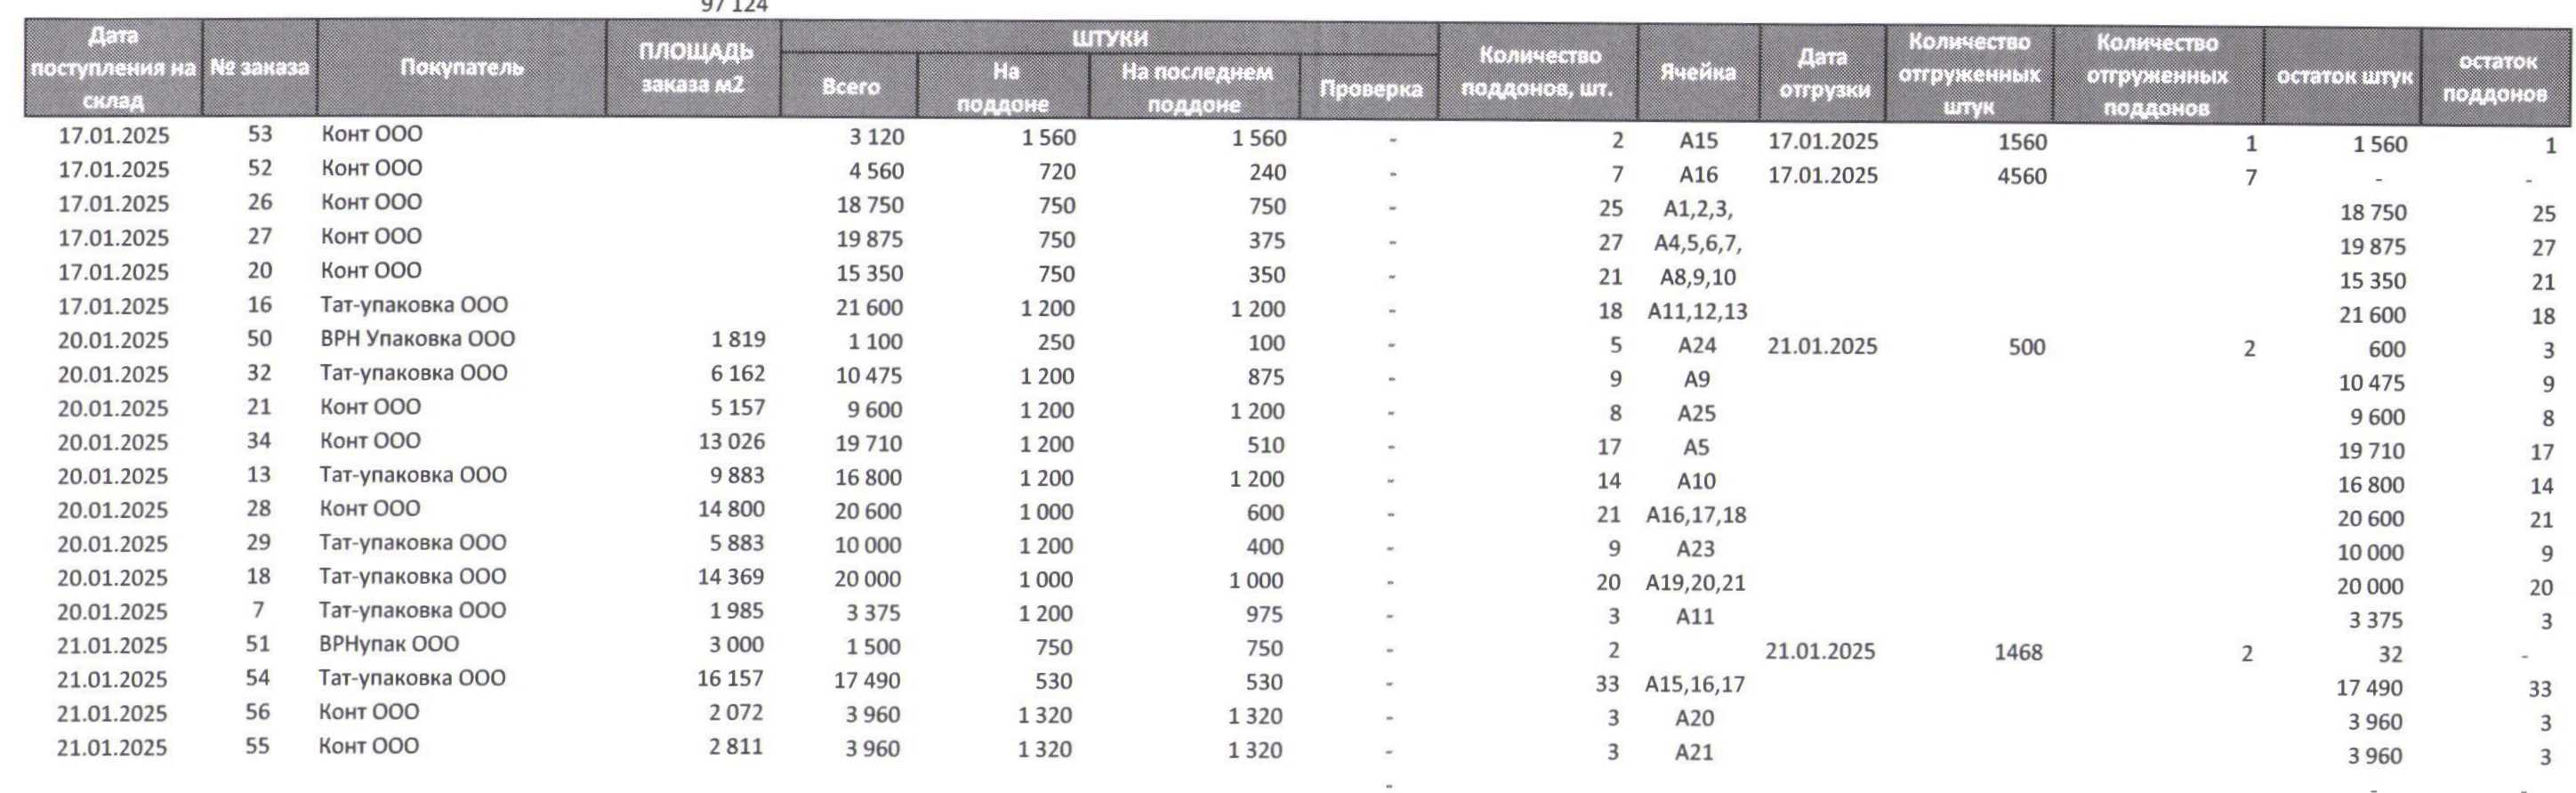
\includegraphics[width=\linewidth, height=0.94\textheight, angle=90, keepaspectratio]{Pics/f10.jpg}
\end{center}
\caption{Остатки готовой продукции на складе}
\label{pic:f10}
\end{figure}

\begin{figure}
\begin{center}
 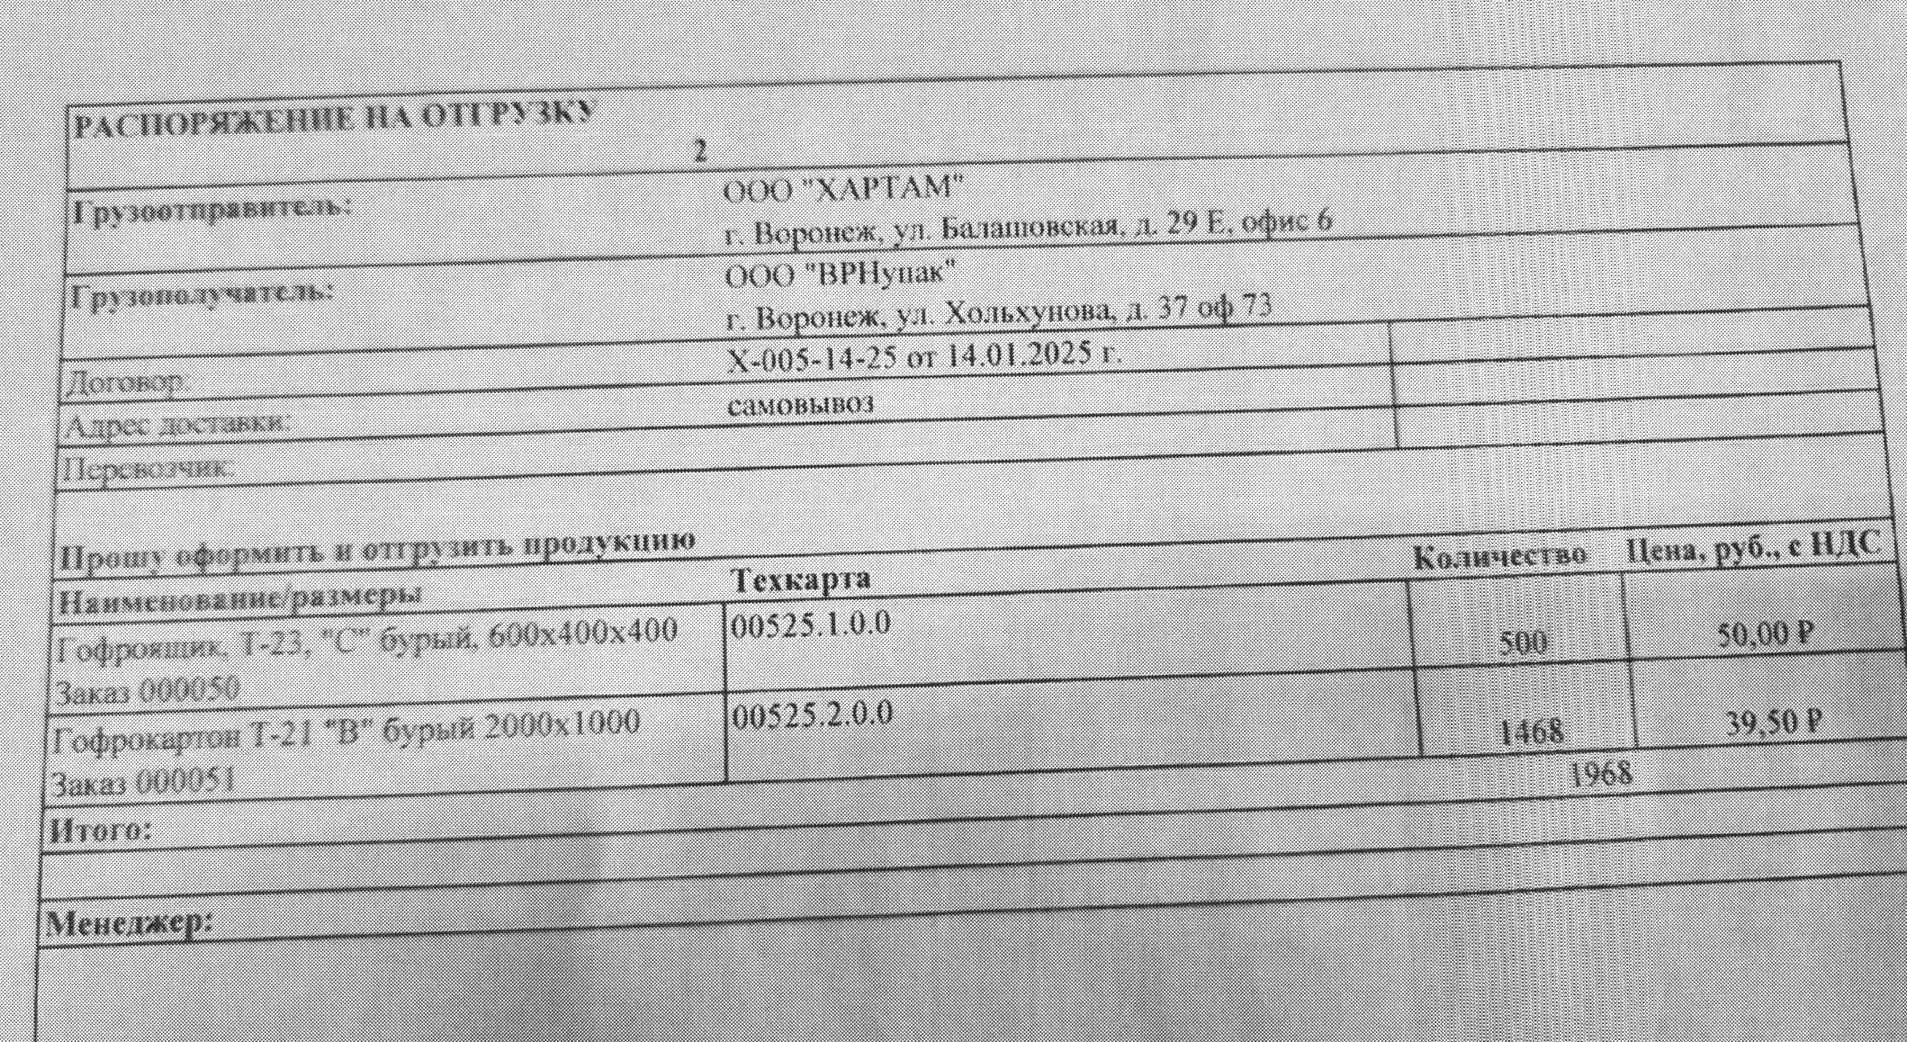
\includegraphics[width=\linewidth, height=0.94\textheight, keepaspectratio]{Pics/f11.jpg}
\end{center}
\caption{Распоряжение на отгрузку}
\label{pic:f11}
\end{figure}

\begin{figure}
\begin{center}
 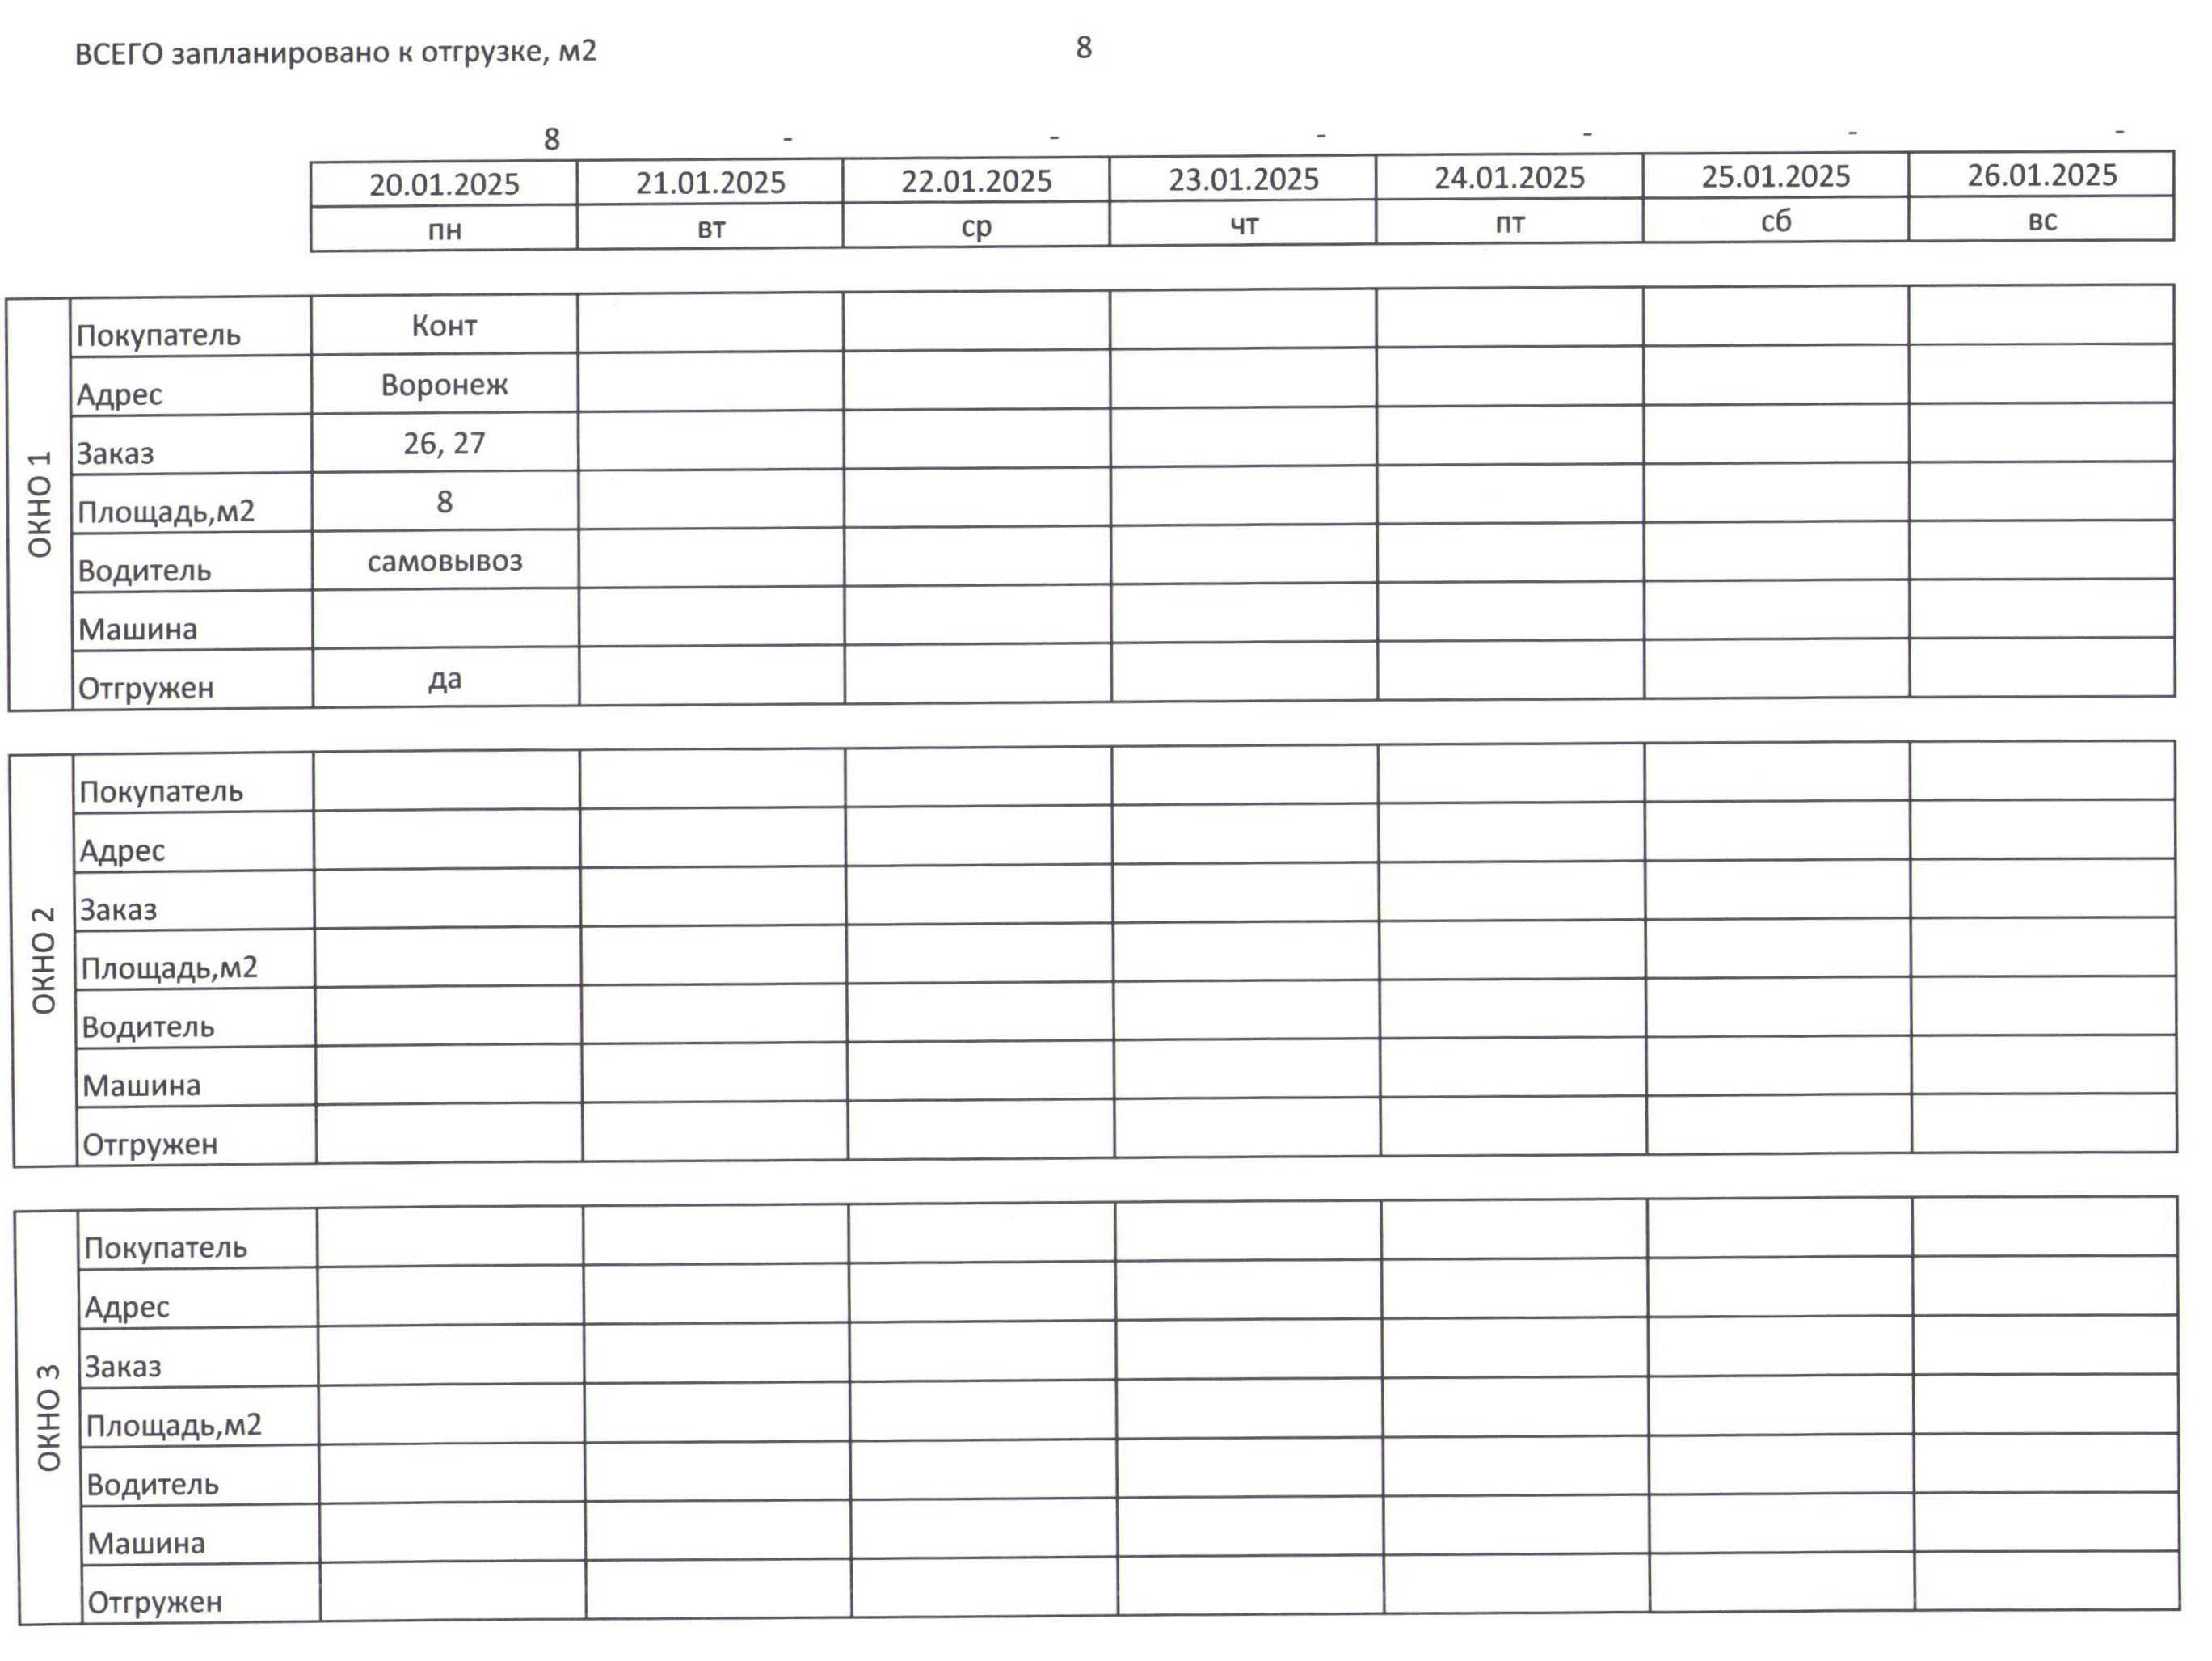
\includegraphics[width=\linewidth, height=0.94\textheight, keepaspectratio]{Pics/f14.jpg}
\end{center}
\caption{График отгрузки}
\label{pic:f14}
\end{figure}


\newpage
\subsection{Отгрузка готовой продукции}
\label{bp:Shipment}


Менеджер создает распоряжение на отгрузку и скидывает в общий чат в WhatsApp.  Начальник склада находит транспорт и сообщает данные об автомобиле. При отгрузке на условиях самовывоза менеджер сообщает в общем чате данные водителя, вид и номер транспортного средства. Кладовщик передает данные автомобиля на охрану. 

Графика подачи машин не выявлено, машины на погрузку подъезжают в любом порядке.
О прибытии транспорта на территорию предприятия охрана информирует склад. Кладовщик связывается с водителем и сообщает ему место погрузки. 

Кладовщик выполняет погрузку готовой продукции в транспорт: находит паллеты с готовой продукцией на складе согласно документу <<Распоряжение на отгрузку>>. 
Водитель погрузчика определяет место хранения готовой продукции на основе данных таблицы  данными таблицы MS EXCEL (рис. \ref{pic:f10}). 

Водитель погрузчика грузит продукцию в транспорт. Кладовщик фиксирует факт отгрузки в копии распоряжения на отгрузку.
После погрузки кладовщик в общем чате в WhatsApp сообщает о завершении погрузки, после чего бухгалтер формирует комплект сопроводительных документов, которые передает с водителем или пересылает заказчику по электронной почте.


На предприятии ведется реестр контрагентов с указанием используемого перечня отгрузочных документов (рис. \ref{pic:f12}). 


\begin{figure}
\begin{center}
 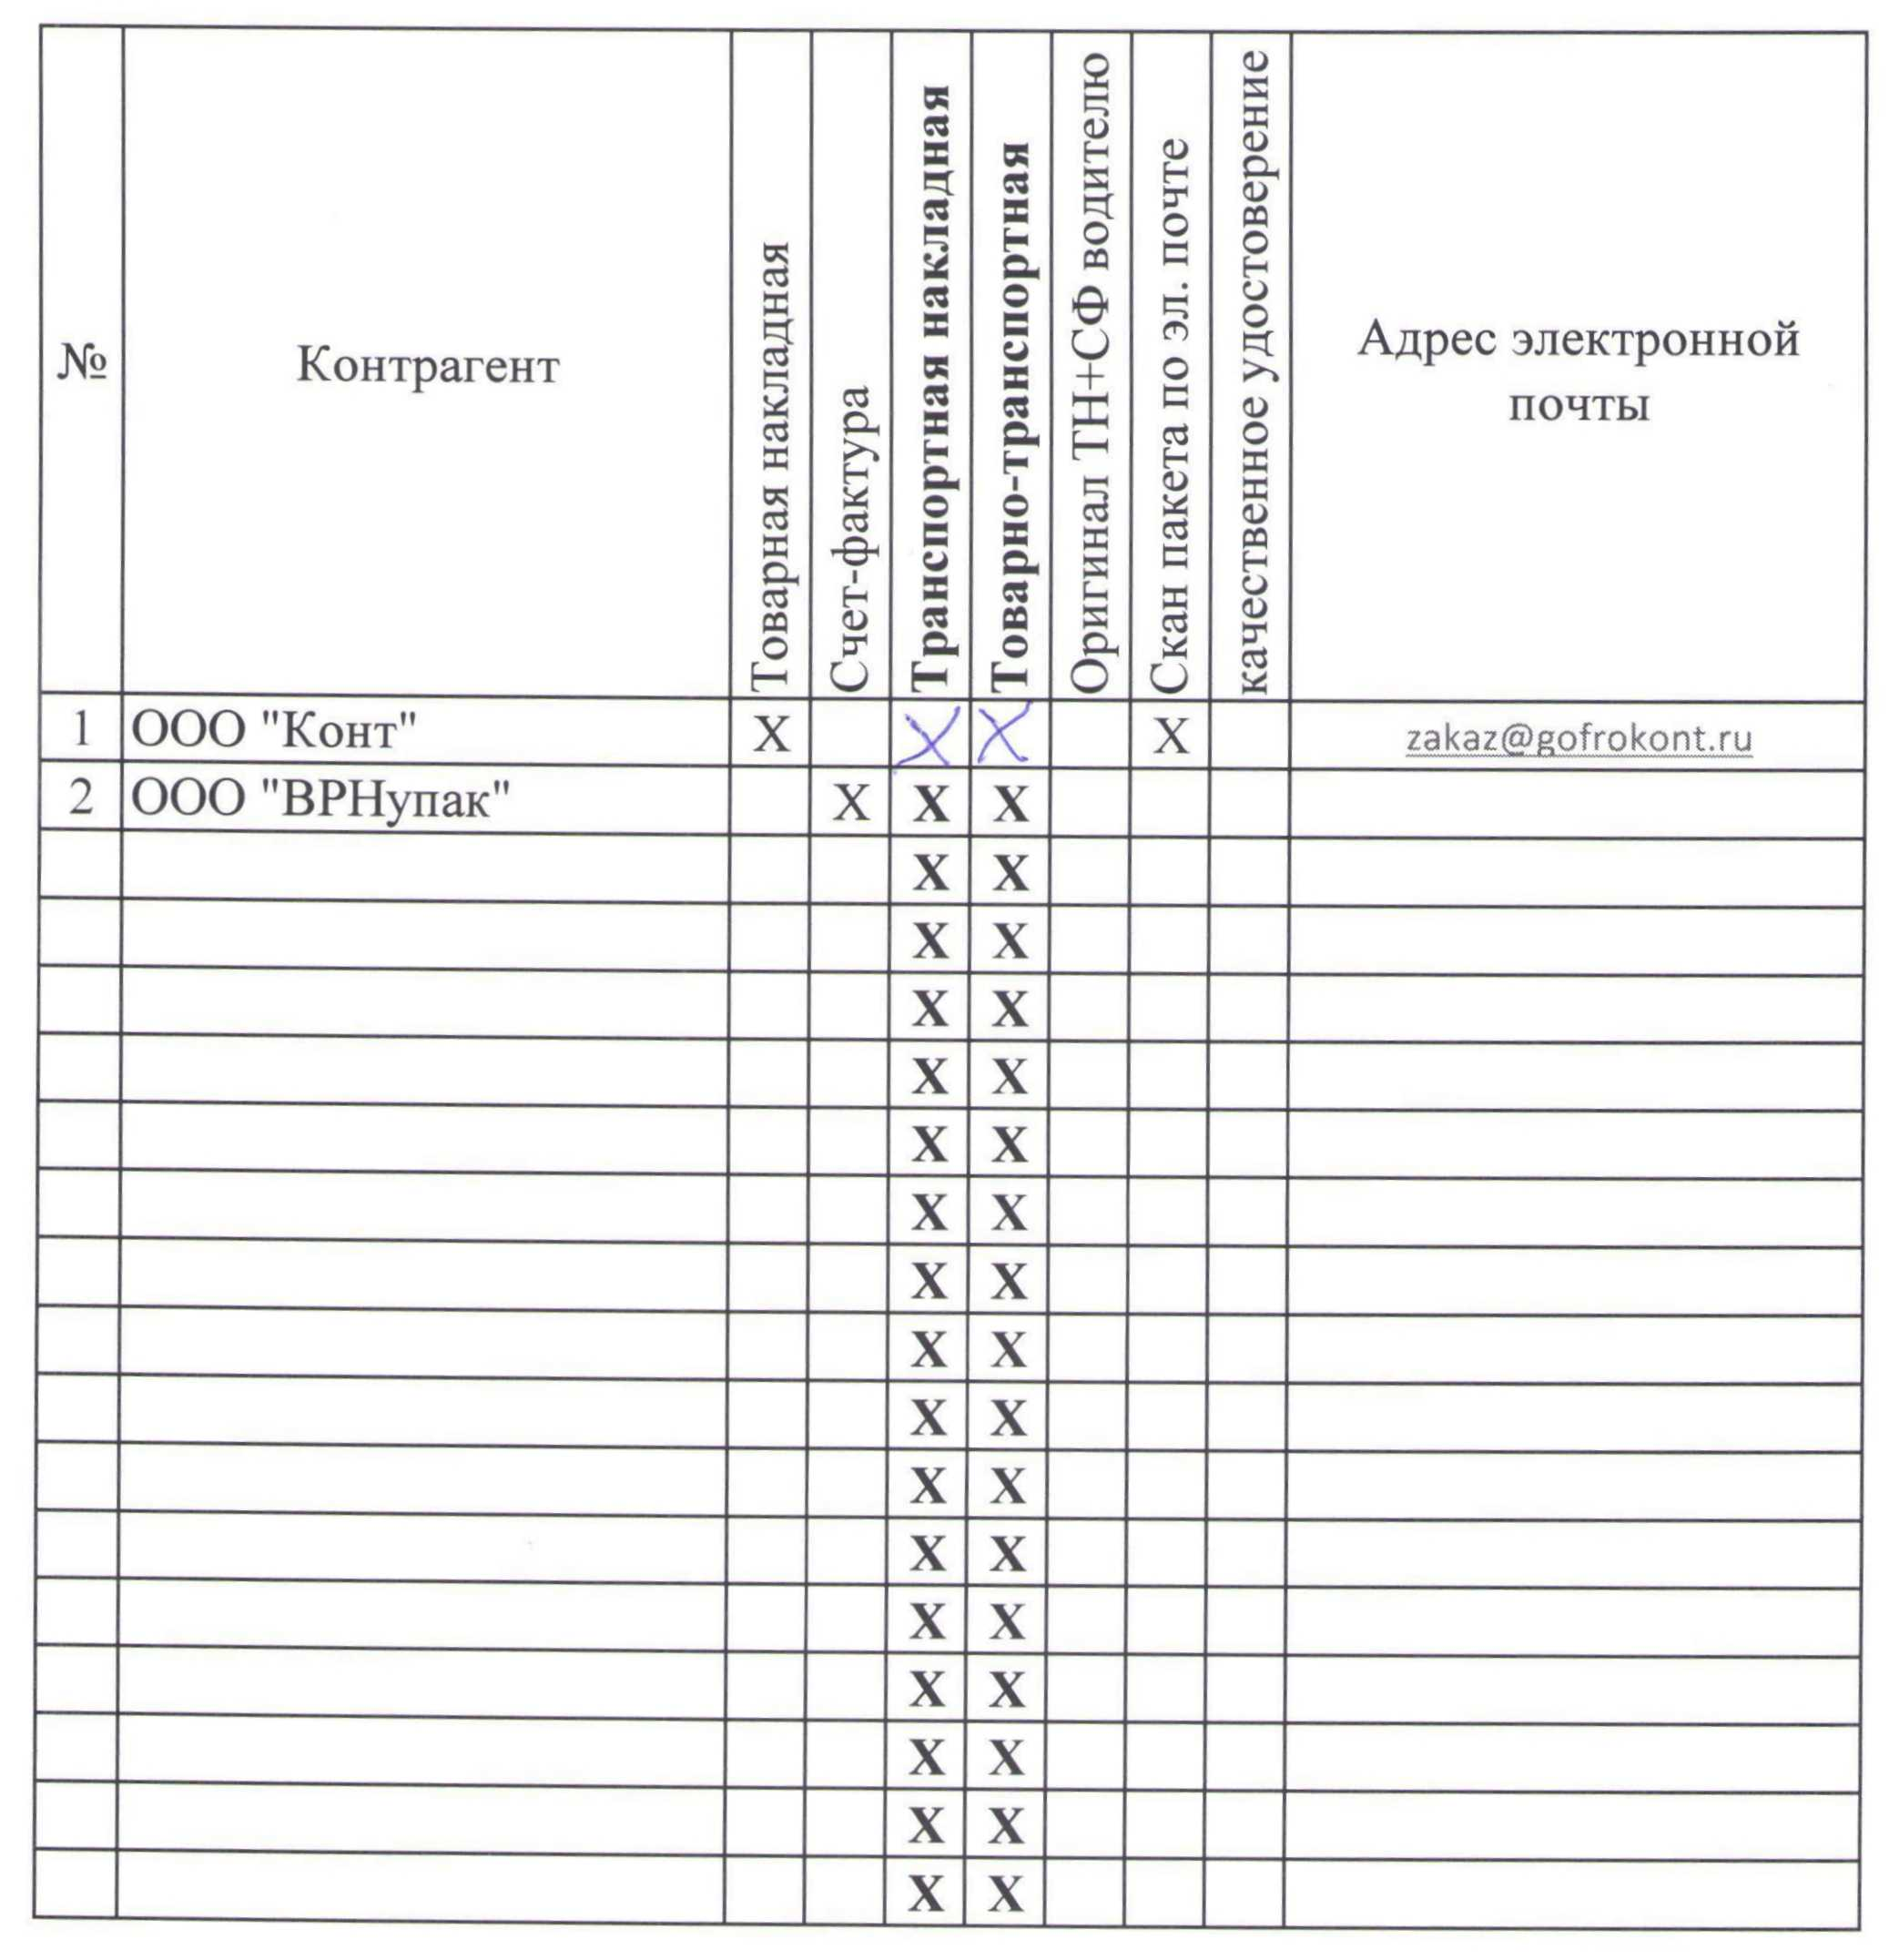
\includegraphics[width=\linewidth, height=0.94\textheight, keepaspectratio]{Pics/f12.jpg}
\end{center}
\caption{Реестр контрагентов}
\label{pic:f12}
\end{figure}

\clearpage
\newpage
\subsection{Планирование сырья}
\label{bp:RawMaterialPlanning}

\textbf{Планирование бумаги и картона}

Планирование основного сырья (бумага и картон) выполняется главным технологом. 

Нормативы по сырью на момент проведения аудита не разработаны. 

Основное сырье (бумага и картон) поставляется предприятием ООО ''Эколайнер''.


% \textbf{Планирование закупки заготовок}


% % \todo{перечитать с планированием}



\textbf{Планирование вспомогательных материалов}

На момент проведения аудита не регламентировано.

% Планированием и закупкой вспомогательных материалов занимается отдел снабжения.

% Каждый день техник по учету определяет остатки по крахмалу и другим материалам (Пленка, скотч и др.) в производстве и сообщает по телефону в отдел снабжения остатки на складе. 25 числа каждого месяца менеджер по снабжению заказывает поставки крахмала на следующий месяц. Объемы заказа определяются коллективно с техником по учету. Менеджер отдела снабжения обзванивает поставщиков по ценам, формирует заявку в свободной форме. Поставки крахмала выполняются 2-3 раза в месяц.

% В системе СБИС хранятся текущие остатки на складах, но отдел снабжения не использует систему СБИС.


% По закупке других материалов (СИЗ, спецодежда, комплектующие и запчасти) отдел снабжения собирает заявки от подразделений, обрабатывает их, ищет поставщиков и производит закупку.


% Поддоны.

% Начальник склада каждый вечер определяет потребность по поддонам и сообщает по телефону в отдел снабжения, где менеджеры отдела снабжения фиксирует вручную объемы потребности.
% Коммерческий отдел и отдел снабжения совместно определяют потребность в поддонах исходя из плана производства и текущих остатков на складах и заказывают поддоны у производителей.
% Менеджеры отдела снабжения создают заявку на закупку поддонов и спецподдонов. Все поддоны невозвратные.
% Поддоны принимаются на складе. Учет поступления фиксируется в системе СБИС.


\textbf{Планирование краски }

На момент проведения аудита не регламентировано.





\clearpage
\ifx \notincludehead\undefined
\normalsize
\end{document}
\fi
%\newpage
\subsection{Оперативное планирование производства}
\label{bp:OperPlan}


Все заявки от покупателей менеджер отдела продаж регистрирует в таблице MS EXCEL.




\textbf{Планирование работы гофроагрегата}

Главный технолог используя шаблон в таблице MS EXCEL кроит (осуществляет поиск подкроя по ширине гофрополотна на гофроагрегате)  задания на гофроагрегат вручную. 

Утверждено несколько марок выпускаемого картона. Композитный состав не утвержден.



\textbf{Планирование линий переработки}

Главный технолог создает план на переработку вручную по каждой производственной линии в таблице MS EXCEL %\ref{pic:d4}.

Главный технолог печатает задание на линию и передает мастеру производства. 
Мастер производства при получении плана работы самостоятельно распределяет задания по линиям исходя из загруженности производственных мощностей.
Задания передаются операторам линий переработки. 



\clearpage

\ifx \notincludehead\undefined
\normalsize
\end{document}
\fi
%\newpage
\subsection{Подготовка производства}
\label{bp:Prepare}
%

Единая форма для сбора входящей информации (опросный лист) отсутствует.
Заказчик присылает требования на изготовления продукции в произвольной форме.

Обработка запроса может производиться на основании образец продукции, предоставленного заказчиком. Полученный от заказчика образец изделия из гофрокартона передается дизайнеру, который производит измерение размеров. Дизайнер производит расчет размеров требуемого изделия из гофрокартона в случае, если заказчик в качестве образца передал упаковываемый товар.

От менеджера дизайнерам поступает заявка (рис. \ref{pic:f16}), где прописываются требования к изделиям. 

Дизайнер переносит данные вручную в шаблон ТК, разработанный в MS EXCEL. Часть данных просчитывается по формуле. Параметры без формул  рассчитываются вручную. Технологическая карта разрабатывается в виде таблицы в MS EXCEL (рис. \ref{pic:f15}).

При разработке технологической карты для изделия, производимого с использованием штампа, менеджер передает в отдел дизайна макет штампа. 
После обработки макет отправляется главному технологу. Главный технолог чертит принимает решение о количестве мест на штампе и информацию передает в виде карандашного рисунка, сделанного своей рукой.
Главный технолог разрабатывает маршрут изготовления ГП. 
После внесения корректировок в ТК, производимых главным технологом, ТК возвращается дизайнерам. Далее дизайнеры отсылают готовый макетом поставщику штампов, размещают заказ на изготовление.

При разработке дизайна менеджер передает дизайнерам эскиз печати. Этот эскиз обрабатывают и передают поставщику клише для изготовления оснастки. 

После создания технологической карты дизайнер отправляет ее на согласование главному технологу. Только после согласования главным технологом ТК направляют менеджеру отдела продаж для утверждения заказчиком. 
  
При необходимости выкрасов дизайнер совместно с колористом определяют номер оттенка по шкале Pantone. Номер кода цвета отсылают в Москву в компанию <<АГ Флекс>>, откуда приходит формула цвета, по которой смешивают краску и делают выкрасы вручную.

Номер технологической карты присваивают дизайнеры.


Готовые технологические карты хранят на сервере в виде таблиц MS EXCEL. К ним имеют доступ все заинтересованные лица без возможности внесения изменений.

При внесении в уже действующую технологическую карту изменений дизайнеры создают новую ТК, которой присваивается новый номер.


\begin{figure}
\begin{center}
 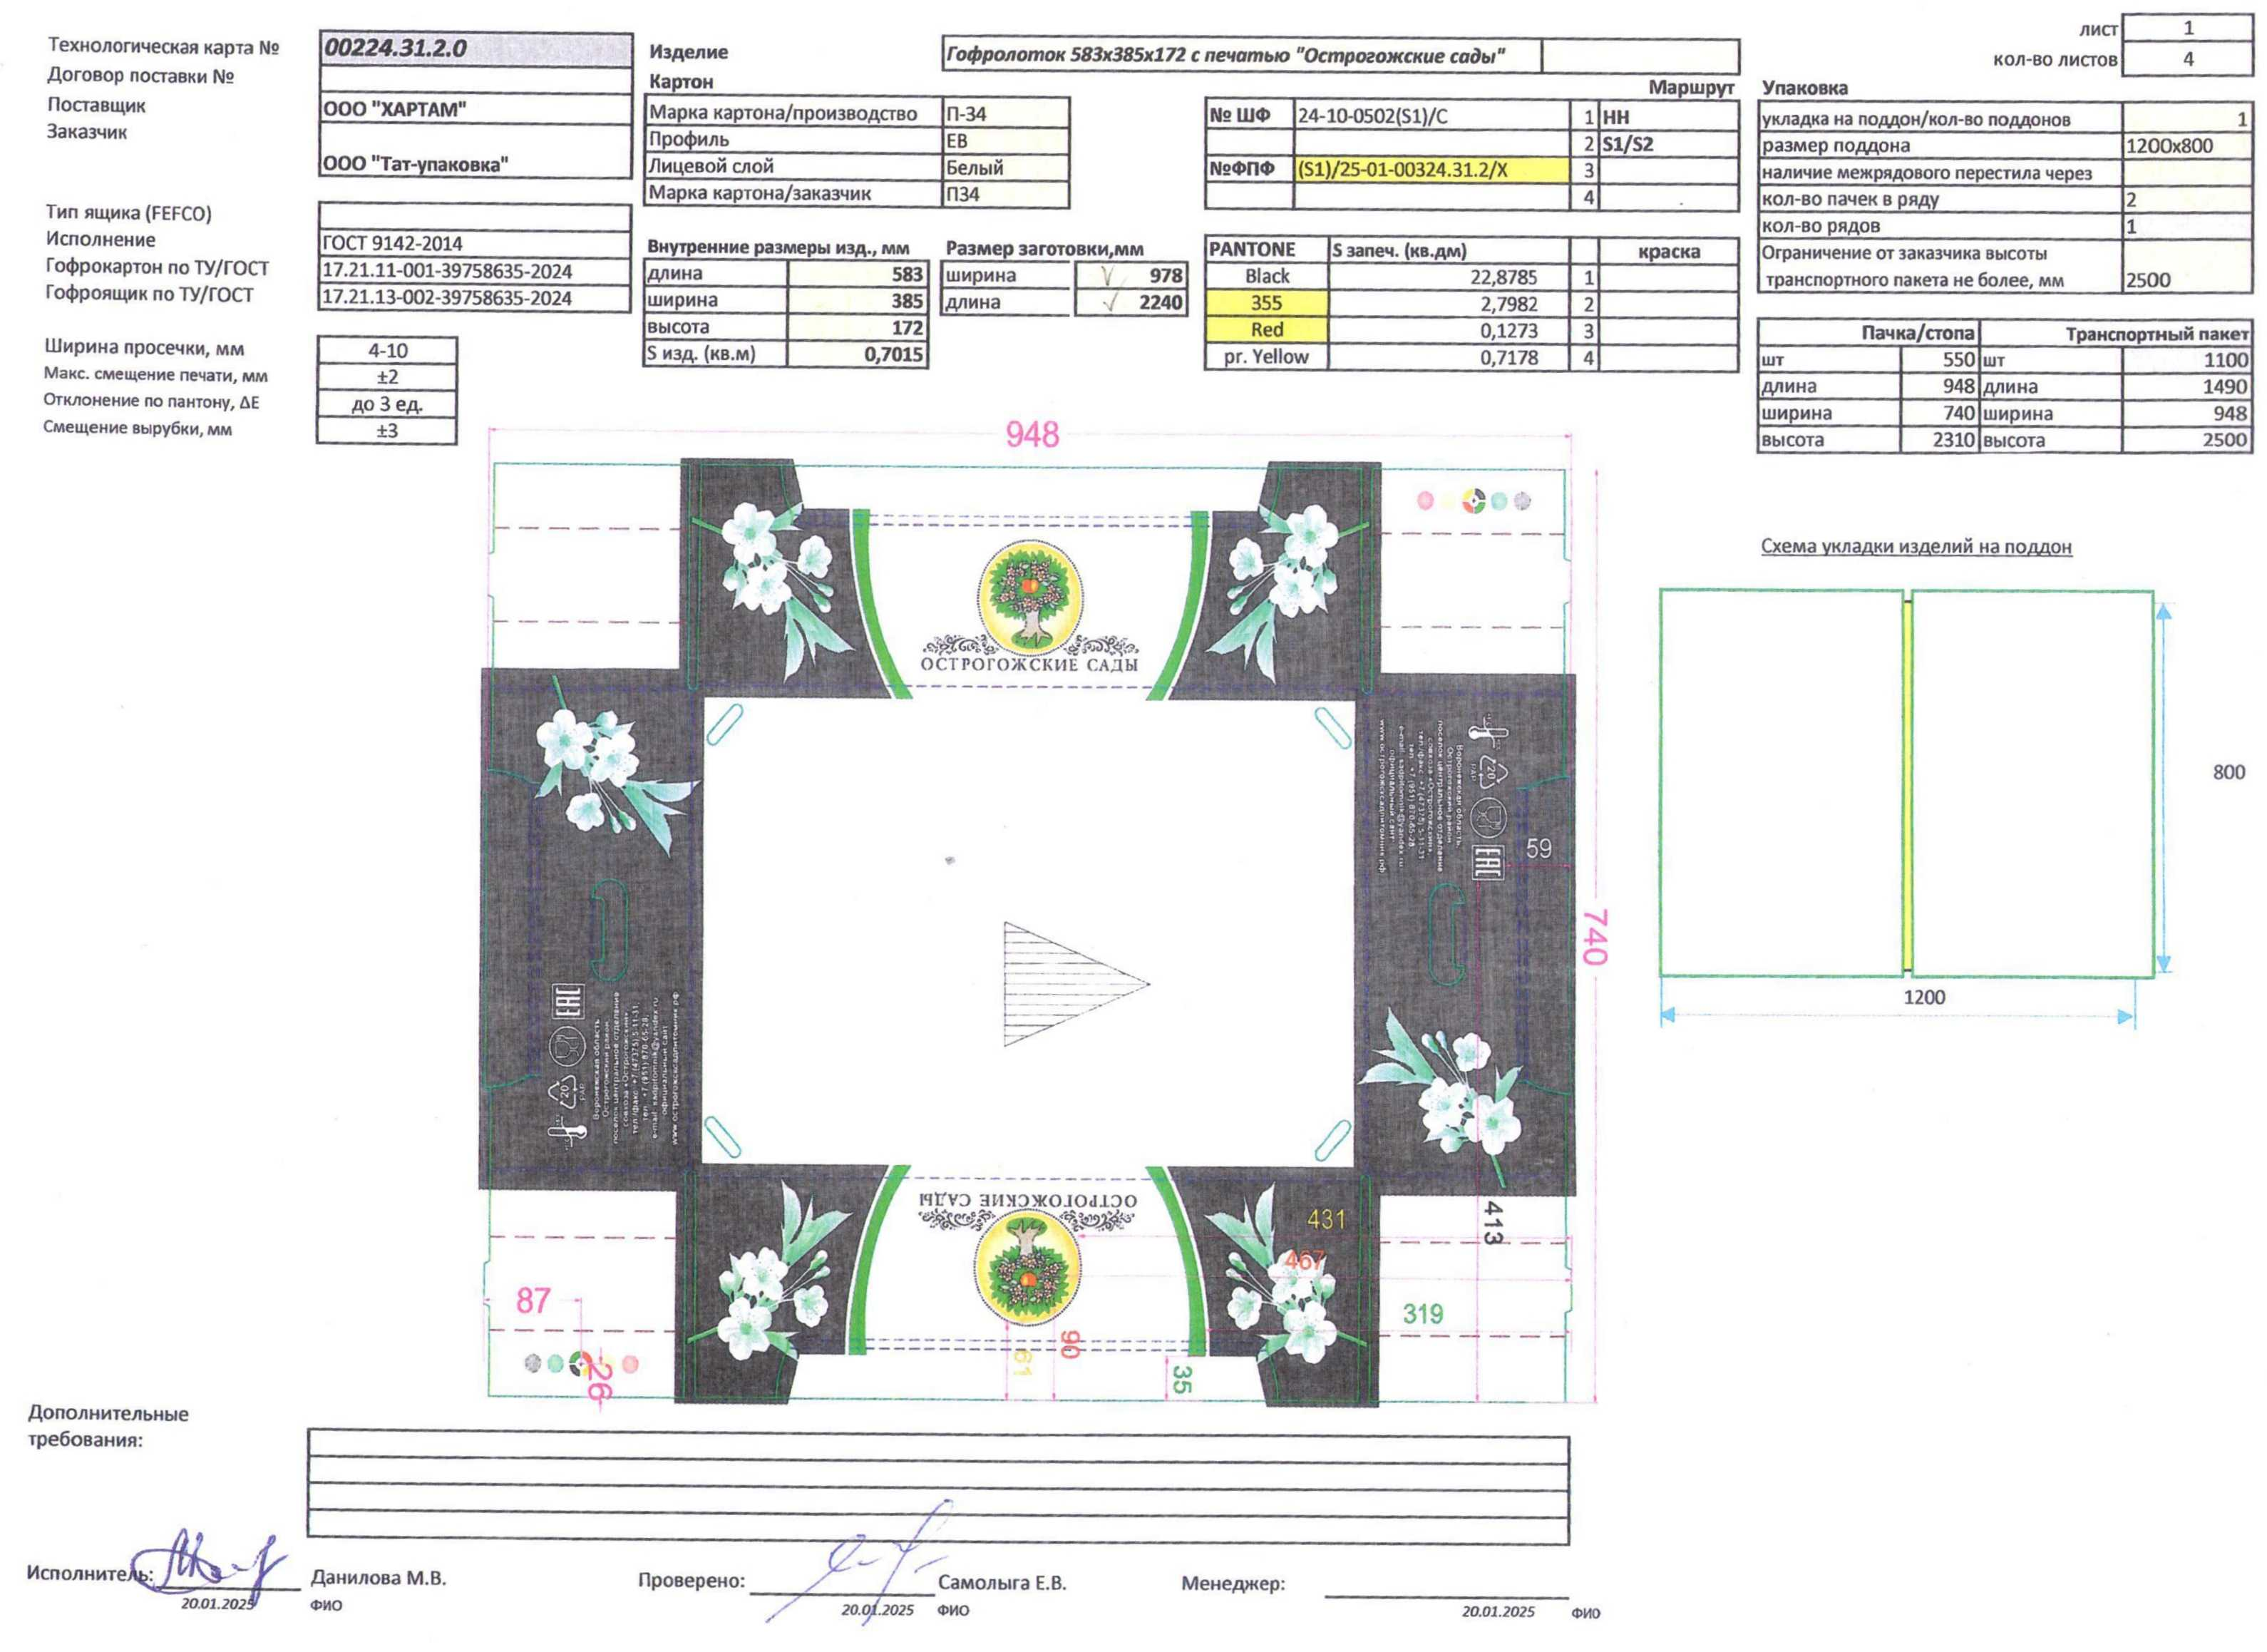
\includegraphics[width=\linewidth, height=0.94\textheight, angle=90, keepaspectratio]{Pics/f15.jpg}
\end{center}
\caption{Разработка ТК}
\label{pic:f15}
\end{figure}

\begin{figure}
\begin{center}
 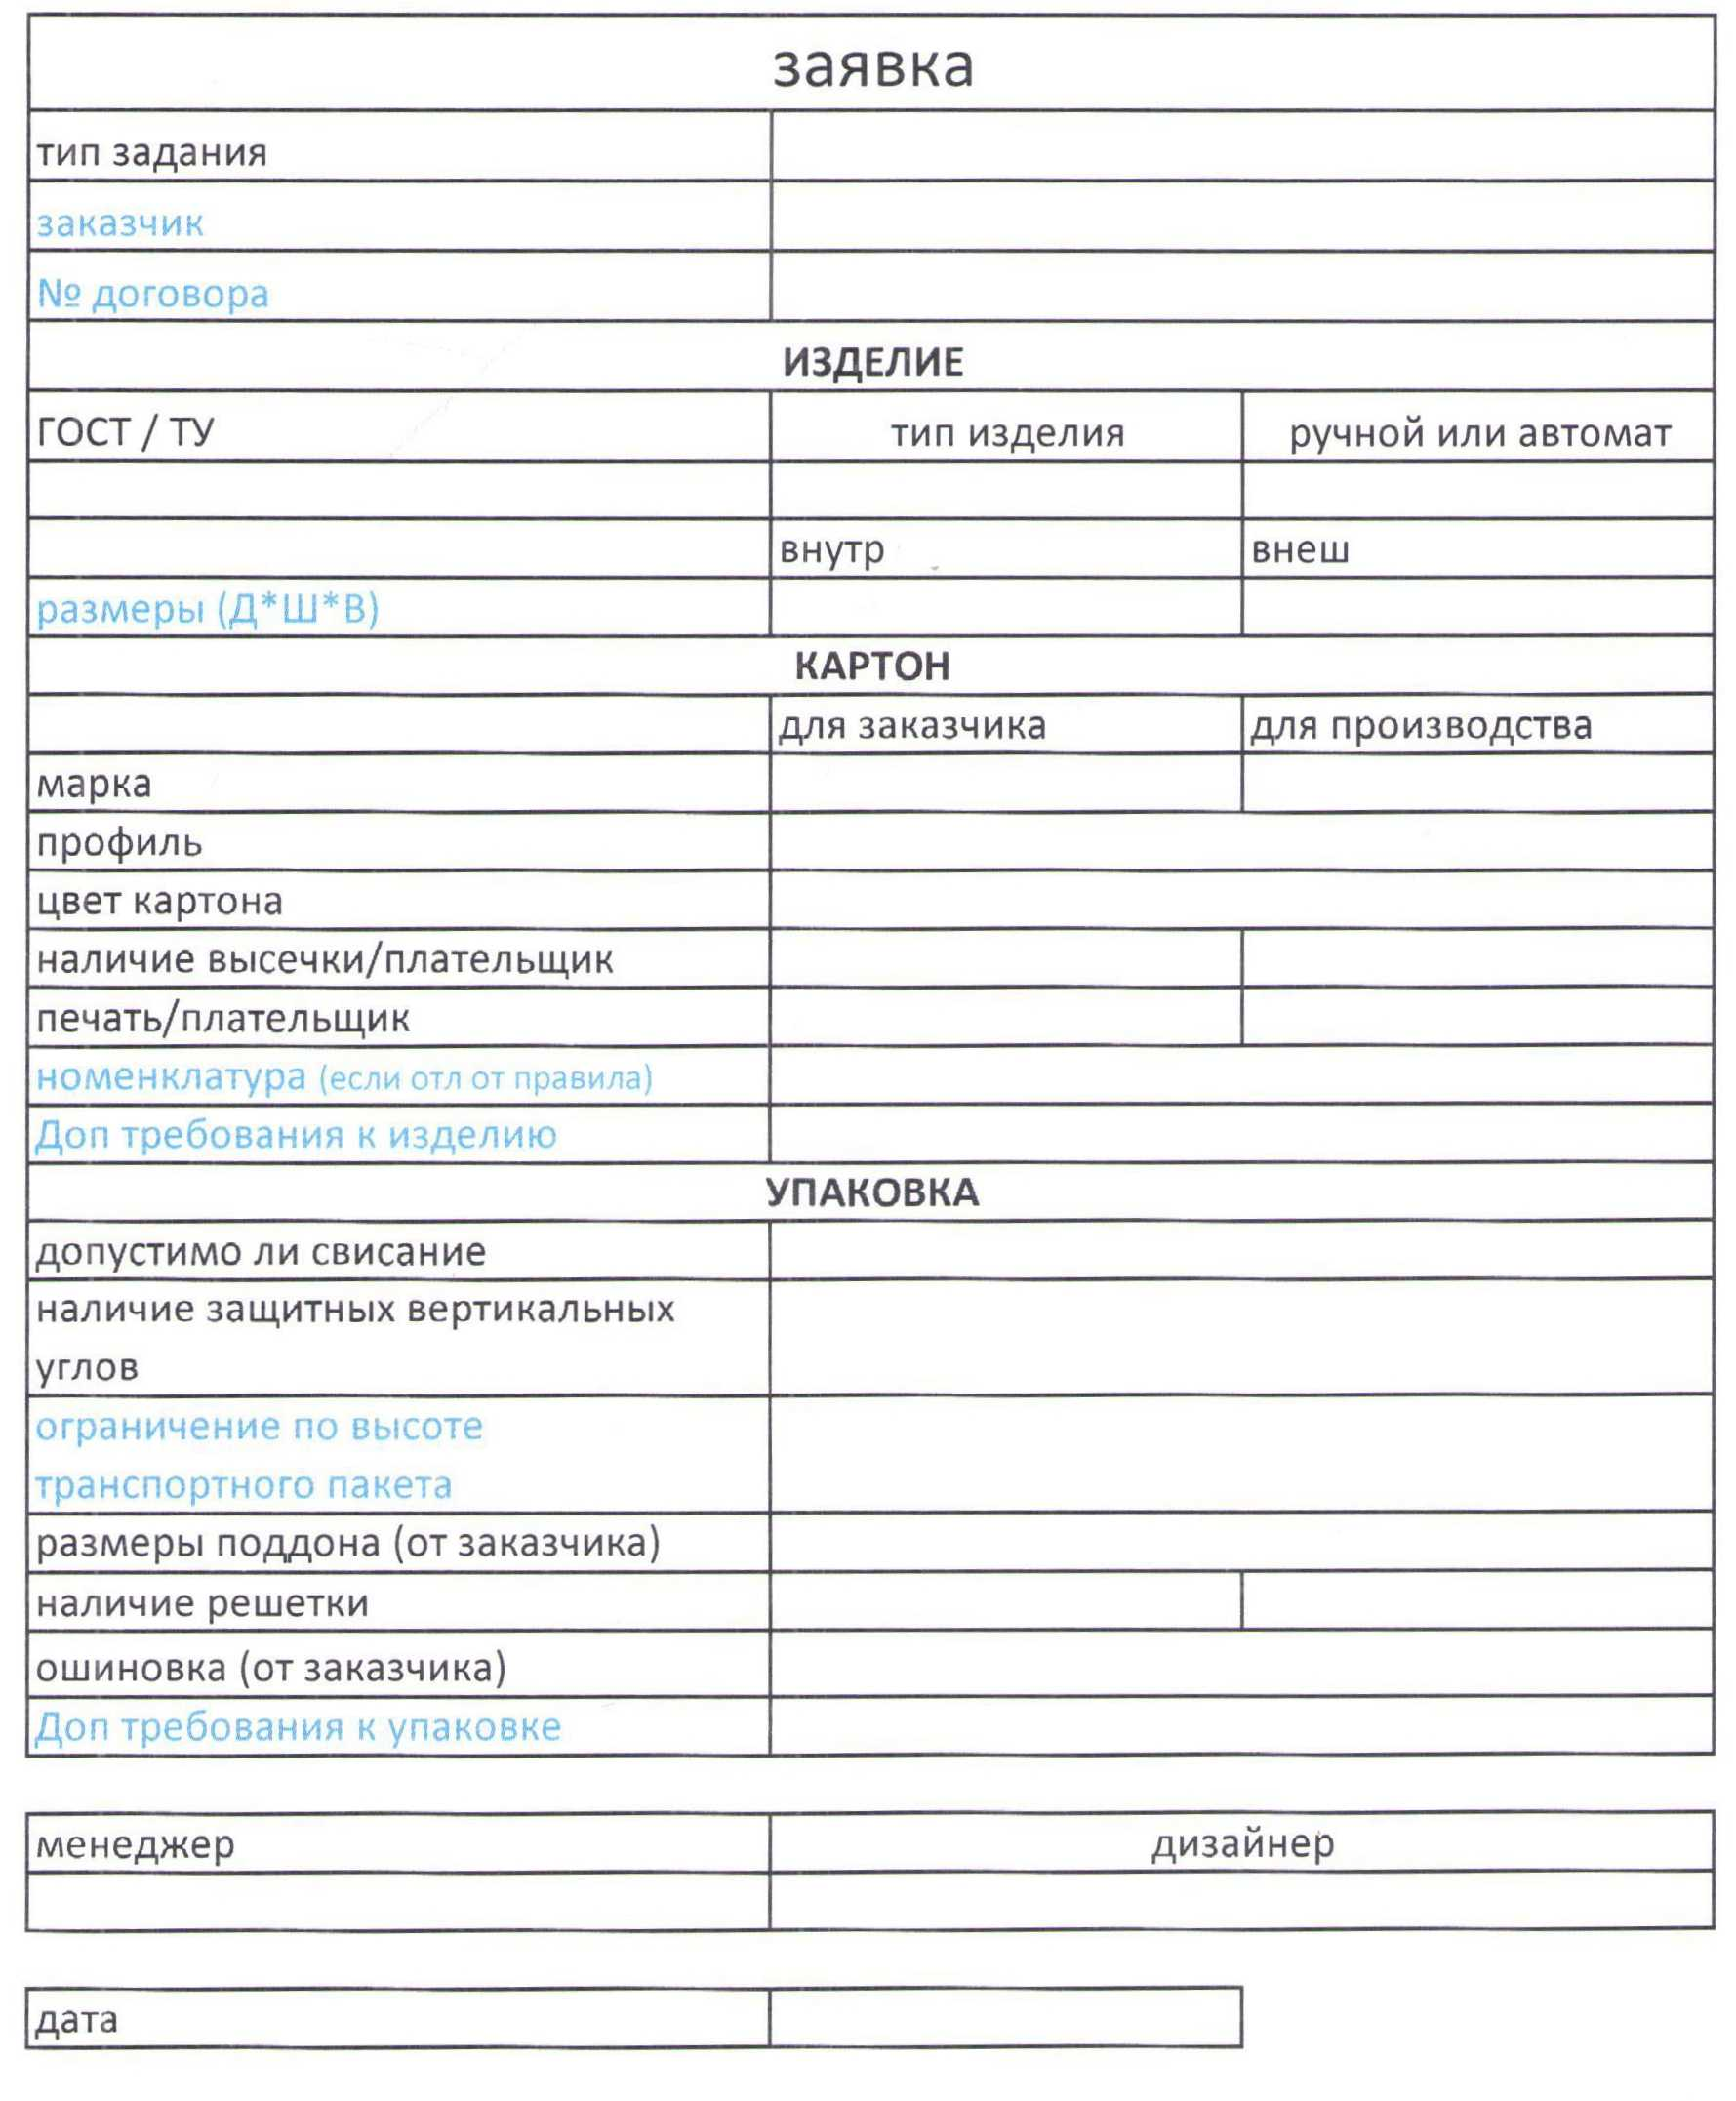
\includegraphics[width=\linewidth, height=0.94\textheight, keepaspectratio]{Pics/f16.jpg}
\end{center}
\caption{Заявке на разработку чертежа и макета}
\label{pic:f16}
\end{figure}
%\end{figure}


\clearpage
\ifx \notincludehead\undefined
\normalsize
\end{document}
\fi
\newpage
\subsection{Учет технологической оснастки и краски }
\label{bp:rigging}
%
Технологическая оснастка необходима для изготовления готовой продукции. На предприятии заказывают оснастку у сторонних производителей.

При получении требований от клиента менеджер определяет необходимость использования оснастки при производстве продукции. 

Возможность изготовления нового изделия, в соответствии с техническими параметрами оборудования, определяет главный технолог. 




\textbf{Учет клише}

Дизайнер, на основании разработанного и согласованного дизайна заказывает изготовление клише. 

Предприятие использует одного поставщика клише. 
Для размещения заказа на изготовление клише дизайнер отправляет макет по электронной почте.

Учет количества размещенных заявок на изготовление клише не ведется. 
При изготовлении клише за счет клиента менеджер создает запрос в бухгалтерию для выставления счета. Бухгалтер выставляет счет на изготовление оснастки.

При поступлении на производство клише проверяется на соответствие макету, фиксируется дата поступления в MS EXCEL (рис. \ref{pic:f17}). Кладовщики о факте поступлении оснастки сообщают дизайнерам. 

Номер клише присваивает дизайнеры в момент заказа у поставщика.

На предприятии выделен участок для хранения клише.


\textbf{Учет штанцевальных форм}

 Менеджер передает в отдел дизайна макет штампа. Далее данный макет обрабатывается и отсылается главному технологу. Главный технолог чертит раскладку на штампе и прописывает оборудование, возвращает дизайнерам. Далее дизайнеры отсылают раскладку с макетом поставщику штампов и заказываю штамп.

Компания-изготовитель оснастки выставляет счет. Если изготовление штанцевальной формы выполняется за счет клиента, то менеджер делает запрос в бухгалтерию на выставление счета. Бухгалтер выставляет счет покупателю.

При поступлении штампа на производство  штамп проверяется. 

Номер присваивают дизайнера в момент заказа.

На предприятии места для хранения штампов оборудованы рядом с перерабатывающими линиями. Предусмотрена ячеистая система хранения. 

Учет штанцевальных форм ведется MS EXCEL, где указывается номер штампа и номер ячейки хранения (рис. \ref{pic:f22}).

Ремонтом оснастки занимаются в основном на производстве. Учет объема выполненных ремонтных работ не ведется.


Журнала выдачи оснастки не обнаружено.




%\subsubsection{Учет печатных форм}




%\subsubsection{Изготовление штампов}




\textbf{Учет краски}

Колорист получает задание на смену для каждой отдельной линии (рис. \ref{pic:f18}), подбирает технологические карты, по которым определяет номера краски, планируемой в работу. Колорист <<по своему опыту>> готовит краску на заказ (рецептура используется номинально). 

После приготовления краску выдают на линию. Учет краски колорист ведет в MS EXCEL (рис. \ref{pic:f19} - рис. \ref{pic:f20}). Общий итог расхода определяется по таблице MS EXCEL (рис. \ref{pic:f21}).

\begin{figure}
\begin{center}
 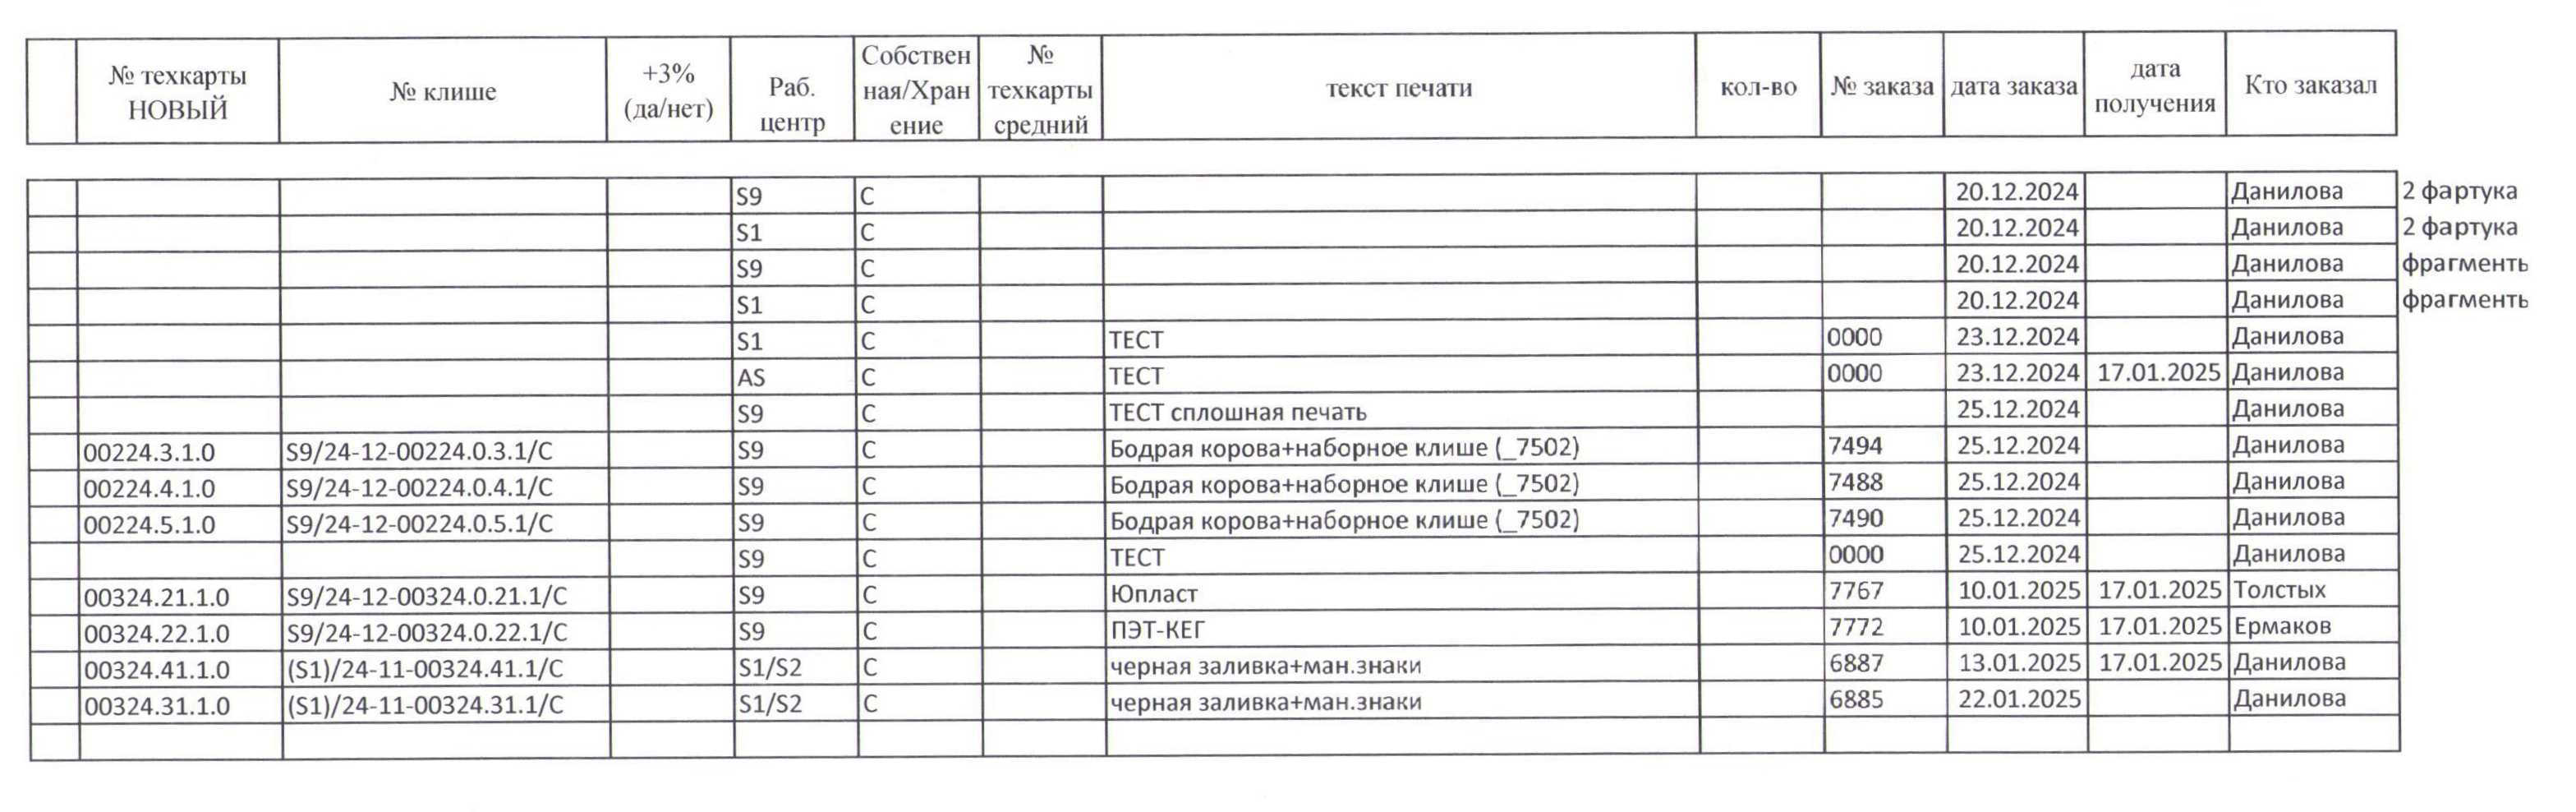
\includegraphics[width=\linewidth, height=0.94\textheight, angle=90, keepaspectratio]{Pics/f17.jpg}
\end{center}
\caption{Электронный реестр клише}
\label{pic:f17}
\end{figure}

\begin{figure}
\begin{center}
 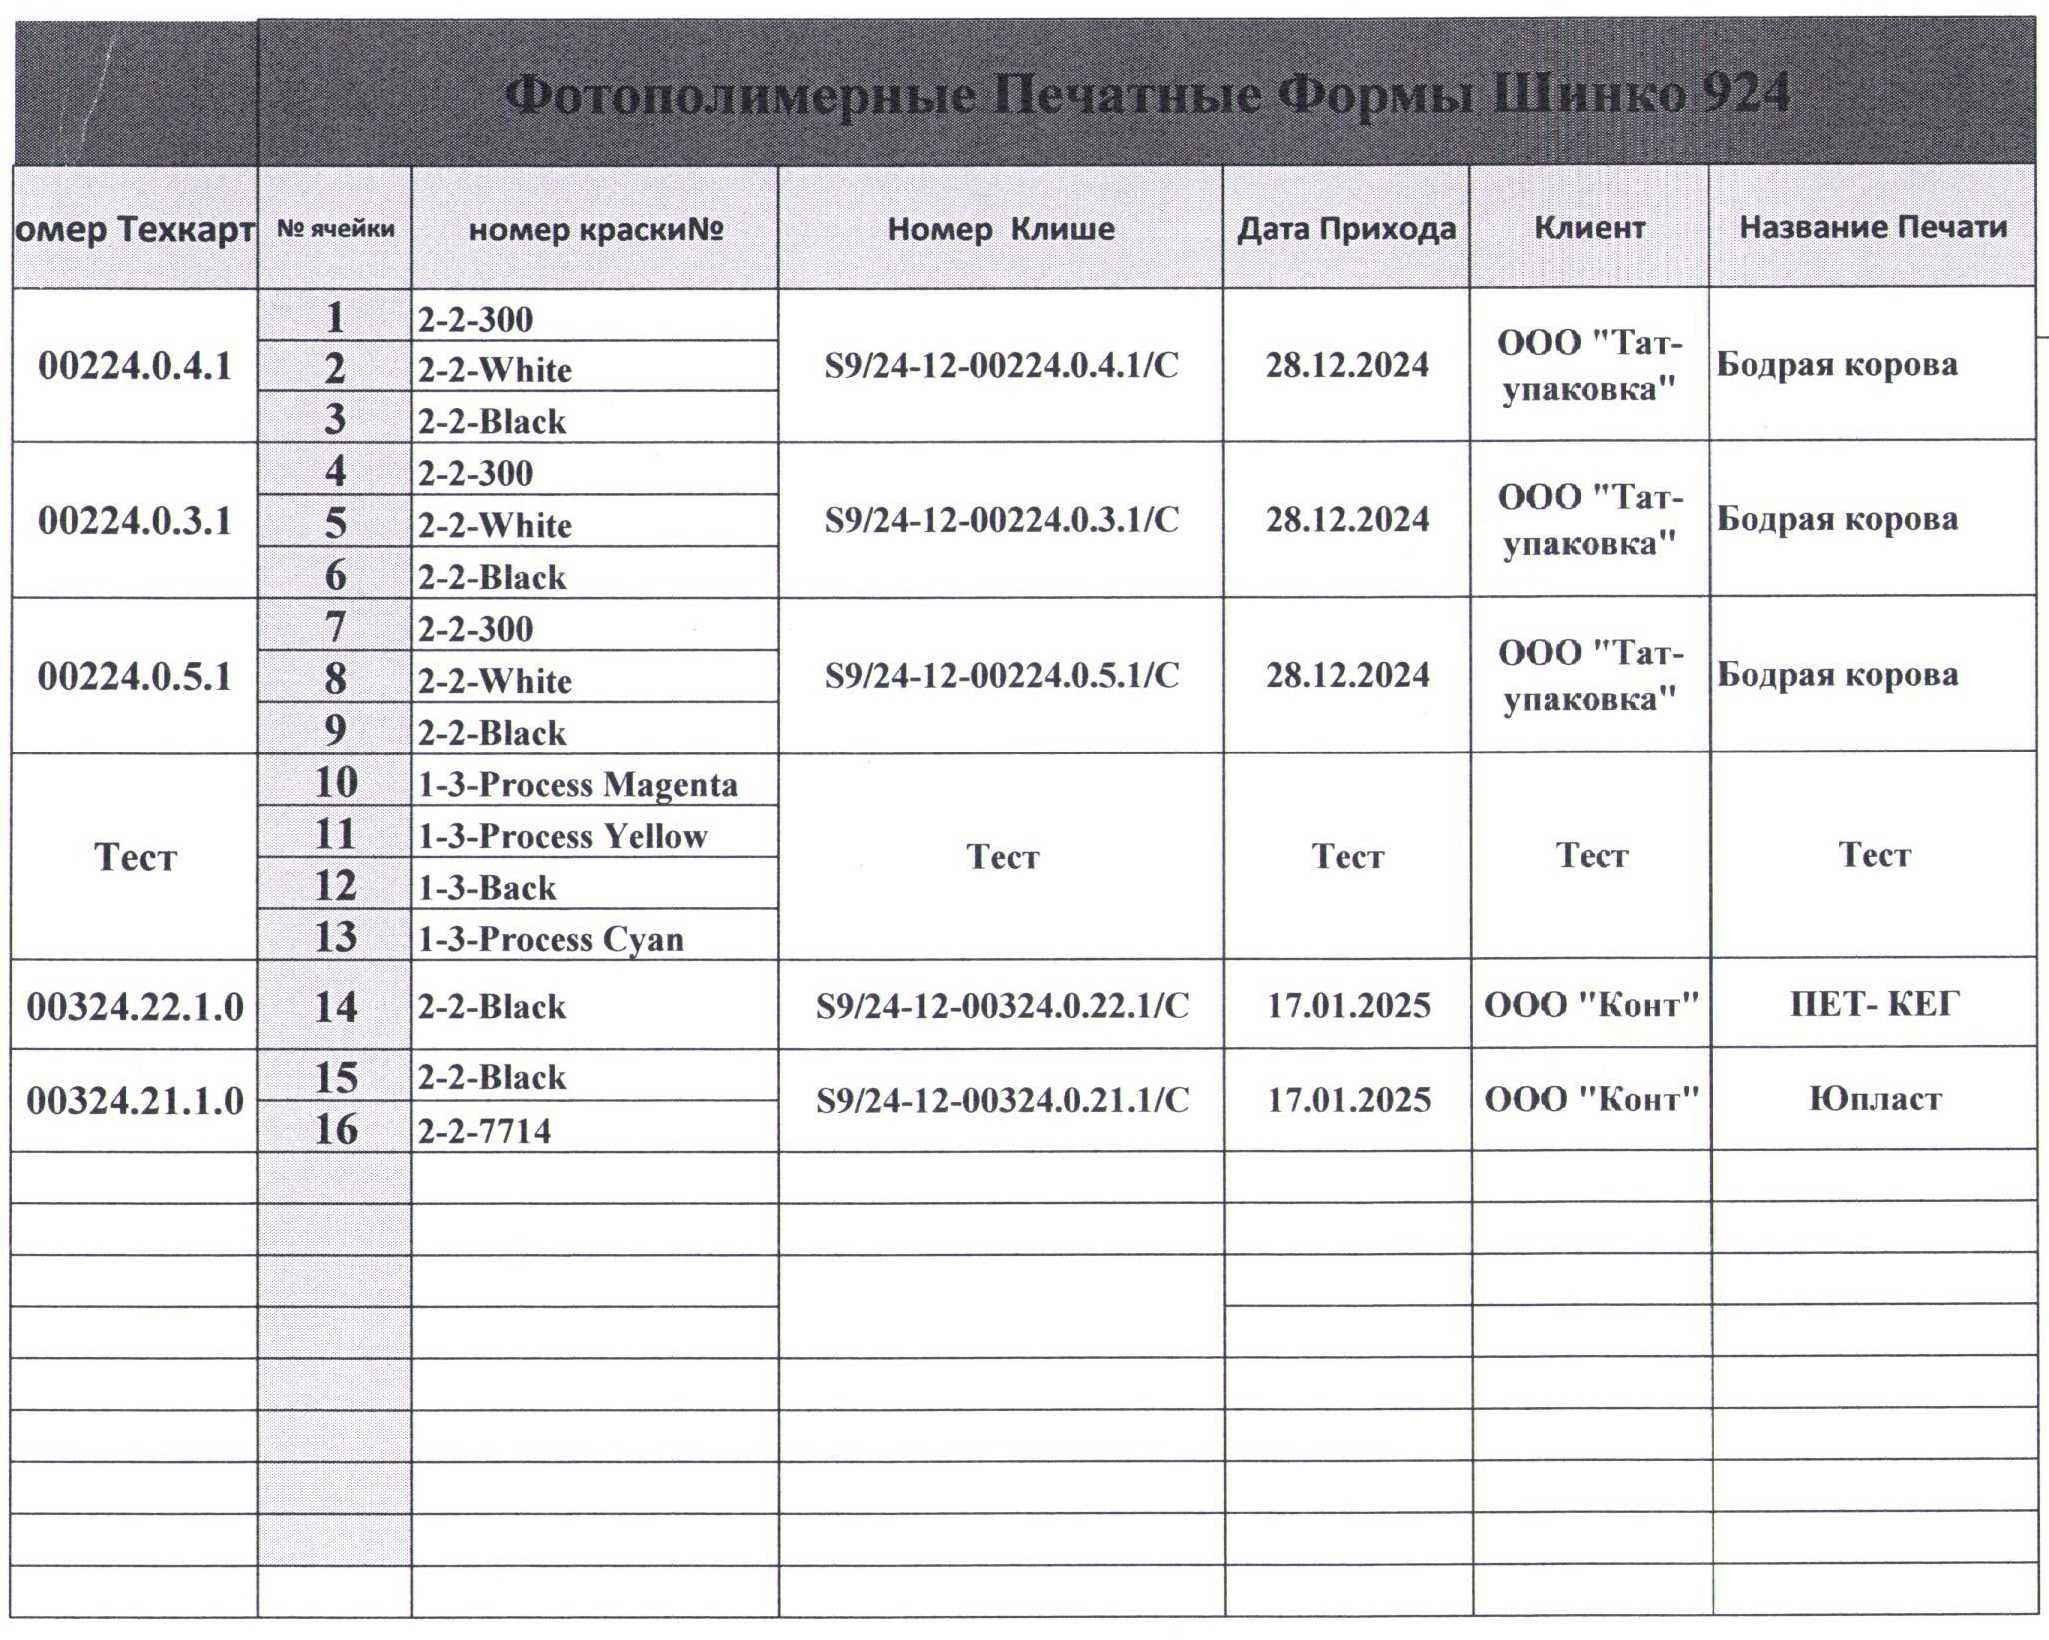
\includegraphics[width=\linewidth, height=0.94\textheight, keepaspectratio]{Pics/f22.jpg}
\end{center}
\caption{Каталог размещения клише в ячейках}
\label{pic:f22}
\end{figure}

\begin{figure}
\begin{center}
 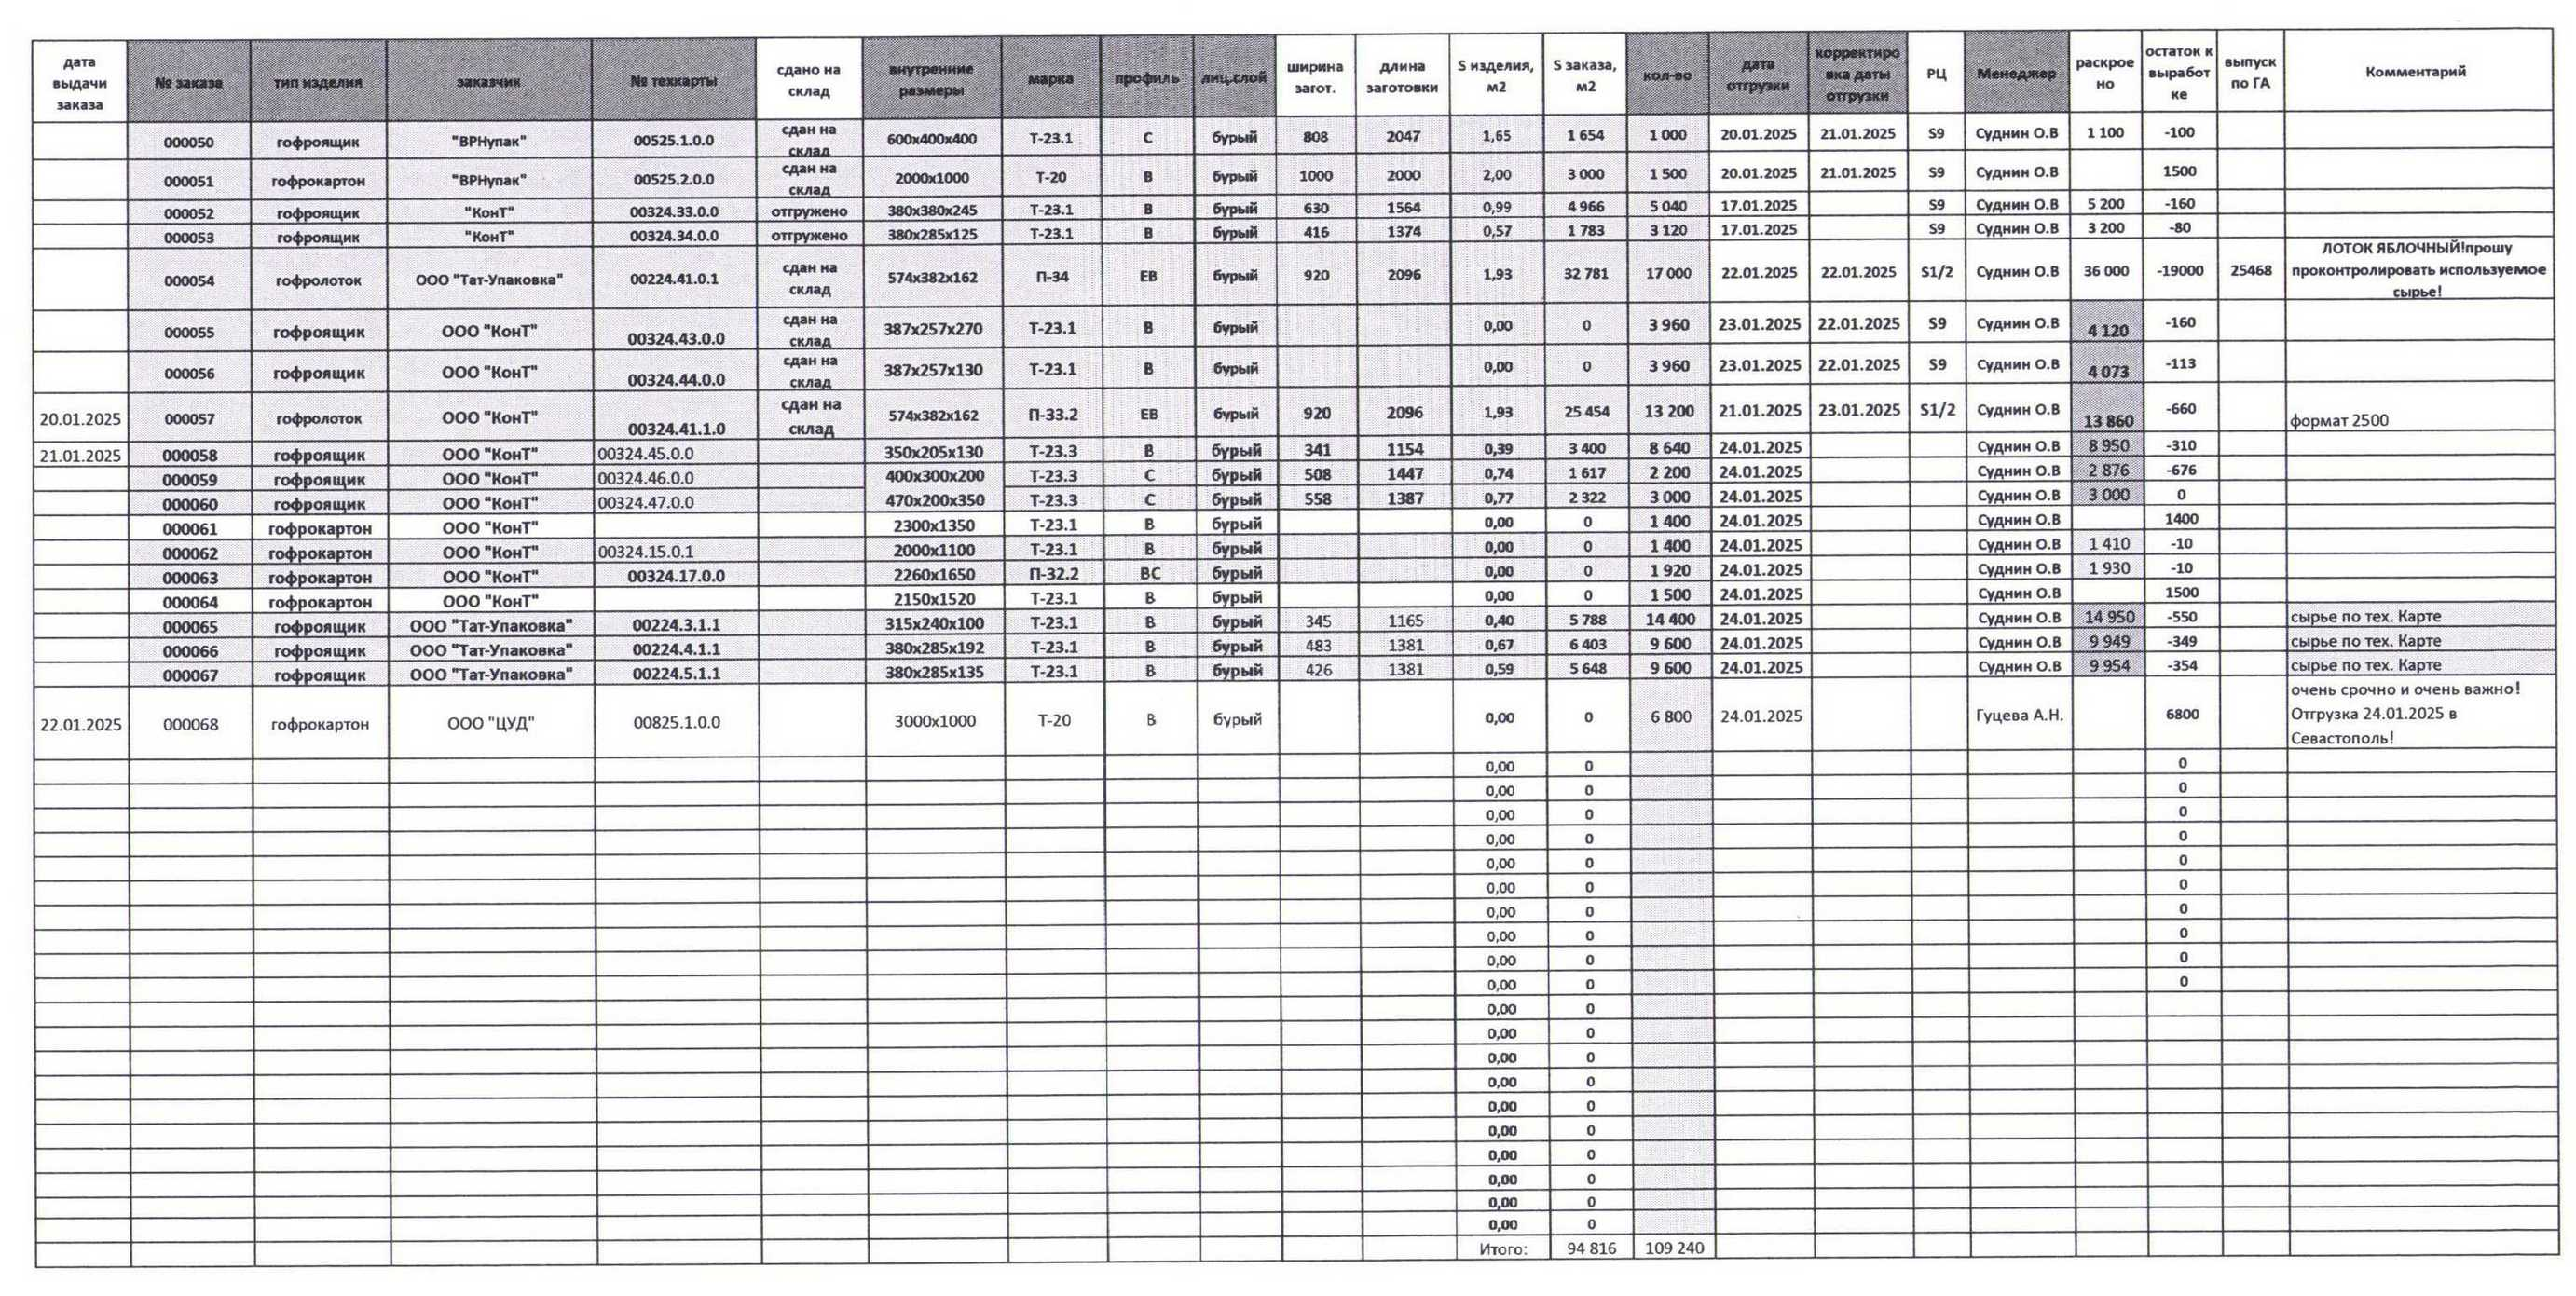
\includegraphics[width=\linewidth, height=0.94\textheight, angle=90, keepaspectratio]{Pics/f18.jpg}
\end{center}
\caption{Задание на смену для колориста}
\label{pic:f18}
\end{figure}

\begin{figure}
\begin{center}
 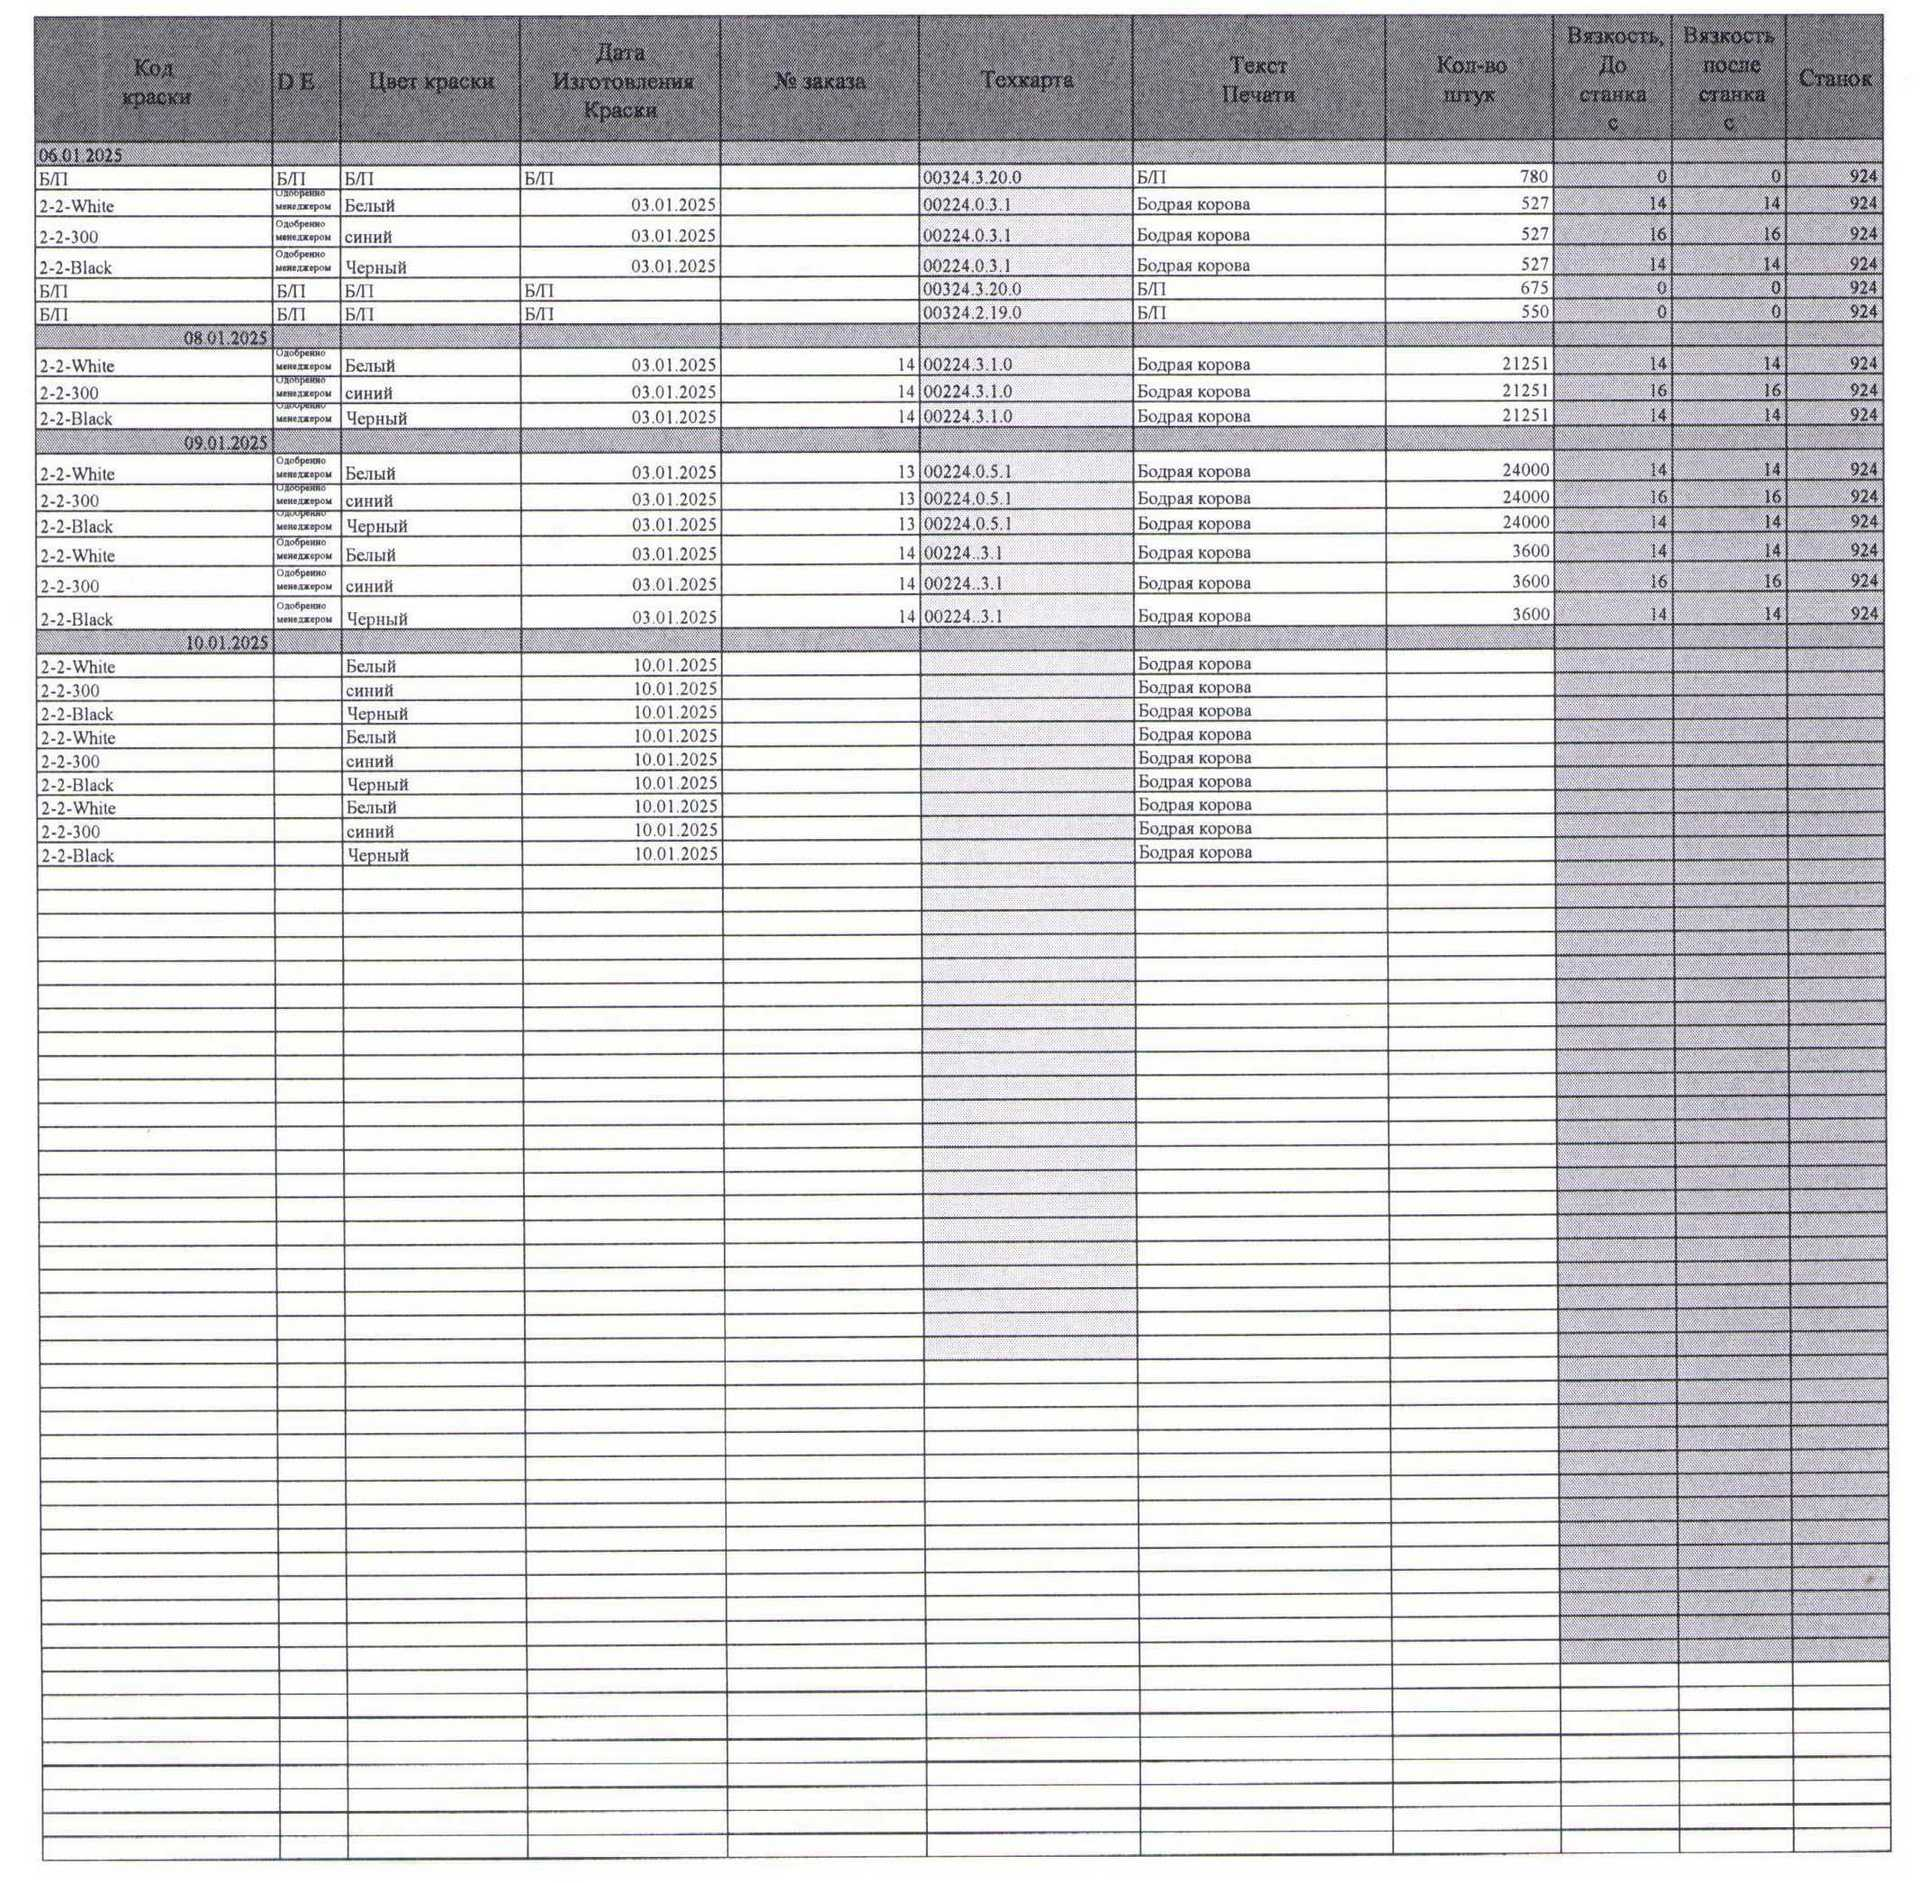
\includegraphics[width=\linewidth, height=0.94\textheight, angle=90, keepaspectratio]{Pics/f19.jpg}
\end{center}
\caption{Учет выдачи готовой краски на производство. Часть 1}
\label{pic:f19}
\end{figure}

\begin{figure}
\begin{center}
 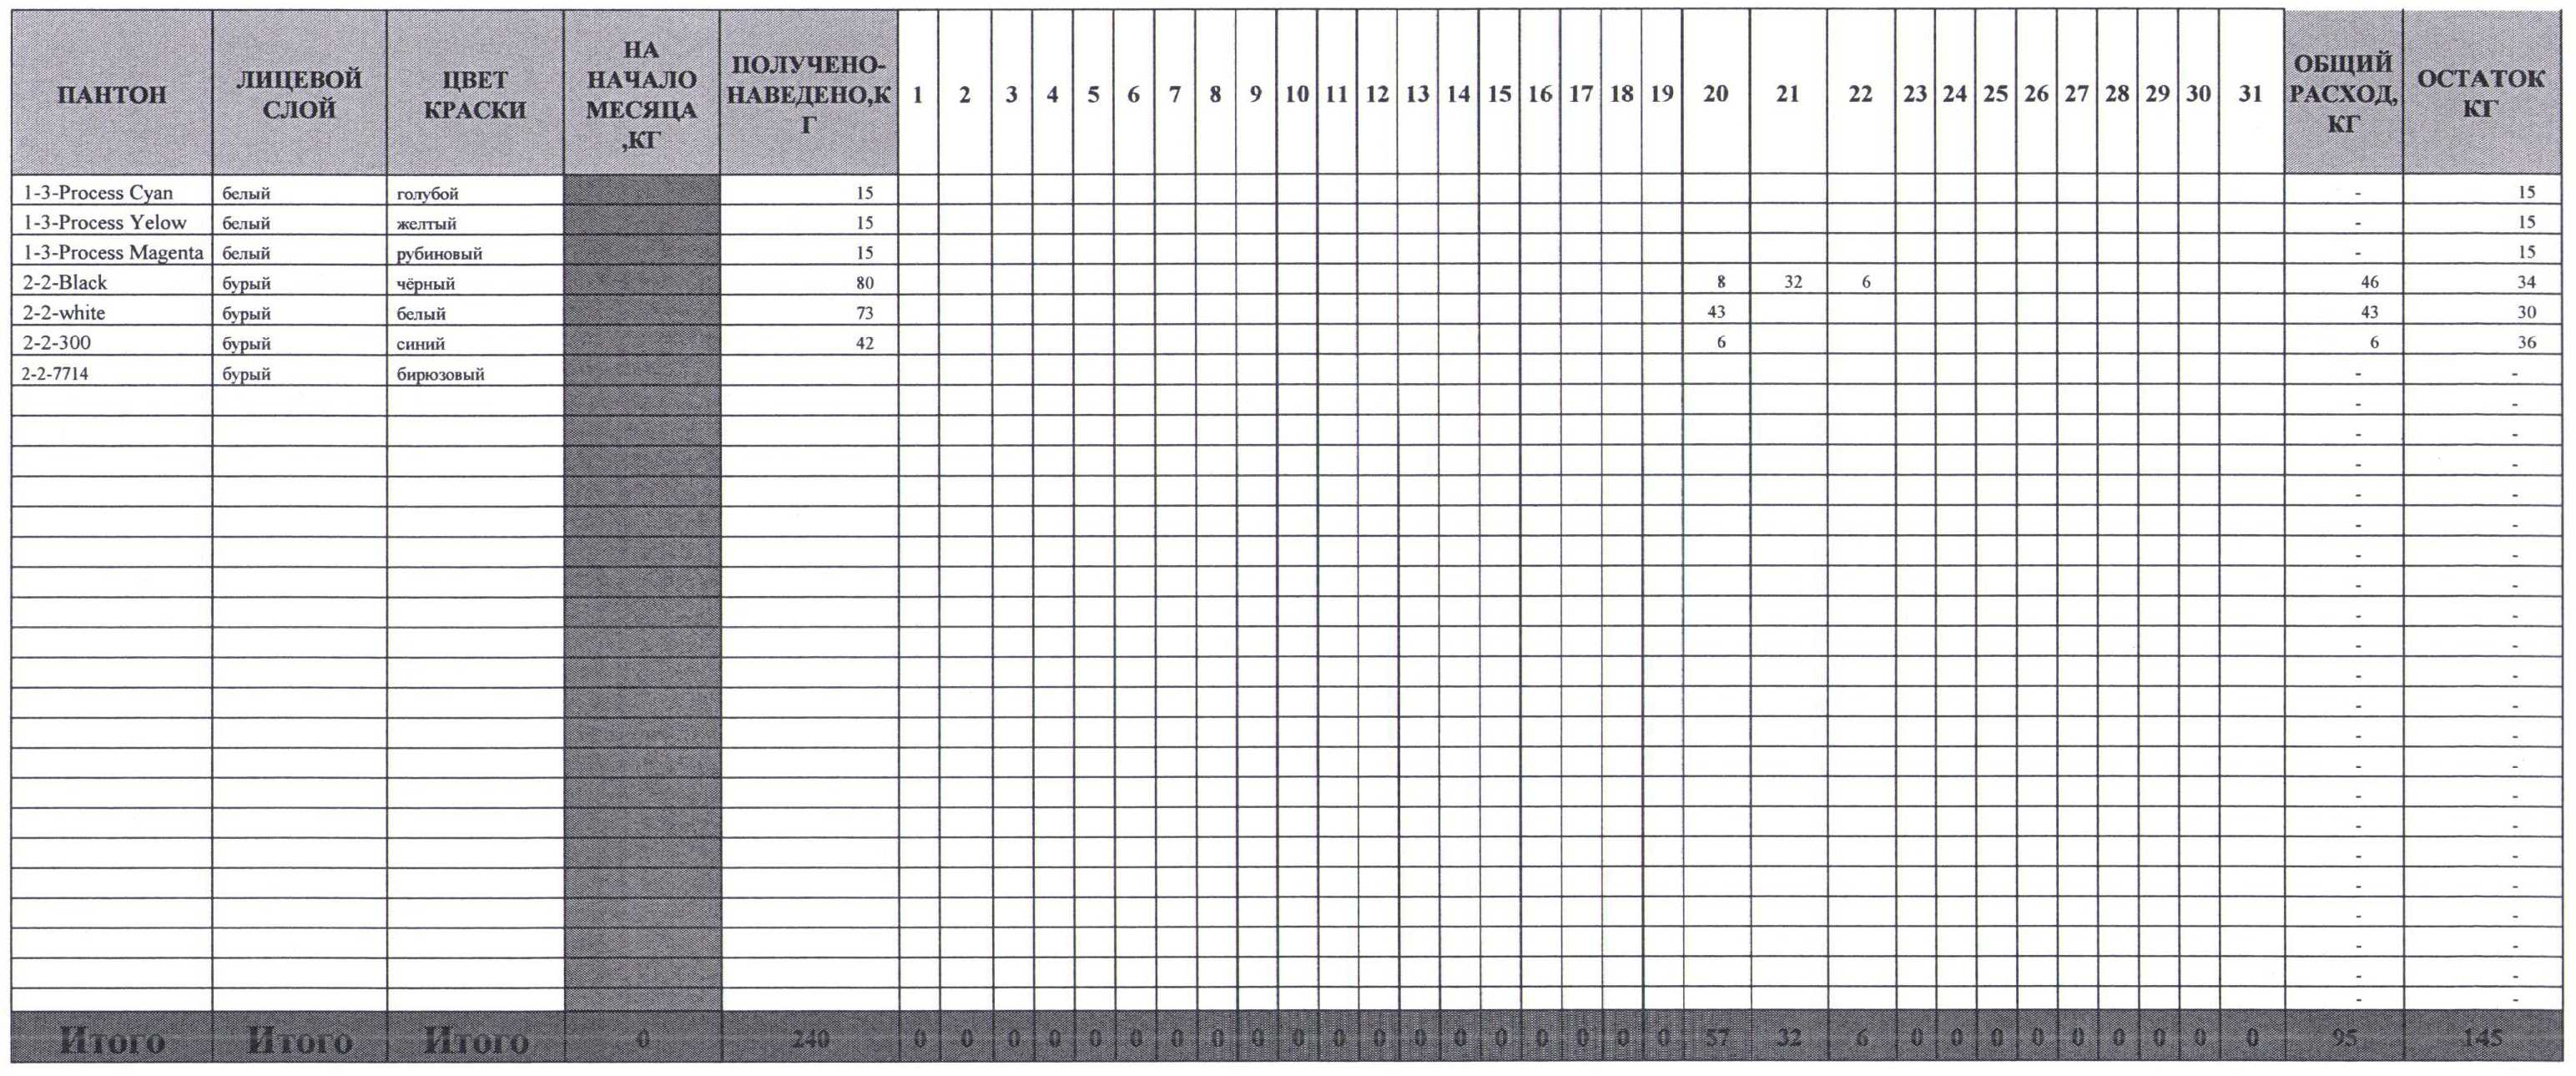
\includegraphics[width=\linewidth, height=0.94\textheight, angle=90, keepaspectratio]{Pics/f20.jpg}
\end{center}
\caption{Учет выдачи готовой краски на производство. Часть 2}
\label{pic:f20}
\end{figure}

\begin{figure}
\begin{center}
 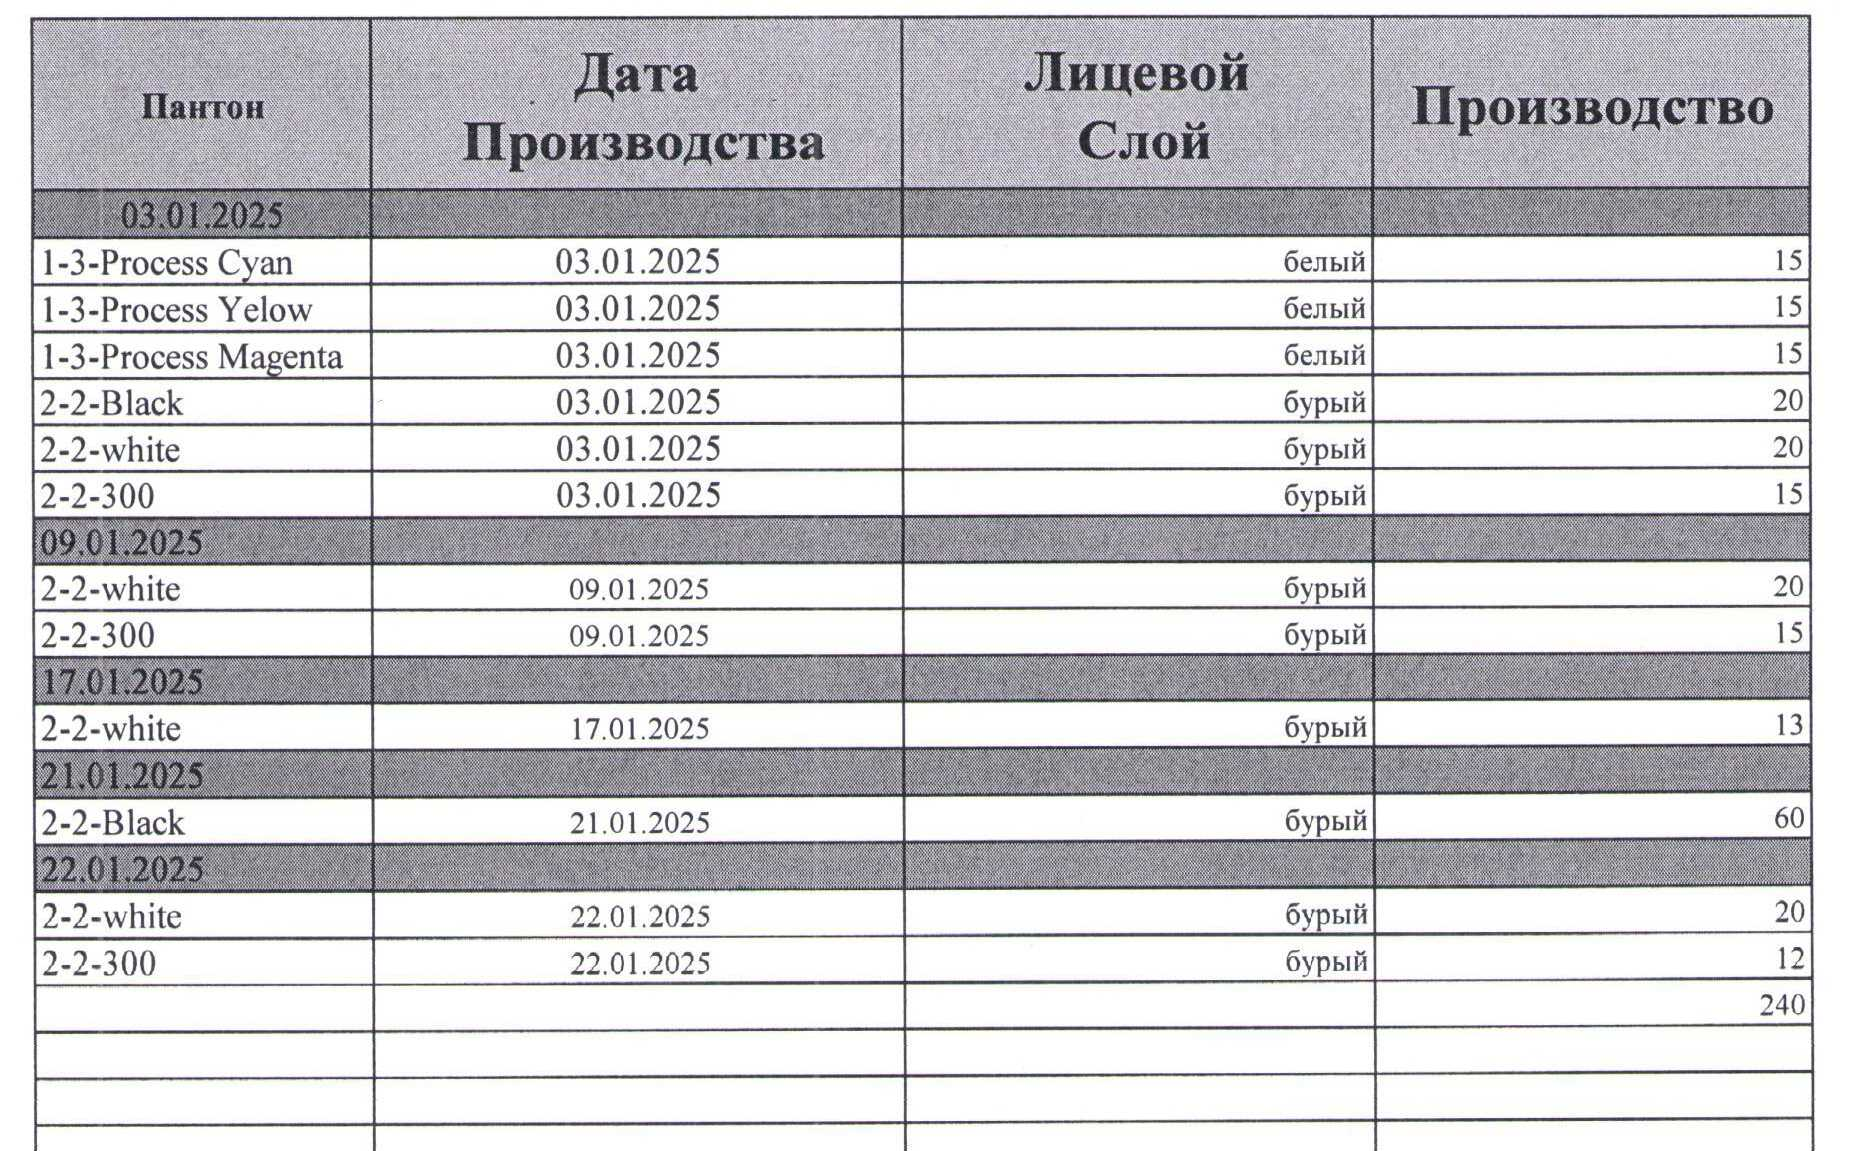
\includegraphics[width=\linewidth, height=0.94\textheight, keepaspectratio]{Pics/f21.jpg}
\end{center}
\caption{Баланс по краске}
\label{pic:f21}
\end{figure}




\clearpage
\ifx \notincludehead\undefined
\normalsize
\end{document}
\fi

\clearpage
% \ifx \notincludehead\undefined
\normalsize
\end{document}
\fi


\newpage
\subsection{Управление и диспетчеризация производства}
\label{bp:production}

% На производстве работает 16 машинистов, 2 погрузчика (водителя), 1 грузчик, 1 инженер технолог, 1 инженер качества, 1 комплектовщик оснастки, 1 мастер смены.


Производство работает в одну смену. 





\textbf{Выработка гофроагрегата}


Мастер смены выдает задание на ГА (рис. \ref{pic:f29}). Машинист вбивает данные на продольной и поперечной резках в систему управления заказами на гофроагрегате Hsieh Hsu.

Бригадир передает в устной форме на склад запрос на поставку необходимого сырья, предварительно посмотрев <<домоты>> (остатки по рулонам). Бригадир совместно с кладовщиком заполняют ведомость по сырью (рис. \ref{pic:f26}). Переданный на производство со склада рулон сразу списывается с учета.


Машинисты запускают ГА, производят гофрокартон согласно  планового задания. 

Данные по выработке вносят в MS EXCEL (рис. \ref{pic:f23}).

Бирки на полуфабрикаты, выпущенные на ГА, машинисты печатают (рис. \ref{pic:f31}) сразу на весь заказ. Бирки печатаются непосредственно на ГА. Механизм автоматического формирования бирок не настроен.

По факту выработки с гофроагрегата машинист формирует отчет по выработке по форме (рис. \ref{pic:d6}).




\textbf{Выработка линии переработки}

Мастер смены выдает машинистам задания по линиям (рис. \ref{pic:f24}). Технологические карты бригадиры печатают с сервера. 
Краску, при возникновении необходимости, выдает колорист.
Оснастку машинисты берут сами. Оснастка хранится около производственных линий.
Машинисты настраивают машину и выпускают продукцию согласно требованиям ТК.


Бирки на готовую продукцию печатает мастер сразу на весь заказ и с плановым заданием передает на линию (рис. \ref{pic:f30}).

Выработку машинисты на линиях вносят в файл MS EXCEL  (рис. \ref{pic:f23}).


Бригадиры на перерабатывающих линиях ведут таблицу MS EXCEL с указанием простоев (рис. \ref{pic:f28}. Подробнее процесс описан в разделе \ref{bp:maintance}).

В конце смены на основании данных по выработкам из таблицы MS EXCEL мастер заполняет отчет производства за смену (рис. \ref{pic:f25}).

Также мастер заполняет ведомость передачи ГП на склад и сверяется с данными кладовщика готовой продукции (рис. \ref{pic:f6}).




\begin{figure}
\begin{center}
 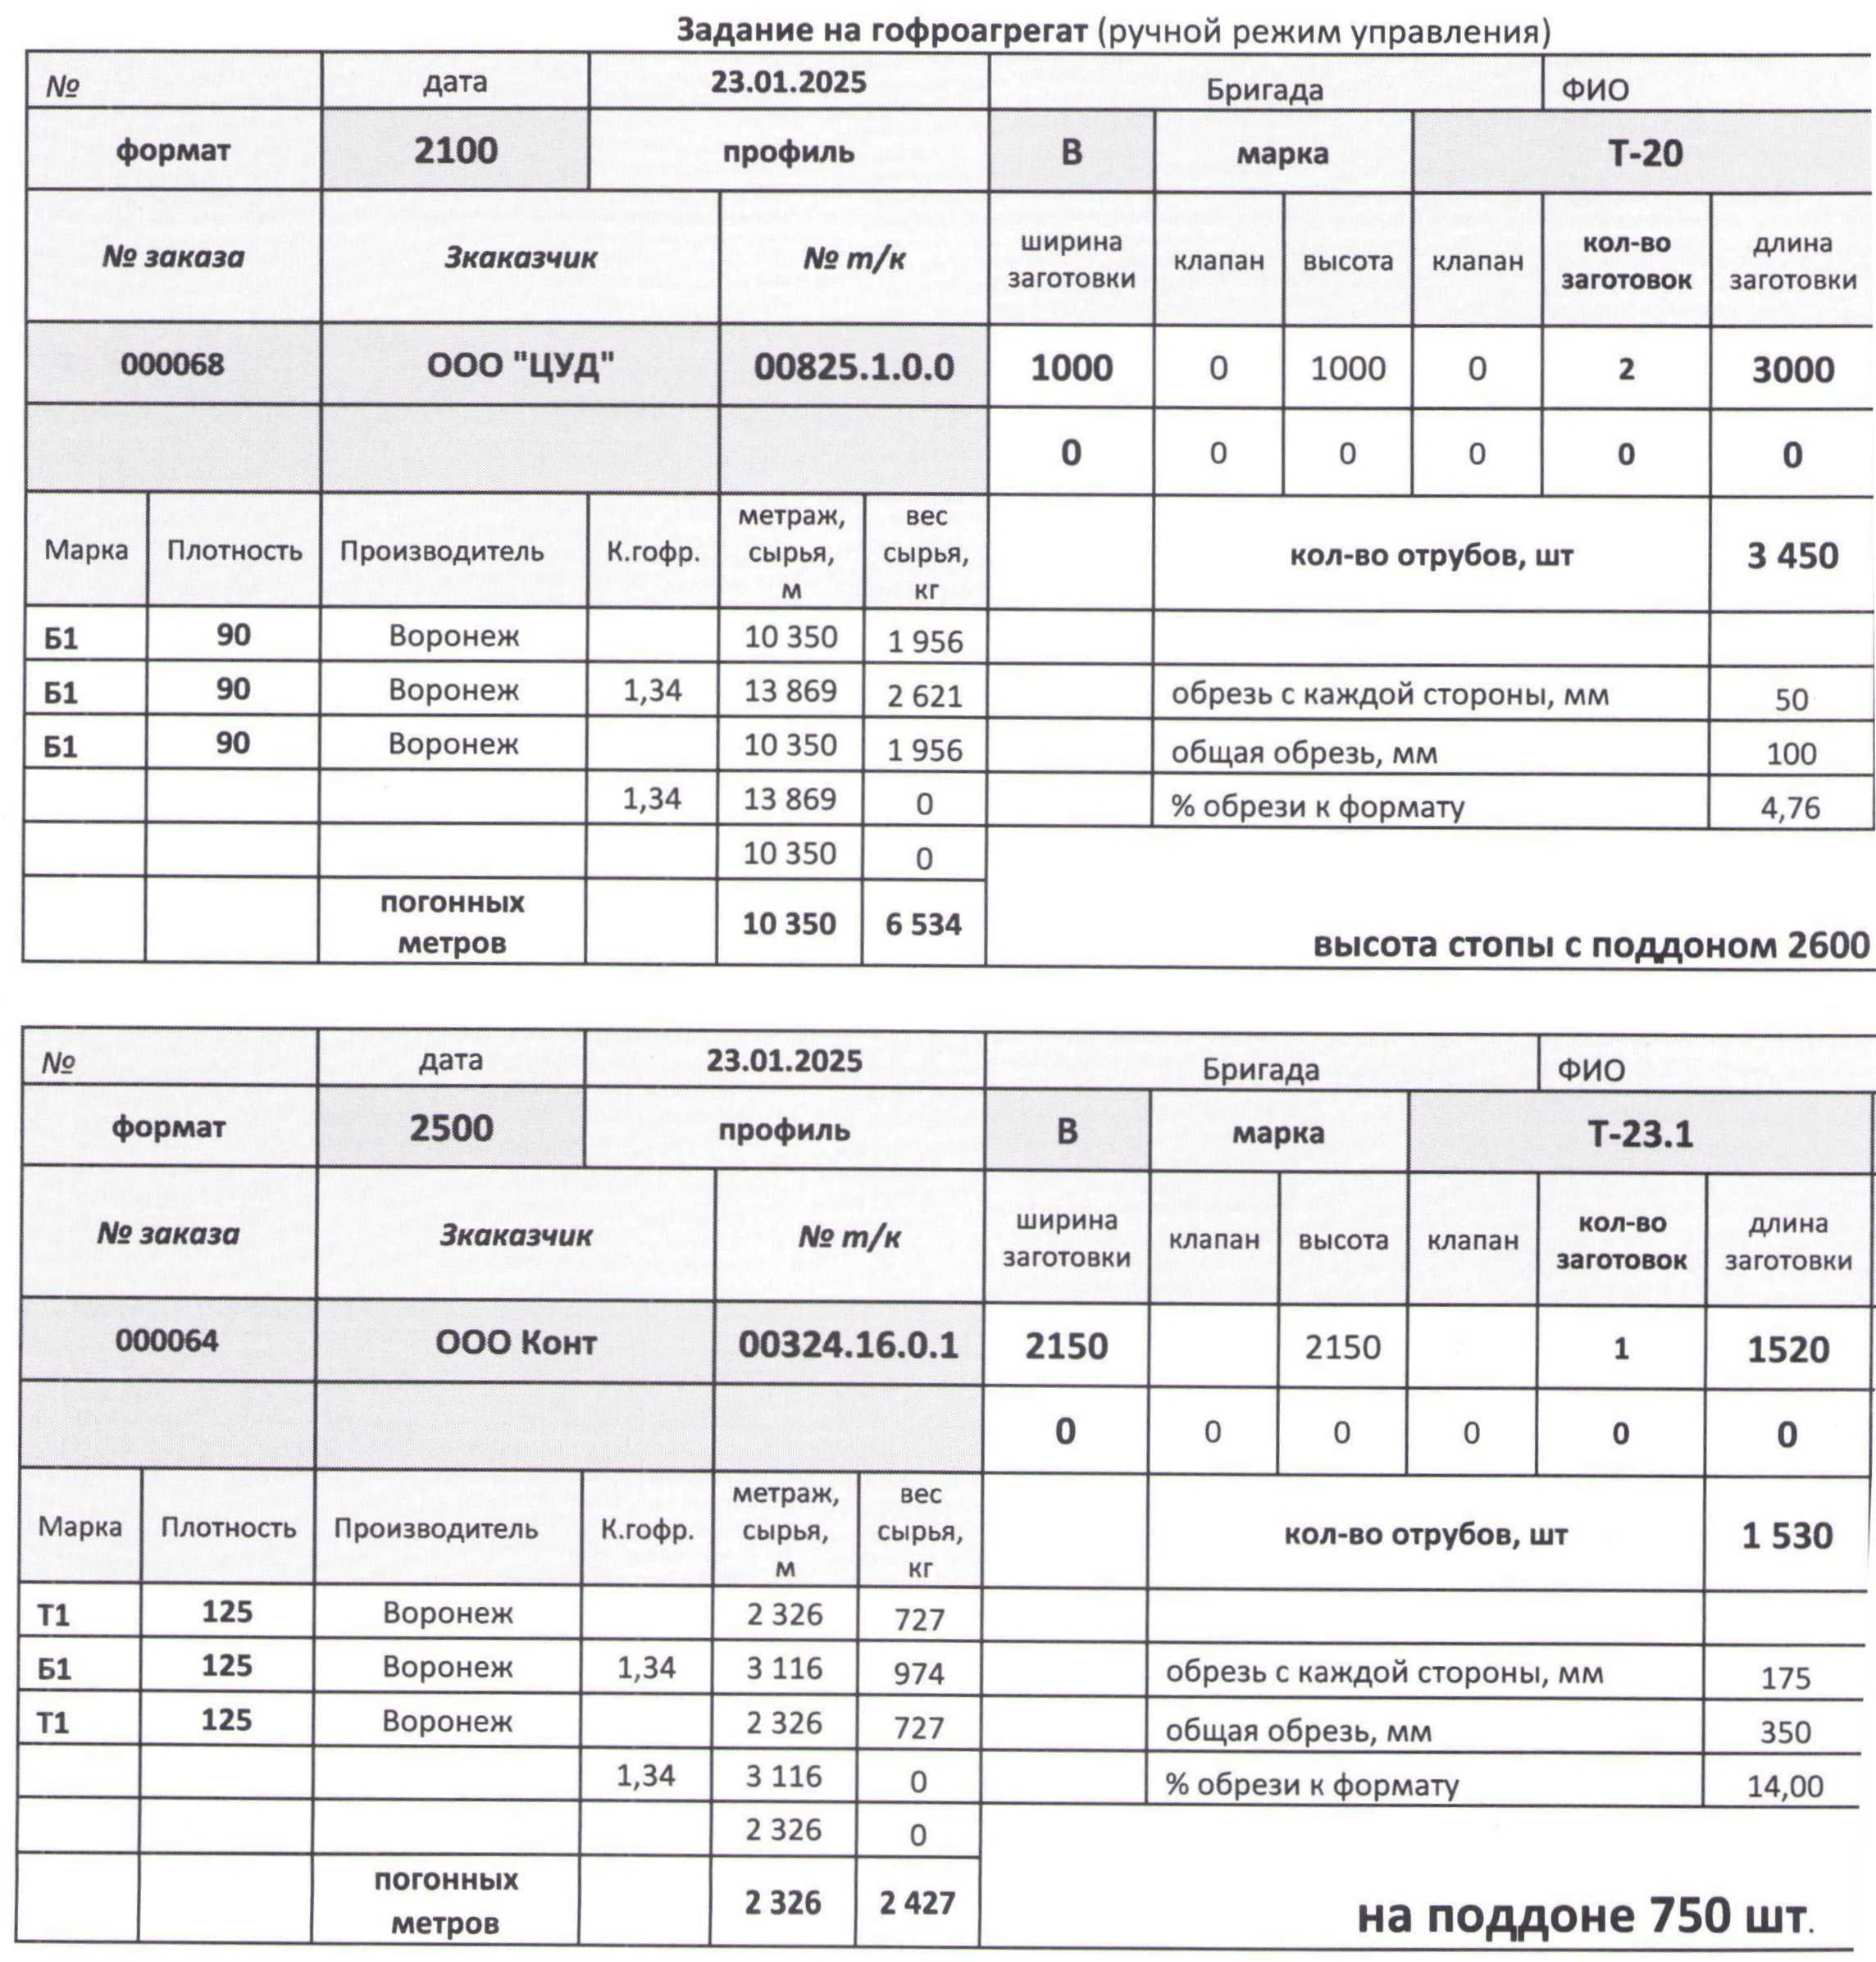
\includegraphics[width=\linewidth, height=0.94\textheight, keepaspectratio]{Pics/f29.jpg}
\end{center}
\caption{Задание на смену для ГА}
\label{pic:f29}
\end{figure}

\begin{figure}
\begin{center}
 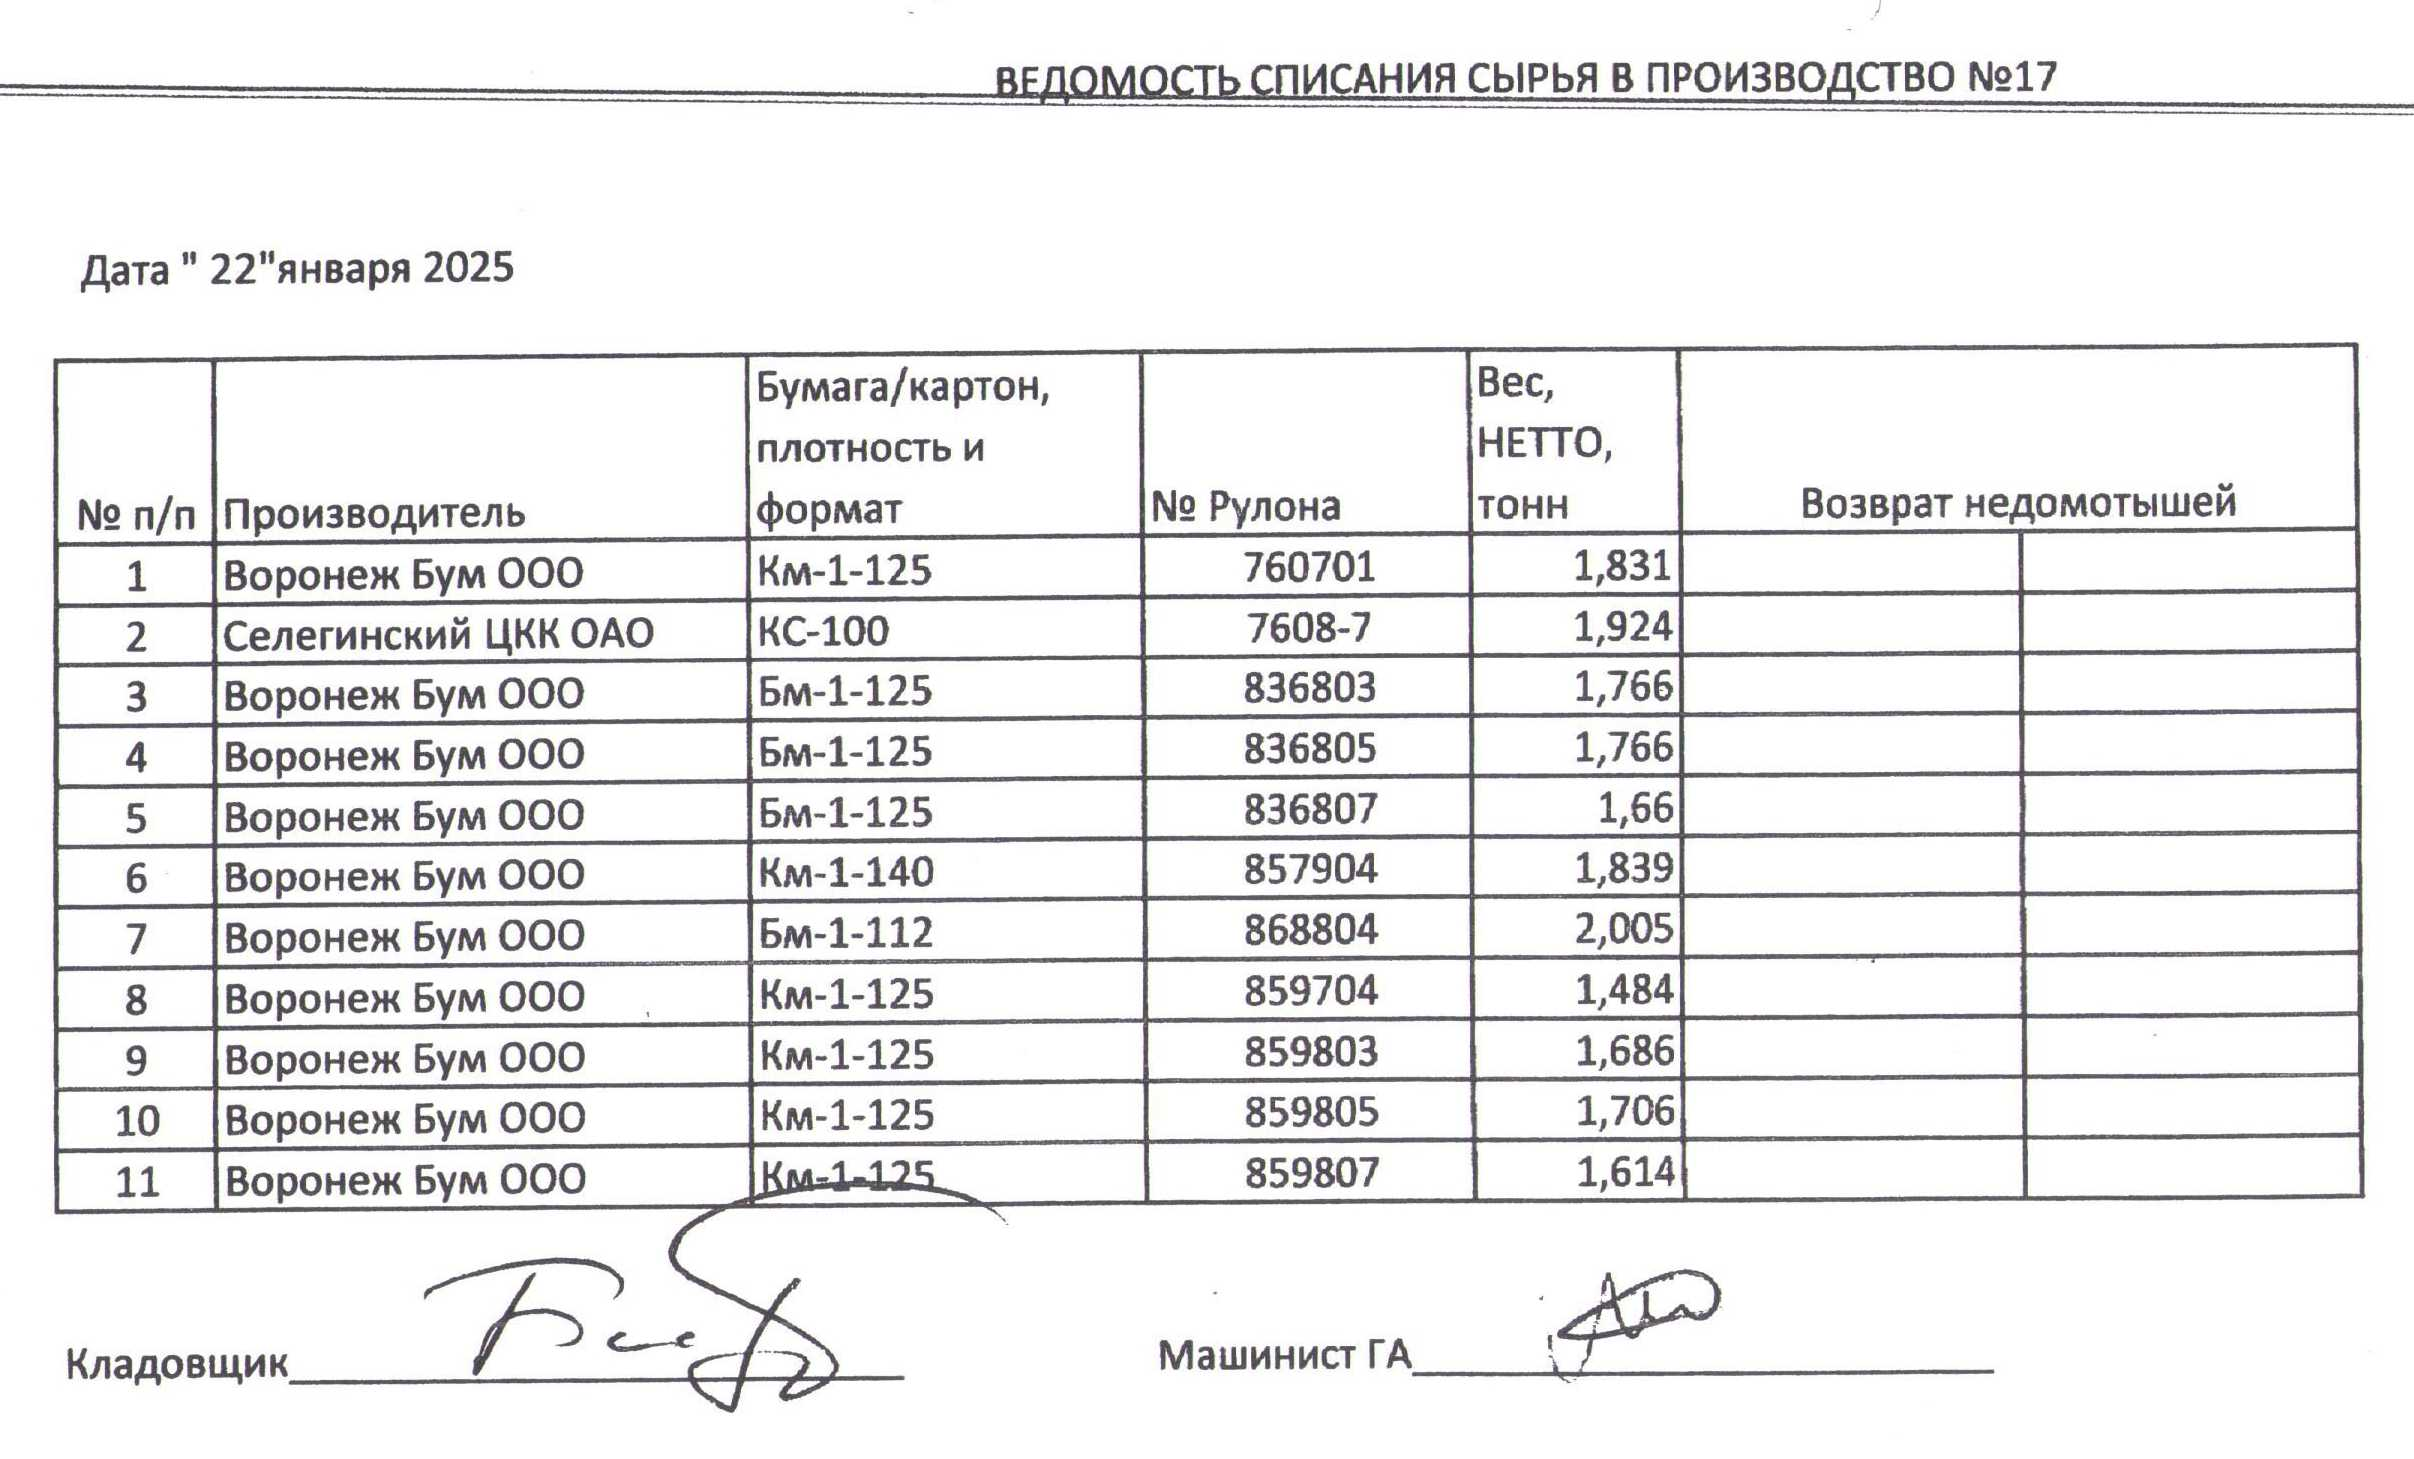
\includegraphics[width=\linewidth, height=0.94\textheight, keepaspectratio]{Pics/f26.jpg}
\end{center}
\caption{Ведомость по сырью}
\label{pic:f26}
\end{figure}

\begin{figure}
\begin{center}
 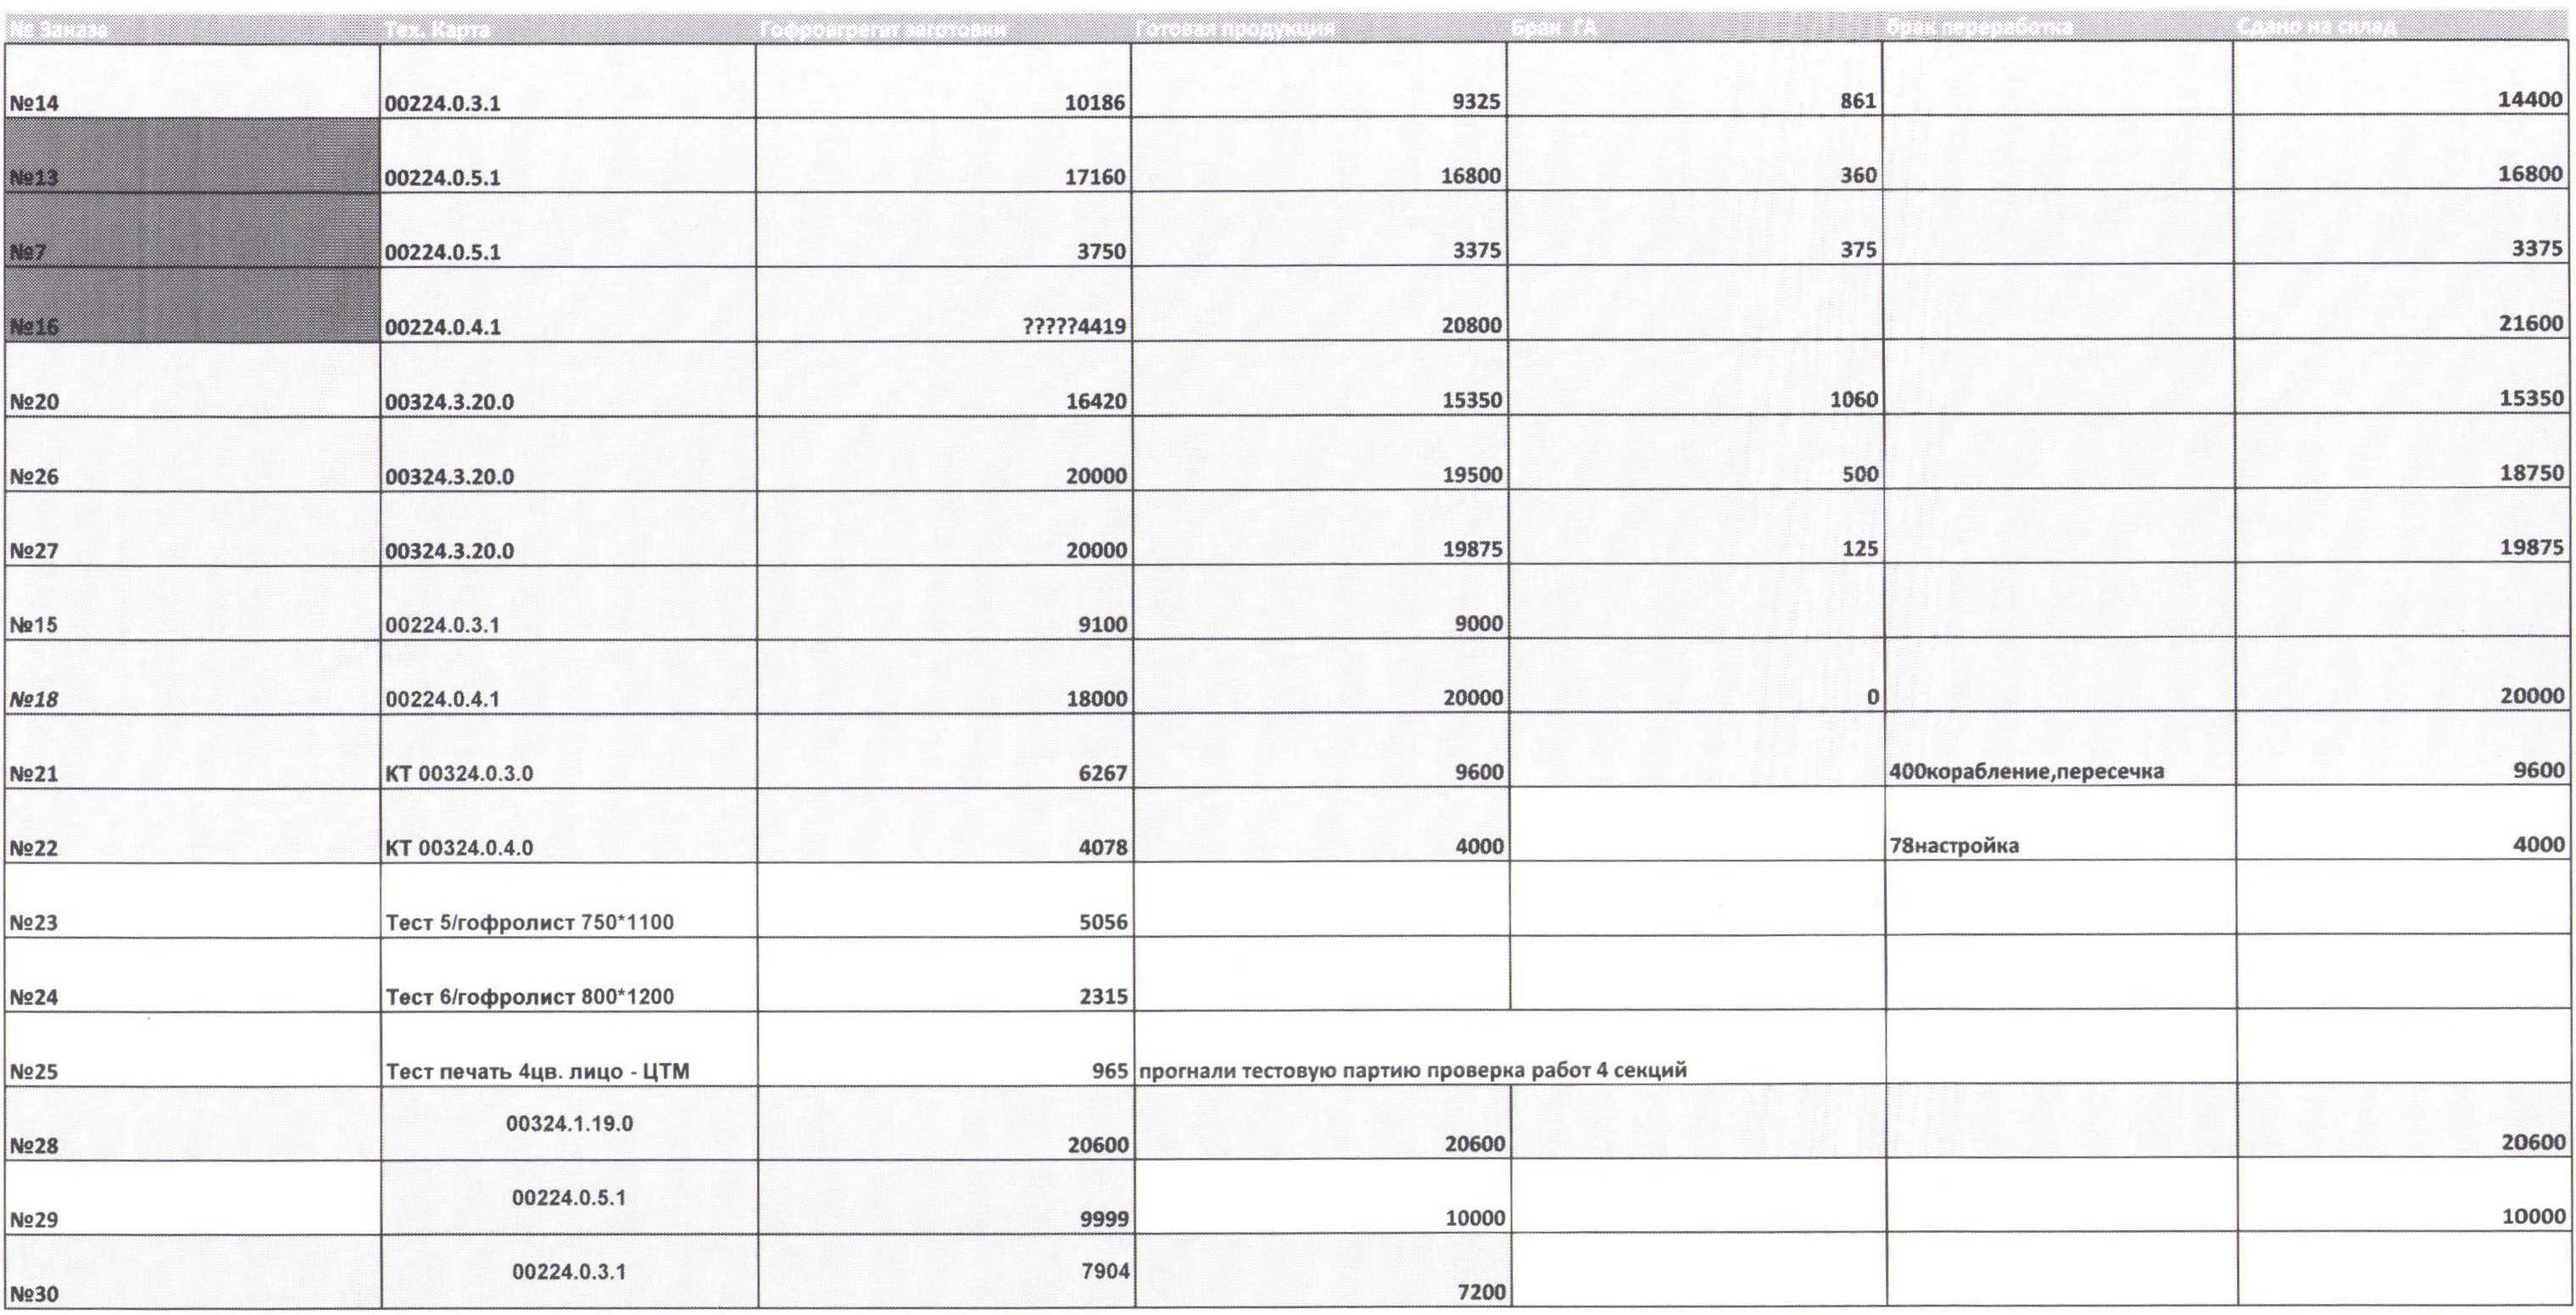
\includegraphics[width=\linewidth, height=0.94\textheight, keepaspectratio]{Pics/f23.jpg}
\end{center}
\caption{Учет выработки}
\label{pic:f23}
\end{figure}

\begin{figure}
\begin{center}
 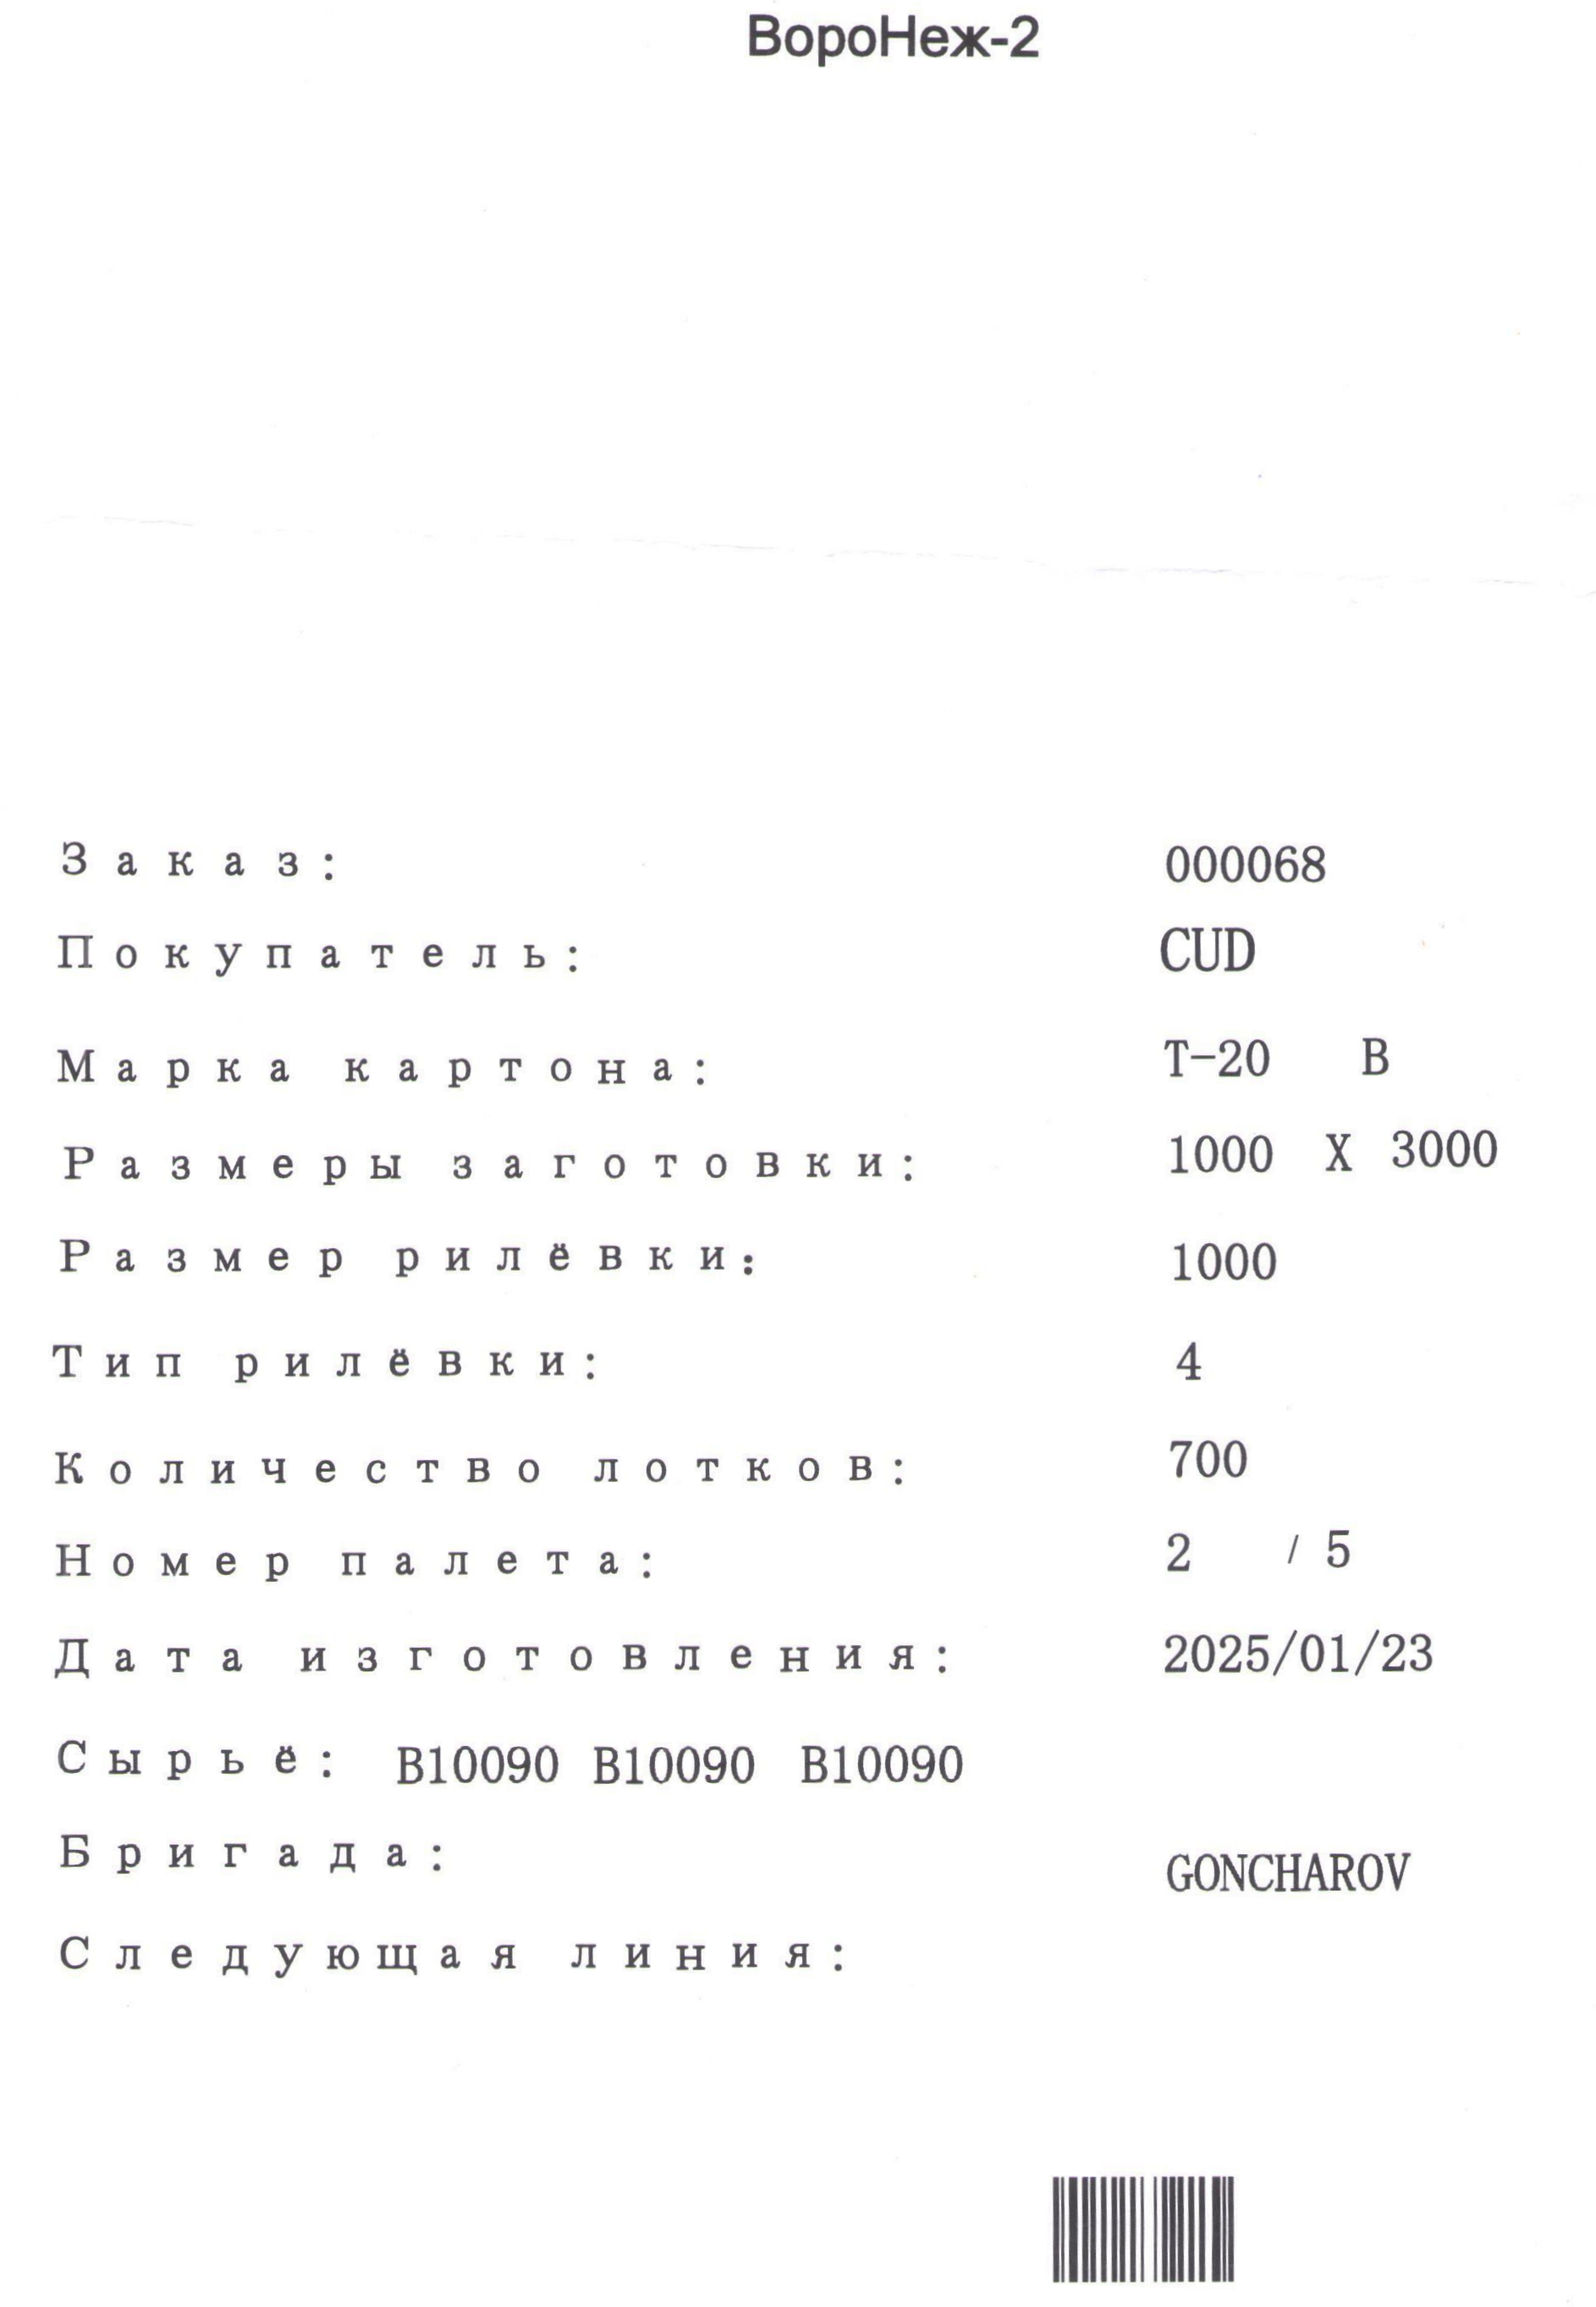
\includegraphics[width=\linewidth, height=0.94\textheight, keepaspectratio]{Pics/f31.jpg}
\end{center}
\caption{Бирки на ПФ}
\label{pic:f31}
\end{figure}

\begin{figure}
\begin{center}
 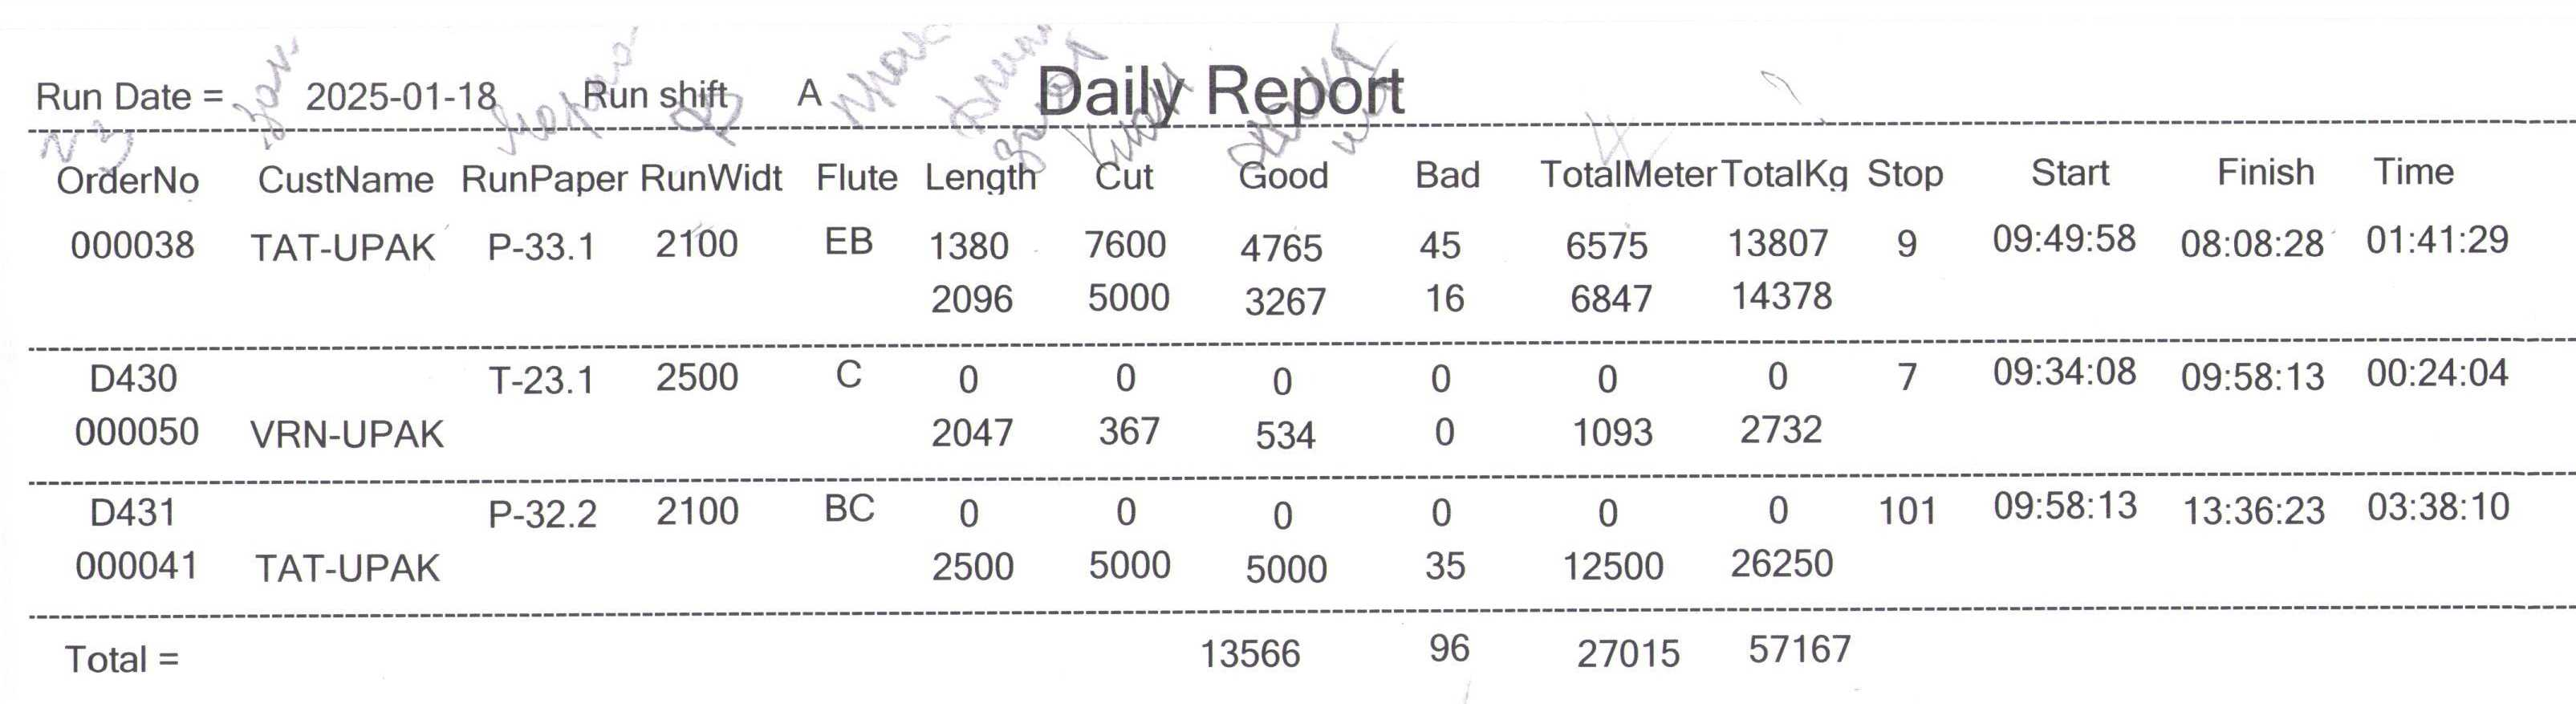
\includegraphics[width=\linewidth, height=0.94\textheight, keepaspectratio]{Pics/d6.jpg}
\end{center}
\caption{Отчет производства за смену ГА}
\label{pic:d6}
\end{figure}

\begin{figure}
\begin{center}
 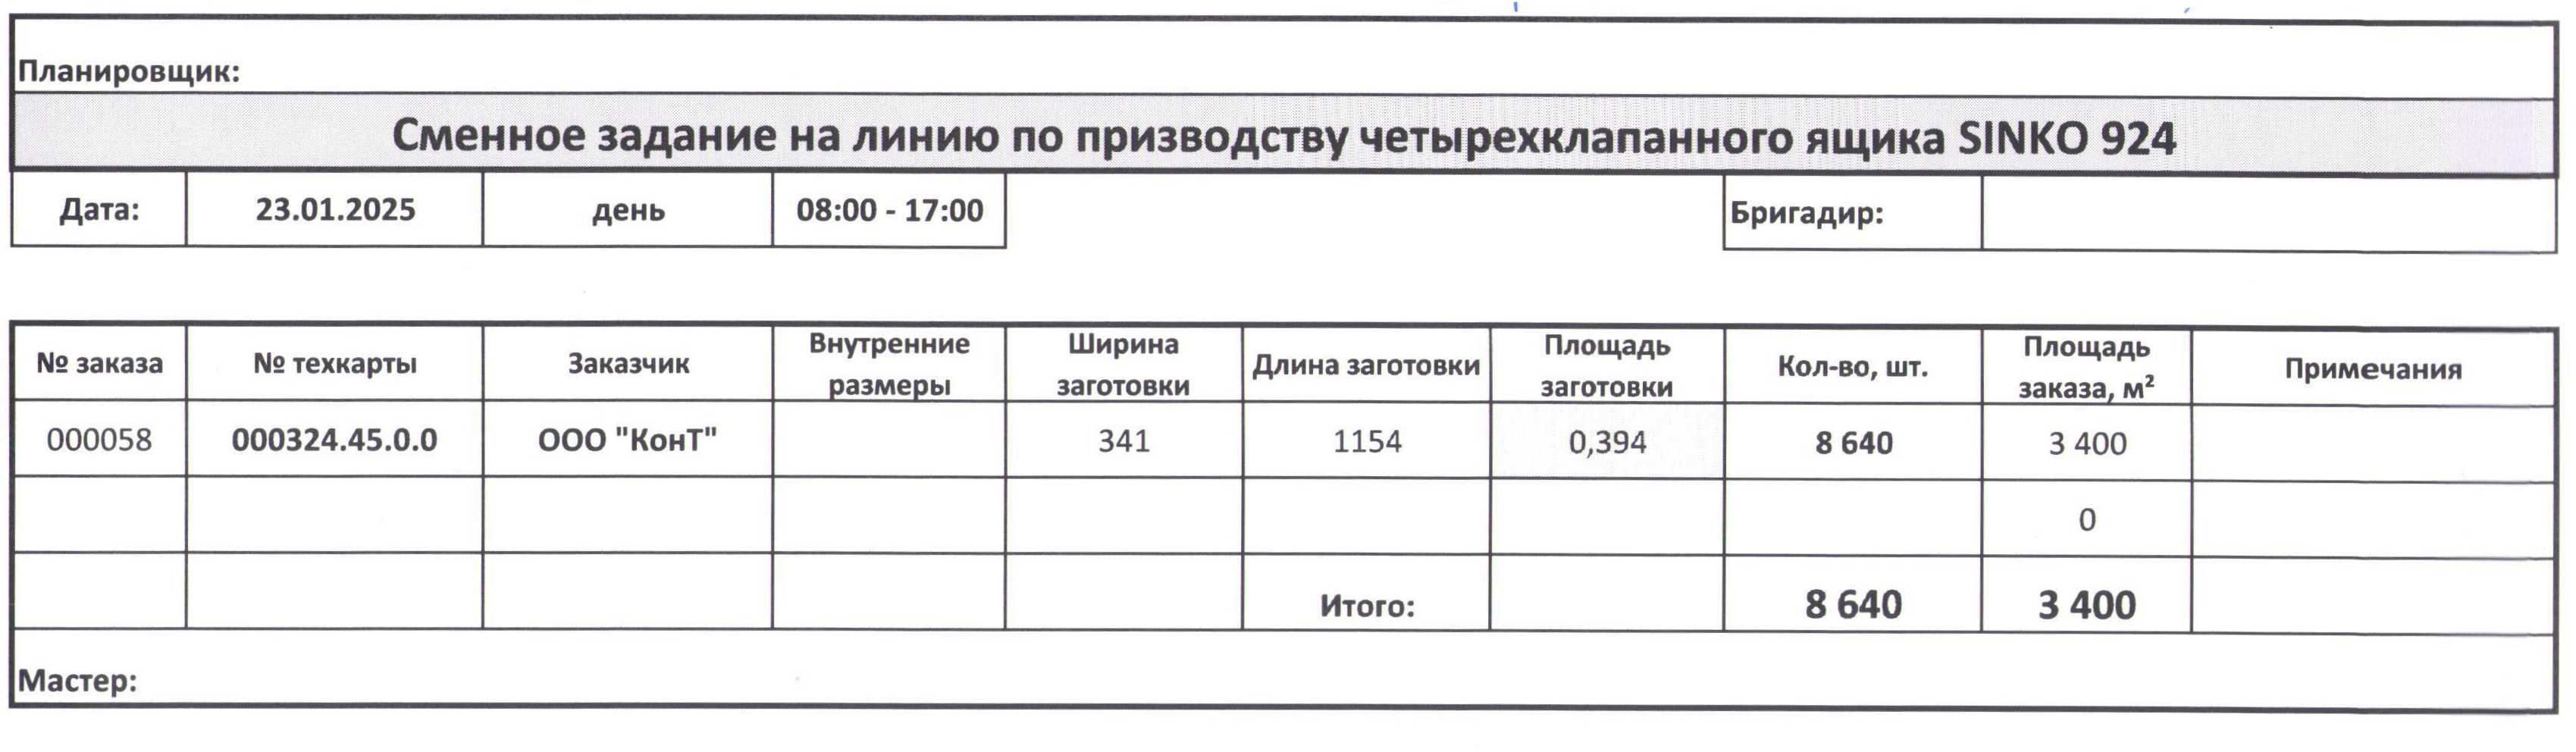
\includegraphics[width=\linewidth, height=0.94\textheight, keepaspectratio]{Pics/f24.jpg}
\end{center}
\caption{Задание на смену для ПЛ}
\label{pic:f24}
\end{figure}

\begin{figure}
\begin{center}
 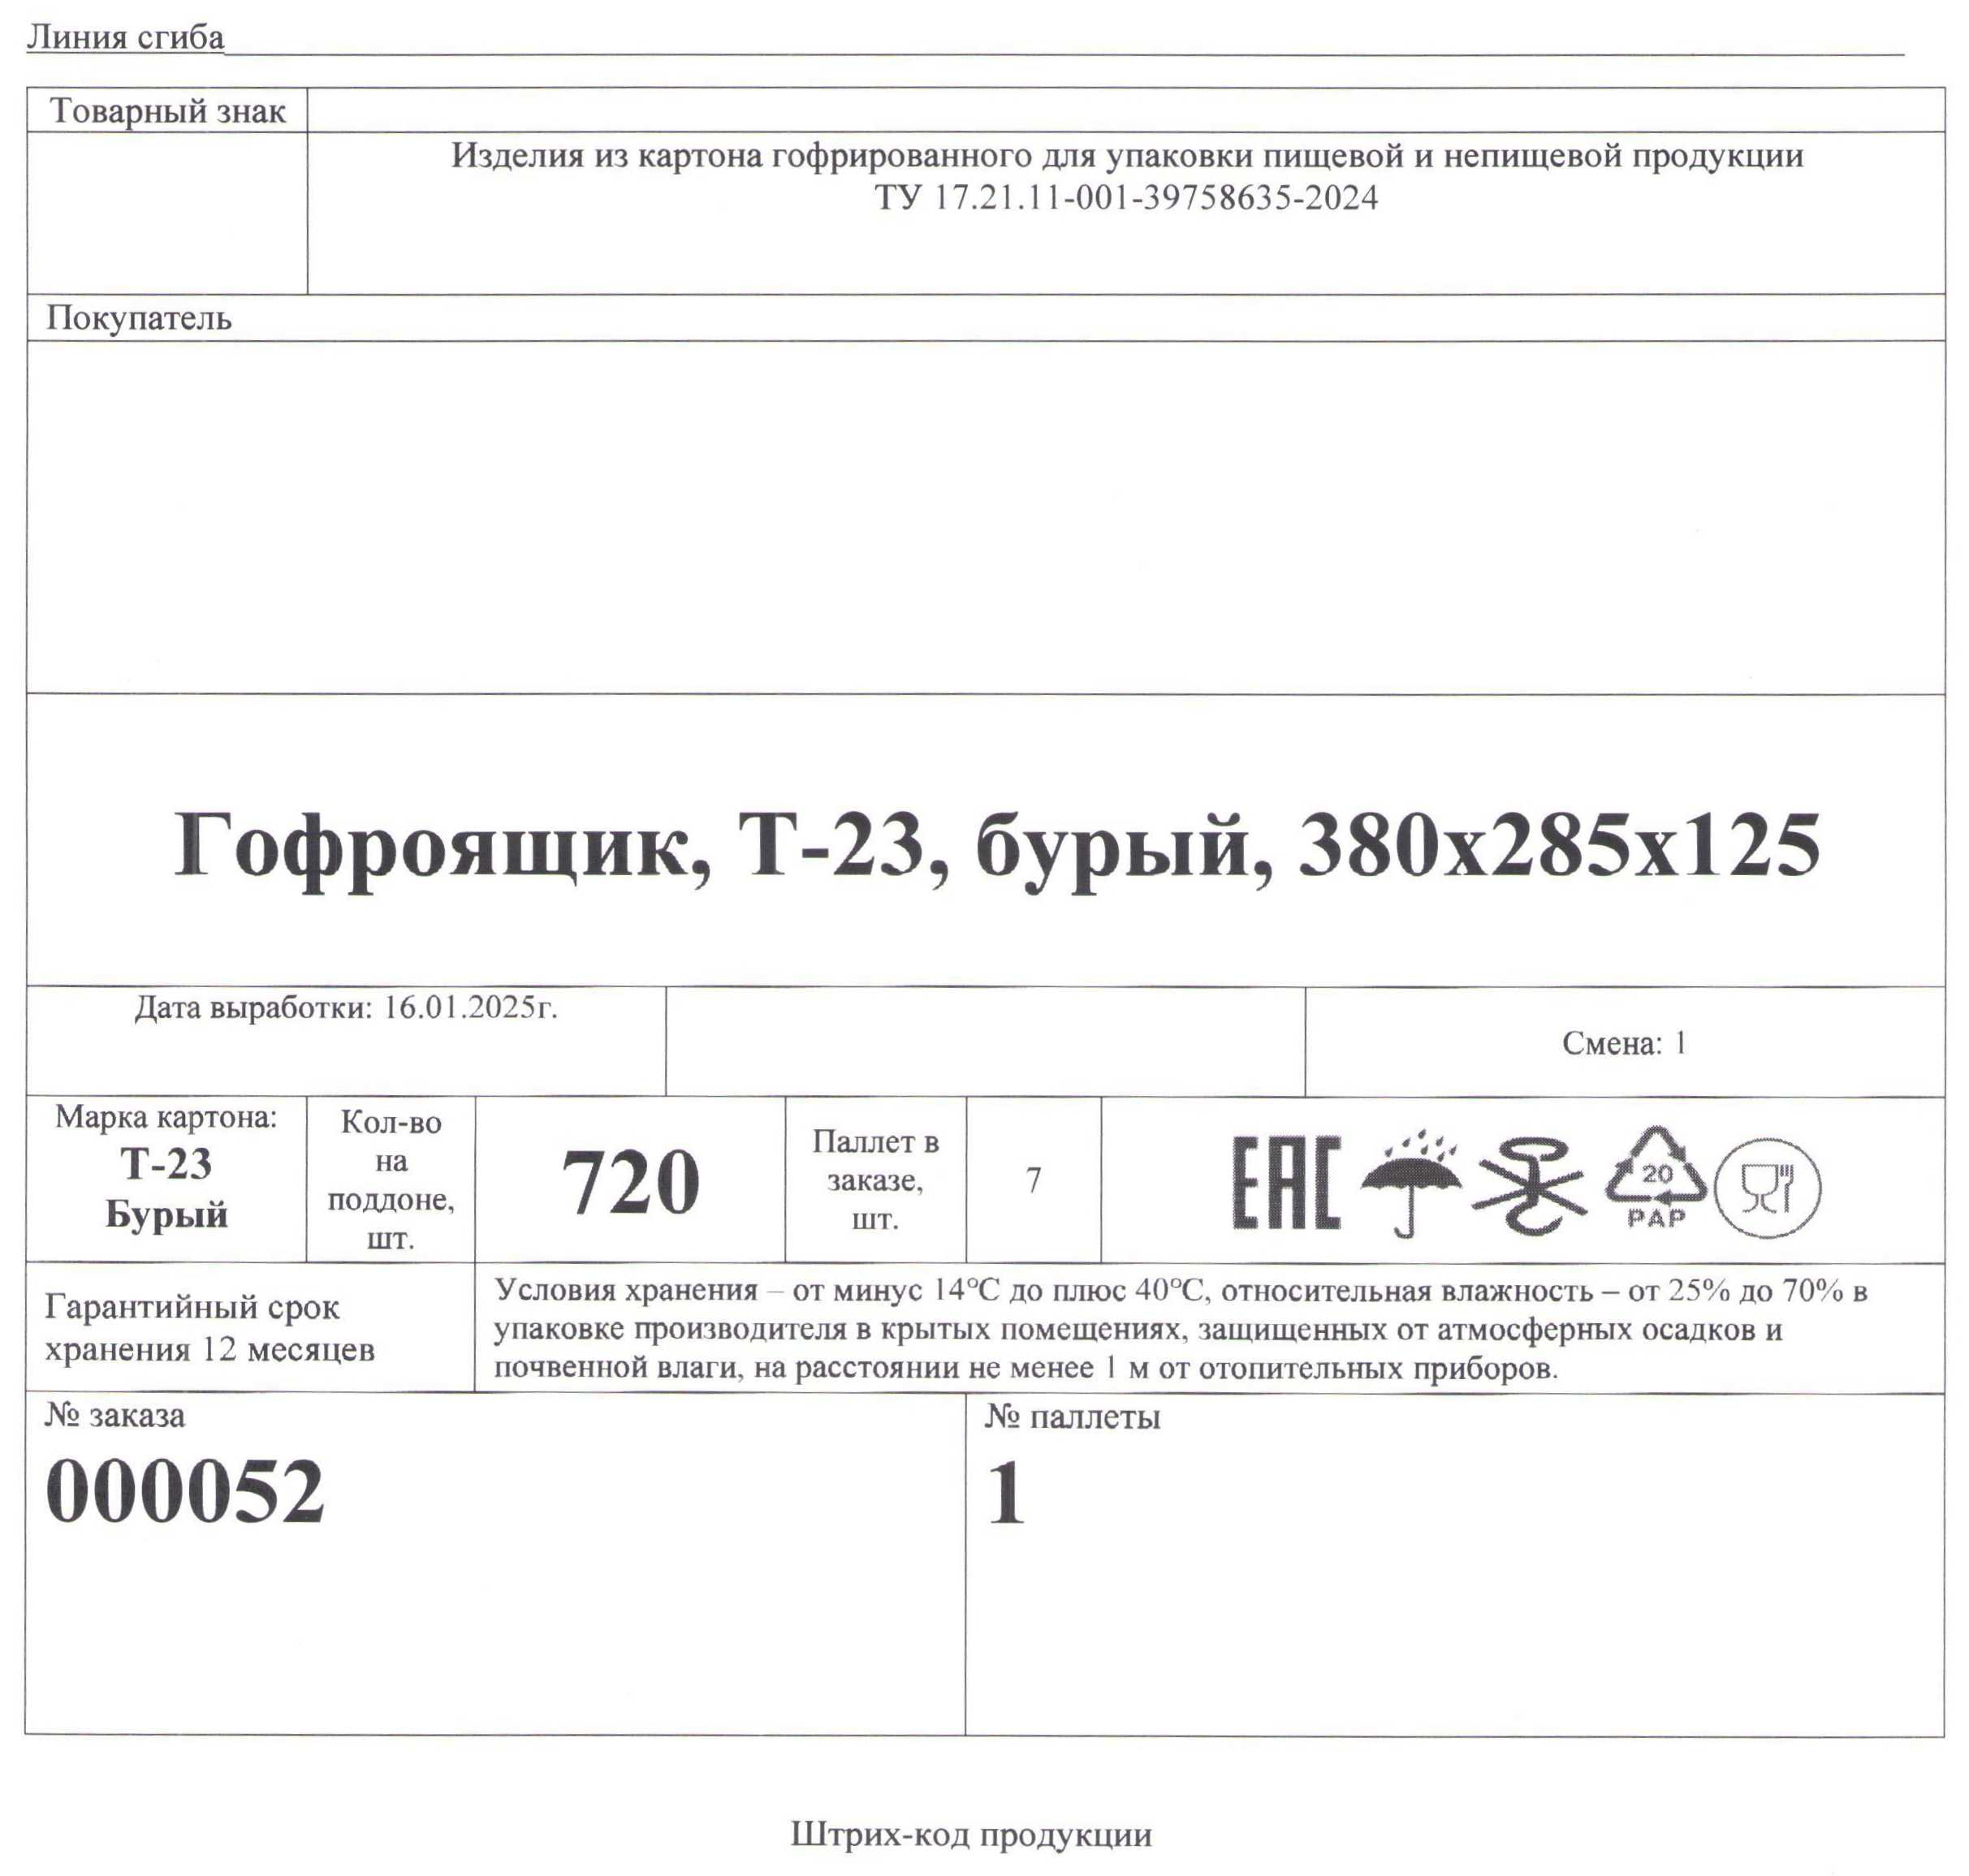
\includegraphics[width=\linewidth, height=0.94\textheight, keepaspectratio]{Pics/f30.jpg}
\end{center}
\caption{Бирки на ГП}
\label{pic:f30}
\end{figure}

\begin{figure}
\begin{center}
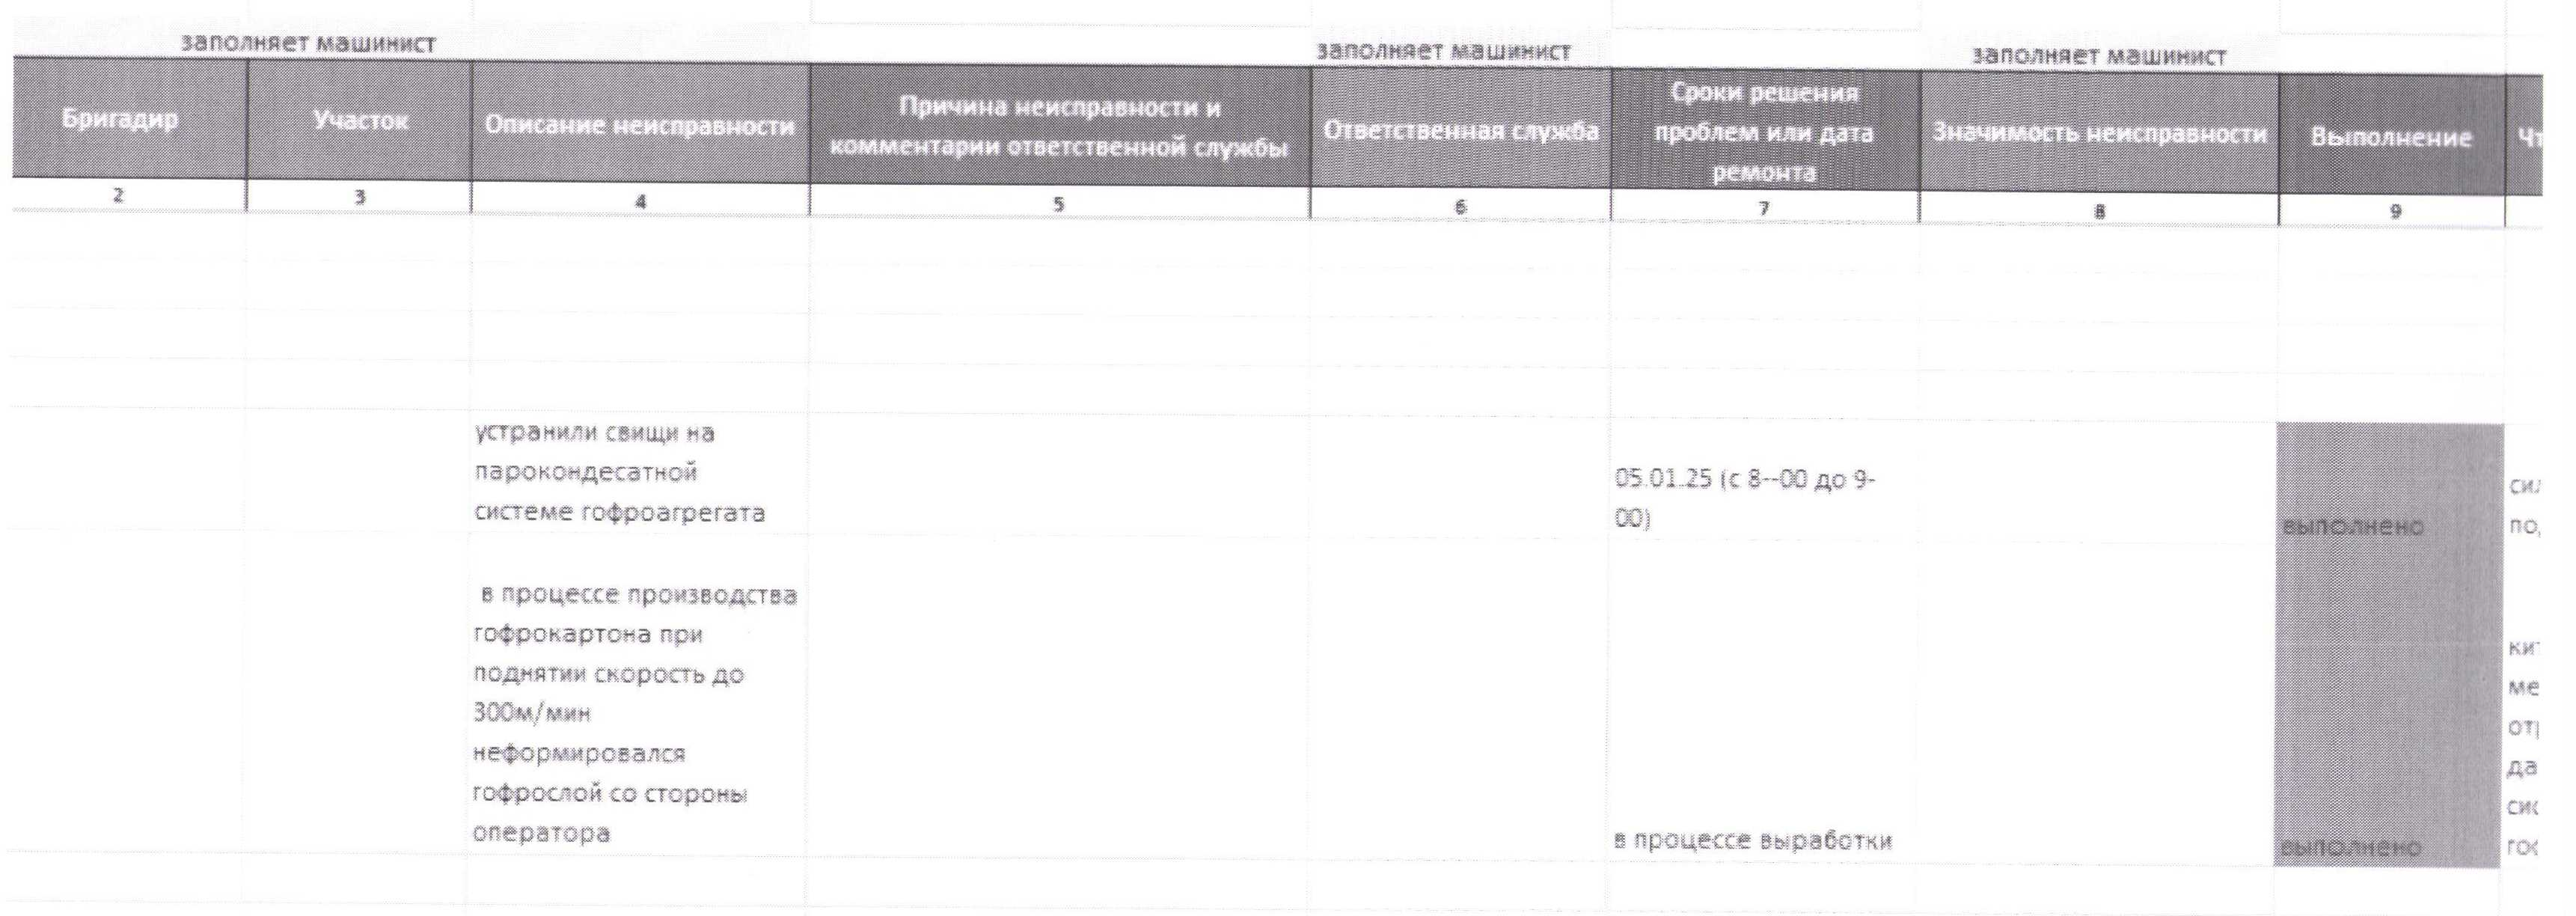
\includegraphics[height=0.94\textheight, width=\textwidth, angle=90, keepaspectratio]{Pics/f28.jpg}
\end{center}
\caption{Журнал простоев и неисправностей}
\label{pic:f28}
\end{figure}

\begin{figure}
\begin{center}
 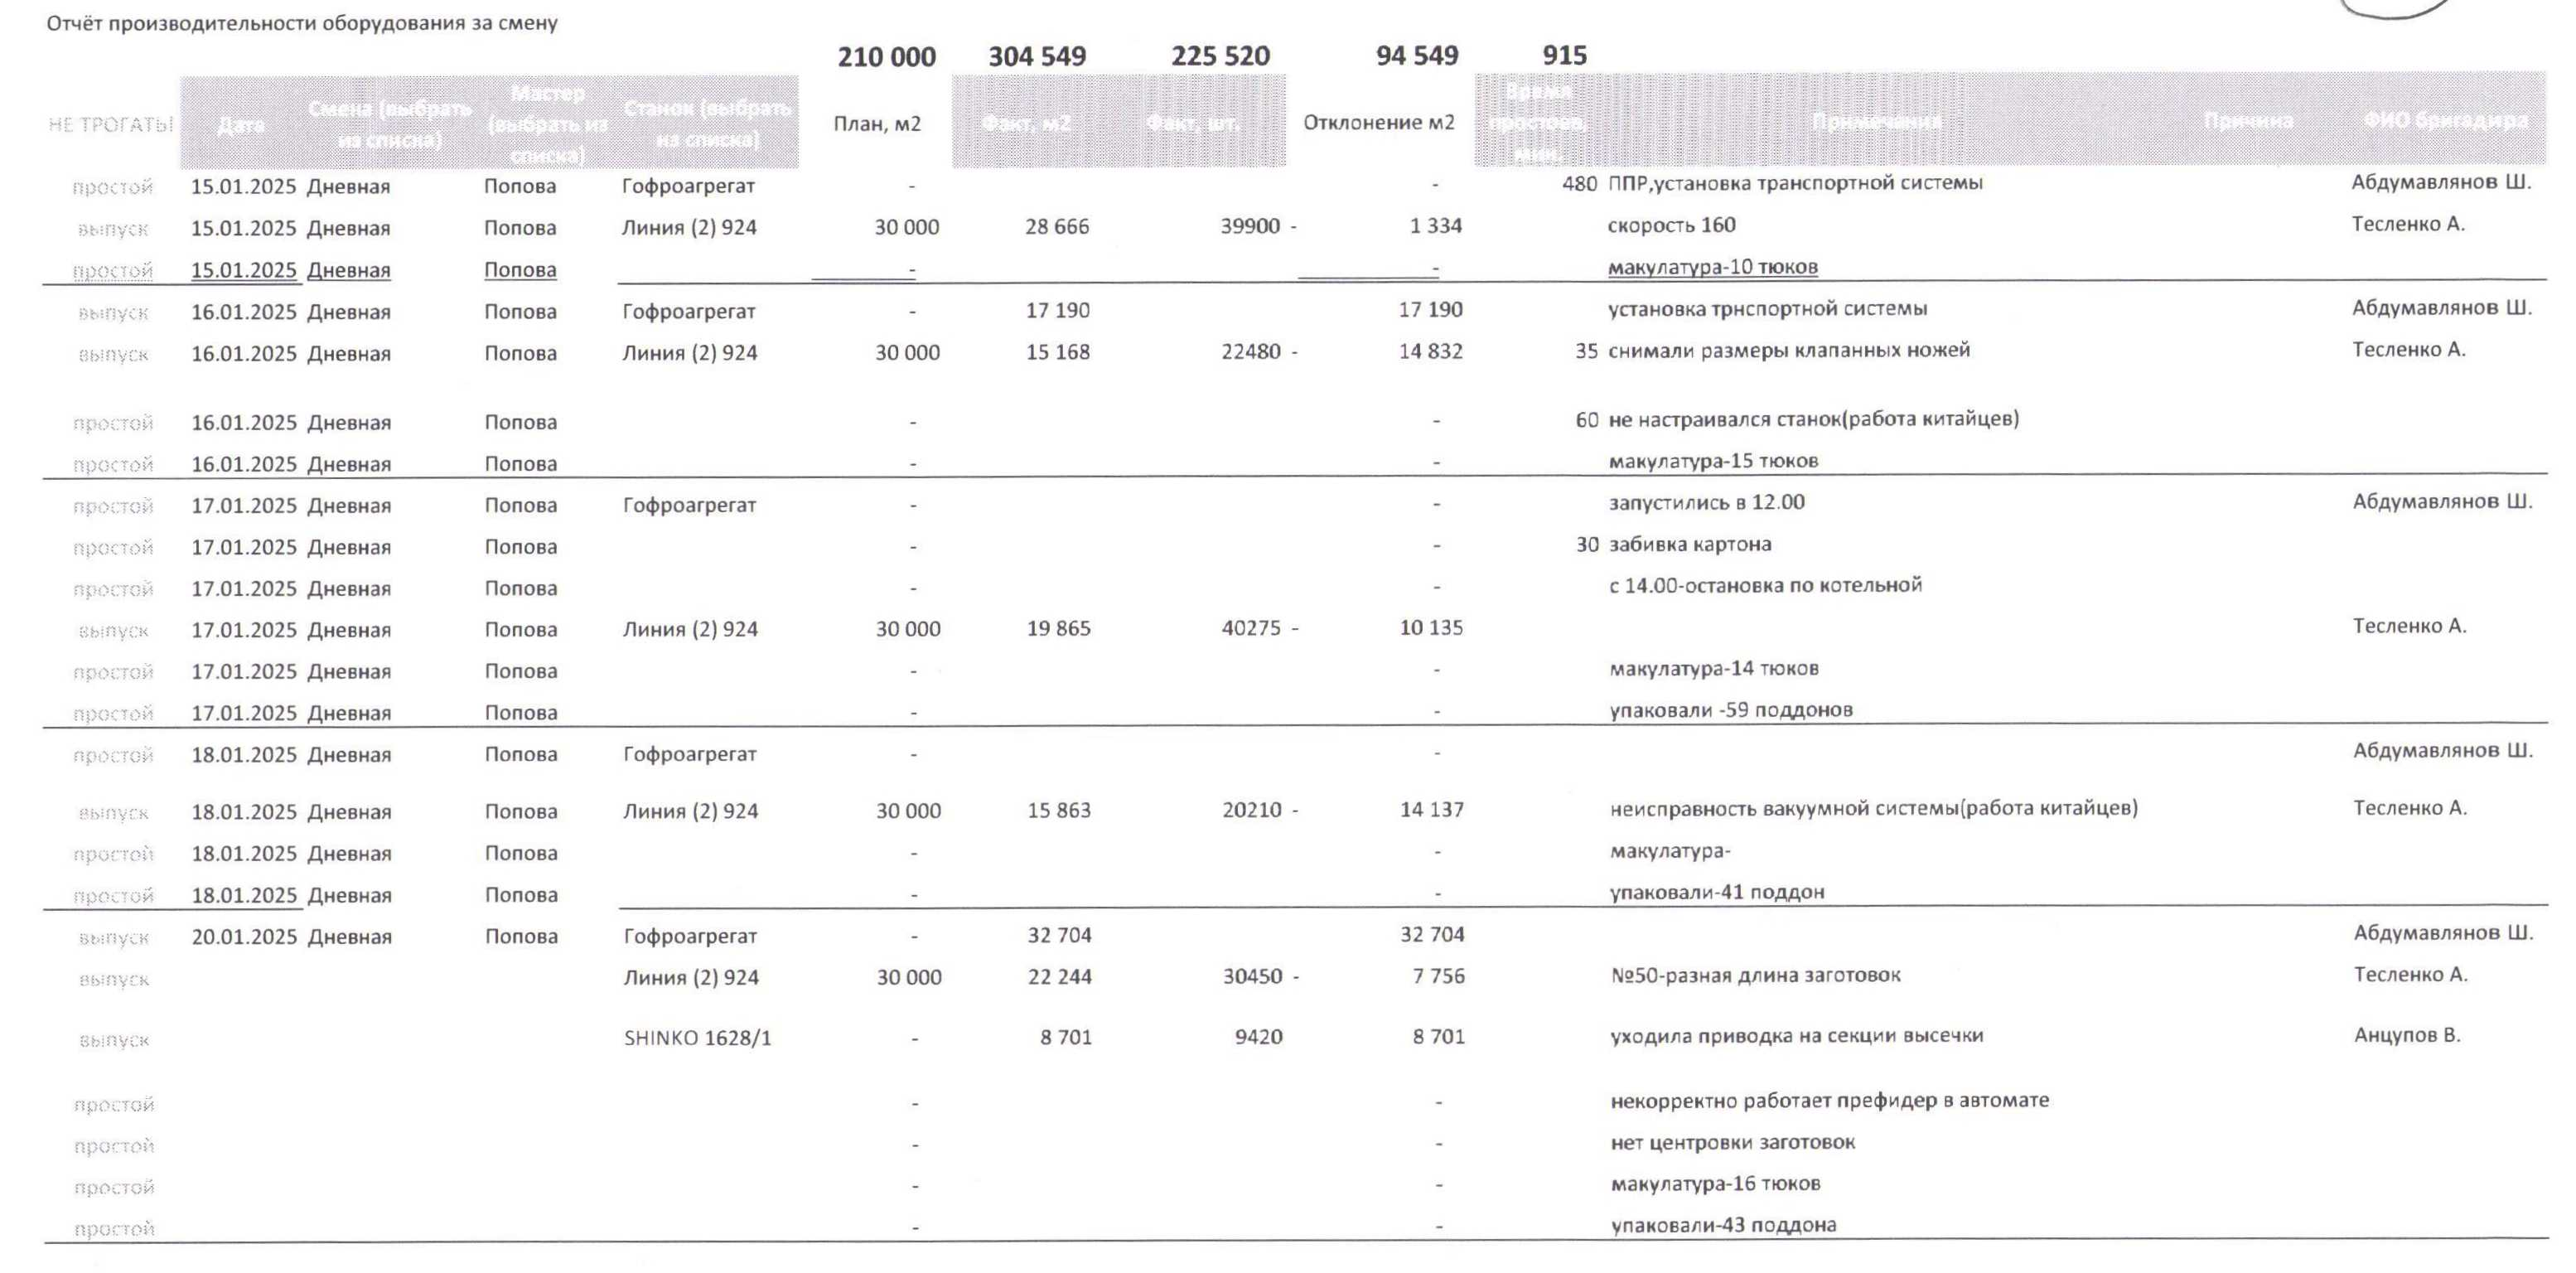
\includegraphics[width=\linewidth, height=0.94\textheight, keepaspectratio]{Pics/f25.jpg}
\end{center}
\caption{Отчет производства за смену ПЛ}
\label{pic:f25}
\end{figure}

\begin{figure}
\begin{center}
 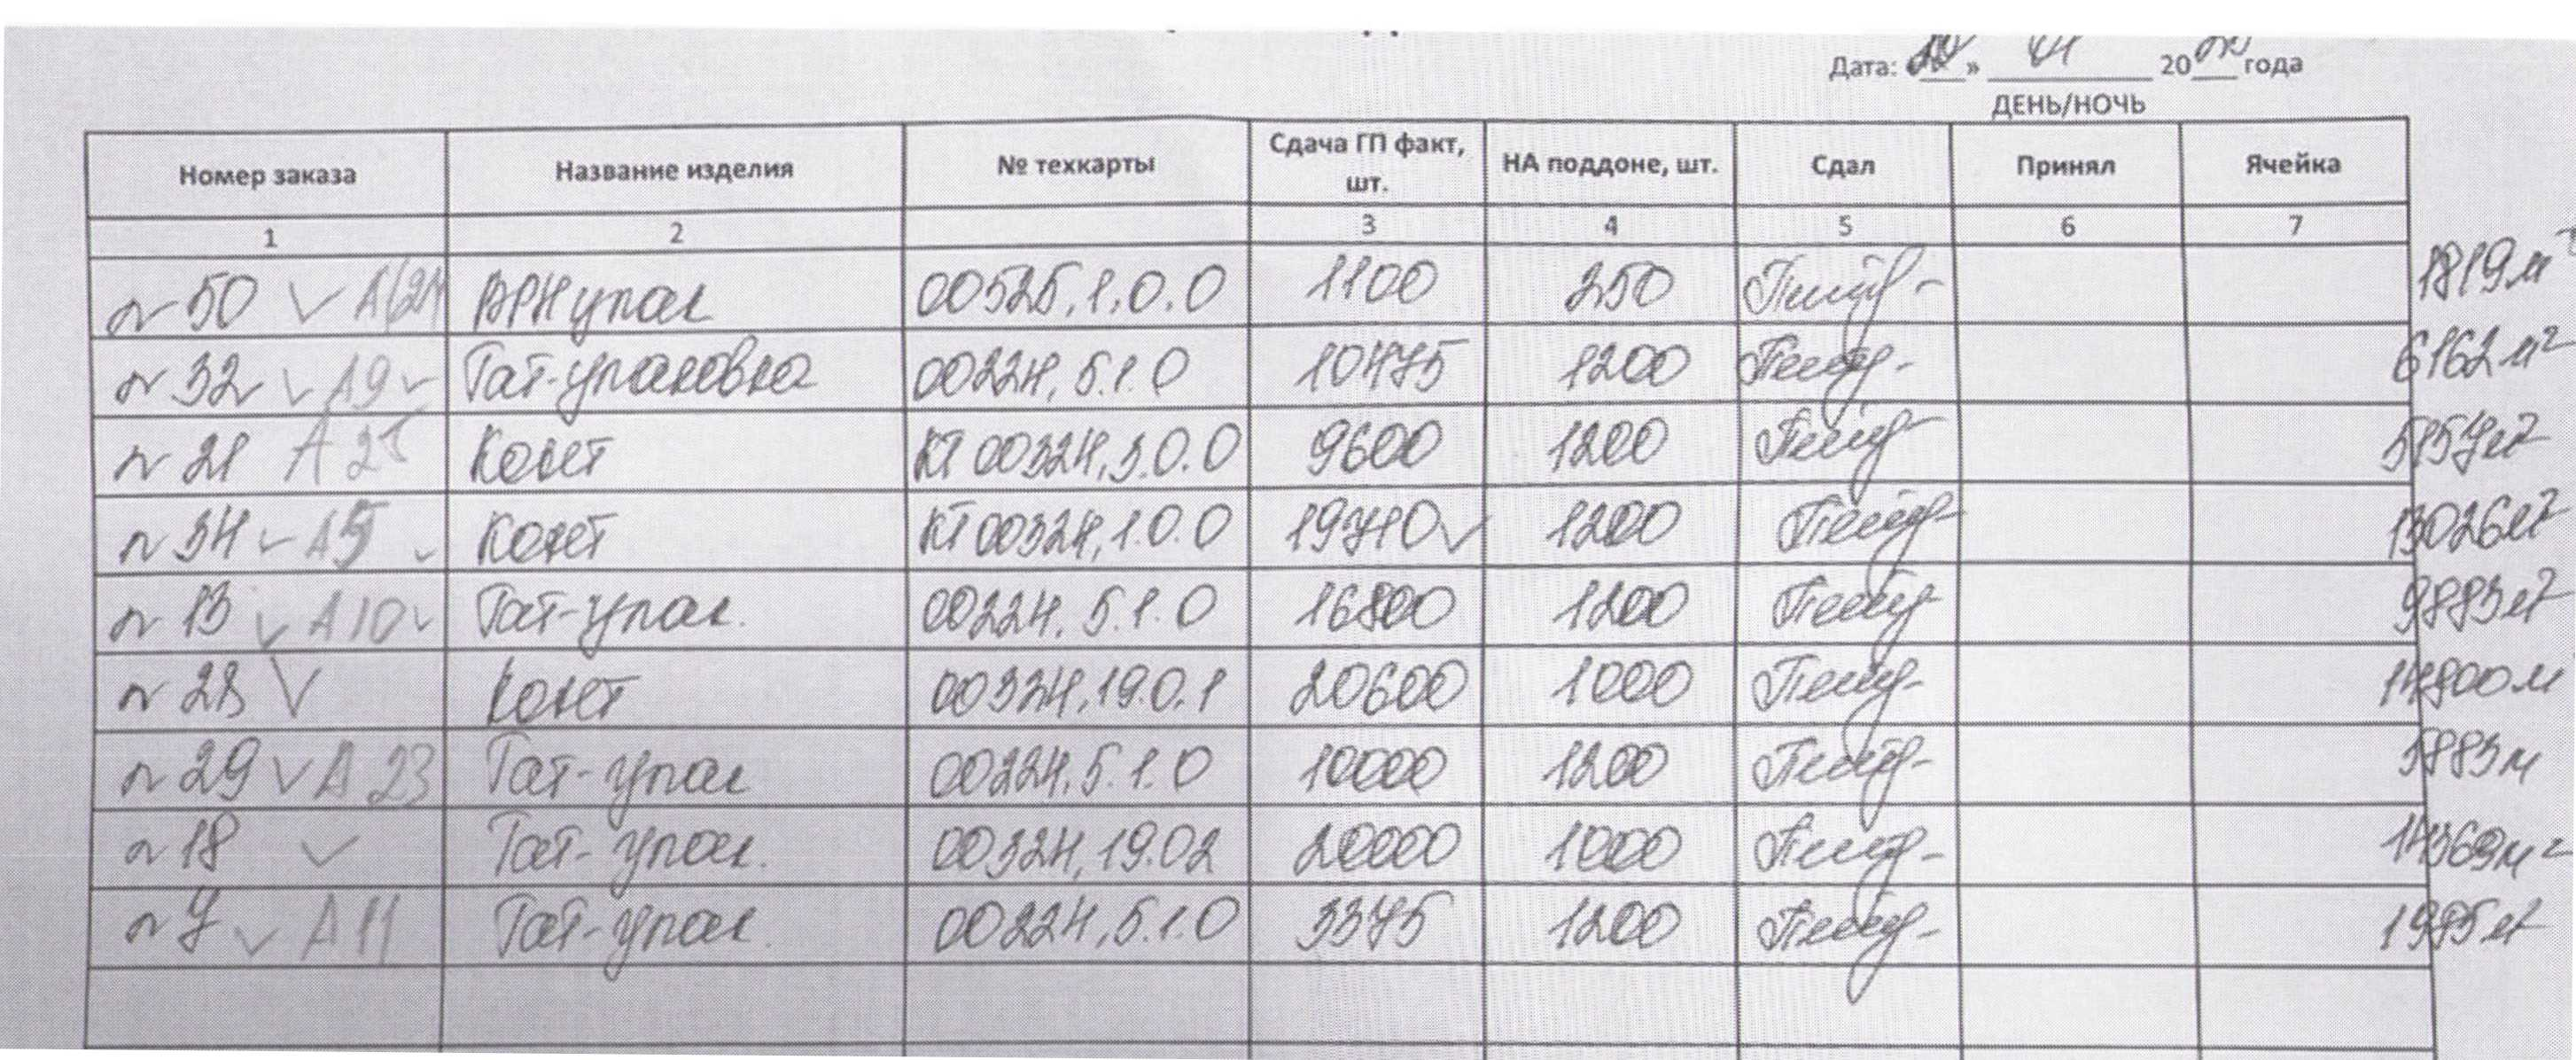
\includegraphics[width=\linewidth, height=0.94\textheight, keepaspectratio]{Pics/f6.jpg}
\end{center}
\caption{Ведомость передачи ГП на склад}
\label{pic:f6}
\end{figure}

\clearpage
% \newpage
\subsection{Изготовление образцов продукции}
\label{bp:pattern}


Процедуры изготовления образцов не выявлено. На момент обследования строилось помещение для плоттера для изготовления образцов. 



\ifx \notincludehead\undefined
\normalsize
\end{document}
\fi
% \newpage
\subsection{Запуск опытной партии}
%

На момент проведения аудита процесс не определен.




\ifx \notincludehead\undefined
\normalsize
\end{document}
\fi

% \newpage
\subsection{Учет отходов производства (макулатуры)}

 

Вся макулатура в виде отходов производства передается в пресс. Прессовщик тюки с  макулатурой складывает в отдельно отведенном месте. Тюки не взвешиваются, на момент обследования не было весов. 

Кладовщик каждый день ведет учет в штуках (тюках).




%\textbf{Учет брака}




\clearpage
\ifx \notincludehead\undefined
\normalsize
\end{document}
\fi
\newpage
\subsection{Учет готовой продукции}
\label{bp:readygoods}


Вся готовая продукция поступает на линию упаковки. Водитель погрузчика забирает паллеты с упакованной готовой продукцией на склад ГП. 

На складе ГП есть разметка для ячеечного хранения продукции (рис. \ref{pic:f5}).

Водитель погрузчика расставляет продукцию на складе в свободные ячейки и указывает в ведомости параметры продукции и ячейку, куда поставил ГП (рис. \ref{pic:f7}). В конце смены ведомость передается кладовщику. Кладовщик вносит данные в таблицу MS EXCEL (рис. \ref{pic:f10}).

В конце смены мастер смены заполняет свою ведомость по данным работы производственной  линий (рис. \ref{pic:f6}). По этой ведомости мастер сверяется с данными подаваемыми кладовщиком и подтверждают факт подписями. 


\begin{figure}
\begin{center}
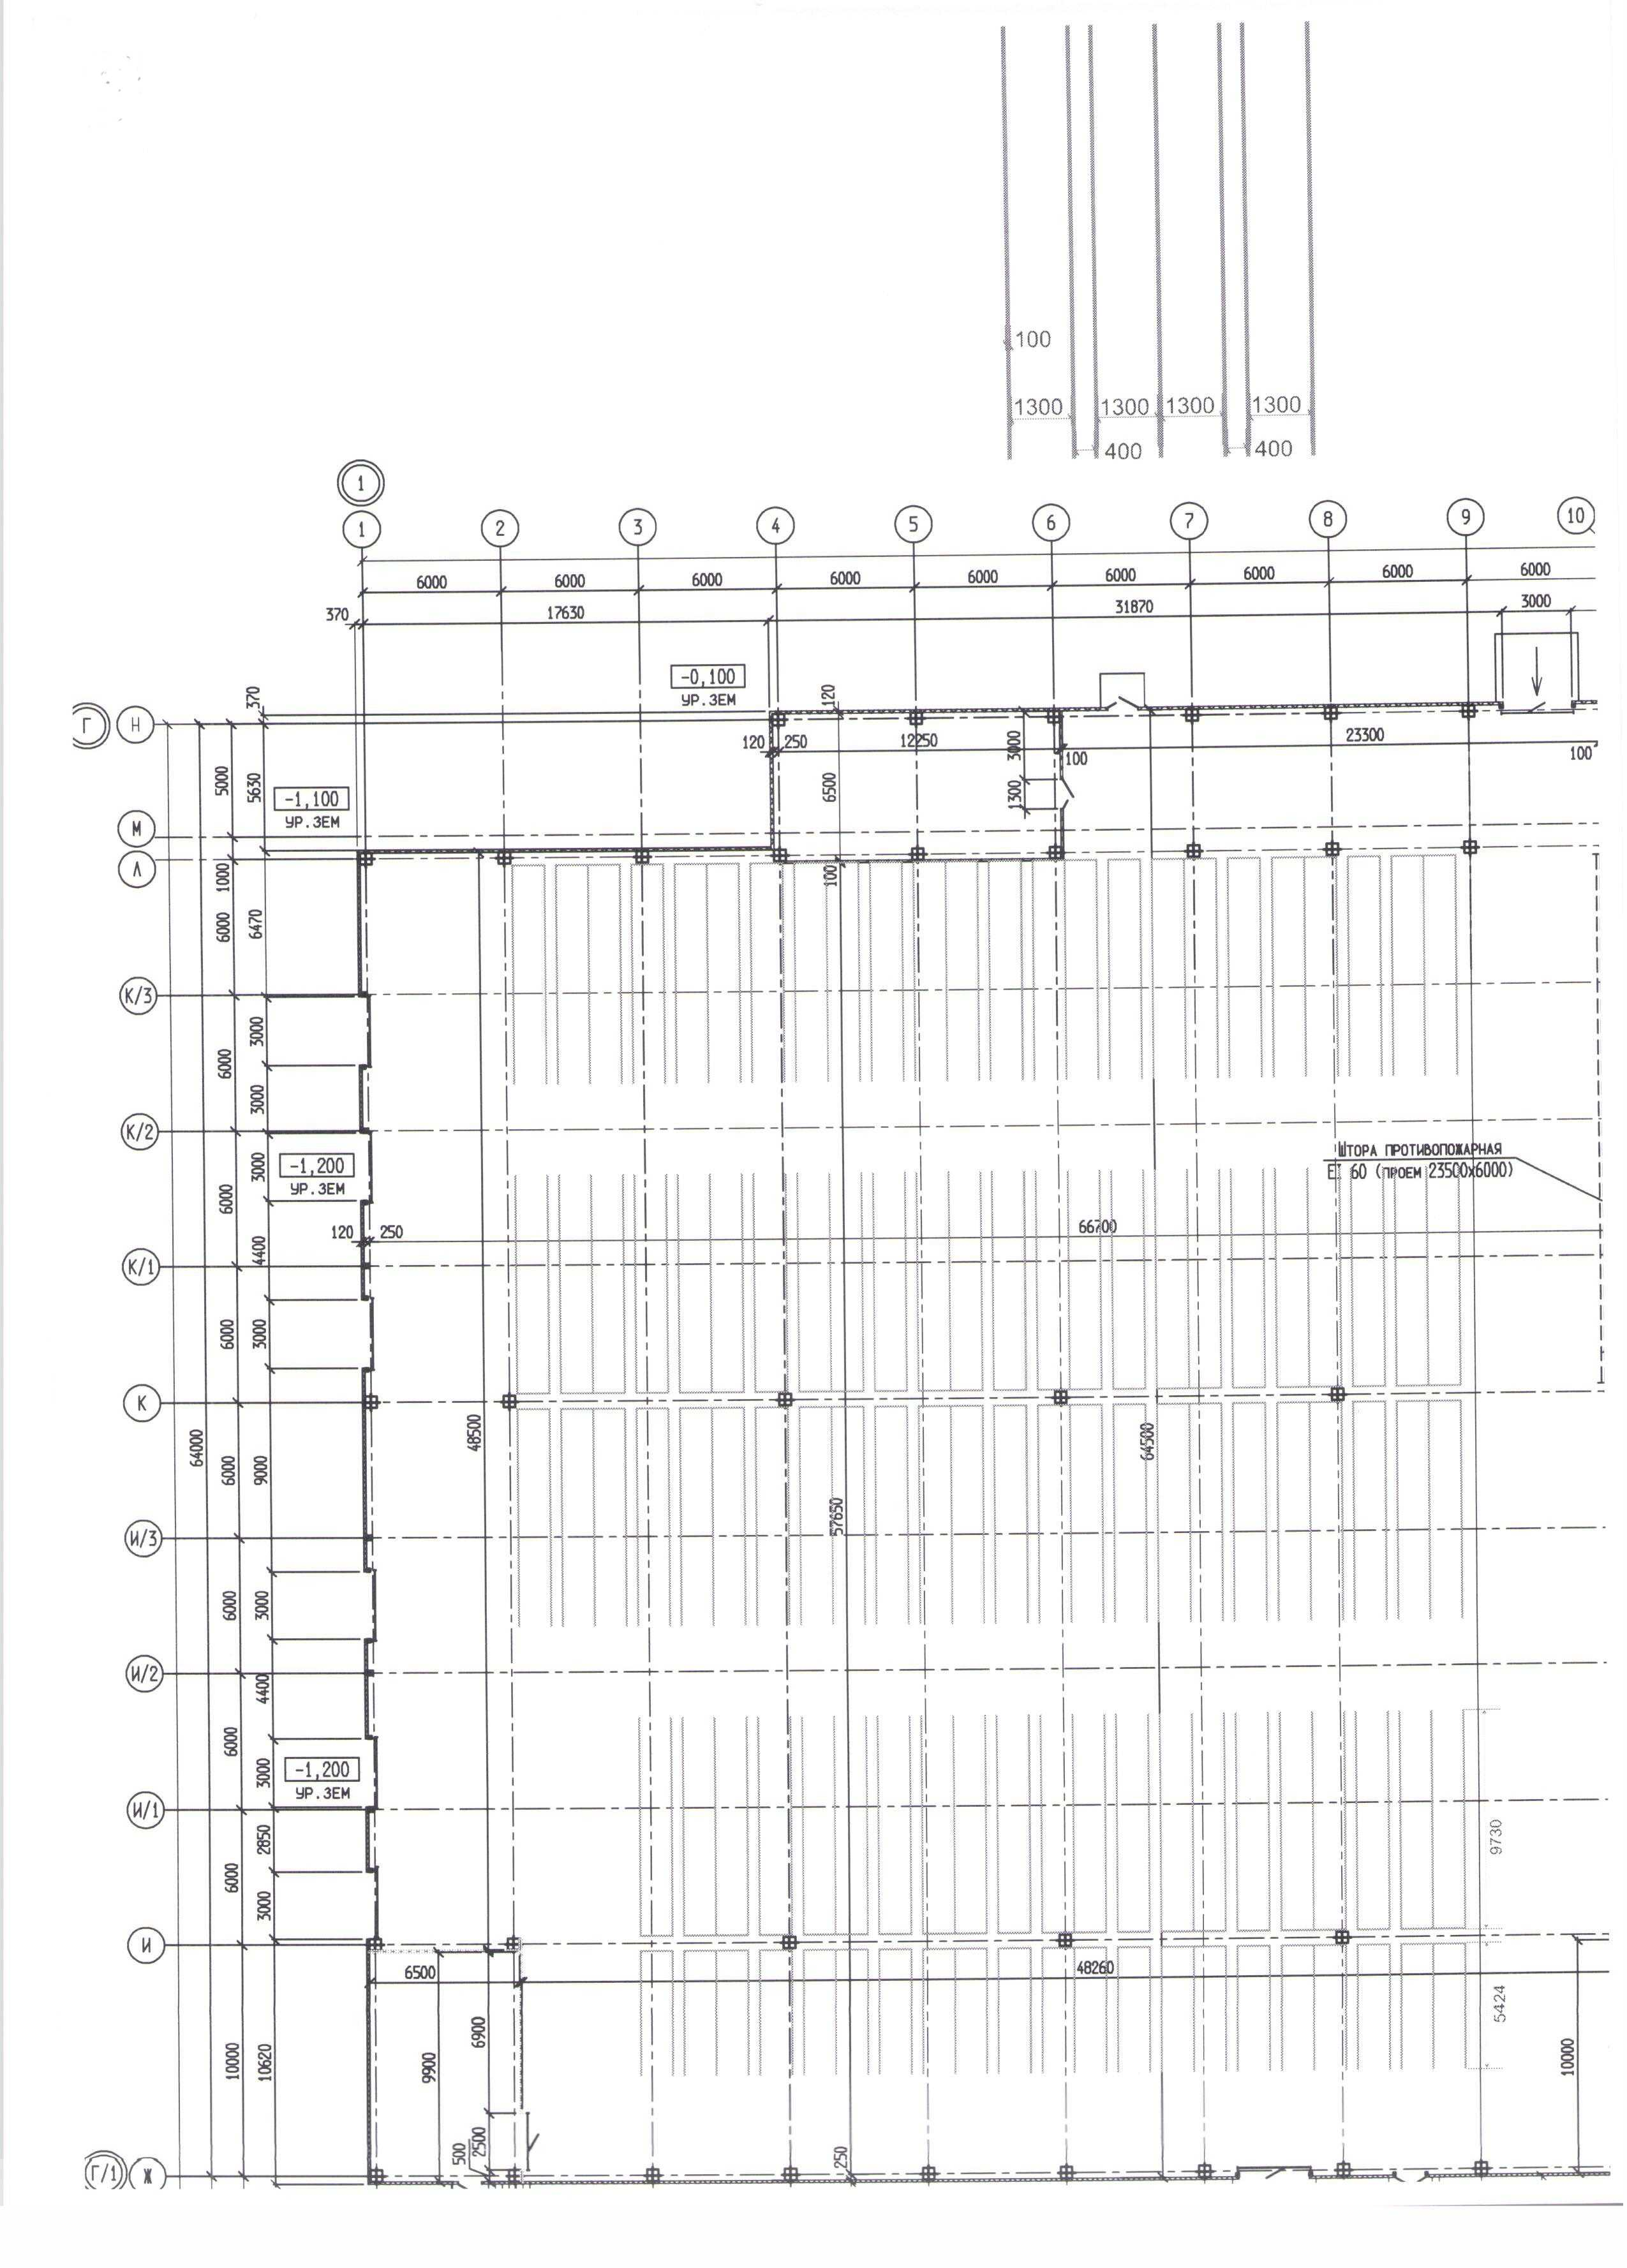
\includegraphics[height=0.94\textheight, width=\textwidth, keepaspectratio]{Pics/f5.jpg}
\end{center}
\caption{Склад ГП. Разметка предусматривающая ячеистое хранение продукции}
\label{pic:f5}
\end{figure}


\begin{figure}
\begin{center}
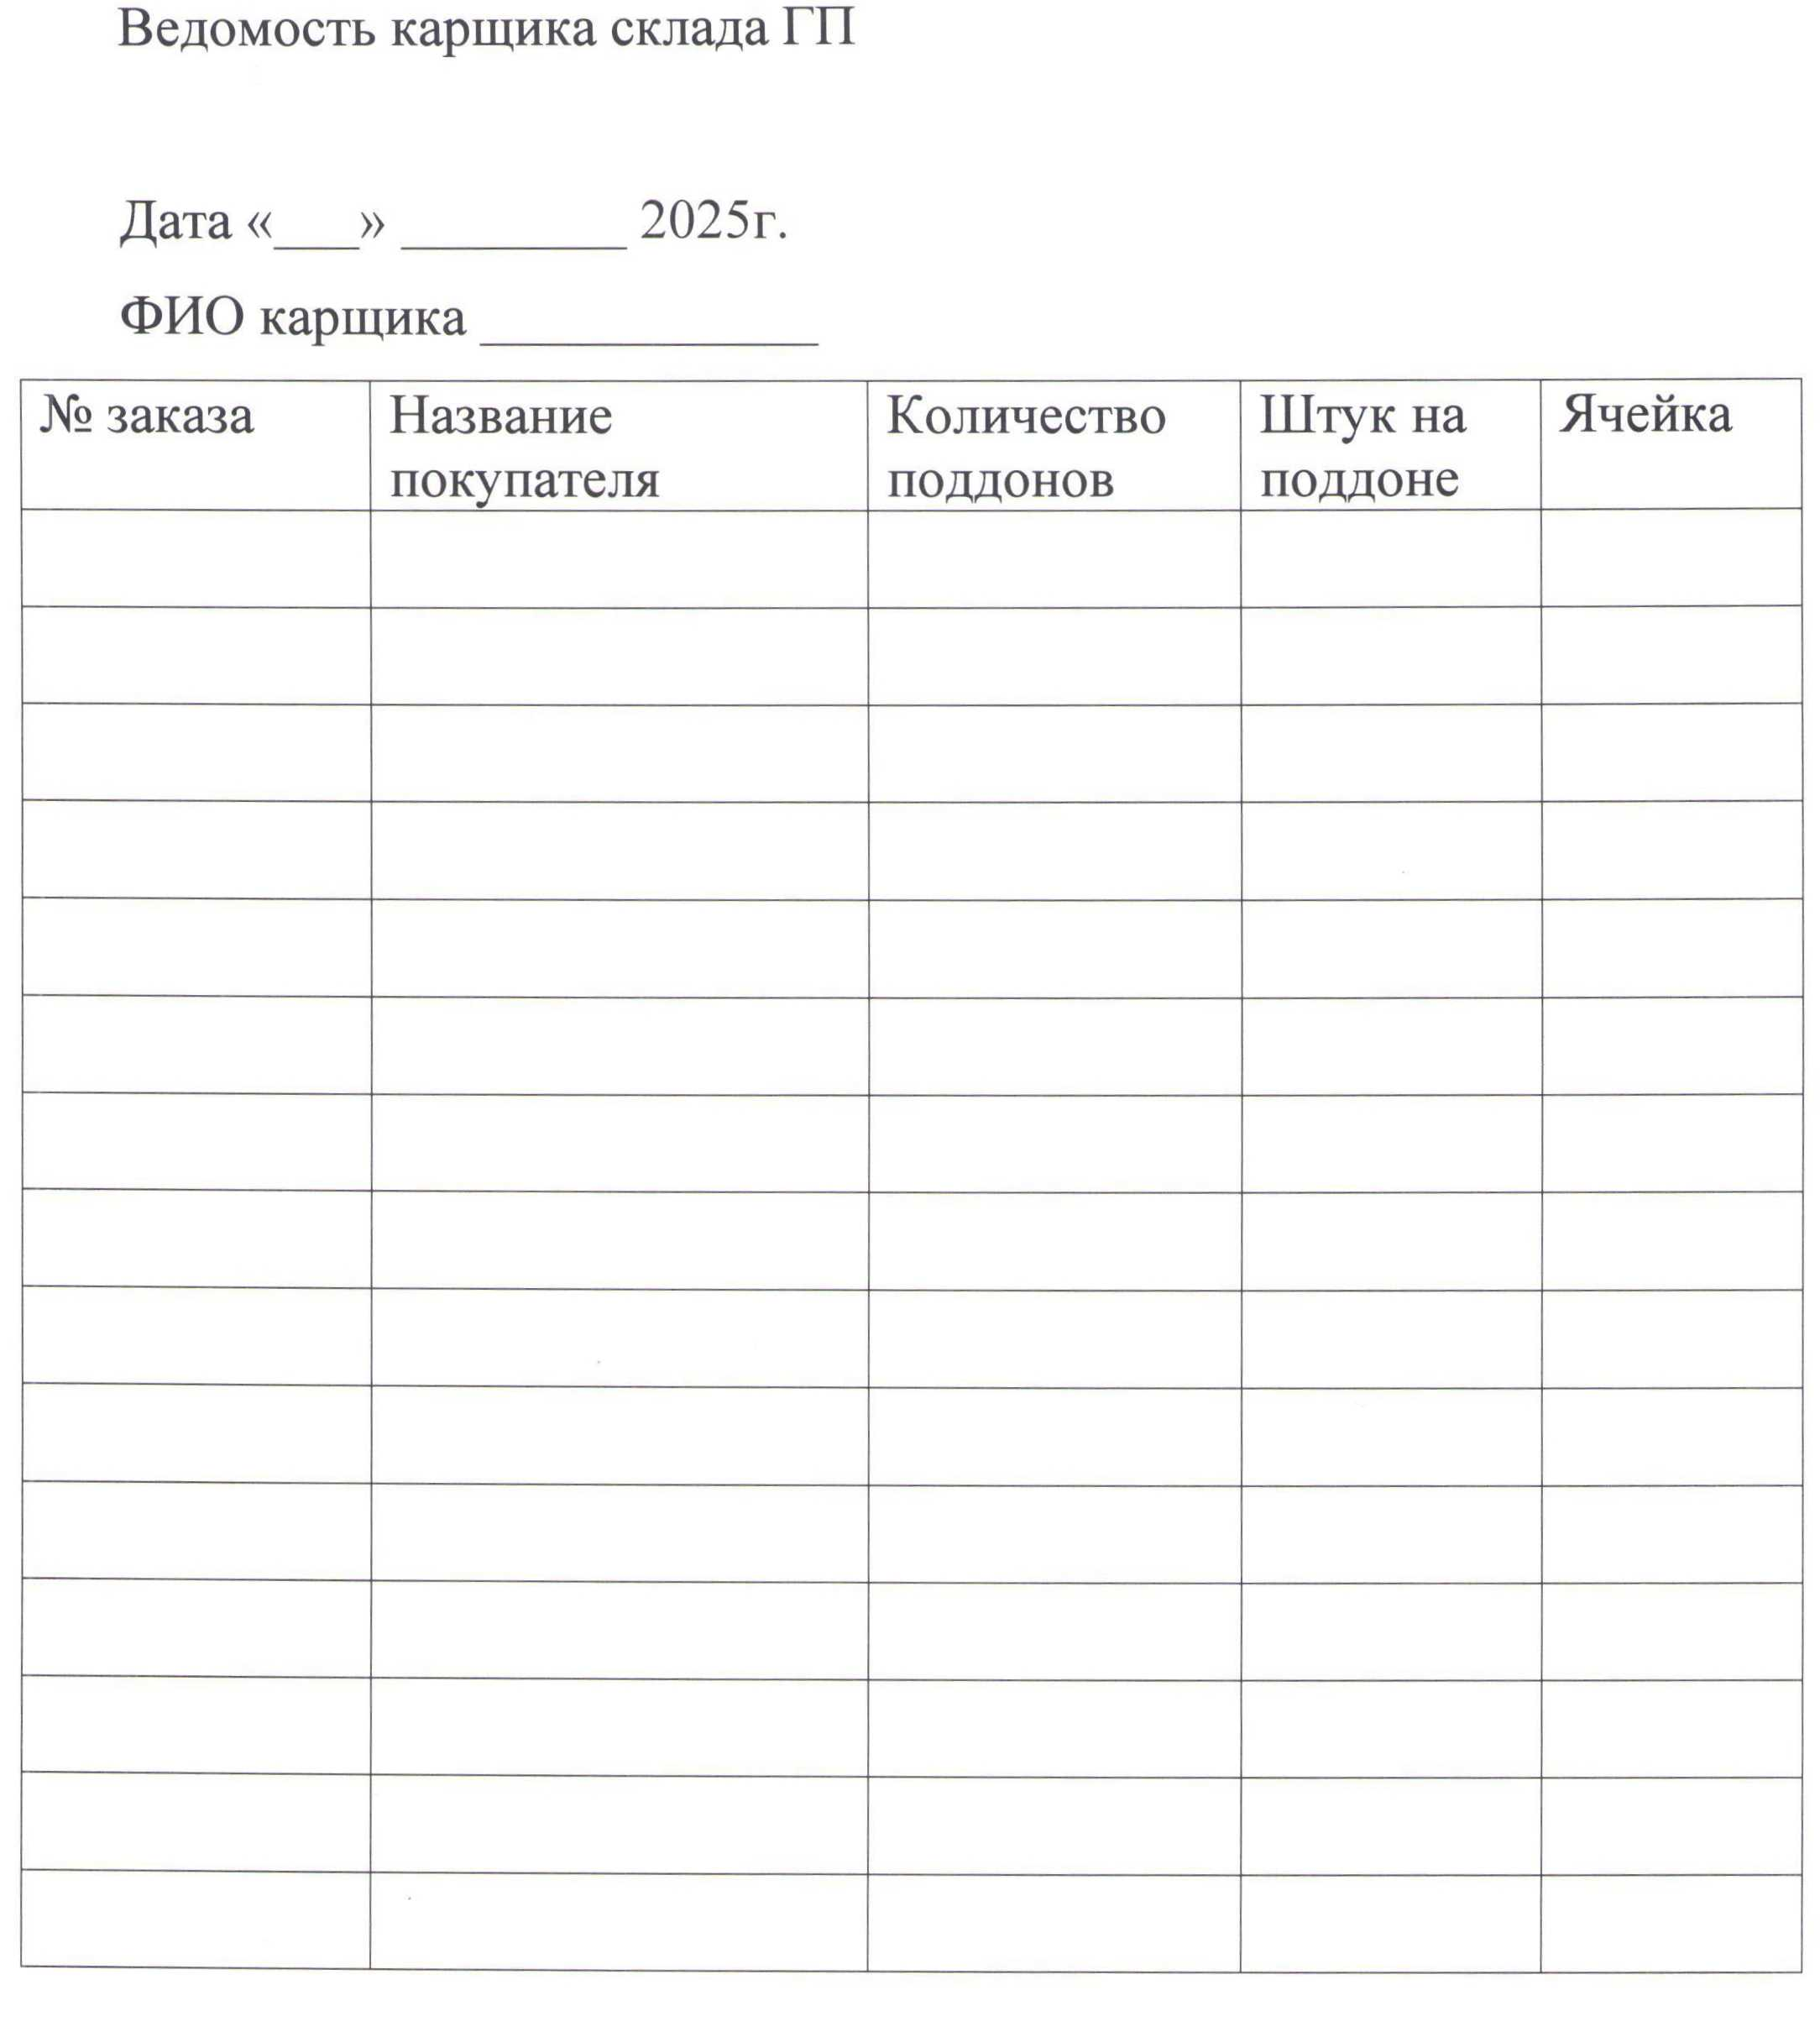
\includegraphics[height=0.94\textheight, width=\textwidth, keepaspectratio]{Pics/f7.jpg}
\end{center}
\caption{Ведомость карщика склада ГП}
\label{pic:f7}
\end{figure}


\newpage
\subsection{Поступление материалов}
\label{bp:MatInput}
%


\subsubsection{Поступление бумаги и картона}

Рулоны бумаги и картона принимаются кладовщиками на склад ролевой продукции. 

Сырье транспортируется машинами. При срочной необходимости могут с предприятия <<Эколайнер>>  привезти автопогрузчиком необходимый рулон. 

Сырье с <<Эколайнер>> поступает по актам передачи (рис. \ref{pic:f13}). Их подписывают кладовщики. Сырье других поставщиков приходит с обычным пакетом документов. 

При поступлении сырья на склад кладовщик сверяет данные, указанные на маркировочных этикетках рулонов с сырьем, с данными, указанными в документах (рис. \ref{pic:f9}), вносит данные в таблицу MS EXCEL (рис. \ref{pic:f1}), где ведется основной учет. 

Основные документы сразу поступают в бухгалтерию.





% \subsubsection{Поступление рулонов бумаги и картона}

% Не производится.




\subsubsection{Поступление прочих материалов}

На момент обследования все вспомогательные материалы числятся на складе другого завода.



\begin{figure}
\begin{center}
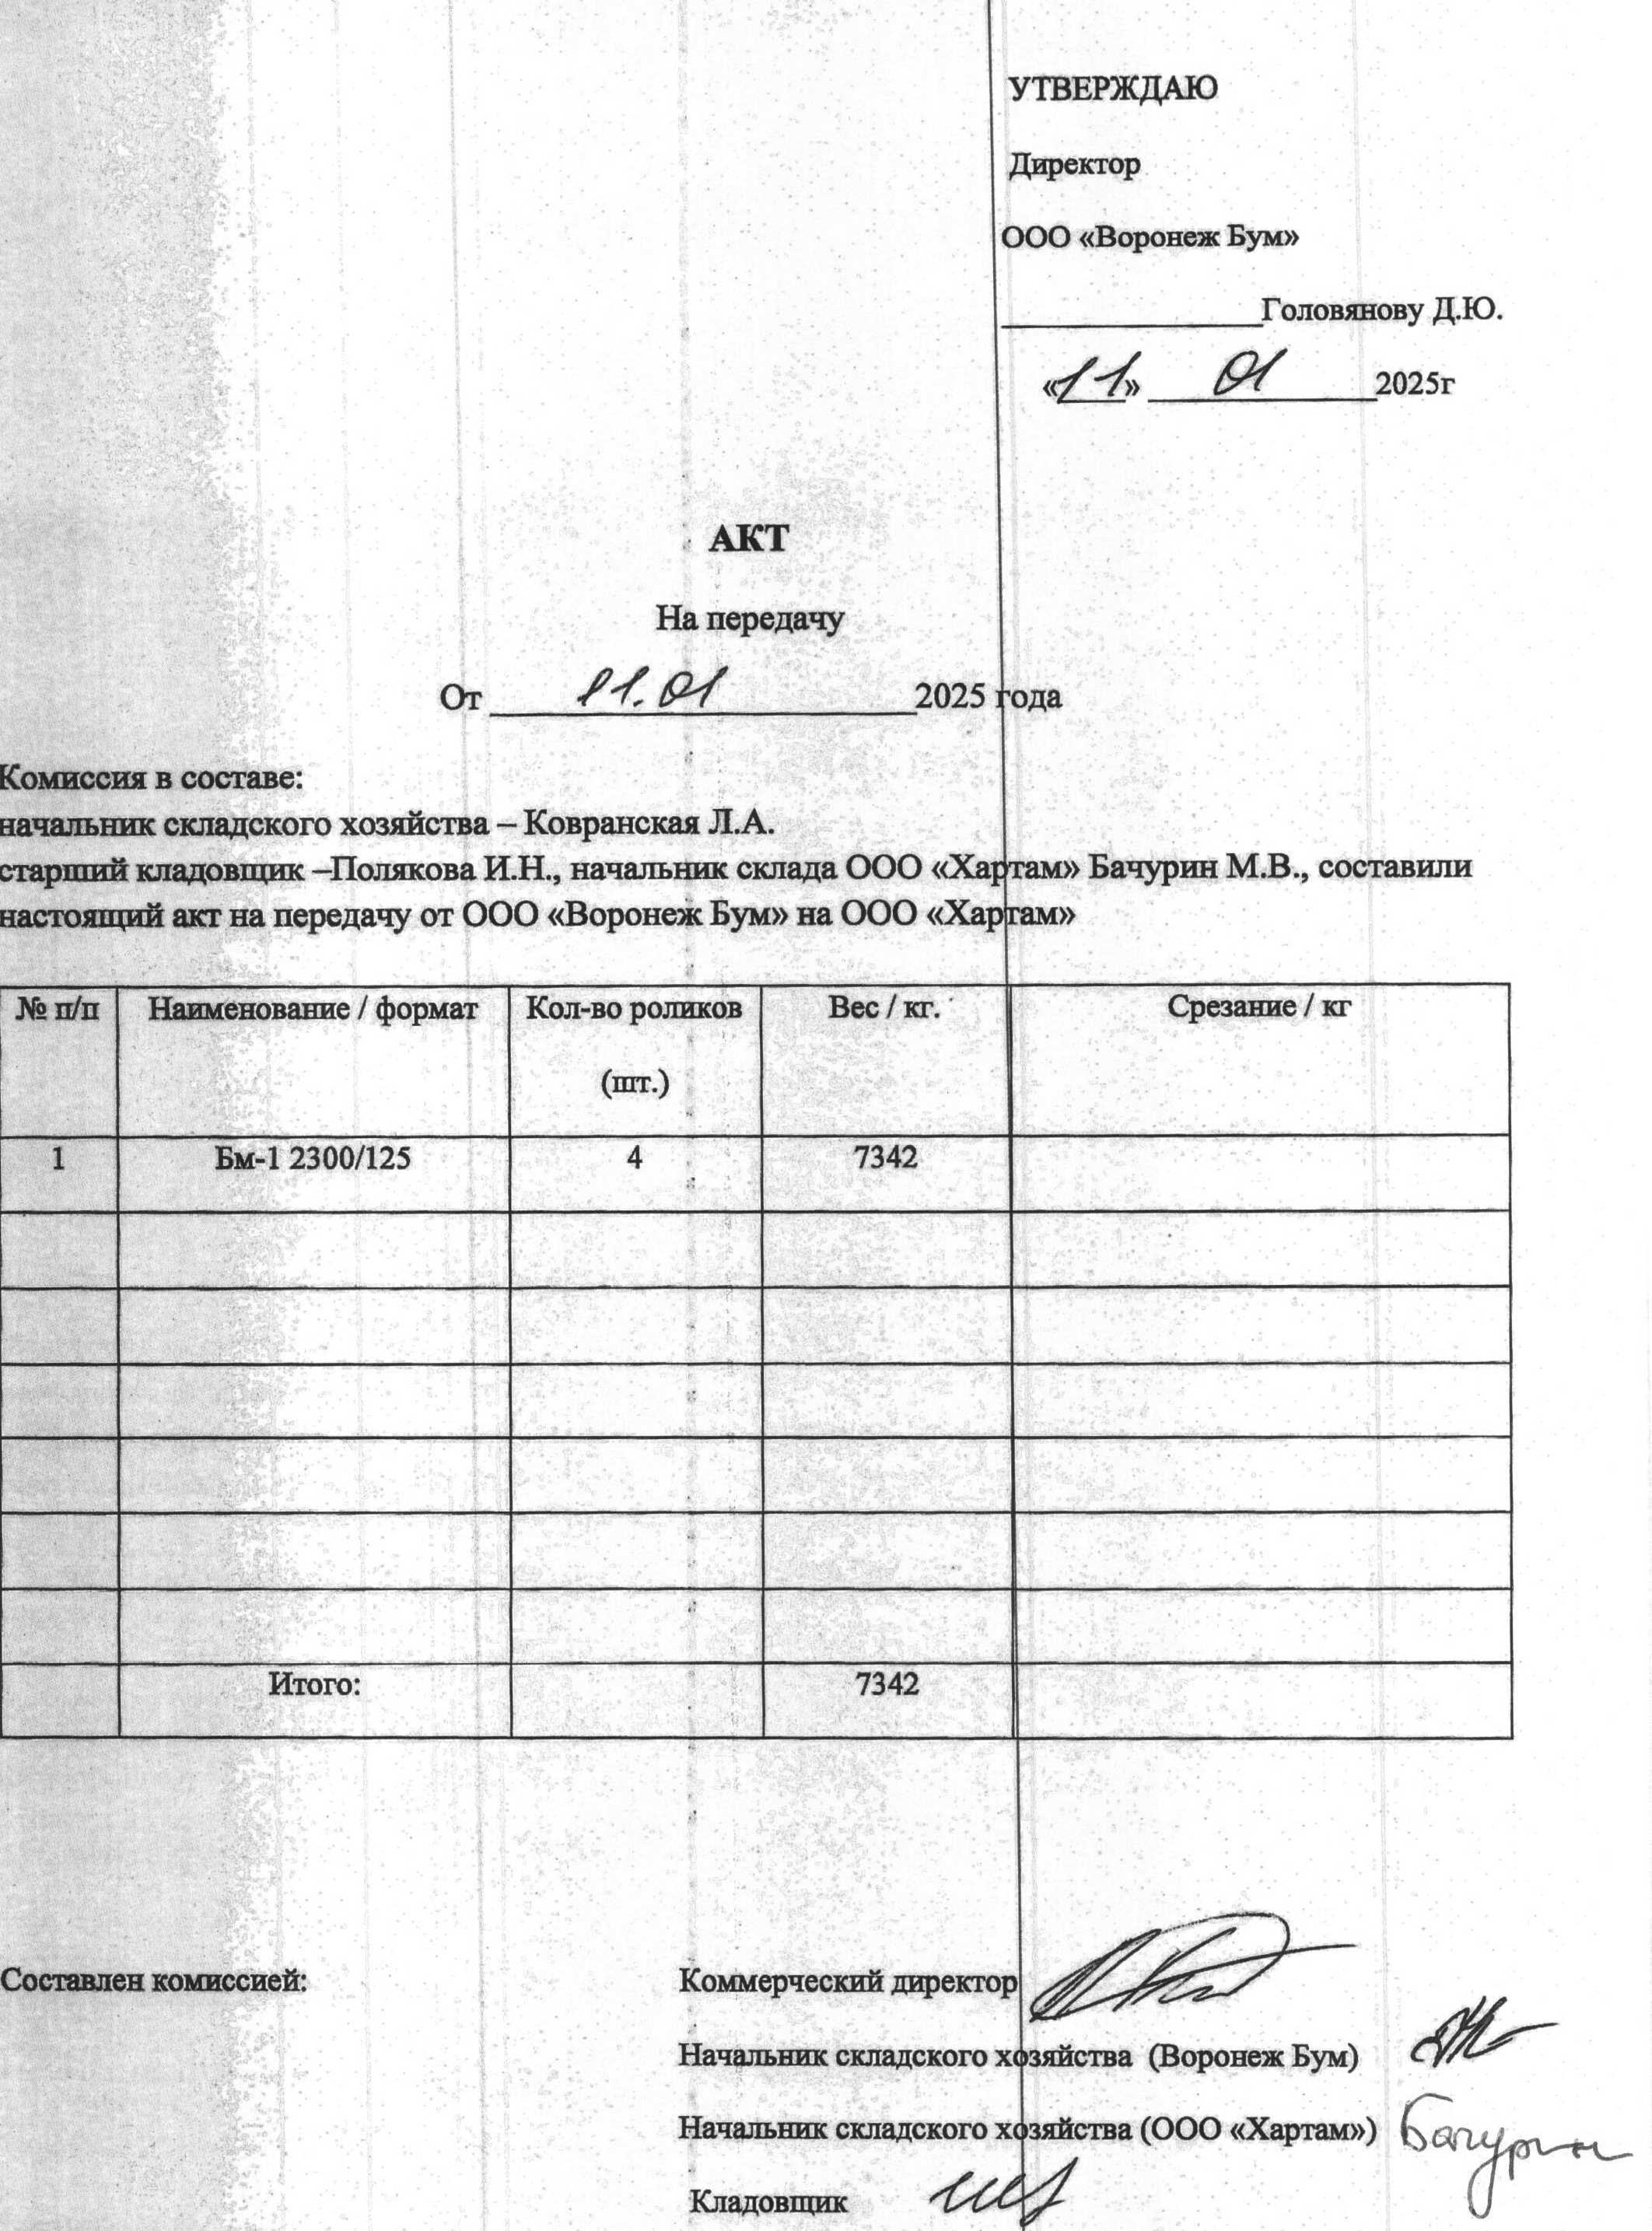
\includegraphics[height=0.94\textheight, width=\textwidth, keepaspectratio]{Pics/f13.jpg}
\end{center}
\caption{Акт на передачу}
\label{pic:f13}
\end{figure}

\begin{figure}
\begin{center}
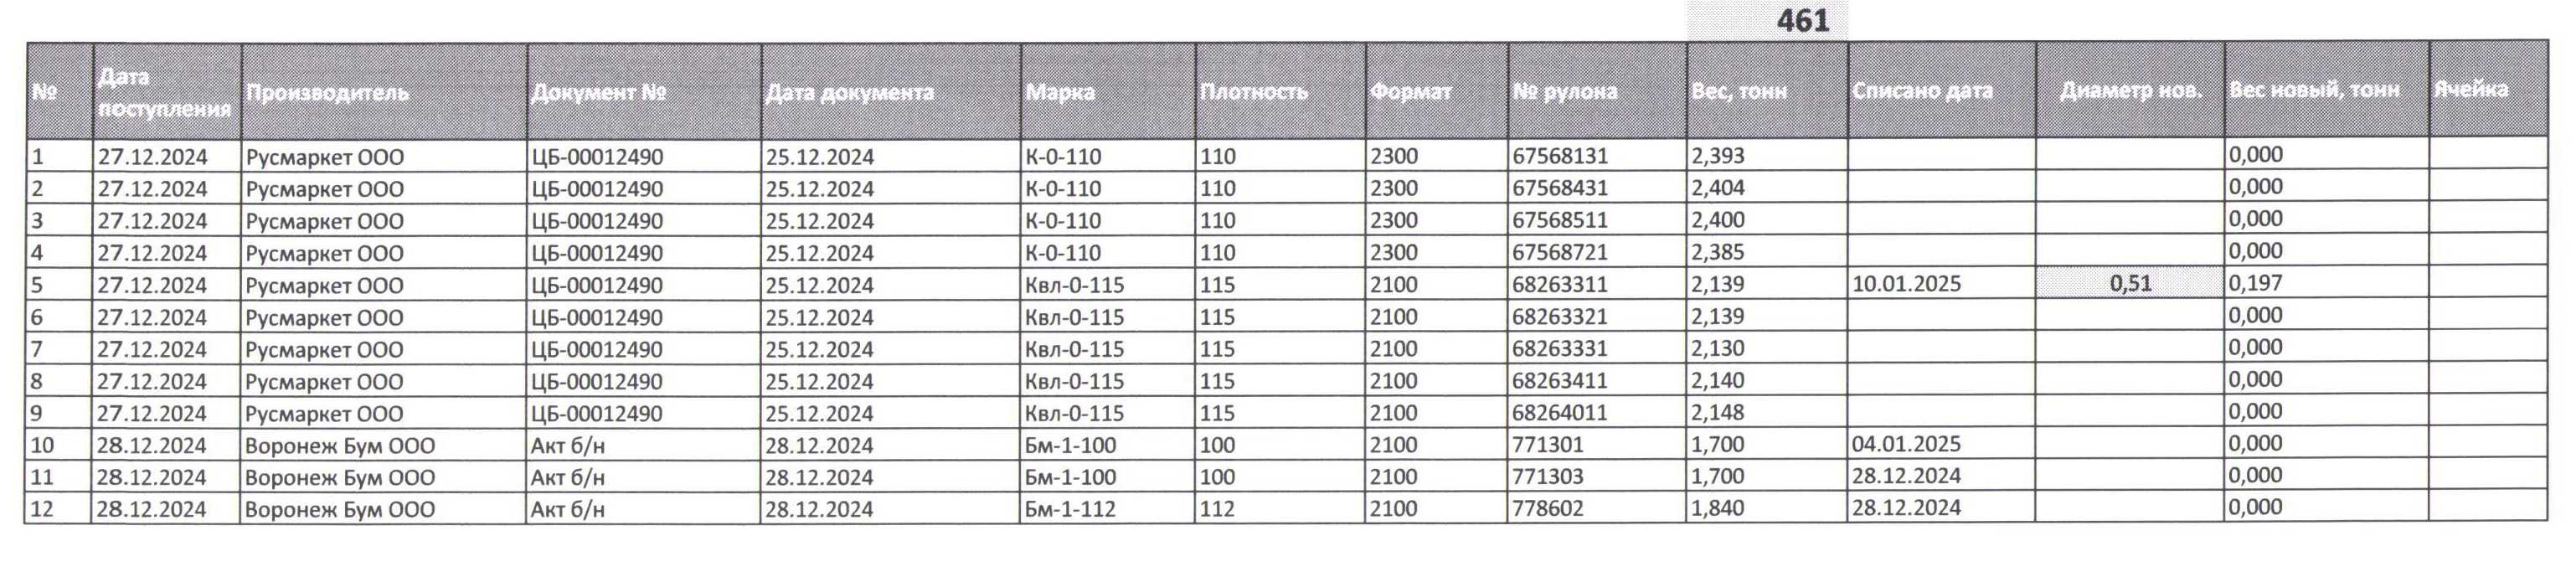
\includegraphics[height=0.94\textheight, width=\textwidth, angle=90, keepaspectratio]{Pics/f1.jpg}
\end{center}
\caption{По рулонный учет сырья}
\label{pic:f1}
\end{figure}

\begin{figure}
\begin{center}
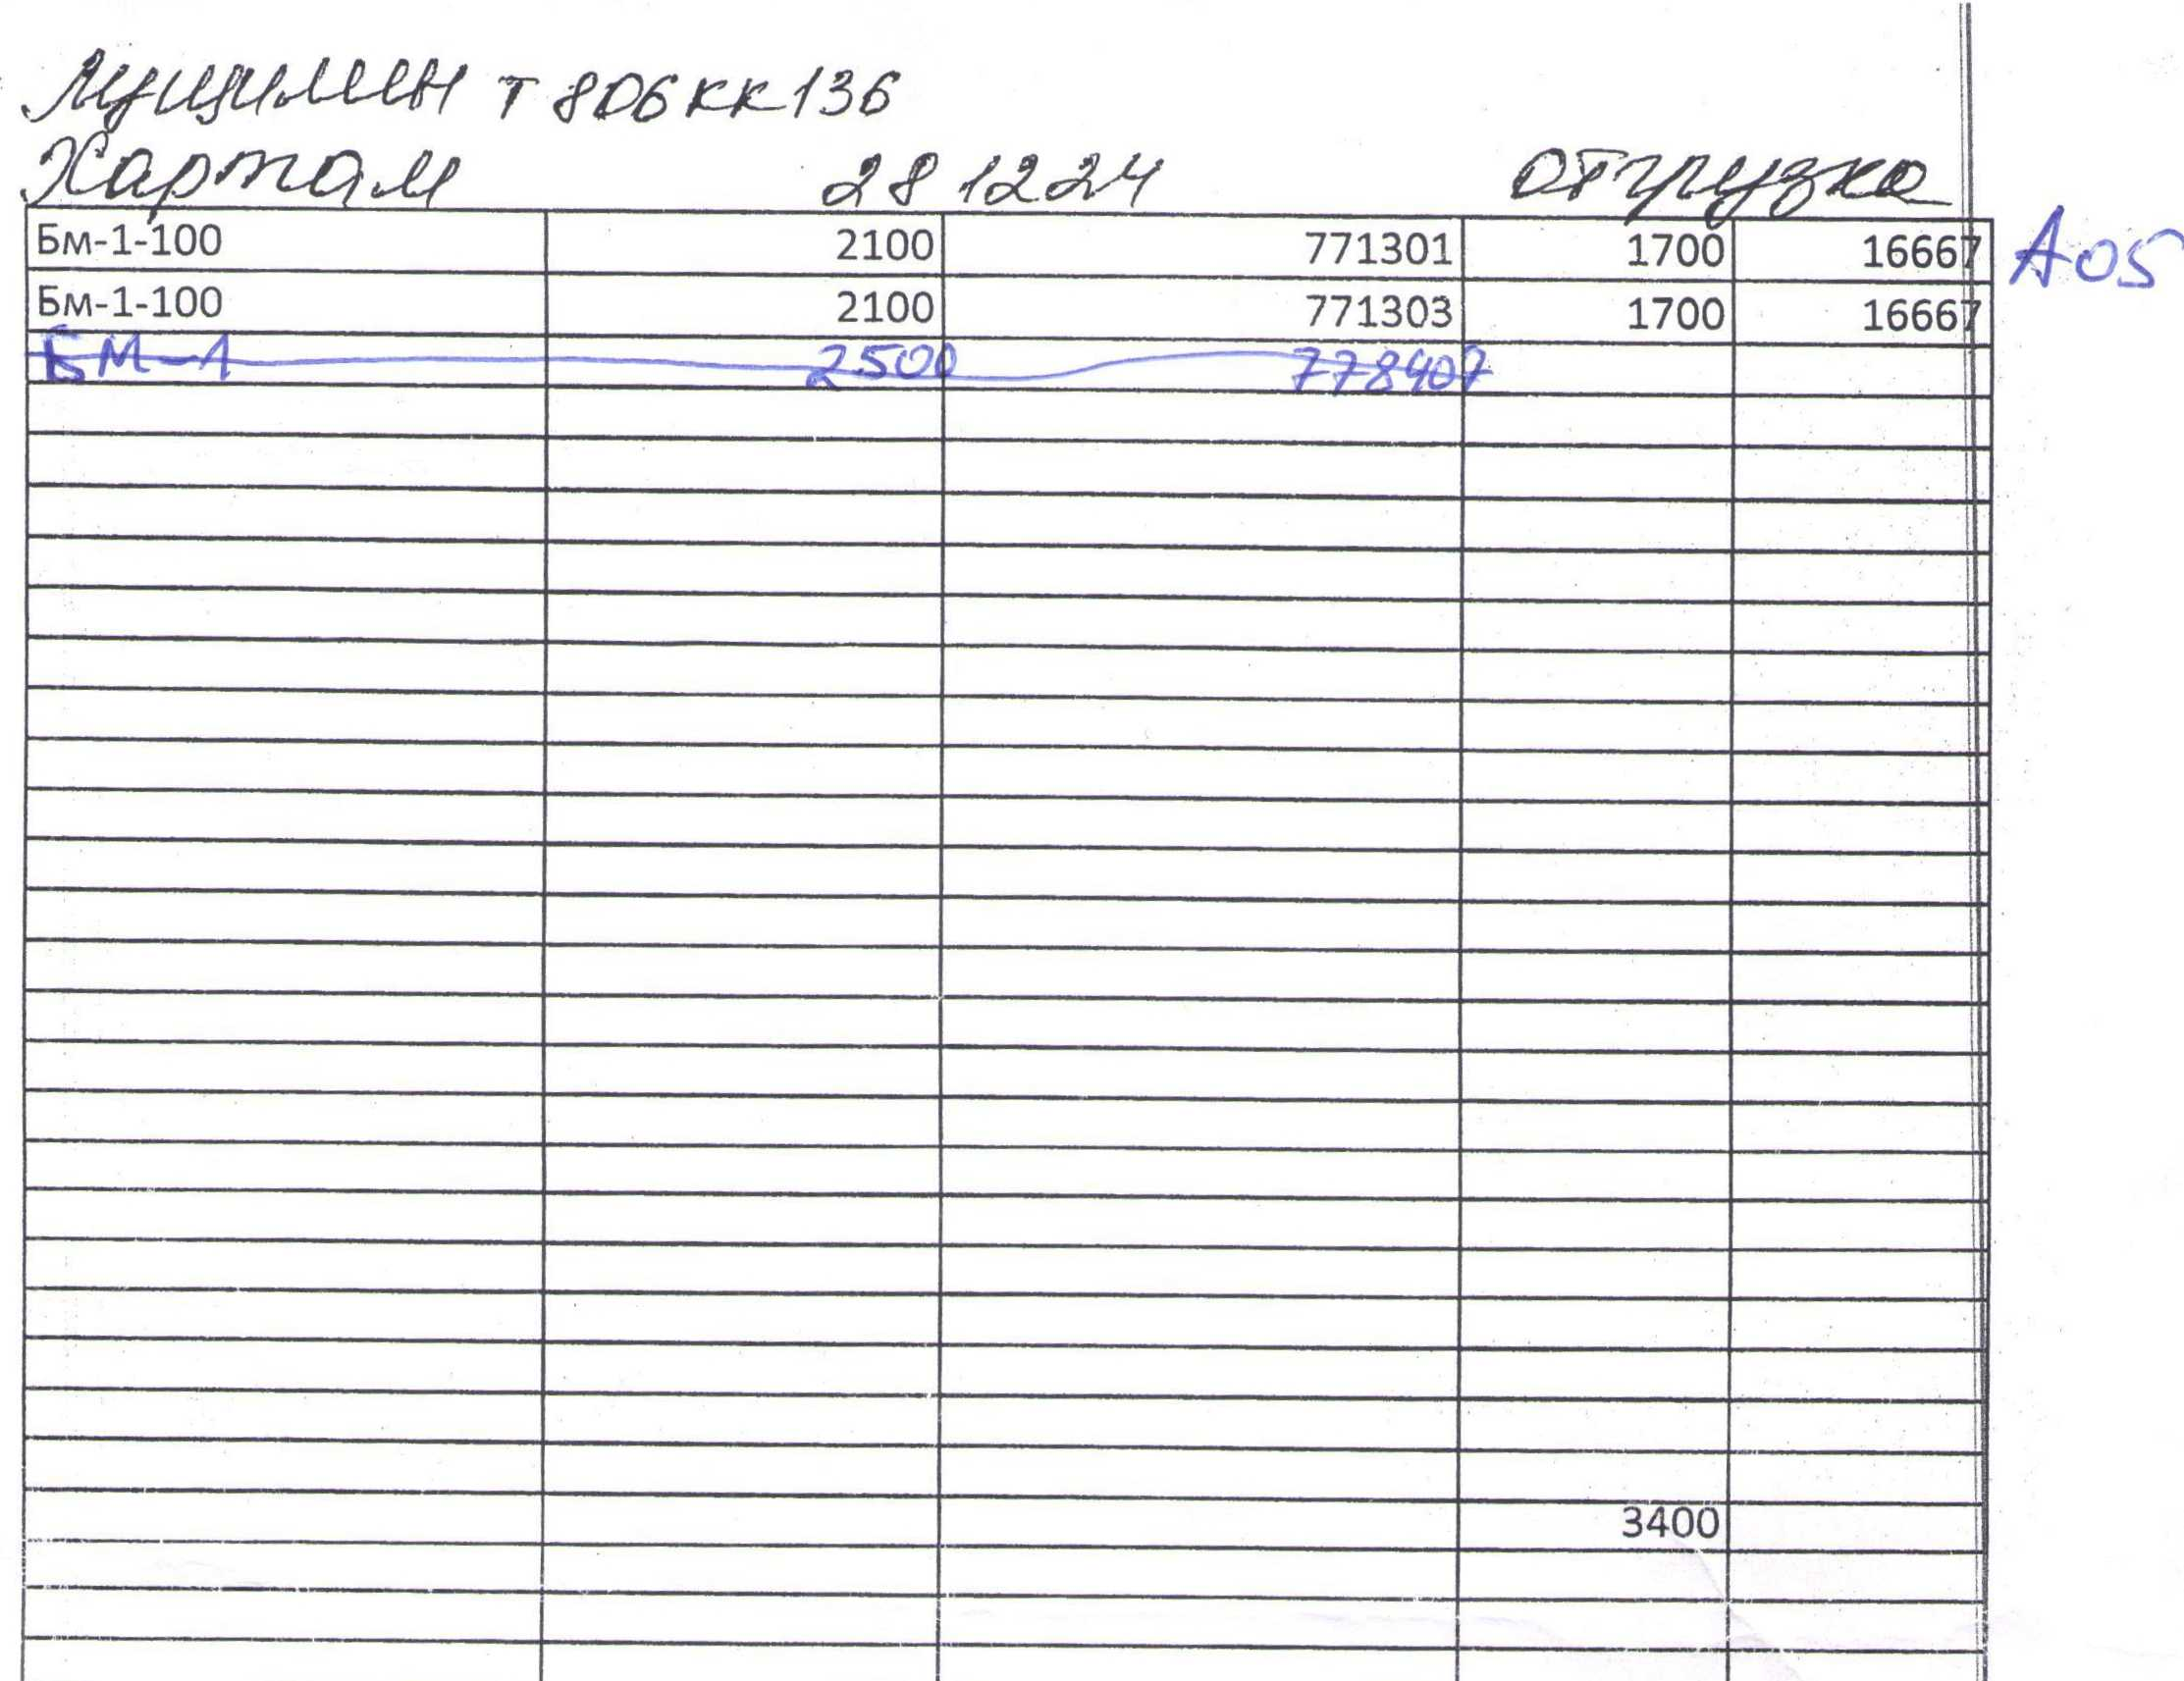
\includegraphics[height=0.94\textheight, width=\textwidth, angle=90, keepaspectratio]{Pics/f9.jpg}
\end{center}
\caption{Отвес сырья}
\label{pic:f9}
\end{figure}


\clearpage
\ifx \notincludehead\undefined
\normalsize
\end{document}
\fi
\newpage
%
\subsection{Списание материалов}
\label{bp:MatOutput}

\subsubsection{Списание бумаги и картона}


Бригадир ГА получает плановое задание на гофроагрегат (рис. \ref{pic:f8b} - \ref{pic:f8a}),
определяет потребность в сырье, в устной форме передает ее кладовщику. Кладовщик с водителем погрузчика находят необходимое сырье и подают на гофроагрегат.

Сырьевые остатки в виде частично использованных рулонов обратно на склад не возвращаются. Учет частично использованных рулонов ведется производством в штуках, а не в килограммах (отсутствуют весы).

Все переданное на производство сырье кладовщик вносит в таблицу MS EXCEL с указанием даты передачи.

Кладовщик ведет ведомость списания сырья, которую подписывает бригадир, и передает ее в бухгалтерию (рис. \ref{pic:f26}).

Все остатки формируются ежедневно в таблице MS EXCEL (рис. \ref{pic:f2}).

На складе сырья планируется выполнить разметку для ячеечного хранения продукции (рис. \ref{pic:f4}). 




\subsection{Учет вспомогательных материалов}

Каждый день кладовщик сверяет остатки ТМЦ на складе с данными таблицы MS EXCEL (рис. \ref{pic:f2}) и вносит необходимые корректировки.

Деревянные поддоны учитываются отдельно и выдаются на производство по ведомости  (рис. \ref{pic:f27}).





\begin{figure}
\begin{center}
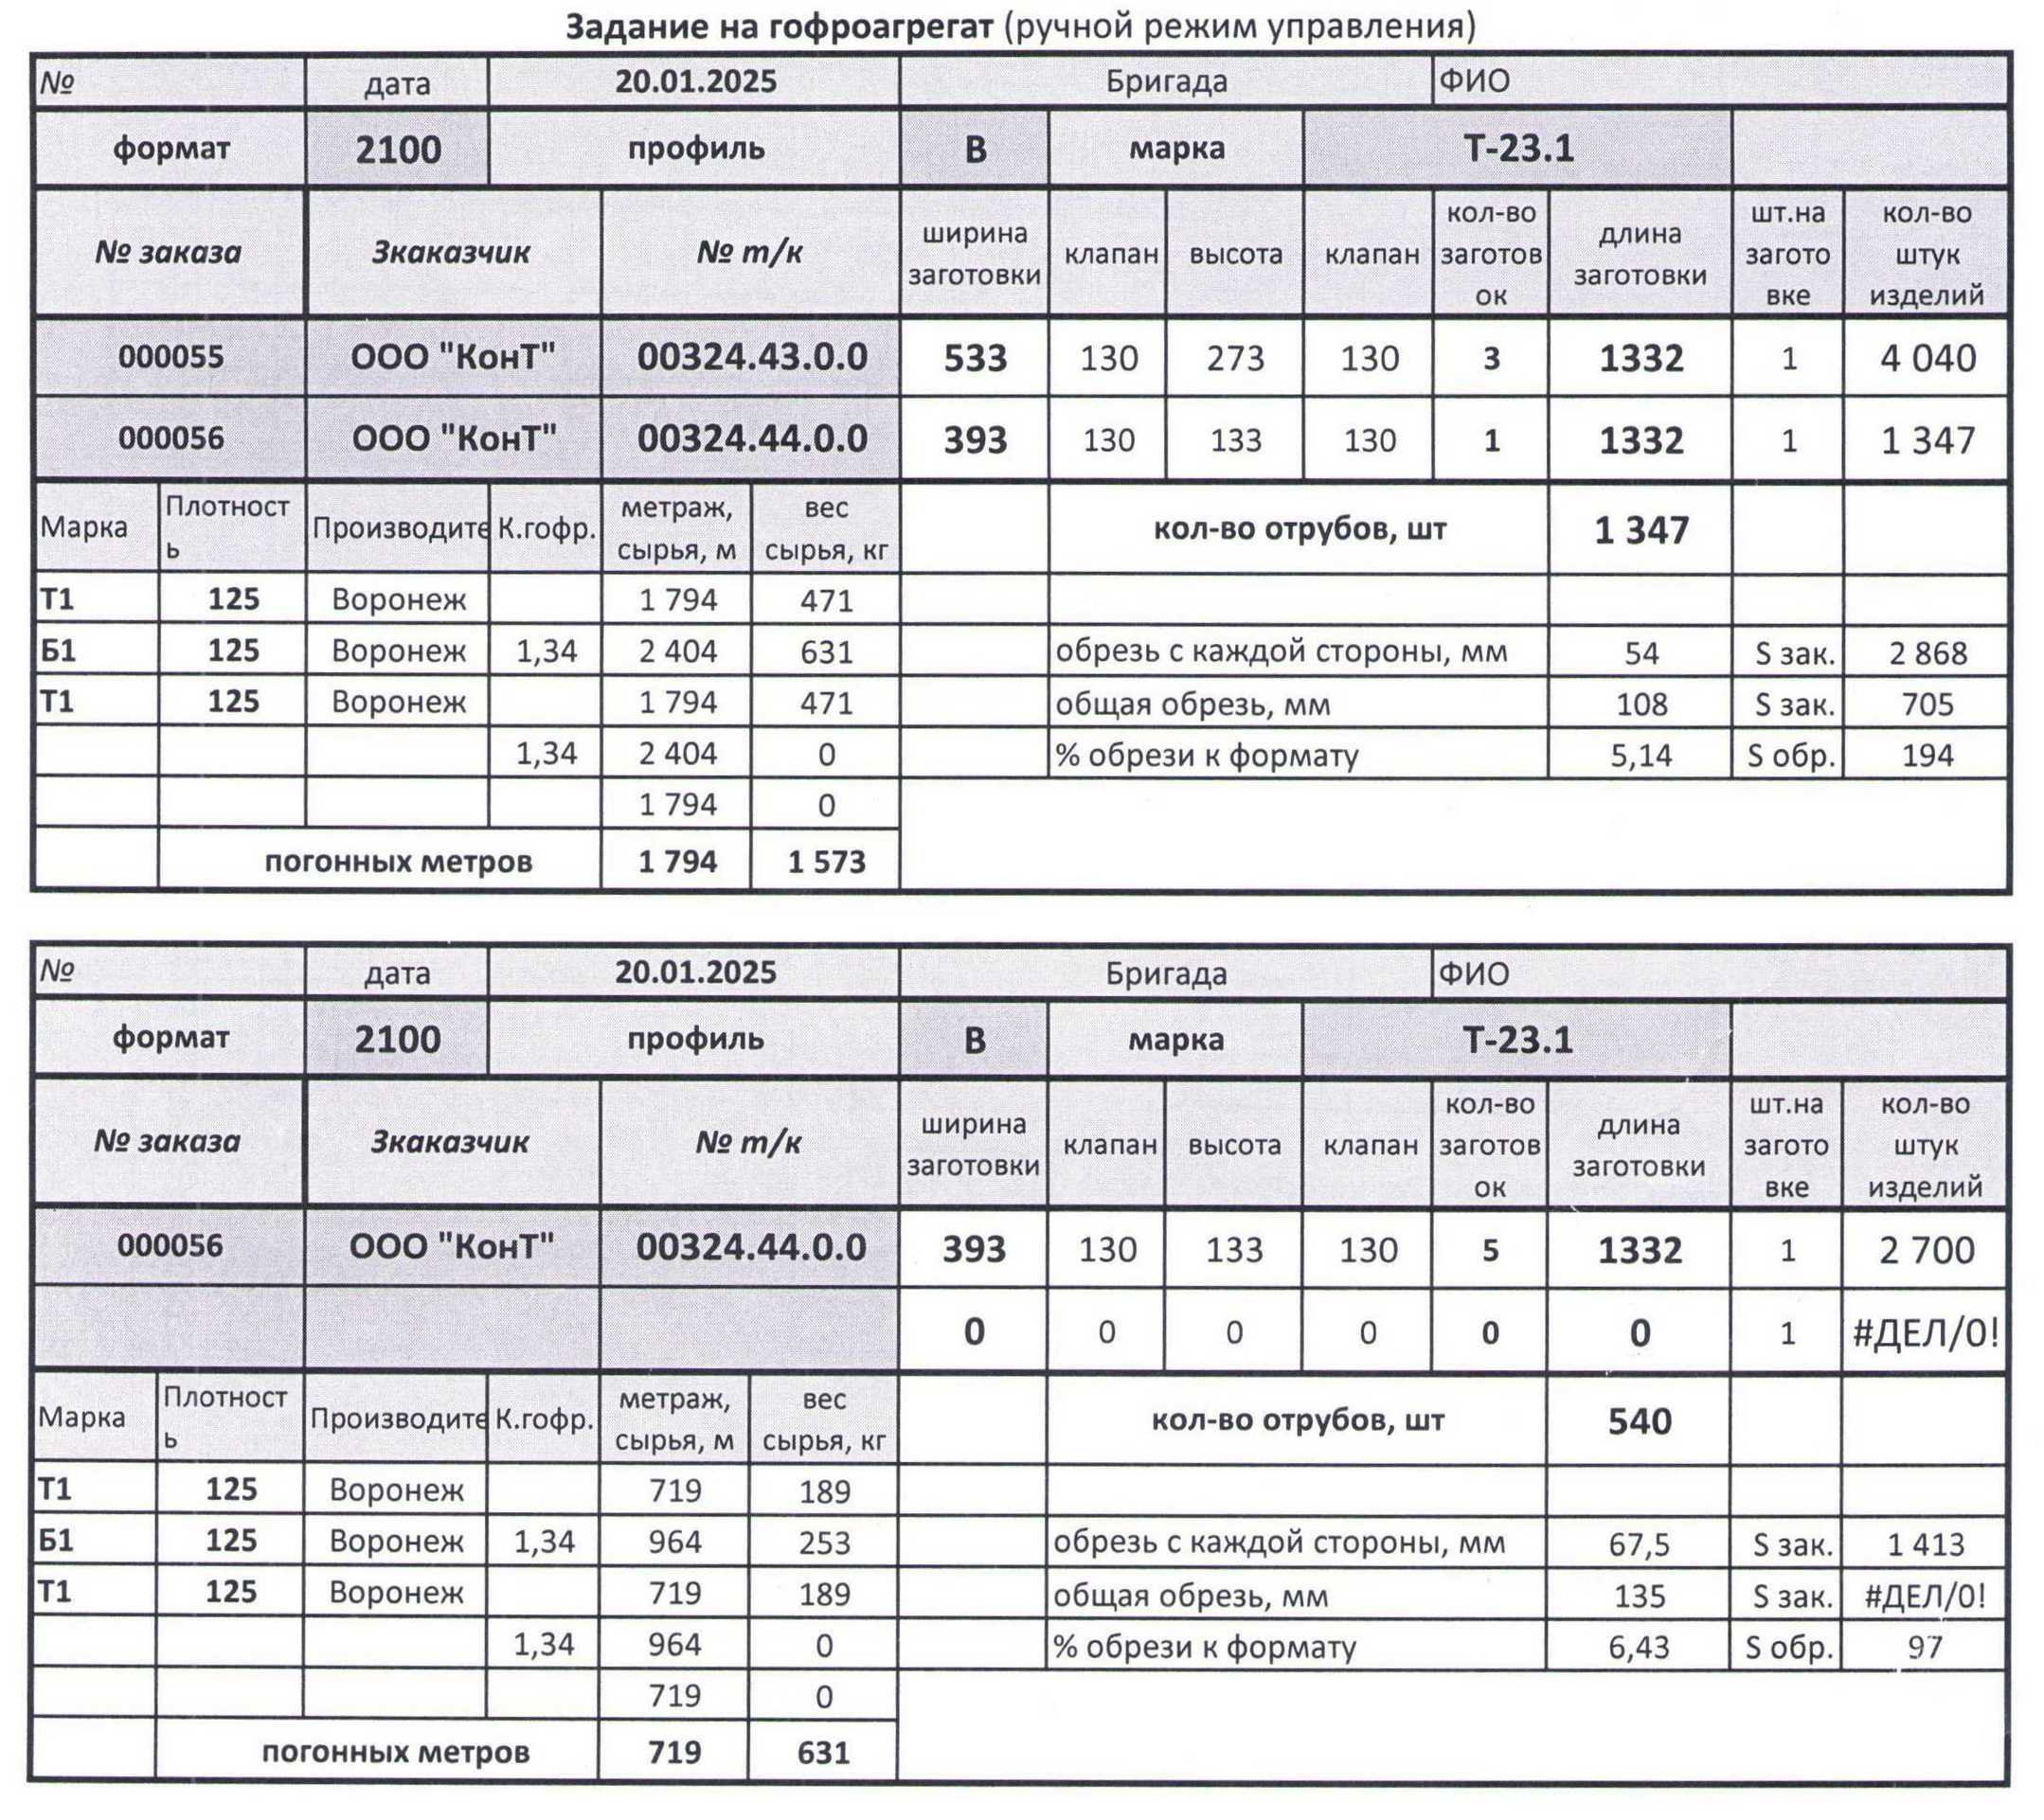
\includegraphics[height=0.94\textheight, width=\textwidth, keepaspectratio]{Pics/f8b.jpg}
\end{center}
\caption{Задание на ГА. Часть 1}
\label{pic:f8b}
\end{figure}

\begin{figure}
\begin{center}
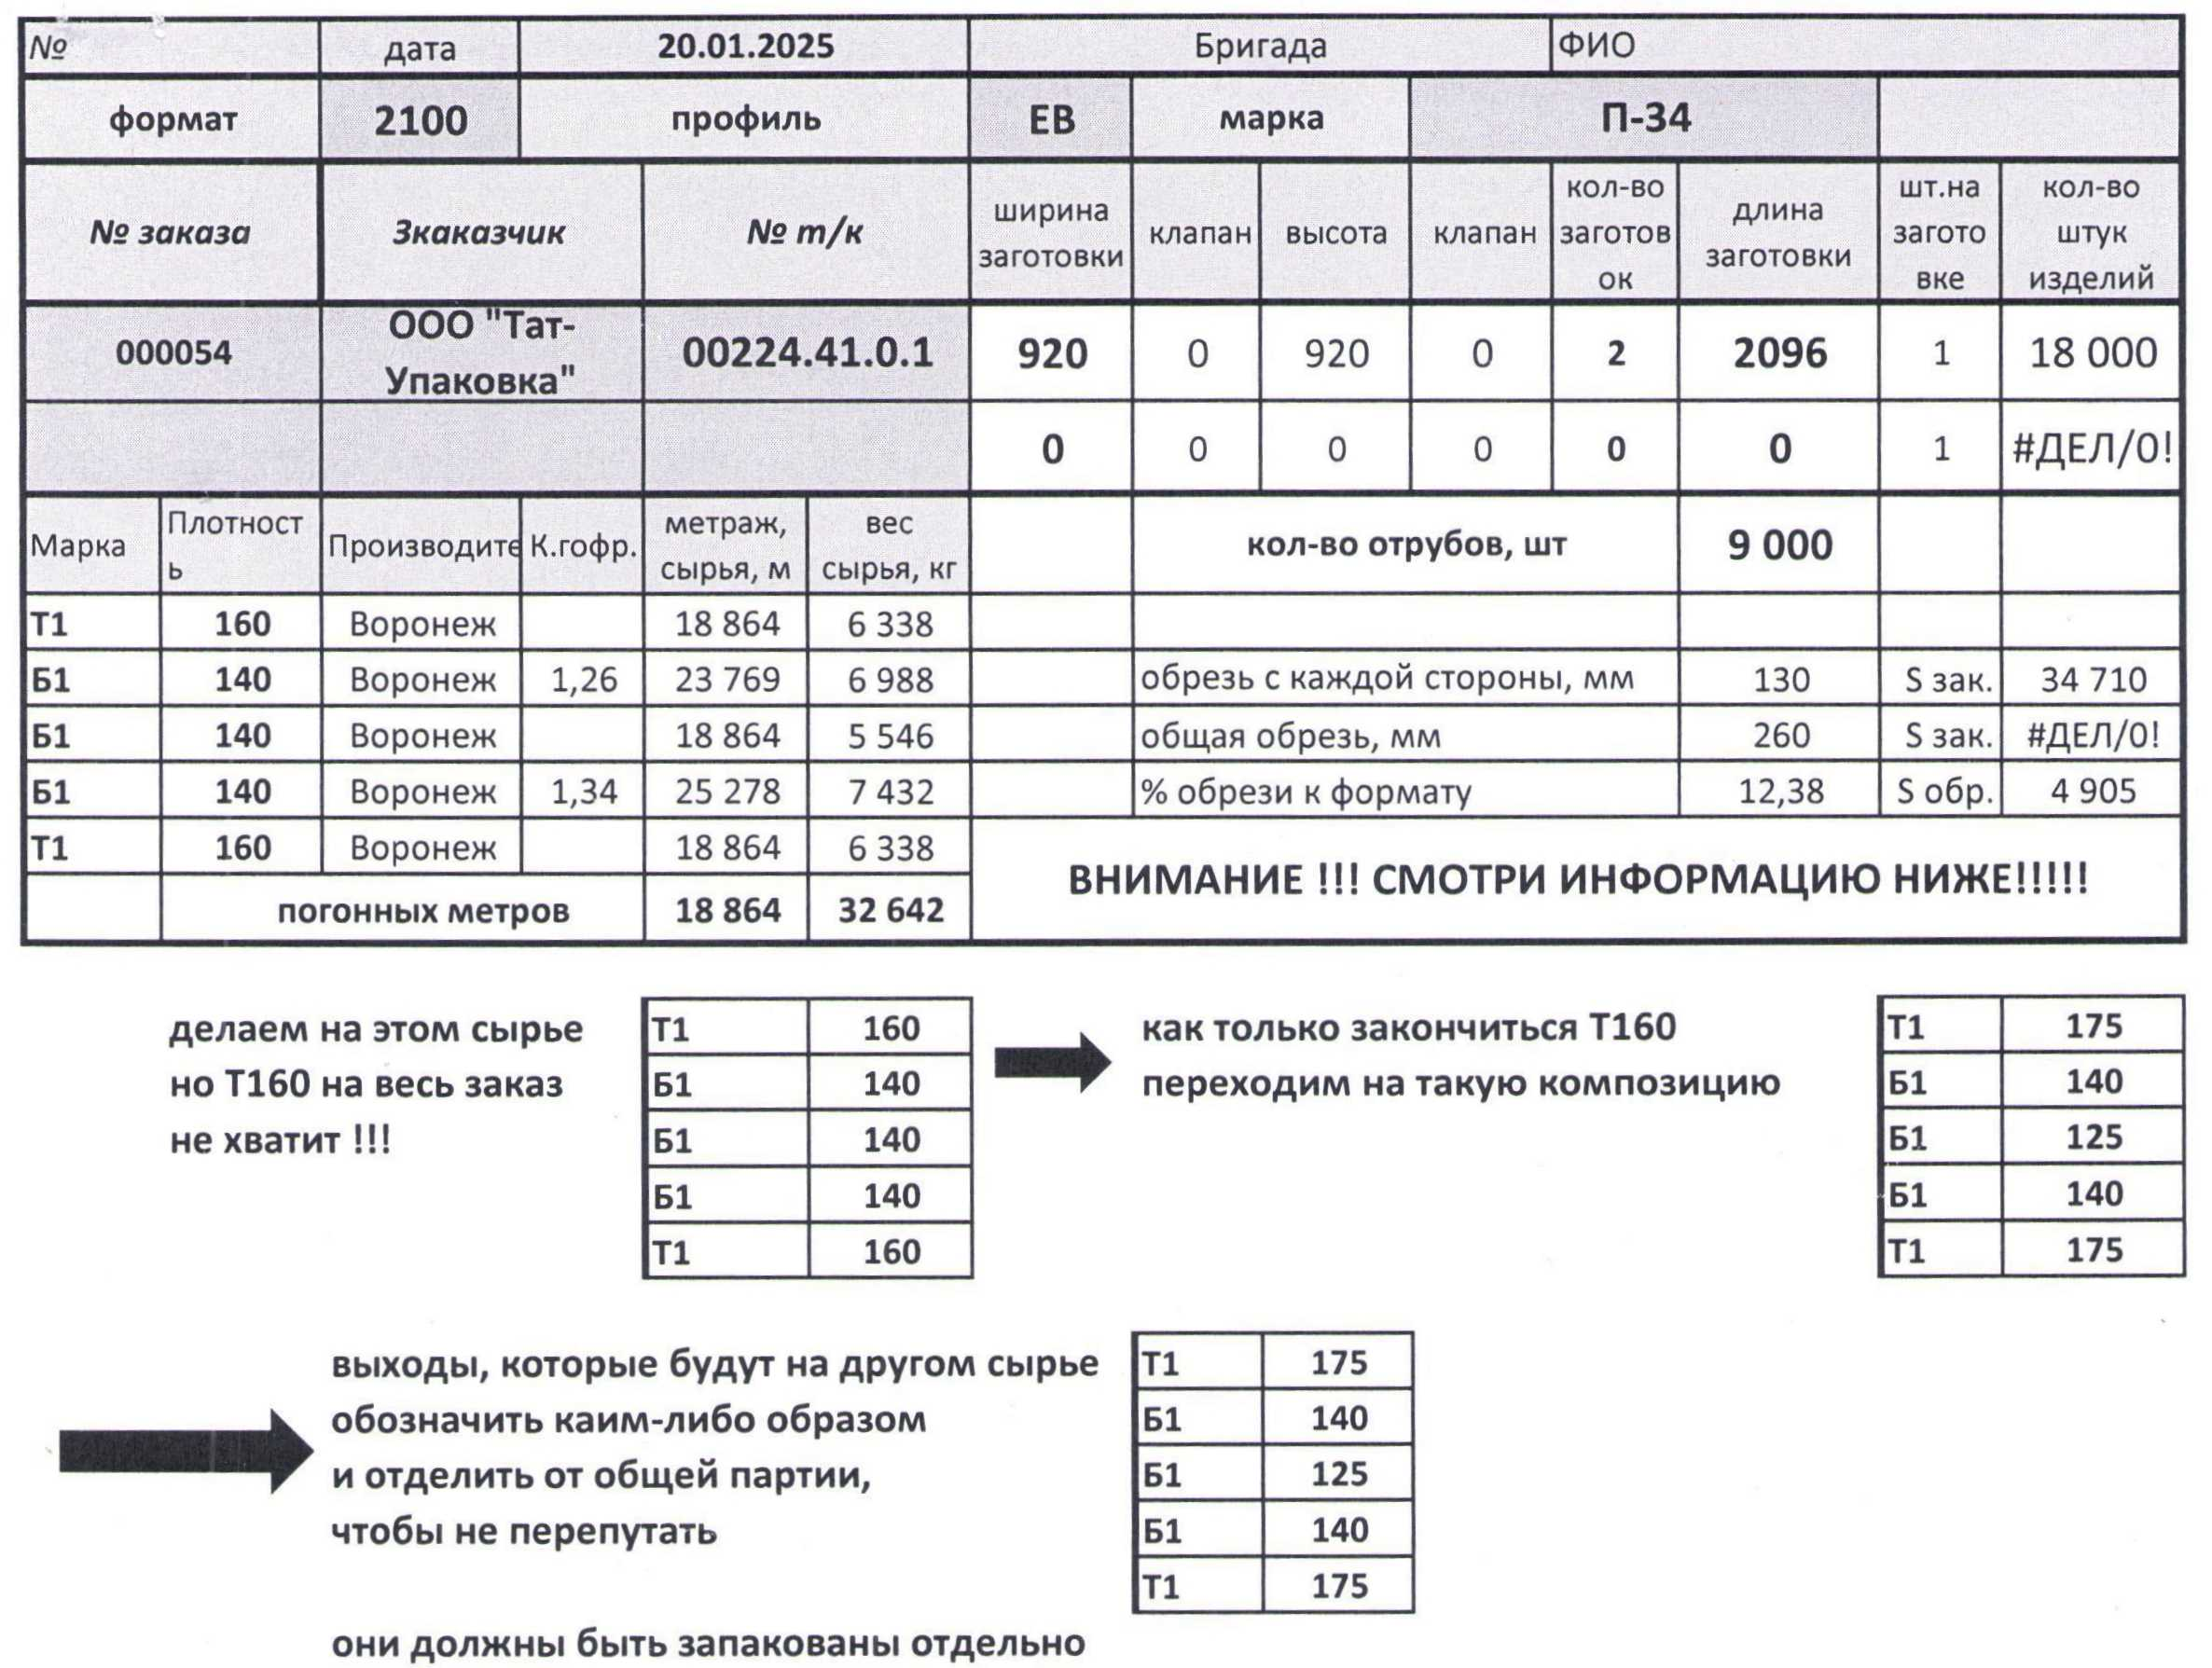
\includegraphics[height=0.94\textheight, width=\textwidth, keepaspectratio]{Pics/f8a.jpg}
\end{center}
\caption{Задание на ГА. Часть 2}
\label{pic:f8a}
\end{figure}

\begin{figure}
\begin{center}
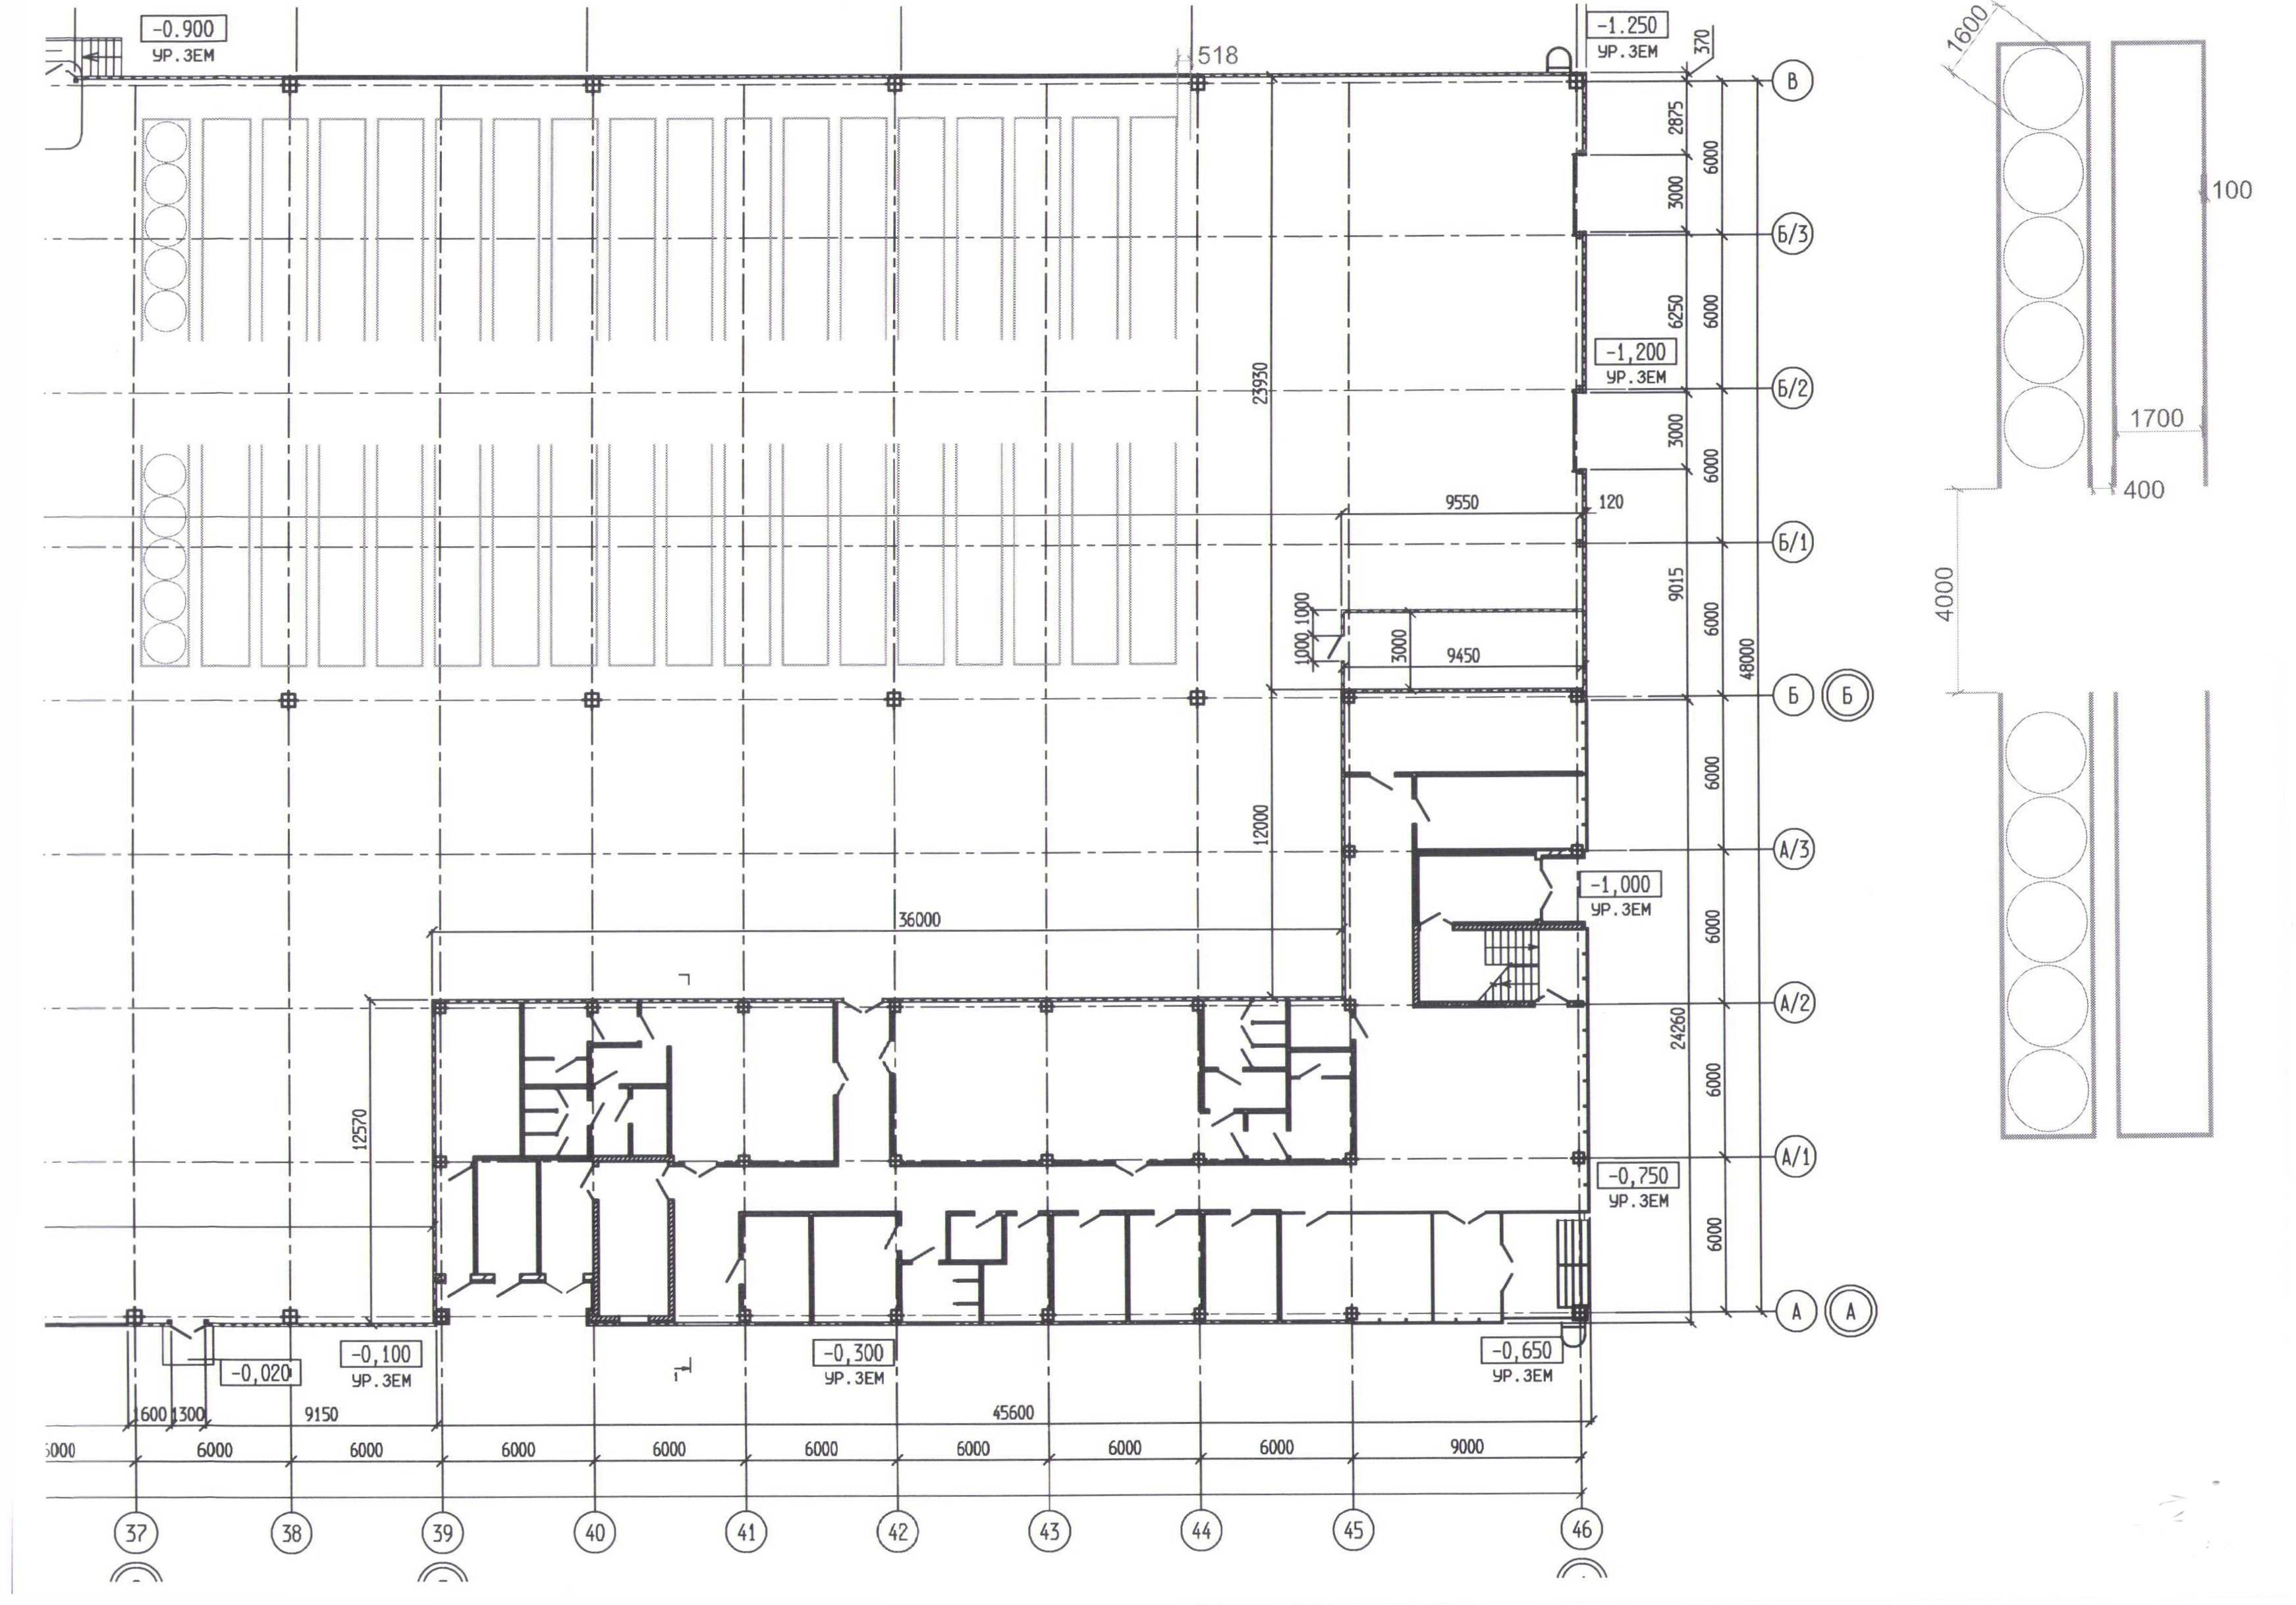
\includegraphics[height=0.94\textheight, width=\textwidth, angle=90, keepaspectratio]{Pics/f4.jpg}
\end{center}
\caption{Склад сырья. Разметка предусматривающая ячеистое хранение продукции}
\label{pic:f4}
\end{figure}

\begin{figure}
\begin{center}
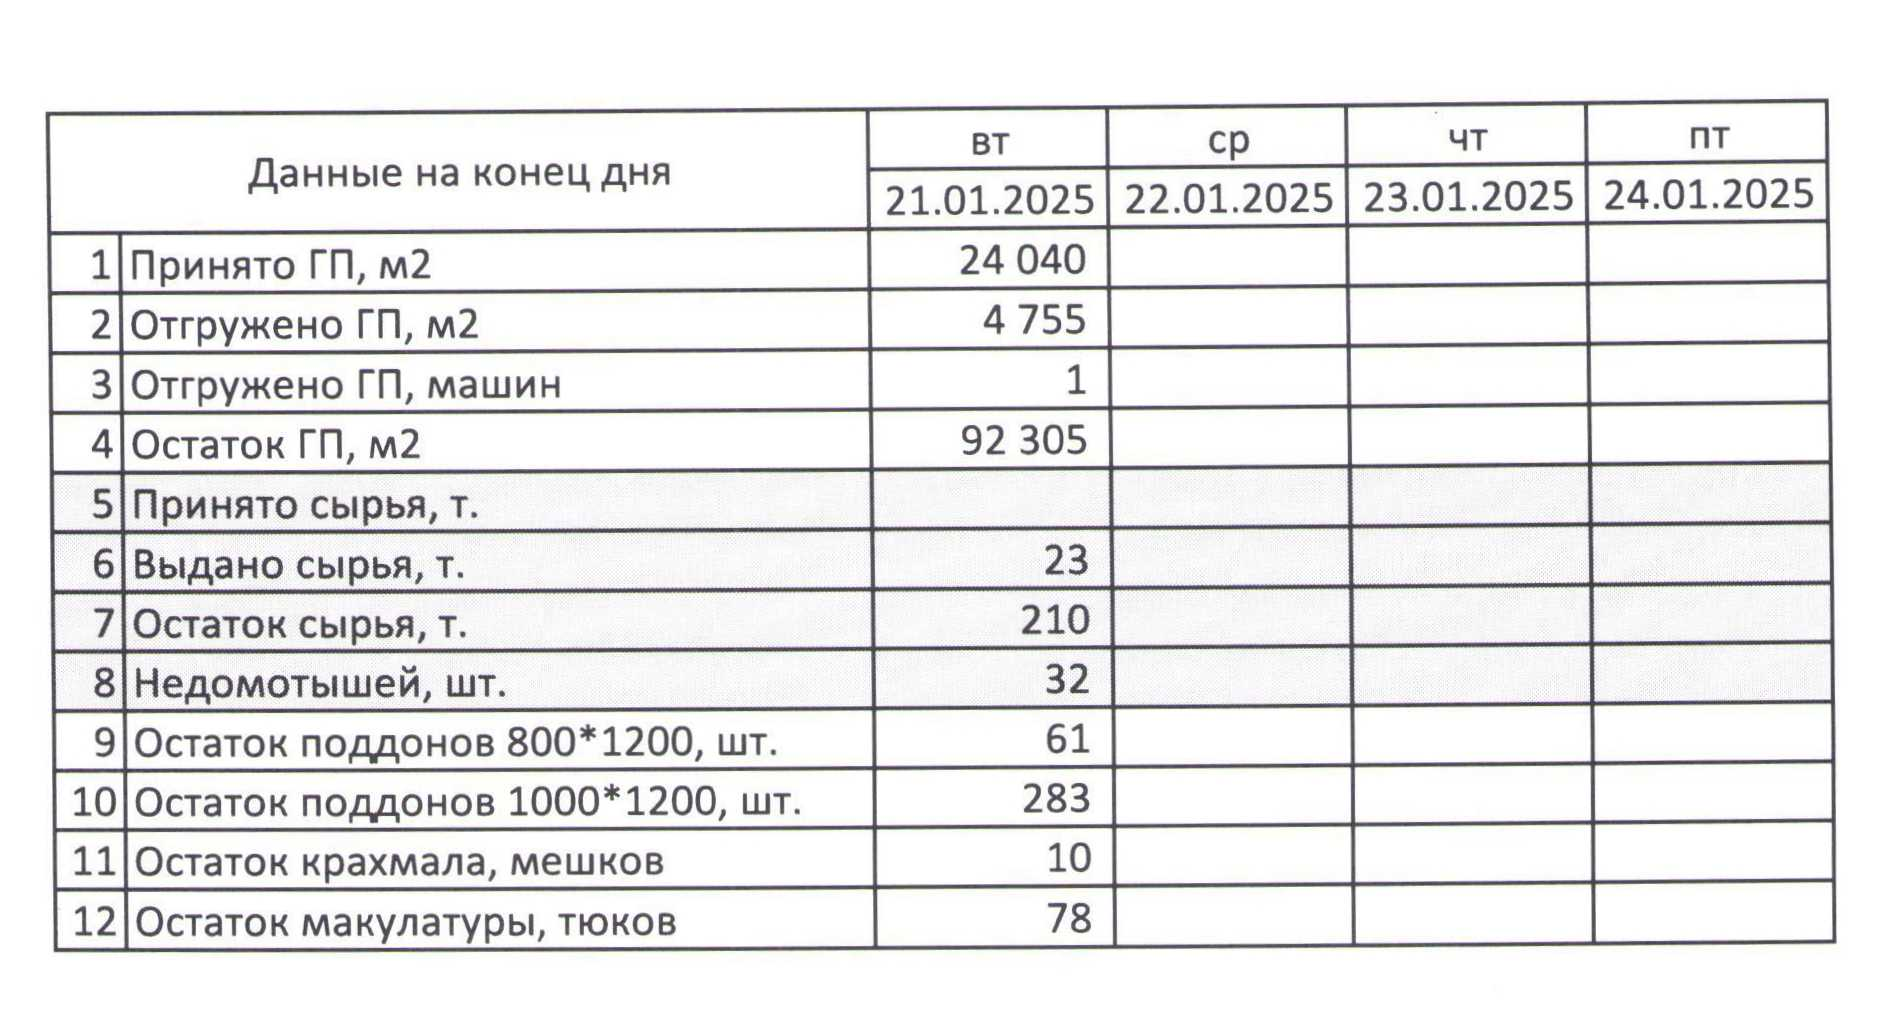
\includegraphics[height=0.94\textheight, width=\textwidth, keepaspectratio]{Pics/f2.jpg}
\end{center}
\caption{Остатки ТМЦ}
\label{pic:f2}
\end{figure}

\begin{figure}
\begin{center}
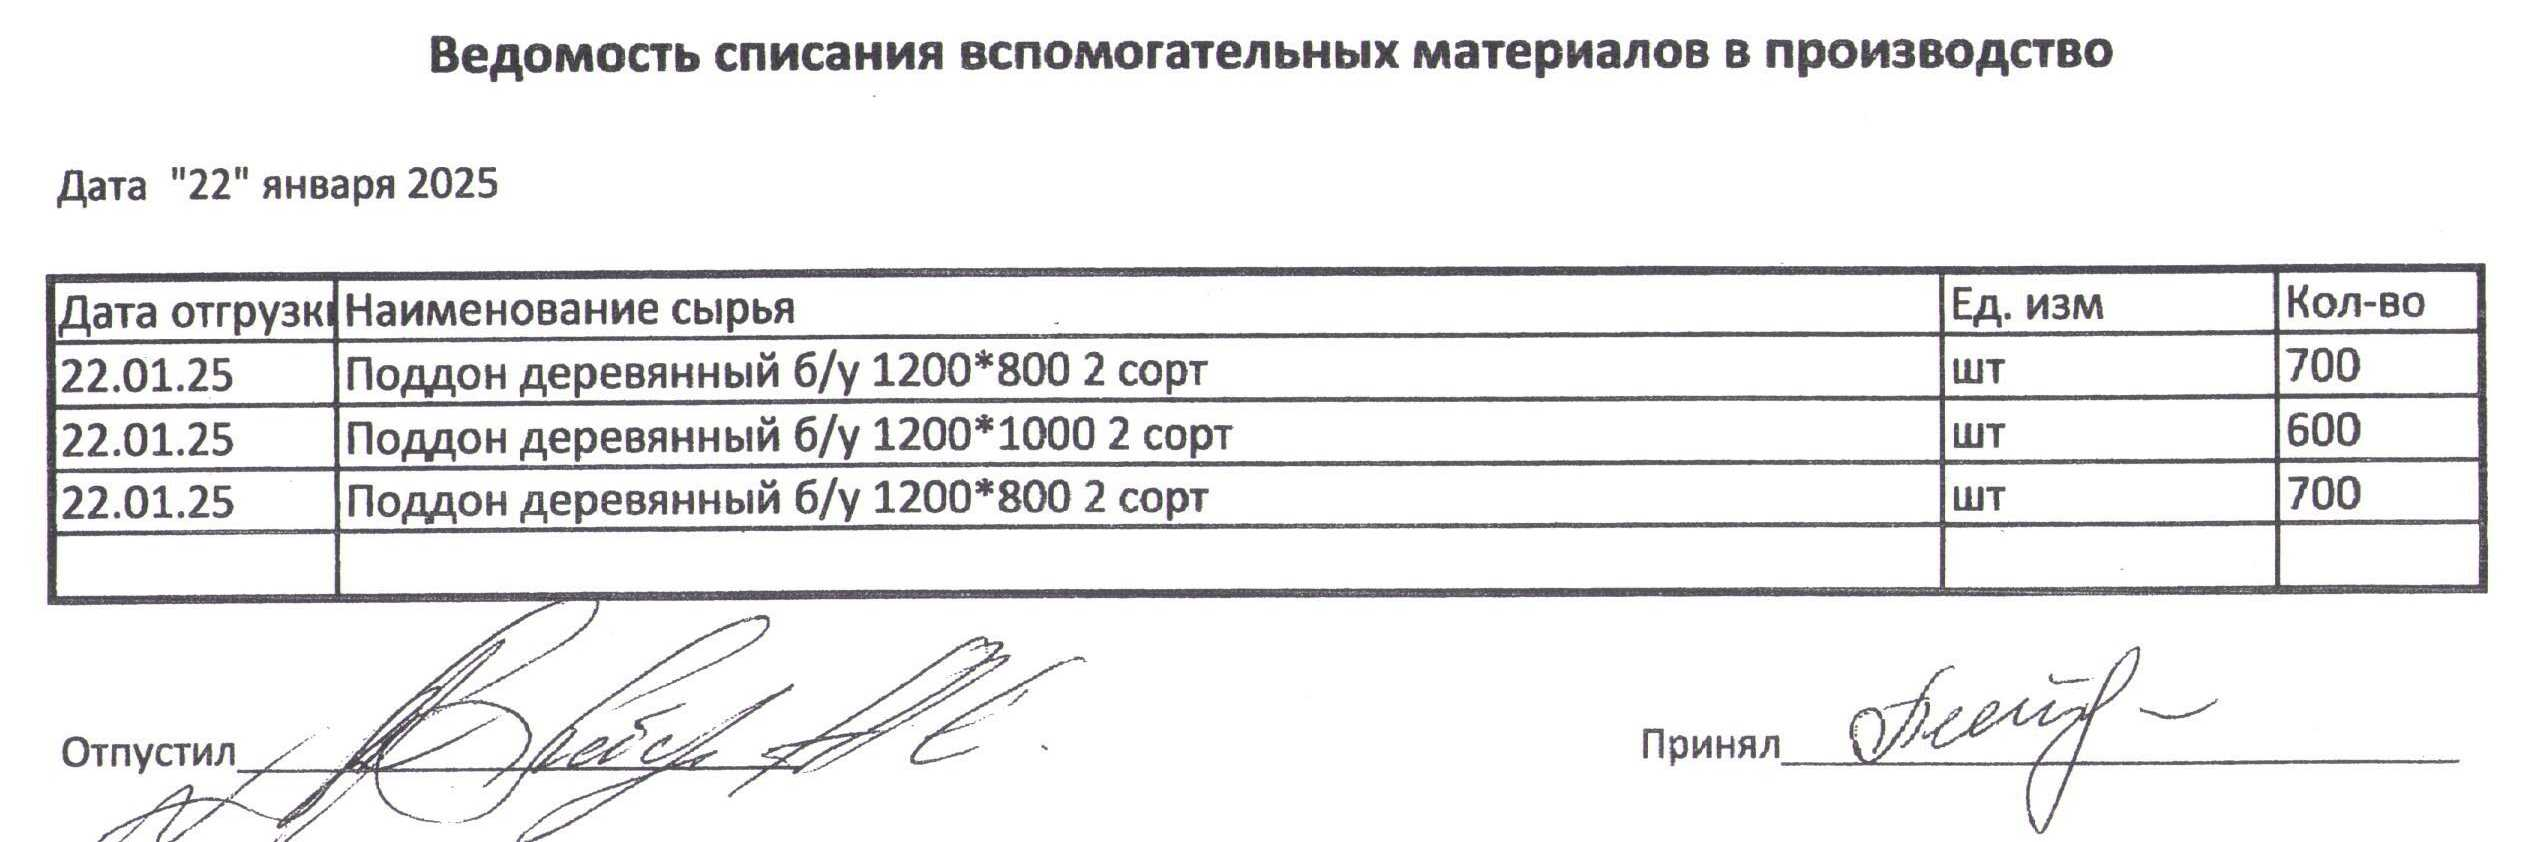
\includegraphics[height=0.94\textheight, width=\textwidth, keepaspectratio]{Pics/f27.jpg}
\end{center}
\caption{Ведомость списания вспомогательных материалов в производство}
\label{pic:f27}
\end{figure}

\clearpage
\ifx \notincludehead\undefined
\normalsize
\end{document}
\fi
% \newpage
%
\subsection{Инвентаризация материалов}
%\label{bp:MatOutput}

На момент обследования инвентаризация не проводилась.

% \clearpage
\ifx \notincludehead\undefined
\normalsize
\end{document}
\fi
% \newpage
\subsection{Управление качеством}
\label{bp:quality}
%\subsection{Управление качеством}

На предприятии создана лаборатория.  Закуплено оборудование. На момент проведения аудита измерения показателей качества не проводились.
%\textcolor{red}{Тут наверное нужно указать введена ли лаборатория в эксплуатацию или находится на стадии оснащения или подбора персонала?}



\clearpage
\ifx \notincludehead\undefined
\normalsize
\end{document}
\fi
% \newpage
\subsection{Претензии контрагентов}
\label{BP_CLaim} 

Процедуры регистрации претензии контрагентов не выявлено. 
Процесс не определен.


\clearpage
\ifx \notincludehead\undefined
\normalsize
\end{document}
\fi
% \newpage
\subsection{Ремонты и ППР}
\label{bp:maintance}


На предприятии создана служба ремонта. 

При поломке оборудования бригадир информирует мастера смены. Мастер смены вызывает необходимого специалиста. Простои фиксирует мастер смены у себя в рапорте. 

Ведется таблица MS EXCEL по поломкам и неисправностям. Машинисты вносят в нее замечания. Служба ремонта вписывает комментарии и сроки устранения (рис. \ref{pic:f28}).





% \newpage
\subsection{Управление закупками}
% %\todo{ÏÈÑÀÒÜ}

 Менеджер по закупкам смотрит остатки ТМЦ в MS EXCEL (рис. \ref{pic:f2}) и, при возникновении необходимости, заказывает необходимые материалы.
% %
% \clearpage
% \ifx \notincludehead\undefined
\normalsize
\end{document}
\fi



% \newpage
\subsection{Управление персоналом}
%\todo{ÏÈÑÀÒÜ}
%
Для автоматизации функций управления персоналом используется программный продукт 1С:ЗУП.

% \newpage
\subsection{Расчет заработной платы}
%\todo{ÏÈÑÀÒÜ}

% Бригадир ведет табели учета рабочего времени (рис. \ref{pic:f44}).


Для расчета ЗП и автоматизации функций управления персоналом используется программный продукт 1С:ЗУП.



% \newpage
\subsection{Ведение бухгалтерского учета}
%\todo{ÏÈÑÀÒÜ}
% %
Для первичного управленческого учета внедряется система «1С:Управление нашей фирмой».

Для ведения бухгалтерского и налогового учета используется система 1С:Бухгалтерия 8.

% \newpage
\subsection{Расчет фактической себестоимости продукции}
%\todo{ÏÈÑÀÒÜ}
% %
Фактическая себестоимость рассчитывается главным бухгалтером котловым методом на весь выпуск продукции в системе 1С:Бухгалтерия 8. 

Учет незавершенного производства на момент аудита не ведется.



%\ifx \notincludehead\undefined
\normalsize
\end{document}
\fi % Описание процессов

\newpage

\chapter{Описание архитектуры информационных систем}




\section{Описание нормативно-справочной информации (НСИ)}

\subsubsection{Справочник <<Номенклатура>>}

Справочник <<Номенклатура>> ведется в системе 1С:Бухгалтерия.
Планируется заполнять справочник в системе 1С:УНФ.

% Справочник совпадает по готовой продукции только в системе 1С: 7.7 ''Бухгалтерия'' и 1С: 7.7 ''Производство+Бухгалтерия+Услуги'', куда он выгружается автоматически через файл MS Excel из системы 1С: 7.7 ''Бухгалтерия''.

% Во всех системах позиции справочника создается вручную. НСИ не согласованы.

Справочник содержит информацию по:
\begin{itemize}
\item основным материалам %(картон, бумага плоских слоев);
\item вспомогательным материалам (клей, материалы для упаковки и т.д.);
\item услугам;
\item готовой продукции.
\end{itemize}

\subsubsection{Справочник <<Контрагенты>>}

Справочник <<Контрагенты>> ведется в системе 1С:Бухгалтерия.
Планируется заполнять справочник в системе 1С:УНФ.

% В каждой базе ведется свой справочник. НСИ не согласованы.
Справочник содержит информацию по:

\begin{itemize}
\item заказчикам продукции;
\item поставщикам материалов;
\item другим организациям и физическим лицам.
\end{itemize}

\subsection{Технологические карты (Спецификации)}

Вся технологическая информация по изготавливаемым изделиям содержится в электронном виде в формате MS EXCEL.  Файлы находятся в сетевом доступе в разных местах хранения.

Единого места хранения не предусмотрено.
%Форма технологической карты представлена на рис. \ref{pic:TK_1} --- \ref{pic:TK_2}.

%\begin{figure}
%\begin{center}
%\ifnum\pdfoutput=0
%%  \includegraphics[40,0][366,292]{Pics/TK0001.jpg}
%\else 
%%  \includegraphics[height=0.94\textheight, keepaspectratio]{Pics/TK0001.jpg}
%\fi
%\end{center}
%  \caption{Пример спецификации по изготавливаемым изделиям}
%  \label{pic:tk}
%\end{figure}
%\clearpage

Основные параметры по технологическим картам
\begin{enumerate}
\item Носитель --- электронный файл и бумажный вариант;
\item Кодирование ---  неформализуемая система кодификации;
\item Поддержка --- дизайнер, конструктор;
%\item Виды нормируемых ресурсов --- только сырье (картон, бумага для гофрирования);
\item Полнота спецификации относительно переменных затрат --- в спецификации содержатся только марка картона и размеры изделия. Нормировано потребление сырья для марок картона.
\item Вариативность и изменение ТК во времени --- ТК изменяется каждый раз при появлении нового заказа.
\item Несколько ТК на номенклатуру --- нет.
\end{enumerate}



\section{Используемые программные продукты}

\subsection{Программы для организации производства}

Для выполнения следующих функций используются таблицы MS EXCEL:
\begin{enumerate}
\item Месячное планирование продаж;
\item Месячное планирование отгрузки;
\item Формирование портфеля заказов;
\item Суточное планирование производства;
\item Подготовка производства (разработка спецификации изделия);
\item Расчет нормативно-плановой себестоимости продукции;
%\item Расчет нормативно-фактической себестоимости продукции;
\item Суточное планирование работы гофроагрегата;
\item Суточное планирование работы перерабатывающих линий;
\item Складской учет материалов и готовой продукции;
%\item Учет претензий контрагентов;
\item Учет выработки на линиях переработки.
% \item Контроль качества.
%\item Производственный учет выпуска готовой продукции.
\end{enumerate}

%Программная система ПОЯС.
%\begin{enumerate}
%\item Планирование раскроев на гофроагрегат в цехе №4.
%\end{enumerate}

Программа Corel Draw.
\begin{enumerate}
\item Разработка дизайна печати технологических карт.


\end{enumerate}

%Программа ArtiosCAD.
%\begin{enumerate}
%\item Разработка раскроев технологических карт сложной высечки.
%\end{enumerate}

% Программа AutoCAD.
% \begin{enumerate}
% \item Разработка штампов технологических карт сложной высечки.
% \end{enumerate}

\subsection{Учетные системы}

\subsubsection{1С:Бухгалтерия 8.3}


Для выполнения учетных функций производства применяется учетная система на
базе 1С:Бухгалтерия. В учетной системе выполняются следующие функции:

% В систему внесены изменения в виде расширений конфигурации.

\begin{enumerate}
\item Бухгалтерский учет материалов;
\begin{enumerate}
\item Поступление ТМЦ;
\item Перемещение ТМЦ;
\item Списание ТМЦ в производство;
\end{enumerate}
%\item Складской учет полуфабрикатов (переделов);
%\begin{enumerate}
%\item Поступление готовой продукции;
%%\item Списание ТМЦ в производство;
%\item Перемещение ТМЦ;
%\end{enumerate}
\item Складской учет готовой продукции;
\begin{enumerate}
\item Оприходование готовой продукции;
\item Отгрузка готовой продукции;
\end{enumerate}
\item Расчет фактической себестоимости продукции;
\item Управление денежными средствами;
% \item Учет основных средств;
\item Управление продажами;
\item Расчеты с поставщиками, подрядчиками и прочими организациями.
% \item Кадровый учет персонала;
% \item Начисление заработной платы работникам;
%\item Начисление налогов с фонда оплаты труда.
% \item Модуль ''Управление взаимоотношениями с клиентами'' (CRM).
%  \item Производственный учет:
%  \begin{enumerate}
% \item Заявки покупателей;
% \item Заявки на отгрузку;
% \item Раскрои на гофроагрегат;
% \item Заказы на поставку заготовок;
% \item Сменный рапорт на линию;

% \item Кадровый учет персонала;
% \item Начисление заработной платы работникам;
% \item Начисление налогов с фонда оплаты труда.
% \end{enumerate}
\end{enumerate}
%

Автоматизированы следующие рабочие места:
\begin{enumerate}
\item Бухгалтерия;
% \item Отдел учета.
% \item Отдел продаж;
%\item Инженер по подготовке производства;
%\item Инженер по организации управления производством;
%\item Машинист гофроагрегата;
% \item Машинист технологической линии (Ishikawa и Минилайн LMC);
%\item Бухгалтер производства.
% \item Склад сырья;
% \item БППП;
% \item Склад готовой продукции;
%\item Логист.
\end{enumerate}


% \subsubsection{1С: Предприятие 8.3 ''Бухгалтерия предприятия''}

% Бухгалтерский учет ведется удаленно на аутсорсинге в системе 1С: Предприятие 8.3 ''Бухгалтерия предприятия''.
% Выполняются стандартные функции по ведению бухгалтерского учета.

% \begin{enumerate}
% % \item Объемное планирование производства;
% \item Управление продажами;
% \item Управление денежными средствами;
% \item Расчеты с поставщиками, подрядчиками и прочими организациями;
% \item Бухгалтерский учет;
% \item Налоговый учет.
% \end{enumerate}

% Автоматизированы следующие рабочие места:
% \begin{enumerate}
% \item Отдел учета;
% \item Отдел продаж и закупок.
% \end{enumerate}




%
\subsubsection{1С:Зарплата и управление персоналом 8}
В учетной системе выполняются следующие функции.
\begin{enumerate}
\item Кадровый учет персонала;
\item Начисление заработной платы работникам;
\item Начисление налогов с фонда оплаты труда.
\end{enumerate}

Автоматизированы следующие рабочие места:
\begin{enumerate}
\item Бухгалтерия.
\end{enumerate}


\ifx \notincludehead\undefined
\normalsize
\end{document}
\fi  % Архитектура и оборудование
\newpage

\chapter{Описание технологической архитектуры}

\section{Компьютерное обеспечение и сеть}

На предприятии организована локальная сеть . 
% Удаленные рабочие места подключаются через удаленное соединение.

В производственном помещении организована безпроводная Wi-fi сеть.




\textbf{Сервера}

% Внутреннего сервера нет. 
% Используется виртуальный сервер в облаке МТС.

% Файловое хранилище также в облаке МТС.

Сервер с параметрами. 
% Среда виртуализации Proxmox Virtual Environment.
\begin{enumerate}
\item Intel Xeon Silver 4314; 
\item  256ГБ оперативной памяти;
\item SSD рейд-массив;
\item БД PostgreSQL.
\end{enumerate}

%\todo[]{Получить данные по серверу}
% \

% %
%В сети выделено ????  рабочих места (компьютеров) включая удаленные.

% \textbf{Площадка 1}
% \begin{enumerate}
%     \item Менеджеры 7 рабочих станций;
%     \item Учет 3 рабочие станции;
%     \item  Руководители 2 рабочие станции;
%     \item Фин отдел 2 рабочие станции;
%     \item Дизайнер 1 рабочая станция.
% \end{enumerate}

% \textbf{Площадка 2}
% \begin{enumerate}
%     \item Менеджеры 7 рабочих станций;
%     \item Учет 3 рабочие станции;
%     \item  Руководители 2 рабочие станции;
%     \item Фин отдел 2 рабочие станции;
%     \item Дизайнер 1 рабочая станция.
% \end{enumerate}

% \textbf{Площадка 3}
% \begin{enumerate}
%     \item Менеджеры 7 рабочих станций;
%     \item Учет 3 рабочие станции;
%     \item  Руководители 2 рабочие станции;
%     \item Фин отдел 2 рабочие станции;
%     \item Дизайнер 1 рабочая станция.
% \end{enumerate}


 \section{Список технологического оборудования}

\subsection{Гофроагрегат}

Гофроагрегат HSIEH HSU.

%\scriptsize
\begin{longtable}{|p{10cm}|p{5cm}|}
    \hline
	\textbf{Характеристика} & \textbf{Значение}
	\endhead
	\hline
	СКОРОСТЬ МАКСИМАЛЬНАЯ       	 &  350 м/мин\\
  	\hline
  	СКОРОСТЬ РАБОЧАЯ                 &  350 м/мин\\
  	\hline
Минимальный формат & 175х500\\
  	\hline
Максимальный формат & 2500х3500\\
  	\hline
  	Максимальное количество рилевок & 12 шт. \\
  	 	\hline
  	Максимальное количество ножей& 7 шт.\\   
  	\hline
Профиль гофра                  	         &В, С, Е, ВС, ЕВ, ЕС \\
    \hline
  \caption{Гофроагрегат}
  \label{tab:corrugator1}
\end{longtable}
\normalsize


% Гофроагрегат: J.S.M

% %\scriptsize
% \begin{longtable}{|p{10cm}|p{5cm}|}
%     \hline
% 	\textbf{Характеристика} & \textbf{Значение}
% 	\endhead
% 	\hline
% 	СКОРОСТЬ МАКСИМАЛЬНАЯ       	 &  250 м2/мин\\
%   	\hline
%   	СКОРОСТЬ РАБОЧАЯ                 &  210 м2/мин\\
%   	\hline
% Минимальный формат & 1800мм\\
%   	\hline
% Максимальный формат & 2200мм\\
%   	\hline
%   	Максимальное количество рилевок & 12 шт.\\
%   	 	\hline
%   	Максимальное количество ножей& 7 шт.\\   	\hline
% Профиль гофры                  	         &В, С \\
%     \hline
%   \caption{Гофроагрегат 2}
%   \label{tab:corrugator1}
% \end{longtable}
% \normalsize

% %%%\begin{longtable}{|p{10cm}|p{5cm}|}
%   %  \hline
% %	\textbf{Характеристика} & \textbf{Значение}
% %	\endhead
% %	\hline
% %	СКОРОСТЬ МАКСИМАЛЬНАЯ       	 &  240 п.м./мин\\
%  %	\hline
%  % 	СКОРОСТЬ РАБОЧАЯ                 &  150 п.м./мин\\   	\hline Минимальный формат & 1050мм\\   
%  % 	\hline
% % Максимальный формат & 1750мм\\
%  %  	\hline
%   % 	Максимальное количество рилевок & 12мм\\
%   % 	\hline
% % Профиль гофры                  	         &В, С, ВС\\
%   %   \hline
%   % \caption{Гофроагрегат}
%   % \label{tab:corrugator}
% % \end{longtable}
%  %\normalsize

% %
% %% Table generated by Excel2LaTeX from sheet 'Лист1'
% %\scriptsize
% %\begin{longtable}{|p{20mm}|p{20mm}|p{27mm}|p{20mm}|p{40mm}|p{20mm}|}
% %\hline
% %\parbox[c][6mm]{20mm}{\raggedright Наименование} & \parbox[c]{20mm}{\raggedrightНазначение} & \parbox[c]{27mm}{\raggedrightПрофиль} & \parbox[c]{20mm}{\raggedright Макс. Производительность в мин. Циклов} & \parbox[c]{40mm}{\raggedrightФормат } & \parbox[c]{20mm}{\raggedrightМесто расположения} \\
% %\hline
% %\parbox[c][19mm]{39mm}{JETS 300} & \parbox{27mm}{Гофроагрегат} & \parbox{27mm}{B,C,E,BC,BE,CE} & \parbox{75mm}{250-300} & \parbox{57mm}{1260,1400,2000,2100,2450,2500.} & \parbox{57mm}{Цех № 1} \\
% %\hline
% %\caption{Гофроагрегат 1}\label{tab:ga2}
% %\end{longtable}  
% %\normalsize
% %
% %
% %\newpage
% %Гофроагрегат 2
% %
% %% Table generated by Excel2LaTeX from sheet 'Лист1'
% %\scriptsize
% %\begin{longtable}{|p{20mm}|p{20mm}|p{27mm}|p{20mm}|p{40mm}|p{20mm}|}
% %\hline
% %\parbox[c][6mm]{20mm}{\raggedright Наименование} & \parbox[c]{20mm}{\raggedrightНазначение} & \parbox[c]{27mm}{\raggedrightПрофиль} & \parbox[c]{20mm}{\raggedright Макс. Производительность в мин. Циклов} & \parbox[c]{40mm}{\raggedrightФормат } & \parbox[c]{20mm}{\raggedrightМесто расположения} \\
% %\hline
% %\parbox[c][19mm]{39mm}{ХХХХ} & \parbox{27mm}{Гофроагрегат} & \parbox{27mm}{B,C,E,BC,BE,CE} & \parbox{75mm}{250-300} & \parbox{57mm}{1260,1400,2000,2100,2450,2500.} & \parbox{57mm}{Компания 'Гофромастер'} \\
% %\hline
% %\caption{Гофроагрегат 1}\label{tab:ga2}
% %\end{longtable}  
% %\normalsize
\subsection{Технологические линии}

\subsubsection{Перерабатывающая линия изготовления ящиков SHINKO 618}
\begin{longtable}{|p{10cm}|p{5cm}|}
    \hline
	\textbf{Характеристика} & \textbf{Значение}
	\endhead
	\hline
скорость максимальная       	 & 24000 шт/ч\\
  %	\hline 
%скорость рабочая                         	& 250 м/м\\
  	\hline 
размер заготовки минимальный  	& 200 x 500   \\	
  	\hline 
  	размер заготовки максимальный   & 600 x 1800  \\
  	\hline 
количество секций:    	& секция подачи\\
& 3 покрасочных секции \\
& 1 слоттерная секция\\
& 1 ротационная секция.\\
& 1 фальцевально-склеивающая секция \\
%& накопительный бункер\\
%& стреппинг-машина MOSKA\\
\hline 
  \caption{SHINKO 618}\label{tab:line1}
\end{longtable}


\subsubsection{Перерабатывающая линия изготовления ящиков SHINKO 924}
\begin{longtable}{|p{10cm}|p{5cm}|}
    \hline
	\textbf{Характеристика} & \textbf{Значение}
	\endhead
\hline
скорость максимальная       	 & 21000 шт/ч\\
  %%скорость рабочая                         	& 250 м/м\\
  	\hline 
размер заготовки минимальный  	& 280 x 755  \\	
  	\hline 
  	размер заготовки максимальный   & 880 x 2400  \\
  	\hline 
количество секций:    	& секция подачи\\
& 4 покрасочных секции \\
& 1 слоттерная секция\\
& 1 ротационная секция\\
& 1 фальцевально-склеивающая секция\\
%& накопительный бункер\\
%& стреппинг-машина MOSKA\\
\hline 
  \caption{SHINKO 924}\label{tab:line2}
\end{longtable}



\subsubsection{Перерабатывающая линия SHINKO   1628 L}
\begin{longtable}{|p{10cm}|p{5cm}|}
    \hline
	\textbf{Характеристика} & \textbf{Значение}
	\endhead
	\hline
 скорость максимальная       	 & 12000 шт/ч\\
%  	\hline 
%скорость рабочая                         	& 250 м/м\\
  	\hline 
размер заготовки минимальный  	& 420 x 710   \\	
  	\hline 
  	размер заготовки максимальный   & 1570 x 2800  \\
  	\hline 
количество секций:    	& секция подачи\\
& 4 покрасочных секции \\
%& 1 слоттерная секция\\
& 1 ротационная секция.\\
% & секция сбора в стопы. \\
%& накопительный бункер\\
%& стреппинг-машина MOSKA\\
\hline 
  \caption{SHINKO   1628 L}\label{tab:line3}
\end{longtable}

\subsubsection{Перерабатывающая линия SHINKO   1628 R}
\begin{longtable}{|p{10cm}|p{5cm}|}
    \hline
	\textbf{Характеристика} & \textbf{Значение}
	\endhead
	\hline
 скорость максимальная       	 & 12000 шт/ч\\
  %	\hline 
%скорость рабочая                         	& 250 м/м\\
  	\hline 
размер заготовки минимальный  	& 420 x 710   \\	
  	\hline 
  	размер заготовки максимальный   & 1570 x 2800  \\
  	\hline 
количество секций:    	& секция подачи\\
& 4 покрасочных секции \\
%& 1 слоттерная секция\\
& 1 ротационная секция.\\
% & секция сбора в стопы. \\
%& накопительный бункер\\
%& стреппинг-машина MOSKA\\
\hline 
  \caption{SHINKO   1628 R}\label{tab:line4}
\end{longtable}


\subsubsection{Перерабатывающая линия ASAHI AP-165 EII}

\begin{longtable}{|p{10cm}|p{5cm}|}
    \hline
	\textbf{Характеристика} & \textbf{Значение}
	\endhead
	\hline
скорость максимальная       	 & 5000  шт./час\\
\hline 
%скорость рабочая                 & 250   м/м\\
 	%\hline 
размер заготовки минимальный  	& 500 x 600       \\	
  	\hline 
  	размер заготовки максимальный   & 1200 x 1650\\
  	\hline 
количество секций:    	& секция подачи\\
& 4 покрасочных секции\\
%& 1 слоттерная секция\\
& 1 секция плоской высечки\\
% & фальцевально-склеивающая секция\\
%& накопительный бункер\\
%& стреппинг-машина MOSKA\\
  	\hline 
 \caption{ASAHI AP-165 EII}\label{tab:line5}
\end{longtable}


% \subsubsection{Резательный станок  Packsize}

% \begin{longtable}{|p{10cm}|p{5cm}|}
%     \hline
% 	\textbf{Характеристика} & \textbf{Значение}
% 	\endhead
% 	\hline
% скорость максимальная       	 & 2    сек./шт.\\
%   	\hline 
% скорость рабочая                 & 10   сек./шт.\\
%   	\hline 
% размер заготовки минимальный  	& 500 мм                \\	
%   	\hline 
%   	размер заготовки максимальный   & 2400 мм\\
%   	\hline 
% \caption{Резательный станок  Packsize} \label{tab:line17}
% \end{longtable}


% \subsubsection{Резательный станок  Packsize}

% \begin{longtable}{|p{10cm}|p{5cm}|}
%     \hline
% 	\textbf{Характеристика} & \textbf{Значение}
% 	\endhead
% 	\hline
% скорость максимальная       	 & 2    сек./шт.\\
%   	\hline 
% скорость рабочая                 & 10   сек./шт.\\
%   	\hline 
% размер заготовки минимальный  	& 500 мм                \\	
%   	\hline 
%   	размер заготовки максимальный   & 2400 мм\\
%   	\hline 
% \caption{Резательный станок  Packsize} \label{tab:line17}
% \end{longtable}


% \subsubsection{Резательный станок  Packsize}

% \begin{longtable}{|p{10cm}|p{5cm}|}
%     \hline
% 	\textbf{Характеристика} & \textbf{Значение}
% 	\endhead
% 	\hline
% скорость максимальная       	 & 2    сек./шт.\\
%   	\hline 
% скорость рабочая                 & 10   сек./шт.\\
%   	\hline 
% размер заготовки минимальный  	& 500 мм                \\	
%   	\hline 
%   	размер заготовки максимальный   & 2400 мм\\
%   	\hline 
% \caption{Резательный станок  Packsize} \label{tab:line17}
% \end{longtable}

%\subsubsection{Фальцевально-склеивающая машина SYKM4215-2400}

%\begin{longtable}{|p{10cm}|p{5cm}|}
%    \hline
%	\textbf{Характеристика} & \textbf{Значение}
%	\endhead
%	\hline
%скорость максимальная       	 & 100  шт./мин\\
%  	\hline 
%скорость рабочая                 & 90   шт./мин\\
%	\hline 
%размер заготовки минимальный  	& 340 x 875       \\	
 % 	\hline 
 % 	размер заготовки максимальный   & 1300 x 2040\\
 % 	\hline 
%количество секций:    	& секция подачи\\
%& 2 покрасочных секции (2 - ракельных)\\
%& 1 слоттерная секция\\
%& 1 ротационная секция\\
%& фальцевально-склеивающая секция\\
%& накопительный бункер\\
%& стреппинг-машина MOSKA\\
  %	\hline 
% \caption{SYKM4215-2400}\label{tab:line8}
%\end{longtable}

% \subsubsection{Перерабатывающая линия изготовления ящиков с двухцветной печатью Альфа}
% \begin{longtable}{|p{10cm}|p{5cm}|}
%     \hline
% 	\textbf{Характеристика} & \textbf{Значение}
% 	\endhead
% 	\hline
% скорость максимальная       	 & 125 шт/мин.\\
%   	\hline 
% скорость рабочая                         	& 100 шт/мин.\\
%   	\hline 
% размер заготовки минимальный  	& 690х320        \\	
%   	\hline 
%   	размер заготовки максимальный   & 2850х1200\\
%   	\hline 
% количество секций:    	& секция подачи\\
% & 2 покрасочных секции \\
% %& 1 слоттерная секция\\
% & 1 ротационная секция.\\
% %& фальцевально-склеивающая секция\\
% %& накопительный бункер\\
% %& стреппинг-машина MOSKA\\
%   	\hline 
%   \label{tab:line1}
% \end{longtable}



\ifx \notincludehead\undefined
\normalsize
\end{document}
\fi  % Словарь терминов и сокращений
\newpage

\chapter{Заключение}

\section{Описание <<узких мест>> производства}



\begin{enumerate}

\item Предприятие новое и бизнес-процессы полностью не сформированы.

\item Все данные переносятся вручную, от заведения заказов, до планирования.

\item 	Не ведётся учет неснижаемого запаса по материалам.
%Списание происходит раз в месяц и при заказе вспомогательных материалов закупщику не на что ориентироваться.

\item 	Не ведется журнал выдачи-приемки оснастки.

\item 	Не ведется пробег по оснастке.

\item  Ремонт оснастки не фиксируется.
 
\item  Не ведется учет заявок оснастки.
 
 \item  Нормы и композиции сырья отсутствуют.
 
 \item  Отсутствует расчет объемов необходимой краски на заказ.
 
 %\item Прием краски осуществляет техник УВФ, а списание в бухгалтерии. Есть вероятность появления ошибки при поступлении.

%\item 	ТК хранятся на УВФ в распечатанном виде. При внесении изменений ТК меняется на новую вручную, в связи с чем существует риск выпуска продукции по старой версии ТК.

%\item  Основная ТК и лист укладки на поддон  

%\item  Отсутствуют номера ТК. Необходимую ТК ищут по названию клиента и размерам. Есть вероятность не найти нужную ТК. 

%\item  На сервере ТК в электронном виде хранятся по раздельности (четырехклапанный короб, сложная высечка, дизайн, упаковка). Отсутствует единое хранилище технологической документации.

\item  Бирки ГП печатает мастер смены. Существует риск ошибиться с номенклатурой и количеством.

\item Сырье списывается на производство целыми рулонами, остатки рулонов не взвешиваются, нет весового учета остатков.

\item Не ведется расход сырья на производстве.

\item На производстве не выявлено четкого учета брака.

\item  Расчет необходимого объема сырья (бумага, картон) бригадир ГА осуществляет в уме.

\item  Бирка ПФ - отсутствует количество на поддоне.

\item  Для складской службы не выделены помещения в местах хранения ТМЦ как по готовой продукции, так по сырью (бумага и картон), вспомогательным материалам.

%\item  Отсутствие планирования линий переработки.  На смену могут быть заказы на оду, две линии.  Остальные линии могут простаивать.

%\item  Служба ОТК не участвует в приемки сырья. Измерения проводят по факту дефектов на ГА.


%\item 	В ярлыке на ГП мастер меняет количество на поддоне в зависимости от транспорта под загрузку. Отсутствует четкий транспортный пакет.

%\item 	При физической сверке заготовки в цеху выявляются ошибки, допущенные при списании или оприходовании заготовки, подтягивается не та номенклатура.

%\item 	На производстве не ведется анализ простоев.

%\item На производстве отсутствует позаказный учет производства. 

%\item 	Не правильная организация работы станка ISHIKAWA. Станок вырубает и отдельная группа складывает продукцию, действия не согласованы. При таком количестве персонала можно организовать работу в один поток.

\item 	Макулатура не взвешивается, нет четкого учета, отсутствуют весы. 

%\item 	Списание недостачи заготовок в конце месяца, отсутствие данных по потреблению заготовки в режиме одного заказа.

\item 	Отсутствует план по проведению обслуживания линий (ремонты, смазки).

%\item 	На момент обследования журнал замечаний по работе оборудования не ведется.

\item 	Отсутствует фиксация претензий от потребителей.

%\item ТК не в свободном доступе для пользователей.

%\item Менеджеры планируют производство исходя из желаемой клиентом даты отгрузки, при этом происходит перегруз производства в отдельные дни. 

%\item У менеджеров нет стандартных вариантов композиции (устаревший вариант композиции) по сырью при создании новых изделий. Менеджер согласовывает композиции сырья по аналогии с другими схожими изделиями, что не всегда экономично.


%\item Менеджеры ориентируются на выпуск продукции только по документам <<Поступление ТМЦ>> в программе СБИС. Кроме того, менеджеры не видят остатки продукции в производстве.

%\item Менеджеры по сути занимаются оперативным планированием производства, указывая последовательность выполнения заказов.

%\item Паспорта качества составляются под каждую позицию, заполняются на складе готовой продукции и не содержат реальной информации по качеству продукции.

%\item Планированием сырья (бумага, картон) занимается генеральный директор. При этом есть в структуре производства выделены отдел Бюро планирования и подготовки производства, Отдел закупок, в которых прописан схожий функционал.
  
\end{enumerate}
% \begin{enumerate}
% %
% %\item Большое количество складских остатков.
% %\item Менеджеры планируют производство исходя из желаемой клиентом даты отгрузки, при этом происходит перегруз производства в отдельные дни. 
% %\item Производство для выполнения графика отгрузки вынуждено производить продукцию заранее, что приводит к увеличению складских остатков по ГП.
% %\item Готовая продукция после выработки не является готовой до момента ее упаковки. Операция упаковки может выполняться значительное время, что может приводить к задержке отгрузки.

% \item Не все ТК подписаны клиентами.

% \item ТК не свободном доступе.

% \item   Не всегда выдаются ТК в производство, зачастую настраивают линию по заявке.


% \item  При внесении изменений, ТК, хранящиеся в папке на линии не актуализируются, риск выпуска продукции оп устаревшей ТК.


% \item  При поступлении оснастка не проверяется.

% \item  Оснастка не пронумерована.

% \item   Списки оснастки отсутствуют.

% \item  Выдача и учет оснастки отсутствует.

% %\item Отсутствует точка учета по списанию (перемещению) материалов в производство, прежде всего бумаги и картона. 
% \item  Не ведется фиксация расследования претензий.

% \item Отсутствие планирования работы цеха № 3.

% \item  Работа в нескольких EXCEL таблицах при планировании гофроагрегата, риск потери данных при переносе.

% %\item Нет четко выстроенных бизнес процессов. Одни и те же функции выполняются разными сотрудниками по-разному. Нет четкого требования и понимания как тот или иной процесс должен происходить.
% \item Ручной ввод данных в 1С «управленку» по планировании гофроагрегата, риск потери данных.

% \item е организован счет Z-картона, считают фистоны вручную, не достоверно.
% %\item Каждый производственный заказ рассматривается как новый, даже если это повторяющиеся изделие. Это приводит к повторному выполнению цепочек бизнес-процессов. На каждый заказ заново формируется печатный пакет документов, включая технологическую карту.

% %\item На производственных линиях отсутствует какой-либо учет производства, журнала простоев и остановов. 
% \item В помещении цеха № 1 при производстве гофрокартона ненадлежащие условия по влажности и температуре.


% \item  Подсчёт заготовок ведет сотрудник ОТК в составе бригады, конфликт интересов.

% \item Цех № 3 не ведут простои и замечания по линиям.
% %Бухгалтерия фиксирует цену и спецификации в 1С.
% %, при этом этой информацией никто не пользуется. 

% \itemЦех № 3 не ведется учет краски и вспомогательных материалов.



% \item Цех № 2 отсутствие на готовой продукции ярлыка, не товарный вид.

% \item Цех № 2 не ведется учет вспомогательных материалов.

% %\item У менеджеров нет стандартных вариантов композиции по сырью при создании новых изделий. Менеджер согласовывает композиции сырья по аналогии с другими схожими изделиями, что не всегда экономично.
% %\item Мастеру гофроагрегата разрешено делать замену сырья на его усмотрение. В момент отсутствия мастера, также может поменять сырье бригадир. %Если замена сырья была произведена, то сначала это на бумаге указывается, а потом в конце смены в 1С вручную меняется в фактическом раскрое.
% %Замена сырья происходит постоянно, если подряд идет в раскроях похожее сырье. Так как плановик сначала делает раскрои, а только потом выстраивается их порядок, то плановик и не может заранее в своем раскрое указать, требуемую замену сырья. В итоге получается, что плановик подкраивает друг с другом заказы с учетом стоимости материалов, а в цеху фактически это игнорируют.
% %\item При поступлении сырья сразу же после оформления документа поступления кладовщик делает корректировку документом 1С <<Корректировка>>, где указывает уже м2 из приходного документа, а вес при этом переводится автоматически по расчетной формул. В итоге в системе 1С: УПП сырье хранится  не в том объеме, как реально поступало.
% %\item Списание сырья на ГА машинистами происходит по метражу, в 1С: УПП машинисты заносят информацию в метраже, а экономисты списывают в тоннах по бумажным раскроям. Как следствие -- некорректные списание и остатки по сырью.
% %\item Менеджеры ориентируются на выпуск продукции только по документам <<Перемещение ТМЦ>> в программе 1С: УПП, при этом не используют типовые отчеты контроля остатков. Кроме того, менеджеры не видят остатки продукции в производстве.
% %\item Менеджеры согласовывают дату производства заказа с отделом планирования по телефону, при этом в 1С: УПП есть функционал, который не используется и позволяющий это автоматизировать. 
% %\item Менеджеры планируют производство исходя из желаемой клиентом даты отгрузки, при этом происходит перегруз производства в отдельные дни. При этом производство для выполнения графика отгрузки вынуждено производить продукцию заранее, что приводит к увеличению складских остатков по ГП.
% %В другие дни производство может быть существенно недозагружено.
% %
% %\item Перемещение на склад делается на основании выпуска, но из-за очереди на паллетайзер образуется временной провал. Получается, что по документам позиция уже есть на остатке, а фактически еще находится в цеху. Из-за этого встречаются проблемы на этапе отгрузки.
% %
% %\item Некорректные данные по остаткам на складам готовой продукции. Учет ведется в 3 местах. 
% %%Факт приемки на склад не ведется.
% %
% \item При выписке документов ТТН на машины, загруженные ночью машинистами, не сверяется количество, вероятность расхождения с документами.
 

% %\item Мастер цеха вручную отражает выпуск в четырех местах (отчет по выпуску, перемещение, журнал выпуска), после этого информация также вручную переносится  еще в три места (два документа Excel и 1С Бухгалтерия и 1С Торговля и Склад). Менеджеры вносят одни и те же данные в коммерческое предложение, договор поставки, спецификацию к договору.
% %По складу материалов (бумага и картон) информация дублируется в 5 (!) местах.
% %
% %\item Паспорта качества составляются под каждую позицию и заполняются вручную и не содержат реальной информации по качеству продукции.
% %. Любое изменение внешнего вида повлечет за собой исправления в 1500 элементах (количество актуальных изделий). Паспорта качества формируются печатаются на складе при отгрузке, при этом информация по партиям, указанная в паспорте, не соответствует действительности.
% %
% %%\item Учет ведется в 3-х местах - рукописные журналы, Excel и 1С УПП. Информация расходится и не понятно где она верна.
% \item Кладовщик цеха № 2 не владеет остатками готовой продукции.
% % (либо есть доступ, но информация не актуальна).
% %
% %\item Нет четко выстроенных бизнес процессов. Одни и те же функции выполняются разными сотрудниками по-разному. Нет четкого требования и понимания как тот или иной процесс должен происходить.
% %
% %\item Контроль производства производится только по звонку или лично. 
% %
% %\item При наличии сложной производственной автоматизированной системы управления (1С: УПП) четко не автоматизирован учет сырья и готовой продукции.
% %
% %\item Велика вероятность недостоверных данных на складских службах.
% %
% %\item На предприятии отсутствует технологическая ''узаконненная'' композиция сырья, в которой должны быть прописаны виды выпускаемого картона и композиции, гарантирующие выпуск продукции указанной марки.
% %\item Отсутствует учет брака.
% %\item Отсутствует учет макулатуры.
% %
% %\end{enumerate}

% %\begin{enumerate}
% %
% %%\item Контрагенты закреплены за разными менеджерами: в отделе маркетинга и в отделе сбыта и логистики, что затрудняет работу покупателей.
% %%\item Контроль производства производится только по звонку или лично.
% %%\item Планирование закупок выполняется вручную, при этом в системе 1С УПП есть достаточно сильный функционал.
% %%\item Приоритет выполнения производственных заказов не ясен.

% %%
% %%\item При наличии эффективной системы планирования раскроев ПОЯС в цехе №3 раскрои и планирование гофроагрегата производится вручную.
% %%\item При ручном планировании сырья обнаружены достаточно большие объемы складских запасов, часть из которых являются "замороженными" достаточно долго.
% %%
% %
% %
% %%\item Большое количество управленческого персонала. Норма управляемости близка к 1 (43 работника ИТР на 53 работника в производстве).

% %%\item В отделе сбыта очень долгий расчет цены, основанной на себестоимости. Для заказчика нужен предварительный расчет цены.
% %%\item Отсутствует предварительное планирование отгрузок.
% %%\item Планирование сырья выполняется коммерческим директором без учета текущего плана производства, складских запасов, планов поступления материалов и прогноза производственных заказов.
% %%\item Отставание контроля оплаты в отделе сбыта. Контроль оплаты производится на основании банковских выписок.
% %%\item Менеджеры отдела сбыта создают производственный заказ не обладая на то полномочий, не владея производственной ситуацией.
% %%\item Контроль производства производится только по звонку или лично.
% %%\item Планирование закупок выполняется вручную, при этом в системе 1С УПП есть достаточно сильный функционал.
% %%\item Отдел ТКО выполняет несвойственные для него функции по расчету себестоимости изделий и расчету раскроев.
% %%\item Стоимость оснастки и доставки не включается в себестоимость изготавливаемой продукции.
% %\item Отсутствуют руководящий персоналии, ответственные управление  производством (Директор по производству).
% %%\item Каждый производственный заказ рассматривается как новый, даже если это повторяющиеся изделие. Это приводит к повторному выполнению цепочек бизнес-процессов. Более 40\% изделий являются повторяющимися и не нуждаются в повторном расчете.
% %%\item В ряде подразделений формируются производственные отчеты в MS Excel, при этом в системе 1С УПП есть типовые отчетные формы с теми же данными.
% %%\item Не найдено использование артикула для номенклатуры, сложный механизм которого реализован в ПЭО.
% %%\item Менеджеры отдела продаж не формируют и не контролируют продажные цены и при выполнении каждого производственного заказа требуют выполнение расчета цены в ПЭО.
% %%\item Отсутствует долгосрочное производственное планирование.
% %%\item Отсутствует планирование работы производства в разрезе позаказного учета.
% %%\item Отсутствует сводное планирование потребности в сырье (долгосрочное и оперативное).
% %%\item Ручное дублирование в журналах при наличии электронных документов в системе 1С УПП.
% %%\item Приоритет выполнения производственных заказов не ясен.
% %%\item В журналах выработки указывается значение из плана, а не фактическое. Таким образом реальная выработка не известна.
% %%\item Расчет себестоимости продукции основан на недостоверных данных.
% %%\item На производственных линиях отсутствует какой-либо учет производства.
% %%В следствие этого нет учета материалов, использования оснастки. Нет возможности выполнять планово-профилактические работы по пробегу оборудования.
% %%\item Требования по сырью на склад формируются в бумажном виде, хотя есть функционал в системе 1С УПП.
% %%
% %
% %\item Программа <<стоп машина>>, предназначенная для контроля простоев, не работает, так как после остановки или поломки все заняты восстановлением и забывают нажать кнопку на компьютере, который находится в комнате мастера ГА.
% %\item Фиксация ремонта и пробег оснастки нигде не учитываются и не ведётся. Состояние оснастки определяется только по факту.
% %\item При изменении дизайна в существующем заказе нет связи между производством (цехом) и ответственными за поступление оснастки на производство (таковые также не определены). Возможен риск изготовления продукции на старой оснастке.
% %\item Для контроля качества выделена лаборатория, но при этом не ведется контроль качества по партиям. Паспорт качества не привязан к конкретной партии и не содержит показателей качества.
% %\item Готовая продукция на складах хранится по ячейкам, но по номенклатуре. Нет информации по заказам покупателей, что приводит к <<залеживанию>> некоторых паллет.
% %\item План производства разрабатывается для перерабатывающих линий в метрах квадратных, а производительность оборудования определена в штуках.
% %\item Не выявлен контроль расхода краски.
% %\item В системе 1С: УПП и на производстве выполнена попытка учета списания сырья по производственным заказам. На выходе экономист формирует отчет <<Справка о проценте брака по сменам>> (\ref{pic:23_wastereport}). Но по факту списание сырья в 1С: УПП идет <<котловым>> методом на весь выпуск продукции. При этом в отчет фактические данные формируются только по выпуску в м2 и фактический расход сырья. 
% \item Начальник цеха № 2 не владеет остатками заготовки в цеху.

% \item Очень большие и бесконтрольные отходы в цеху № 2.

% \item  Образцы для лаборатории перед испытаниями хранятся ненадлежащим образом, результаты испытаний не правдоподобны.

% \item   Кладовщики не материально ответственные.

% \item При проведении обследования не найдено оценки отходов по производству.

% \end{enumerate}


















\section{Предварительные рекомендации по реорганизации производственных процессов}

%%%\item Выделить процесс разработки технологической карты, 
% по проектированию и разработке конструкции, дизайна, технологии изготовления готовой продукции, согласования технологических карт изделий, нормированию технологических операций изготовления продукции, нормированию материалов.



% %\item Выделить функции кладовщика-учетчика по учету перемещения сырья в производство
% \item Выделить физически или логически склад на ГА для перемещения сырья.

% \item Контроль складских остатков, управление складом (поступление, перемещение, списание в производство) перенести полностью на складскую службу без промежуточных звеньев.

% \item Сократить количество согласований в технологическом отделе.
% \item Убрать дублирование процессов, прежде всего по складскому учету материалов и готовой продукции.
 %\end{itemize}



\subsection{Изменение производственных процессов}

\subsubsection{Общие рекомендации}

\begin{itemize}
    \item Разработать и утвердить штатное расписание, структуру предприятия;
    \item Разработать и утвердить список должностных инструкций сотрудников;
    \item Разработать и утвердить стандартные операционные процедуры по каждому бизнес-процессу и производственному процессу.
    \item Настроить сбор информации по каждой точке учета в бумажном (бумажные журналы) или простейшем электронном виде (общие файлы и таблицы).
    \item Организовать рабочие места по каждому элементу штатного расписания.
\end{itemize}

\subsubsection{Подготовка производства}

 \begin{itemize}
 \item Разработать и утвердить перечень возможных композиций сырья для технологических карт. 

\item Разработать и утвердить регламент разработки новых изделий по требованиям заказчиков, поступающих через менеджеров по продажам. 

\item Разработать нормативы технологических операций, переделов.
 
% %Перейти к планированию раскроев ''по композиции", что увеличит возможности работы гофроагрегата.
 \item Реализовать учет выдачи оснастки на производство.
 
\item Реализовать учет ремонта оснастки.

 %\item Организовать доступ к технологическим картам в электронном виде на производстве и всем заинтересованным лицам.
 \end{itemize}

\subsubsection{Предварительное планирование производства и Управление продажами}
\begin{itemize}
\item Запустить процесс предварительного планирования производства, который позволит равномерно загружать мощности без скачков.
\end{itemize}

% \subsubsection{Управление продажами}
% \begin{itemize}
% \item Перевести функции по созданию новых заказов от покупателей и производственных заказов от отдела учета менеджерам отдела продаж и закупок.
% \end{itemize}

\subsubsection{Оперативное планирование производства}
\begin{itemize}
%\item Объединить функции планирования работы гофроагрегатов и перерабатывающих линий. 
\item Утвердить композиционный состав марок.

%\item Планирование работы производства цеха вменить одному работнику в должности планировщика технологического отдела.
%\item Учитывать при планировании приоритеты изготовления производственных заказов.
%%\item  Изменить схему планирования работы производства на "от обратного": сначала должен быть разработан план работы перерабатывающих линий, затем планируется работа гофроагрегата. Это приведет к нормализации загрузки производства и снижения объемов незавершенного производства в виде заготовок в цехе.
%\item Планирование работы производства цеха вменить одному работнику в должности планировщика.
\end{itemize}

\subsubsection{Планирование материалов}

\begin{itemize}
\item Разработать и утвердить не снижаемый запас ТМЦ.
\end{itemize}


 \subsubsection{Управление и диспетчеризация производства}

 \begin{itemize}
\item Организовать учет сырья на ГА. Установить весы, для весового контроля остатков рулонов сырья, снятых с ГА.
 \item Организовать доступ к данным диспетчеризации всем заинтересованным пользователям для повышения оперативности учета производства.
 \item Повысить оперативность учета производства через оперативный ввод выработки на всех скоростных линиях переработки и гофроагрегате.
% На момент проведения обследования достоверная информация о производстве и складских запасов может быть получена лишь к 10 часам следующего за производством дня.

 \item Организовать оперативный контроль гофроагрегата и линий переработки. 
% %Реализовать автоматическую, а не ручную, фиксацию простоев оборудования.
\item Организовать учет ремонта и пробега оснастки, что позволит повысить эффективность ее использования. 
\item Повысить качество обслуживания технологического оборудования. Разработать процедуры и регламент проведения плановых ремонтов оборудования.
% %\item Поставить второй датчик и перенести счетчик заготовок на гофроагрегате, либо поставить выносной экран/монитор для счетчика заготовок.
 \item Фиксировать брак непосредственно на гофроагрегате и линиях переработки.
% %\item Ввести должность руководителя производства (директор, начальник производства).
% \item Организовать учет использования оснастки для повышения качества ее использования.

% %На момент проведения обследования достоверная информация о производстве и складских запасов может быть получена лишь к 10 часам следующего за производством дня.
 \end{itemize}

 \subsubsection{Контроль качества готовой продукции}

 \begin{itemize}
% \item Убрать со службы качества выполнение несвойственных ей функций: учет брака, распечатка ярлыков на ГП, создание пакета упаковки.
% \item Проведение лабораторных испытаний в виде измерения температуры гелеобразования клея - испытания не корректные, т.к. проводятся не на специализированном оборудовании "сделанные на глаз".

 \item Добавить регистрацию показателей качества готовой продукции для паспортов качества в информационных системах для формирования электронных паспортов качества.
 \item Паспорт качества должен формироваться по данным лаборатории.
\end{itemize}

% \subsubsection{Учет сырья и готовой продукции}
% \begin{itemize}
% %\item Реализовать контроль качества по партиям готовой продукции в лаборатории.
% %
% \item Организовать оперативный учет сырья и готовой продукции на основании приходных и расходных документов средствами информационных систем. Ручное ведение учета требует дополнительного контроля, гарантирует наличие ошибок в учете и требует проведения частой инвентаризации.
% \item Устранить учет сырья и готовой продукции в электронных таблицах MS Excel и ручных бланках.
% %\end{itemize}


% %\begin{itemize}
% %\item Отказаться от корректировки поступления сырья по м2, что приводит к недостоверным данным по остаткам сырья на складах.
% %\item Выделить материально-ответственных лиц на производстве по учету материалов и готовой продукции.
% \item Организовать оперативный учет сырья и готовой продукции на основании приходных и расходных документов средствами информационных систем. 
% %Ручное ведение учета требует дополнительного контроля, гарантирует наличие ошибок в учете и требует проведения частых инвентаризаций.
% %%\item Возможна организация ведения сырья и готовой продукции на складе в разрезе штрих-кодов.
% %%\item Возможна детализация учета списания материалов в производство по суткам, бригадам, оборудованию, заказам. На момент обследования в бухгалтерии сырье списывается целиком за период на все выполненные производственные заказы.
% \end{itemize}

%\subsubsection{Информационные системы и технологии}

%%\item Привести основные НСИ (контрагенты, номенклатура, технологические карты) в единую систему для унификации и устранения дублирования.
%\item Реализовать автоматический обмен информацией по одним и тем же процессам между информационными системами.
% \item Повысить достоверность и оперативность ввода данных в систему.
% \item Отказаться от многочисленного дублирования информации в таблицах Excel.
%\end{itemize}




\ifx \notincludehead\undefined
\normalsize
\end{document}
\fi
 % Заключение

% %%\documentclass[12pt,russianb]{report}
%\usepackage[russian]{babel}
%\usepackage[cp1251]{inputenc}


\documentclass{report}
\usepackage[T2A]{fontenc}
\usepackage[utf8]{inputenc}
\usepackage[english,russian]{babel}

\usepackage{longtable}   % подключение длинных таблиц
\usepackage[dvipsnames]{xcolor}
\usepackage{multirow}
\usepackage{array}
\usepackage{indentfirst} % идентификация первых абзацев после секционирования
\usepackage{lastpage}    % пакет достчета страниц 

\usepackage{xcolor}

\usepackage{fancyhdr}                    % расширенный формат страниц
\voffset=-25mm   % -25                   % сдвиг страницы вверх
\hoffset=-15mm   % -10     


  \usepackage[pdftex]{graphicx}            % загрузка графики под pdf
  \usepackage{cmap}                        % чтоб работал поиск по PDF 
  \usepackage[unicode, pdftex, colorlinks, linkcolor=blue]{hyperref}   % гиперссылки в PDF
  \pdfcompresslevel=9                      % сжимаем PDF 
  \textheight=240mm                        % для PDF высота печатного текста
  \textwidth=165mm                         % ширина печатного текста
  \renewcommand{\baselinestretch}{1.3}        % для PDF интервалы между
  \baselineskip=1.3\baselineskip              % строками 


\pagestyle{empty}
\pagestyle{fancy}
\lhead{\tiny ООО <<Опти-Софт>>}
\chead{}
\rhead{\tiny Отчет по обследованию производства \FIRMA}
\cfoot{\rule{\textwidth}{0.25pt}
~\arabic{page}}

\sloppy                             % подавление дополнительных переносов
\righthyphenmin=2                   % можно переносить
\setlength{\parindent}{10mm}        % отступ красной строки

\usepackage{todonotes}
%\newcommand{\todo}[1]{}
%\renewcommand{\todo}[1]{{\color{red} TODO: {#1}}}



\usepackage{placeins}    % пакет позволяет вставлять плавающие объекты (рисунки) в том месте, 
                         % где это необходимо. Для вывода рисунка после него встаить команду \FloatBarrier
                         
                         
                         

\newcommand{\red}[1]{\textcolor{Red}{#1}}
\newcommand{\green}[1]{\textcolor{Green}{#1}}
\newcommand{\blue}[1]{\textcolor{Blue}{#1}}                       
%\newpage

\subsection{Управление взаимоотношениями с клиентами}
\label{BP_CRM}

Поиском новых клиентов занимаются менеджеры отдела продаж.
Численность отдела продаж, на момент обследования, составляет два человека: руководитель отдела и исполнитель - менеджер отдела продаж.

Для поиска новых клиентов отдел продаж использует электронные поисковые системы и другие открытые источники - <<слепой>> поиск, метод <<холодных>> звонков.

CRM-системы (автоматизация продаж, маркетинга, аналитики продаж и клиентского сервиса) не выявлено. 

Единая форма для сбора входящей информации отсутствует.

Единой базы потенциальных покупателей не выявлено - используются персональные записные книжки и блокноты.

Заведением новых контрагентов в учетных системах занимается бухгалтерия.

На этапе заключения сделки при необходимости выставления счета на предоплату счет выставляет бухгалтерия. Бухгалтер формирует счет на оплату в системе 1С:Бухгалтерия и пересылает информацию менеджеру.




\clearpage
\ifx \notincludehead\undefined
\normalsize
\end{document}
\fi  % Система управления взаимоотношениями с клиентами
% \newpage
\subsection{Долгосрочное планирование продаж}
\label{bp:monthplan}

Долгосрочное (месячное) планирование продаж не выявлено. 


\ifx \notincludehead\undefined
\normalsize
\end{document}
\fi % Долгосрочное планирование продаж
% \newpage
\subsection{Оперативное планирование продаж}
\label{bp:salesplan}

Заявки от покупателей менеджеры отдела продаж регистрируют в таблице MS EXCEL. На основании статистических данных  формируется оперативный план продаж.



\clearpage
\ifx \notincludehead\undefined
\normalsize
\end{document}
\fi % Оперативное планирование продаж
% \newpage
\subsection{Расчет предварительной стоимости продукции}
\label{bp:calculation}


Менеджер устно по телефону, через мессенджеры или посредством электронной почты, собирает от заказчика всю необходимую информацию (вариант исполнения изделия, размеры, тип используемого картона, требования к дизайну, условия доставки и т.д.). 

На основании полученных от заказчика данных, менеджер выполняет предварительный расчет стоимости реализации готового изделия на основе  утвержденной расценки квадратного метра исходя из площади изделия. 
Расценка квадратного метра варьируется от типа используемого картона.

Менеджер формирует коммерческое предложение, оформляет его в виде текстового документа (форма не утверждена) и высылает его контрагенту-заказчику. В ответ на коммерческое предложение заказчик сообщает свои реквизиты для заключения договора поставки.

После согласования коммерческого предложения менеджер создает проект договора. Договор проходит проверку в юридическом отделе. Сделка согласовывается юристом, после чего менеджер отправляет договор заказчику. Требования к готовой продукции оформляются приложением к договору в виде спецификации. Совместно с договором при необходимости заказчику высылается счет на предоплату.


После согласования цены и подписания договора менеджер запускает процесс разработки ТК (см. процесс ''Подготовка производства'' \ref{bp:Prepare}).



\clearpage
\ifx \notincludehead\undefined
\normalsize
\end{document}
\fi % Расчет предварительной стоимости продукции
% \newpage
\subsection{Управление продажами}
\label{bp:SalesManagment}


На основании общего объема совершенных сделок с учетом объема не произведенной продукции менеджер формирует сводный план по загрузке производства. 

Заказчик по электронной почте или посредством мессенджеров направляет менеджеру заявку на изготовление продукции (форма не утверждена). 

При поступлении заявки на изготовление продукции менеджер вносит ее в таблицу MS EXCEL (реестр заявок). При необходимости менеджер запрашивает в бухгалтерии  счет на оплату.
Дата отгрузки готовой продукции в заявке указывается по требованию заказчика без учета загрузки производства. 


На производство менеджер передает заявку в устной форме, опираясь на данные таблице MS EXCEL (реестр заявок).




\clearpage
\ifx \notincludehead\undefined
\normalsize
\end{document}
\fi % Управление продажами
% \newpage
\subsection{Объемное планирование производства}
\label{bp:MonthPlan}


Месячное планирование производства отсутствует.  % Объемное планирование производства
% % \newpage
\subsection{Планирование отгрузки}
\label{bp:ShipmentPlanning}

На момент проведения обследования предприятием с момента его ввода в эксплуатацию было произведено три отгрузки готовой продукции. 

Менеджер контролирует остатки готовой продукции на складе на основании данных в таблице учета остатков готовой продукции, формируемой кладовщиком в MS EXCEL (рис. \ref{pic:f10}).

После выпуска готовой продукции и согласования с заказчиком итоговой даты отгрузки менеджер создает распоряжение на отгрузку (рис. \ref{pic:f11}), выкладывает его в чат WhatsApp. 

Начальник склада дополнительно занимается поиском транспорта для осуществления доставки ГП. Штатная единица <<Логист>> на предприятии предусмотрена. На момент проведения аудита производится подбор персонала. 

В устной форме все заинтересованные лица обговаривают время погрузки. Составляется график отгрузки (рис. \ref{pic:f14}). 
Кладовщик в общем чате в WhatsApp указывает вид транспорта и номер автомобиля, используемого для отгрузки. Он же оформляет пропуск на въезд и информирует охрану.

Предприятие использует только наемный транспорт для доставки готовой продукции. Предусмотрен так же самовывоз транспортом заказчика.


\begin{figure}
\begin{center}
 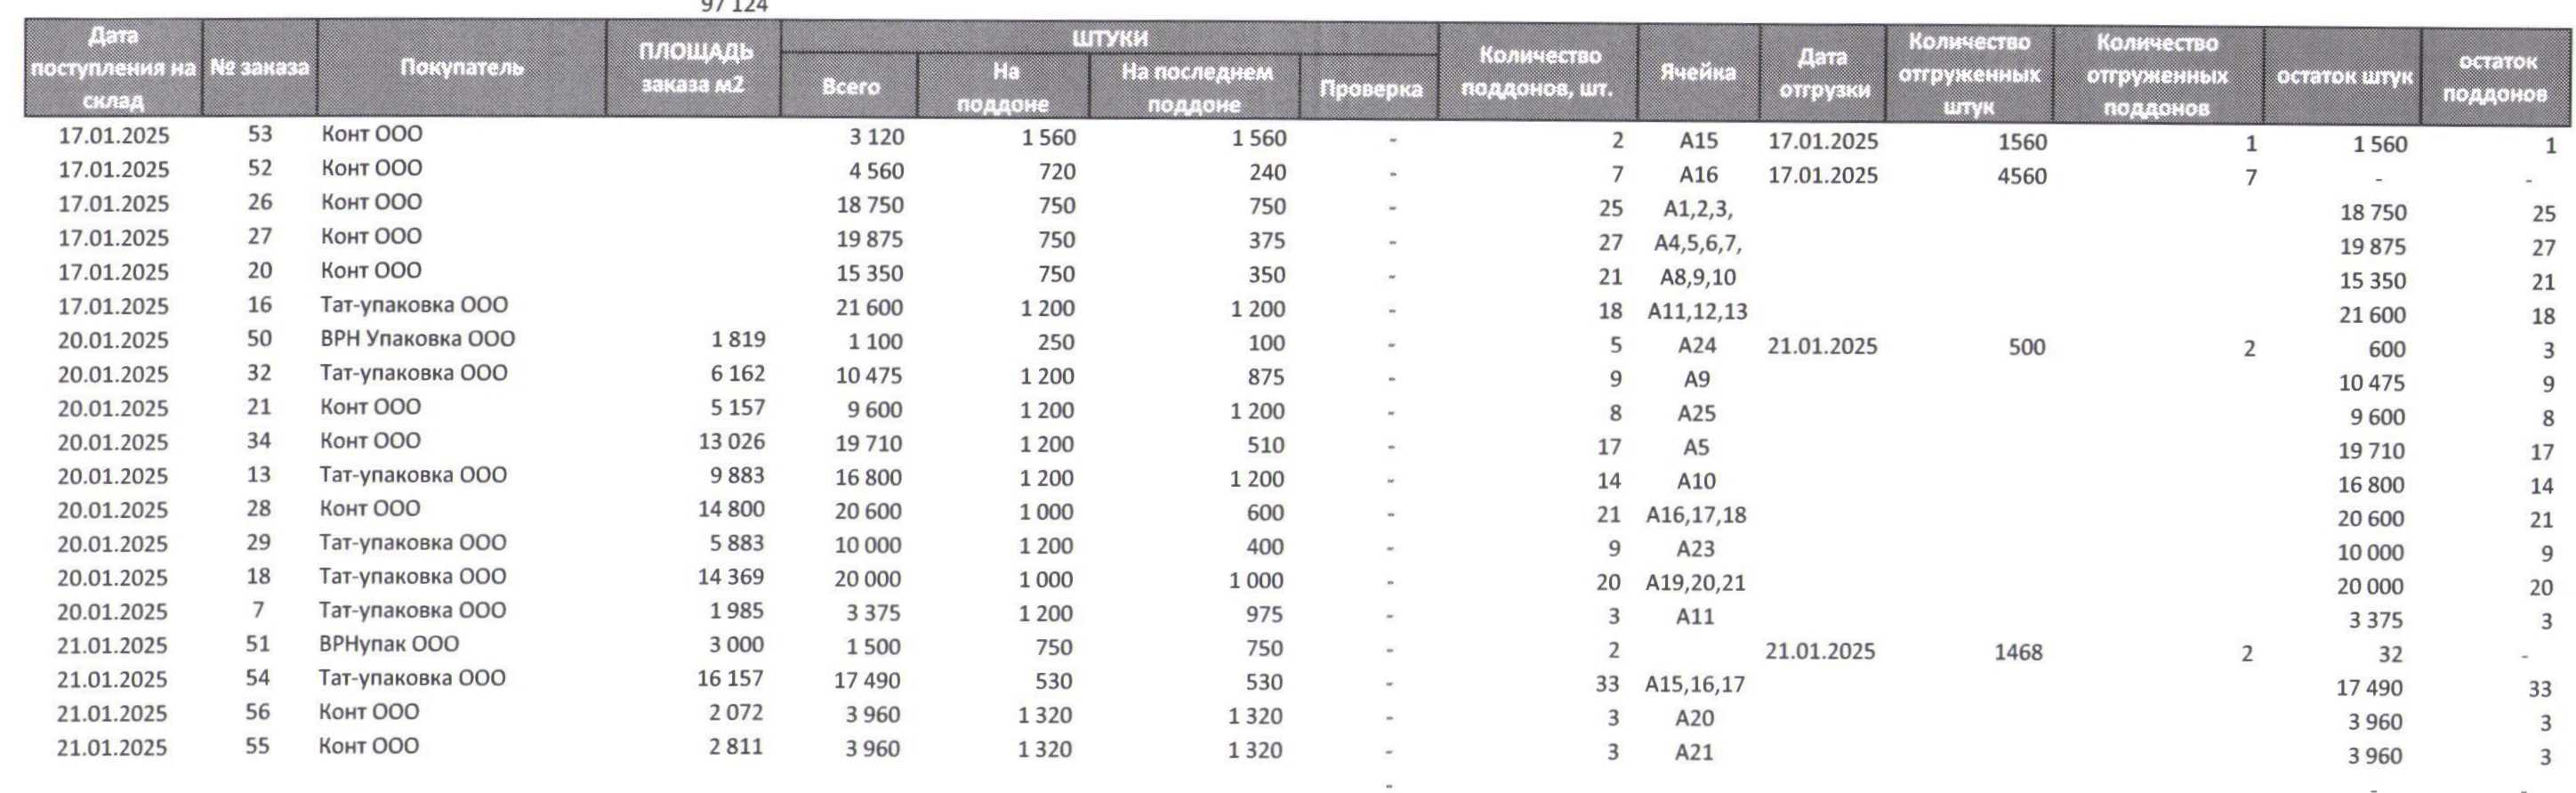
\includegraphics[width=\linewidth, height=0.94\textheight, angle=90, keepaspectratio]{Pics/f10.jpg}
\end{center}
\caption{Остатки готовой продукции на складе}
\label{pic:f10}
\end{figure}

\begin{figure}
\begin{center}
 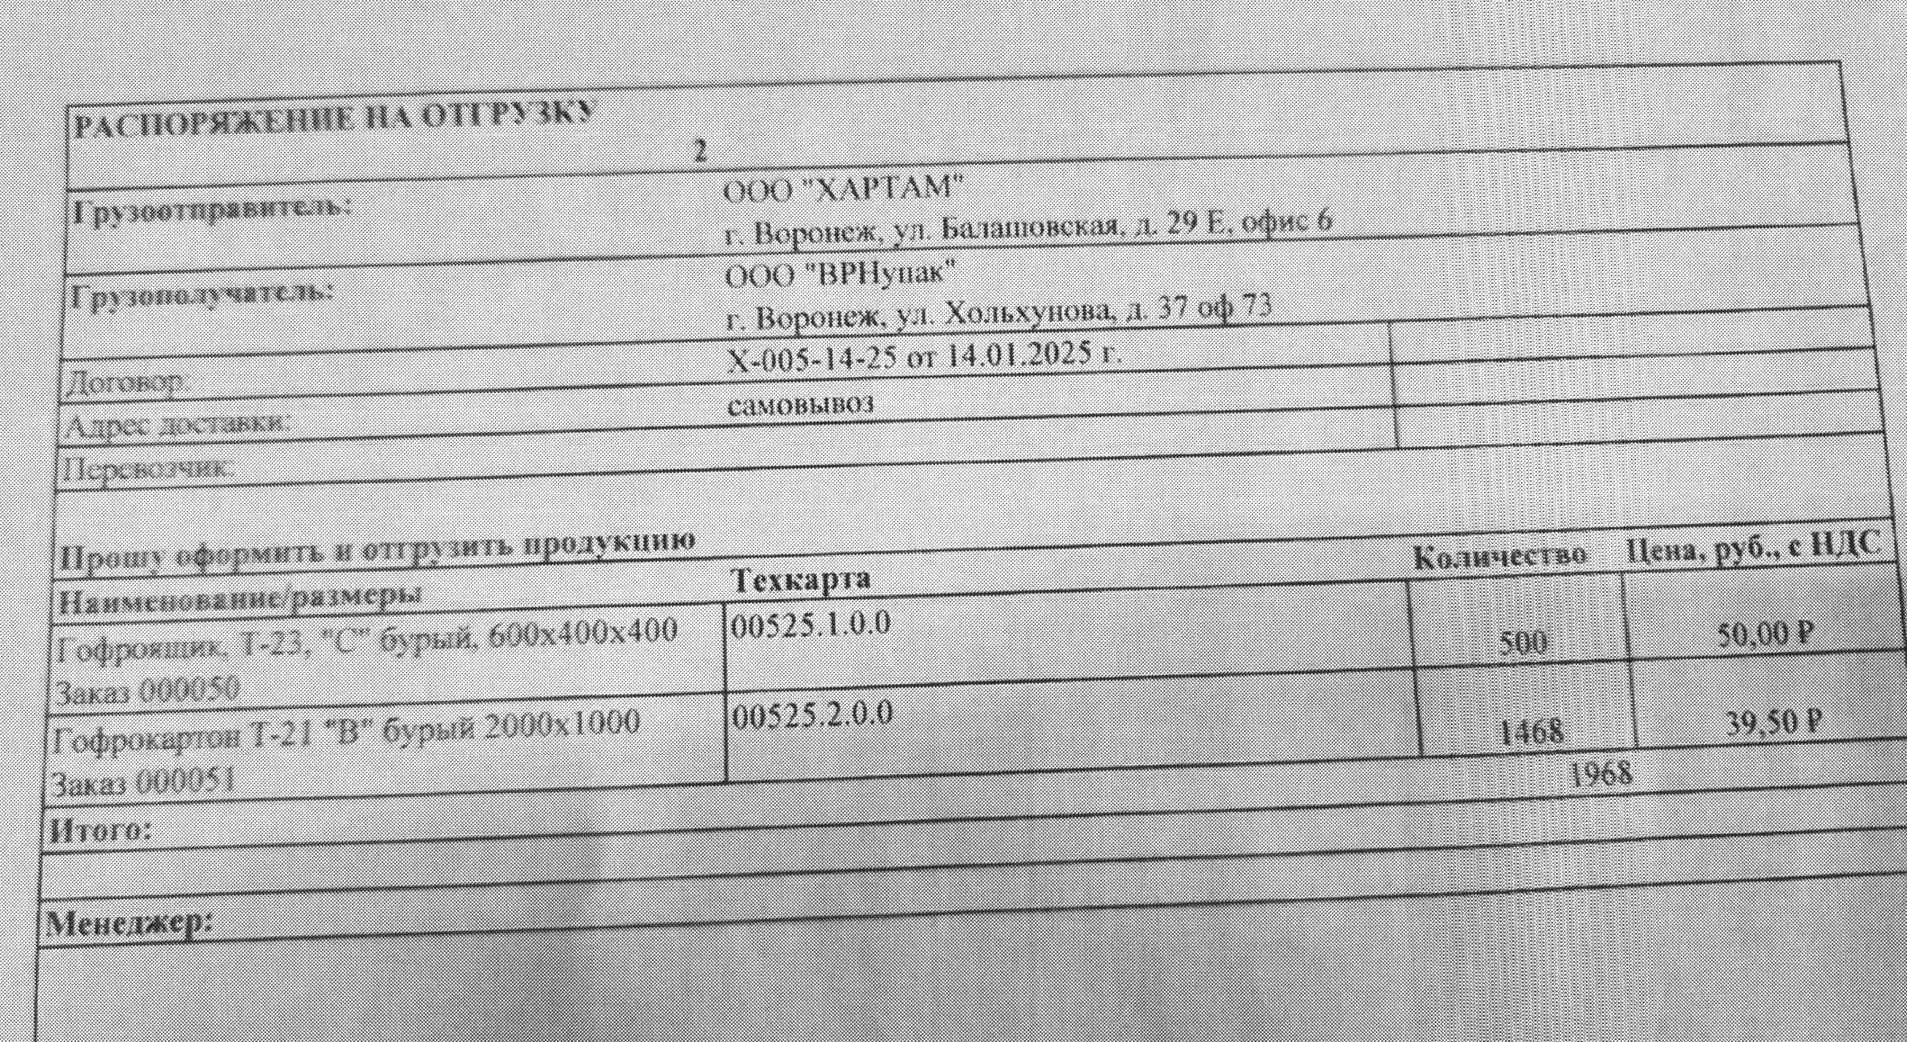
\includegraphics[width=\linewidth, height=0.94\textheight, keepaspectratio]{Pics/f11.jpg}
\end{center}
\caption{Распоряжение на отгрузку}
\label{pic:f11}
\end{figure}

\begin{figure}
\begin{center}
 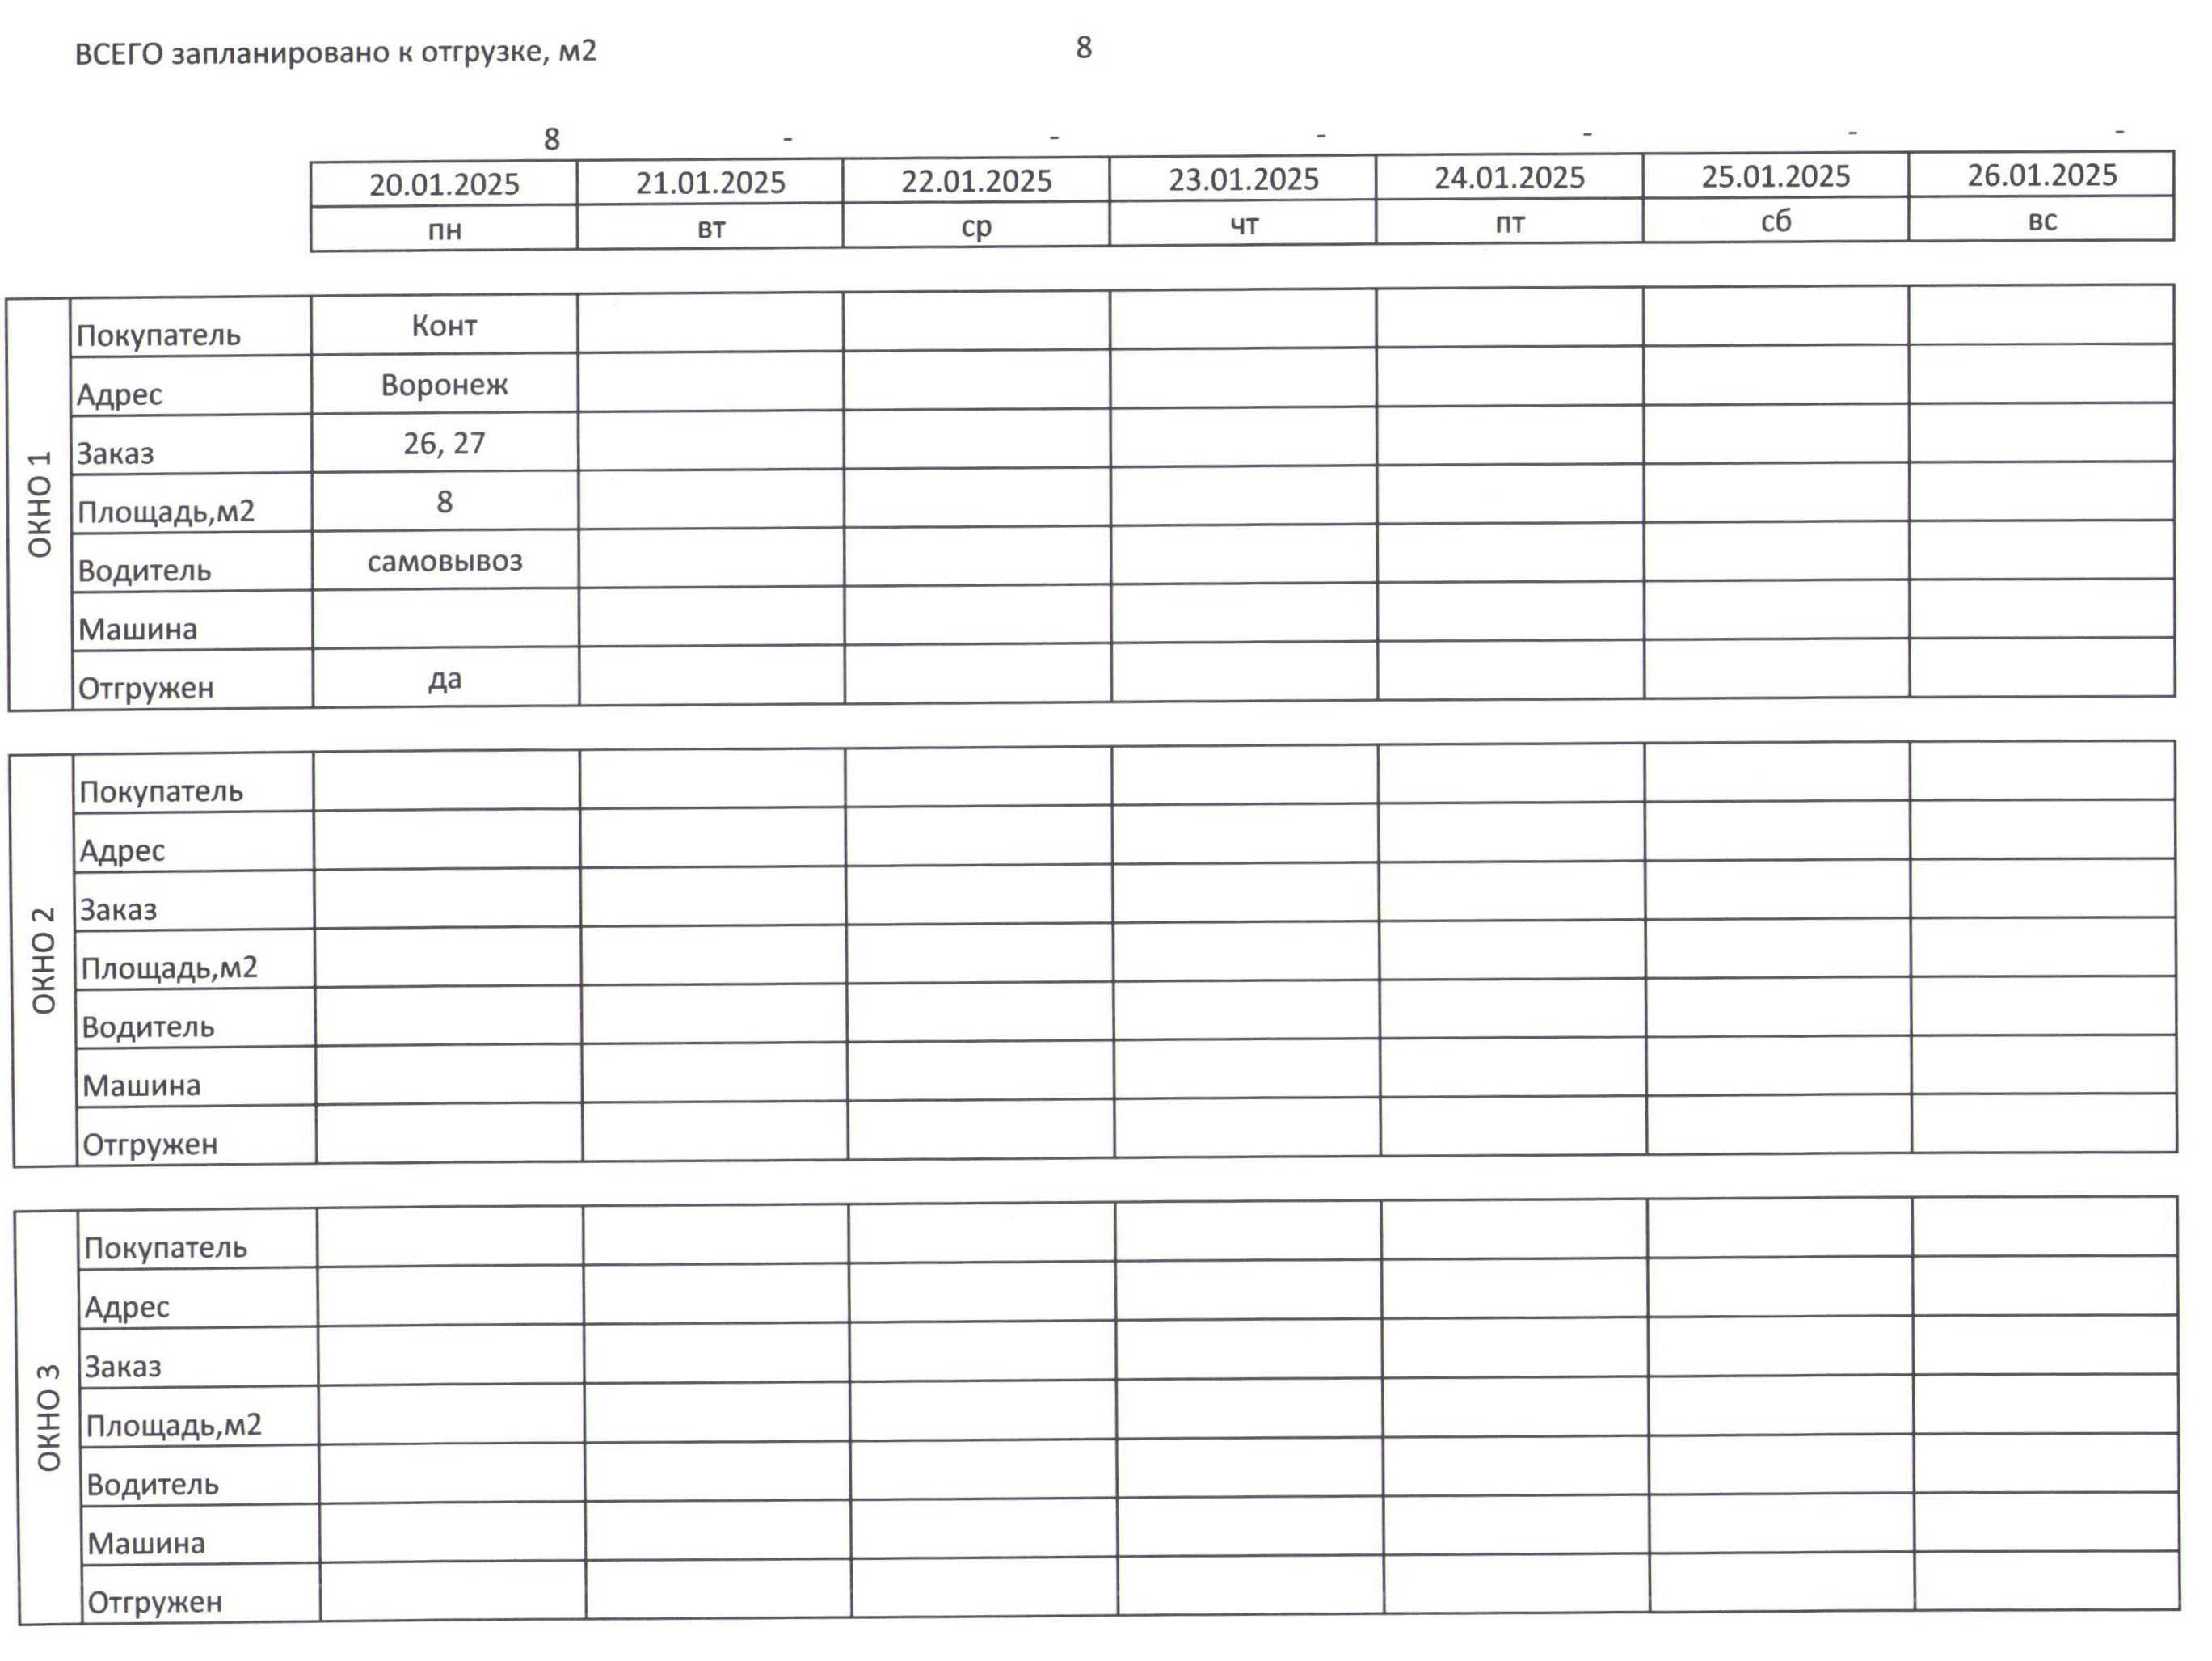
\includegraphics[width=\linewidth, height=0.94\textheight, keepaspectratio]{Pics/f14.jpg}
\end{center}
\caption{График отгрузки}
\label{pic:f14}
\end{figure}

 % Планирование отгрузки
% \newpage
\subsection{Отгрузка готовой продукции}
\label{bp:Shipment}


Менеджер создает распоряжение на отгрузку и скидывает в общий чат в WhatsApp.  Начальник склада находит транспорт и сообщает данные об автомобиле. При отгрузке на условиях самовывоза менеджер сообщает в общем чате данные водителя, вид и номер транспортного средства. Кладовщик передает данные автомобиля на охрану. 

Графика подачи машин не выявлено, машины на погрузку подъезжают в любом порядке.
О прибытии транспорта на территорию предприятия охрана информирует склад. Кладовщик связывается с водителем и сообщает ему место погрузки. 

Кладовщик выполняет погрузку готовой продукции в транспорт: находит паллеты с готовой продукцией на складе согласно документу <<Распоряжение на отгрузку>>. 
Водитель погрузчика определяет место хранения готовой продукции на основе данных таблицы  данными таблицы MS EXCEL (рис. \ref{pic:f10}). 

Водитель погрузчика грузит продукцию в транспорт. Кладовщик фиксирует факт отгрузки в копии распоряжения на отгрузку.
После погрузки кладовщик в общем чате в WhatsApp сообщает о завершении погрузки, после чего бухгалтер формирует комплект сопроводительных документов, которые передает с водителем или пересылает заказчику по электронной почте.


На предприятии ведется реестр контрагентов с указанием используемого перечня отгрузочных документов (рис. \ref{pic:f12}). 


\begin{figure}
\begin{center}
 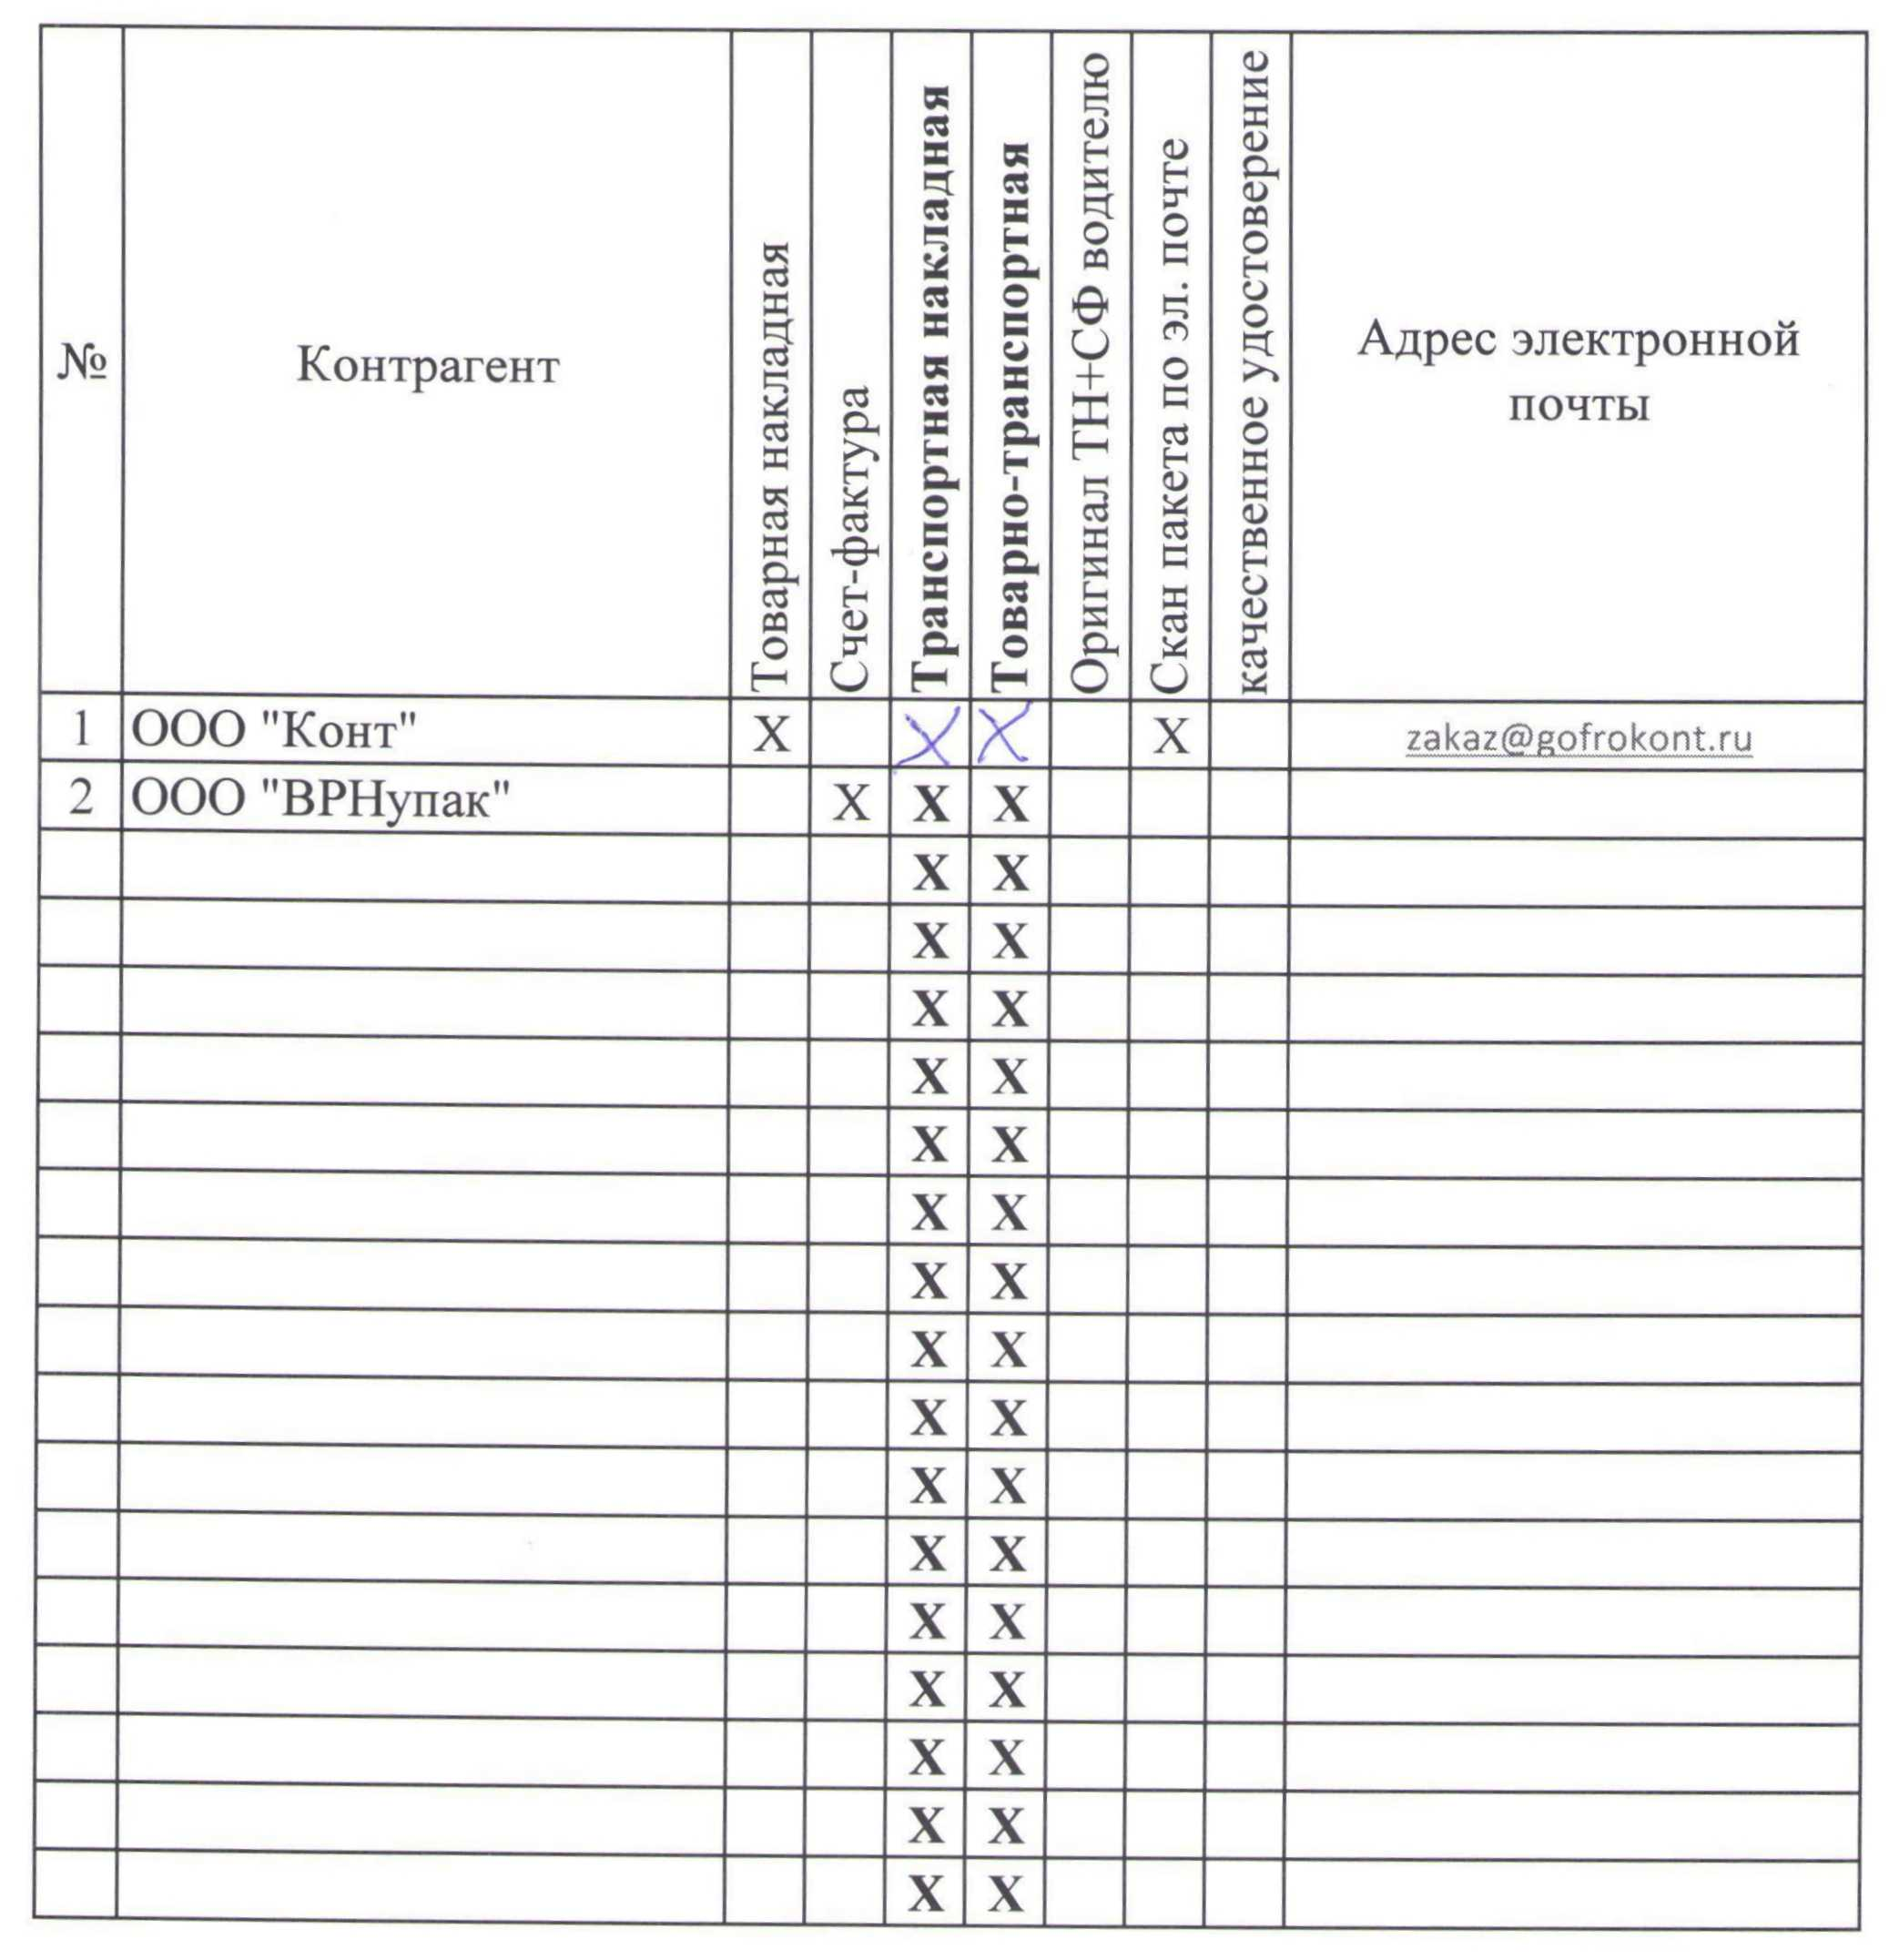
\includegraphics[width=\linewidth, height=0.94\textheight, keepaspectratio]{Pics/f12.jpg}
\end{center}
\caption{Реестр контрагентов}
\label{pic:f12}
\end{figure}

\clearpage % Отгрузка готовой продукции
% \newpage
\subsection{Планирование сырья}
\label{bp:RawMaterialPlanning}

\textbf{Планирование бумаги и картона}

Планирование основного сырья (бумага и картон) выполняется главным технологом. 

Нормативы по сырью на момент проведения аудита не разработаны. 

Основное сырье (бумага и картон) поставляется предприятием ООО ''Эколайнер''.


% \textbf{Планирование закупки заготовок}


% % \todo{перечитать с планированием}



\textbf{Планирование вспомогательных материалов}

На момент проведения аудита не регламентировано.

% Планированием и закупкой вспомогательных материалов занимается отдел снабжения.

% Каждый день техник по учету определяет остатки по крахмалу и другим материалам (Пленка, скотч и др.) в производстве и сообщает по телефону в отдел снабжения остатки на складе. 25 числа каждого месяца менеджер по снабжению заказывает поставки крахмала на следующий месяц. Объемы заказа определяются коллективно с техником по учету. Менеджер отдела снабжения обзванивает поставщиков по ценам, формирует заявку в свободной форме. Поставки крахмала выполняются 2-3 раза в месяц.

% В системе СБИС хранятся текущие остатки на складах, но отдел снабжения не использует систему СБИС.


% По закупке других материалов (СИЗ, спецодежда, комплектующие и запчасти) отдел снабжения собирает заявки от подразделений, обрабатывает их, ищет поставщиков и производит закупку.


% Поддоны.

% Начальник склада каждый вечер определяет потребность по поддонам и сообщает по телефону в отдел снабжения, где менеджеры отдела снабжения фиксирует вручную объемы потребности.
% Коммерческий отдел и отдел снабжения совместно определяют потребность в поддонах исходя из плана производства и текущих остатков на складах и заказывают поддоны у производителей.
% Менеджеры отдела снабжения создают заявку на закупку поддонов и спецподдонов. Все поддоны невозвратные.
% Поддоны принимаются на складе. Учет поступления фиксируется в системе СБИС.


\textbf{Планирование краски }

На момент проведения аудита не регламентировано.





\clearpage
\ifx \notincludehead\undefined
\normalsize
\end{document}
\fi % Планирование сырья
% %\newpage
\subsection{Оперативное планирование производства}
\label{bp:OperPlan}


Все заявки от покупателей менеджер отдела продаж регистрирует в таблице MS EXCEL.




\textbf{Планирование работы гофроагрегата}

Главный технолог используя шаблон в таблице MS EXCEL кроит (осуществляет поиск подкроя по ширине гофрополотна на гофроагрегате)  задания на гофроагрегат вручную. 

Утверждено несколько марок выпускаемого картона. Композитный состав не утвержден.



\textbf{Планирование линий переработки}

Главный технолог создает план на переработку вручную по каждой производственной линии в таблице MS EXCEL %\ref{pic:d4}.

Главный технолог печатает задание на линию и передает мастеру производства. 
Мастер производства при получении плана работы самостоятельно распределяет задания по линиям исходя из загруженности производственных мощностей.
Задания передаются операторам линий переработки. 



\clearpage

\ifx \notincludehead\undefined
\normalsize
\end{document}
\fi % Оперативное планирование производства
% %\newpage
\subsection{Подготовка производства}
\label{bp:Prepare}
%

Единая форма для сбора входящей информации (опросный лист) отсутствует.
Заказчик присылает требования на изготовления продукции в произвольной форме.

Обработка запроса может производиться на основании образец продукции, предоставленного заказчиком. Полученный от заказчика образец изделия из гофрокартона передается дизайнеру, который производит измерение размеров. Дизайнер производит расчет размеров требуемого изделия из гофрокартона в случае, если заказчик в качестве образца передал упаковываемый товар.

От менеджера дизайнерам поступает заявка (рис. \ref{pic:f16}), где прописываются требования к изделиям. 

Дизайнер переносит данные вручную в шаблон ТК, разработанный в MS EXCEL. Часть данных просчитывается по формуле. Параметры без формул  рассчитываются вручную. Технологическая карта разрабатывается в виде таблицы в MS EXCEL (рис. \ref{pic:f15}).

При разработке технологической карты для изделия, производимого с использованием штампа, менеджер передает в отдел дизайна макет штампа. 
После обработки макет отправляется главному технологу. Главный технолог чертит принимает решение о количестве мест на штампе и информацию передает в виде карандашного рисунка, сделанного своей рукой.
Главный технолог разрабатывает маршрут изготовления ГП. 
После внесения корректировок в ТК, производимых главным технологом, ТК возвращается дизайнерам. Далее дизайнеры отсылают готовый макетом поставщику штампов, размещают заказ на изготовление.

При разработке дизайна менеджер передает дизайнерам эскиз печати. Этот эскиз обрабатывают и передают поставщику клише для изготовления оснастки. 

После создания технологической карты дизайнер отправляет ее на согласование главному технологу. Только после согласования главным технологом ТК направляют менеджеру отдела продаж для утверждения заказчиком. 
  
При необходимости выкрасов дизайнер совместно с колористом определяют номер оттенка по шкале Pantone. Номер кода цвета отсылают в Москву в компанию <<АГ Флекс>>, откуда приходит формула цвета, по которой смешивают краску и делают выкрасы вручную.

Номер технологической карты присваивают дизайнеры.


Готовые технологические карты хранят на сервере в виде таблиц MS EXCEL. К ним имеют доступ все заинтересованные лица без возможности внесения изменений.

При внесении в уже действующую технологическую карту изменений дизайнеры создают новую ТК, которой присваивается новый номер.


\begin{figure}
\begin{center}
 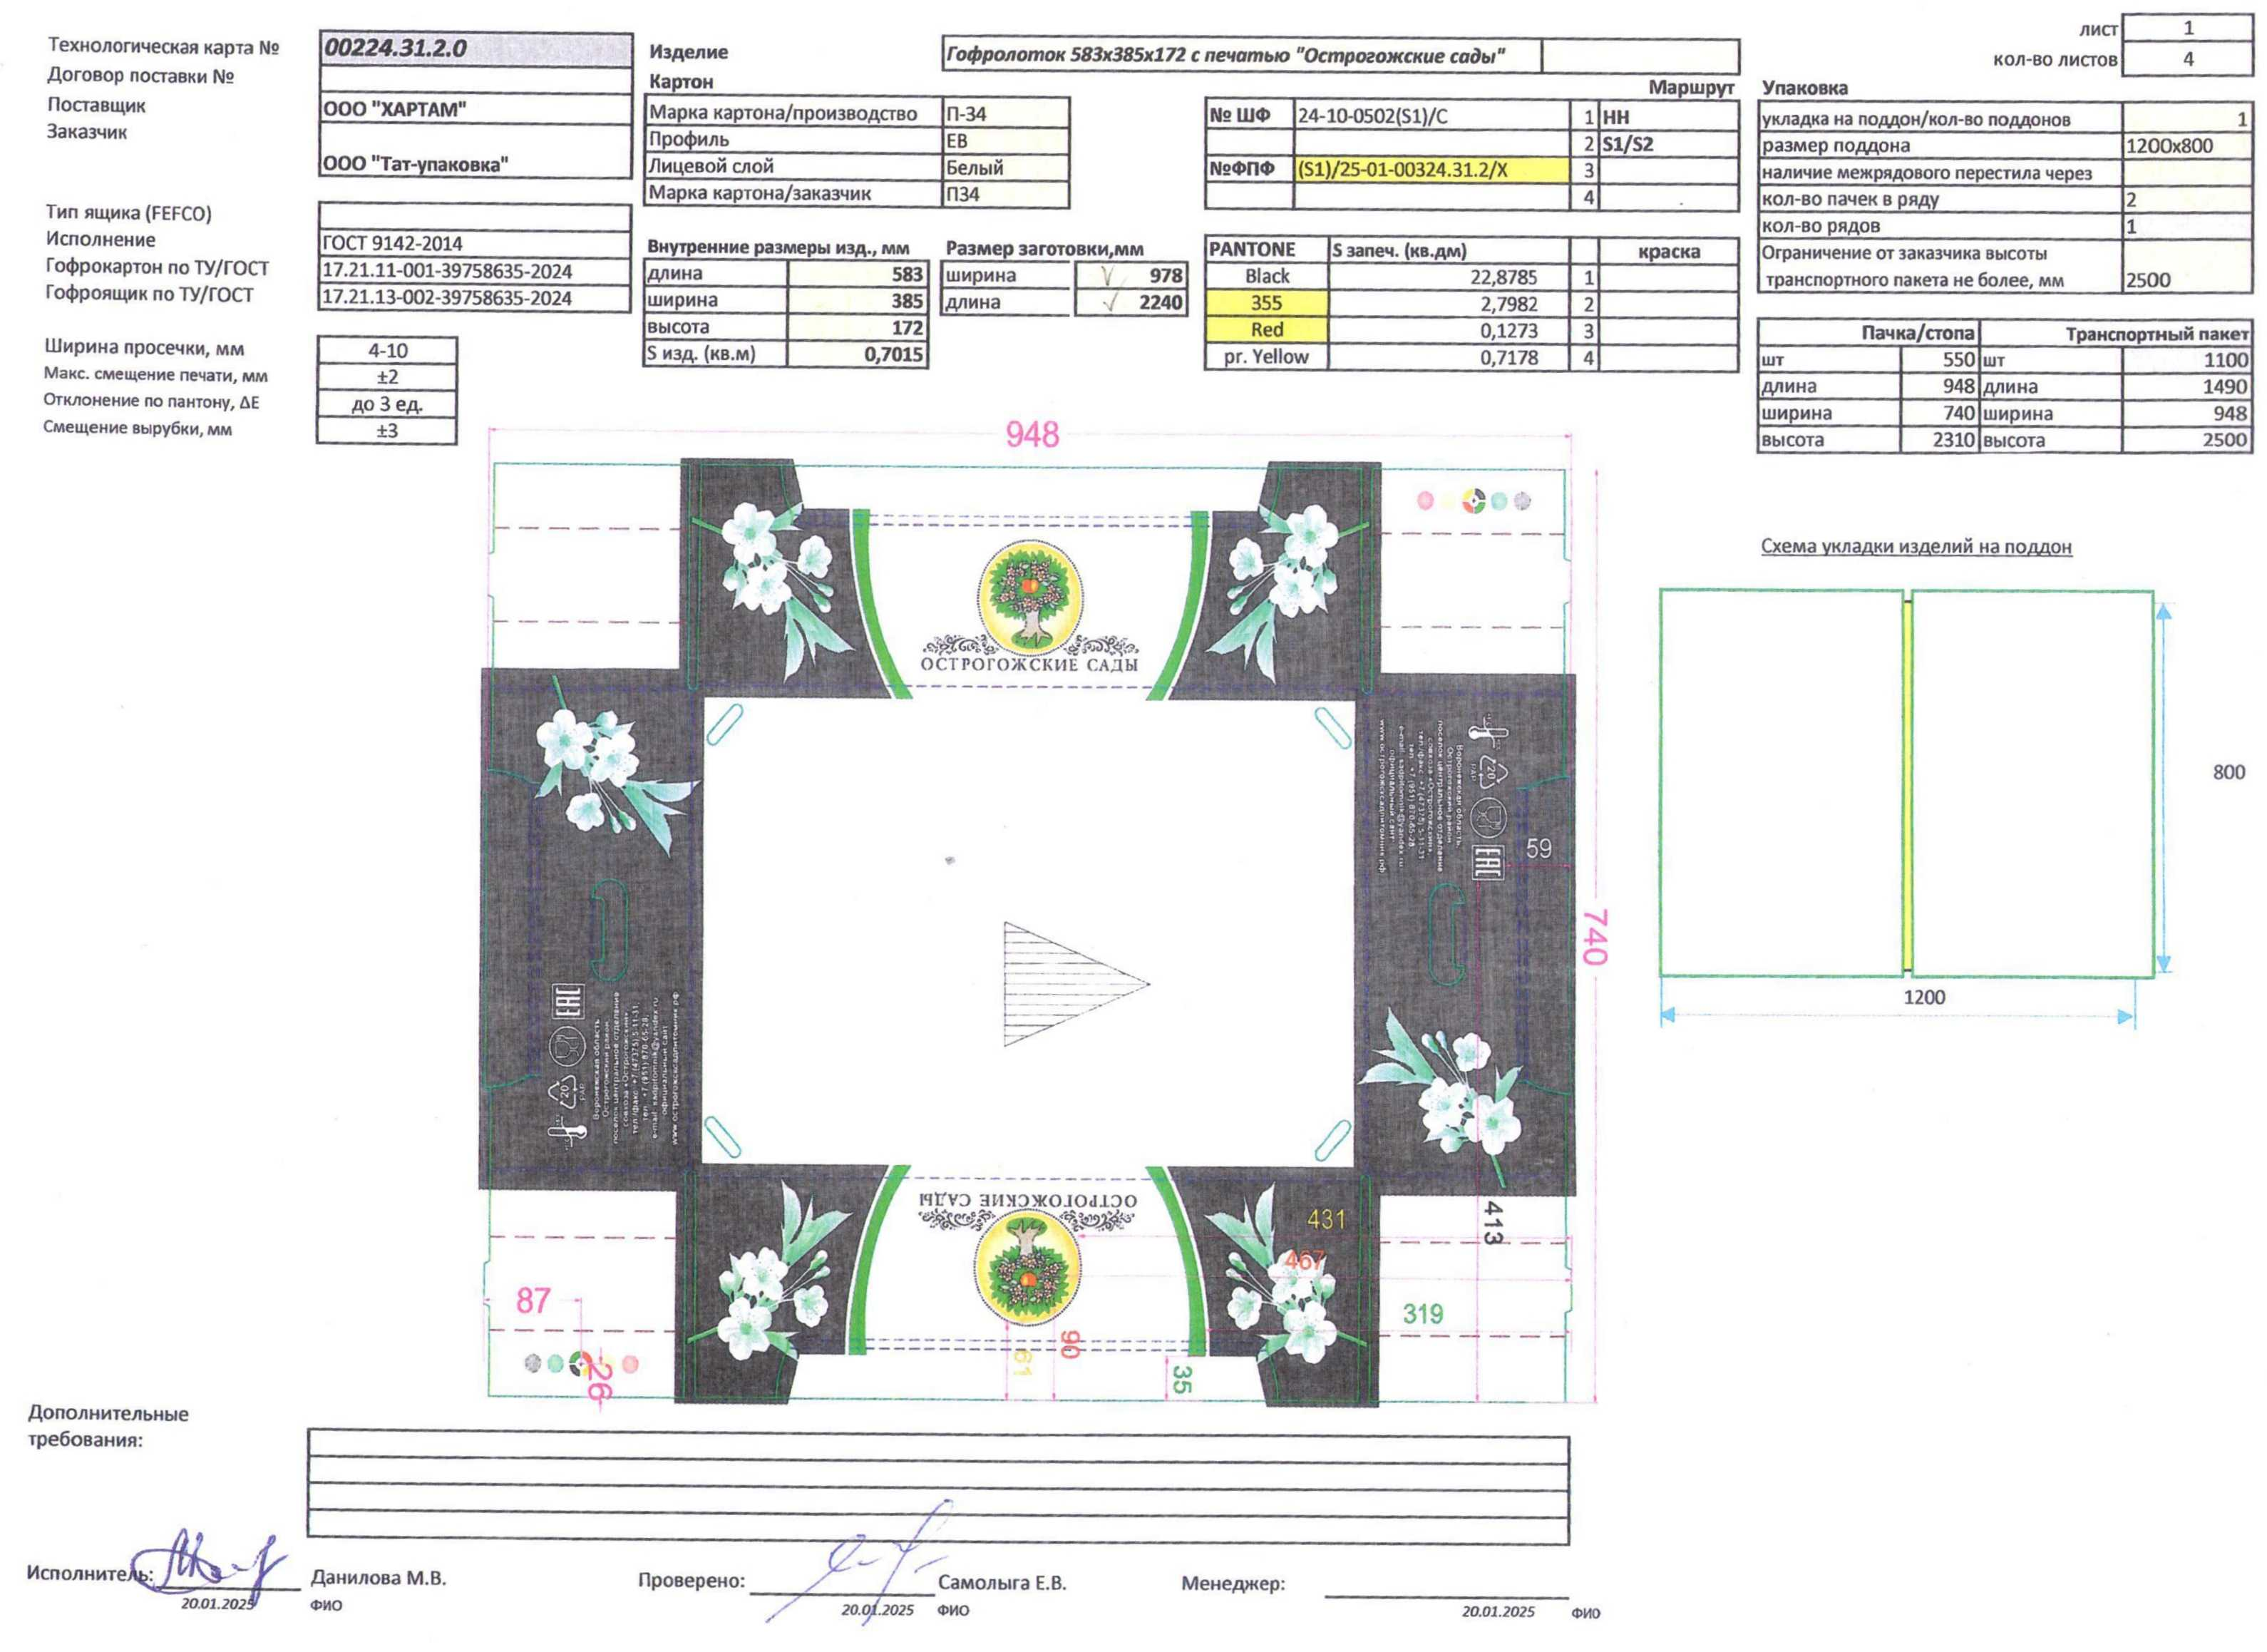
\includegraphics[width=\linewidth, height=0.94\textheight, angle=90, keepaspectratio]{Pics/f15.jpg}
\end{center}
\caption{Разработка ТК}
\label{pic:f15}
\end{figure}

\begin{figure}
\begin{center}
 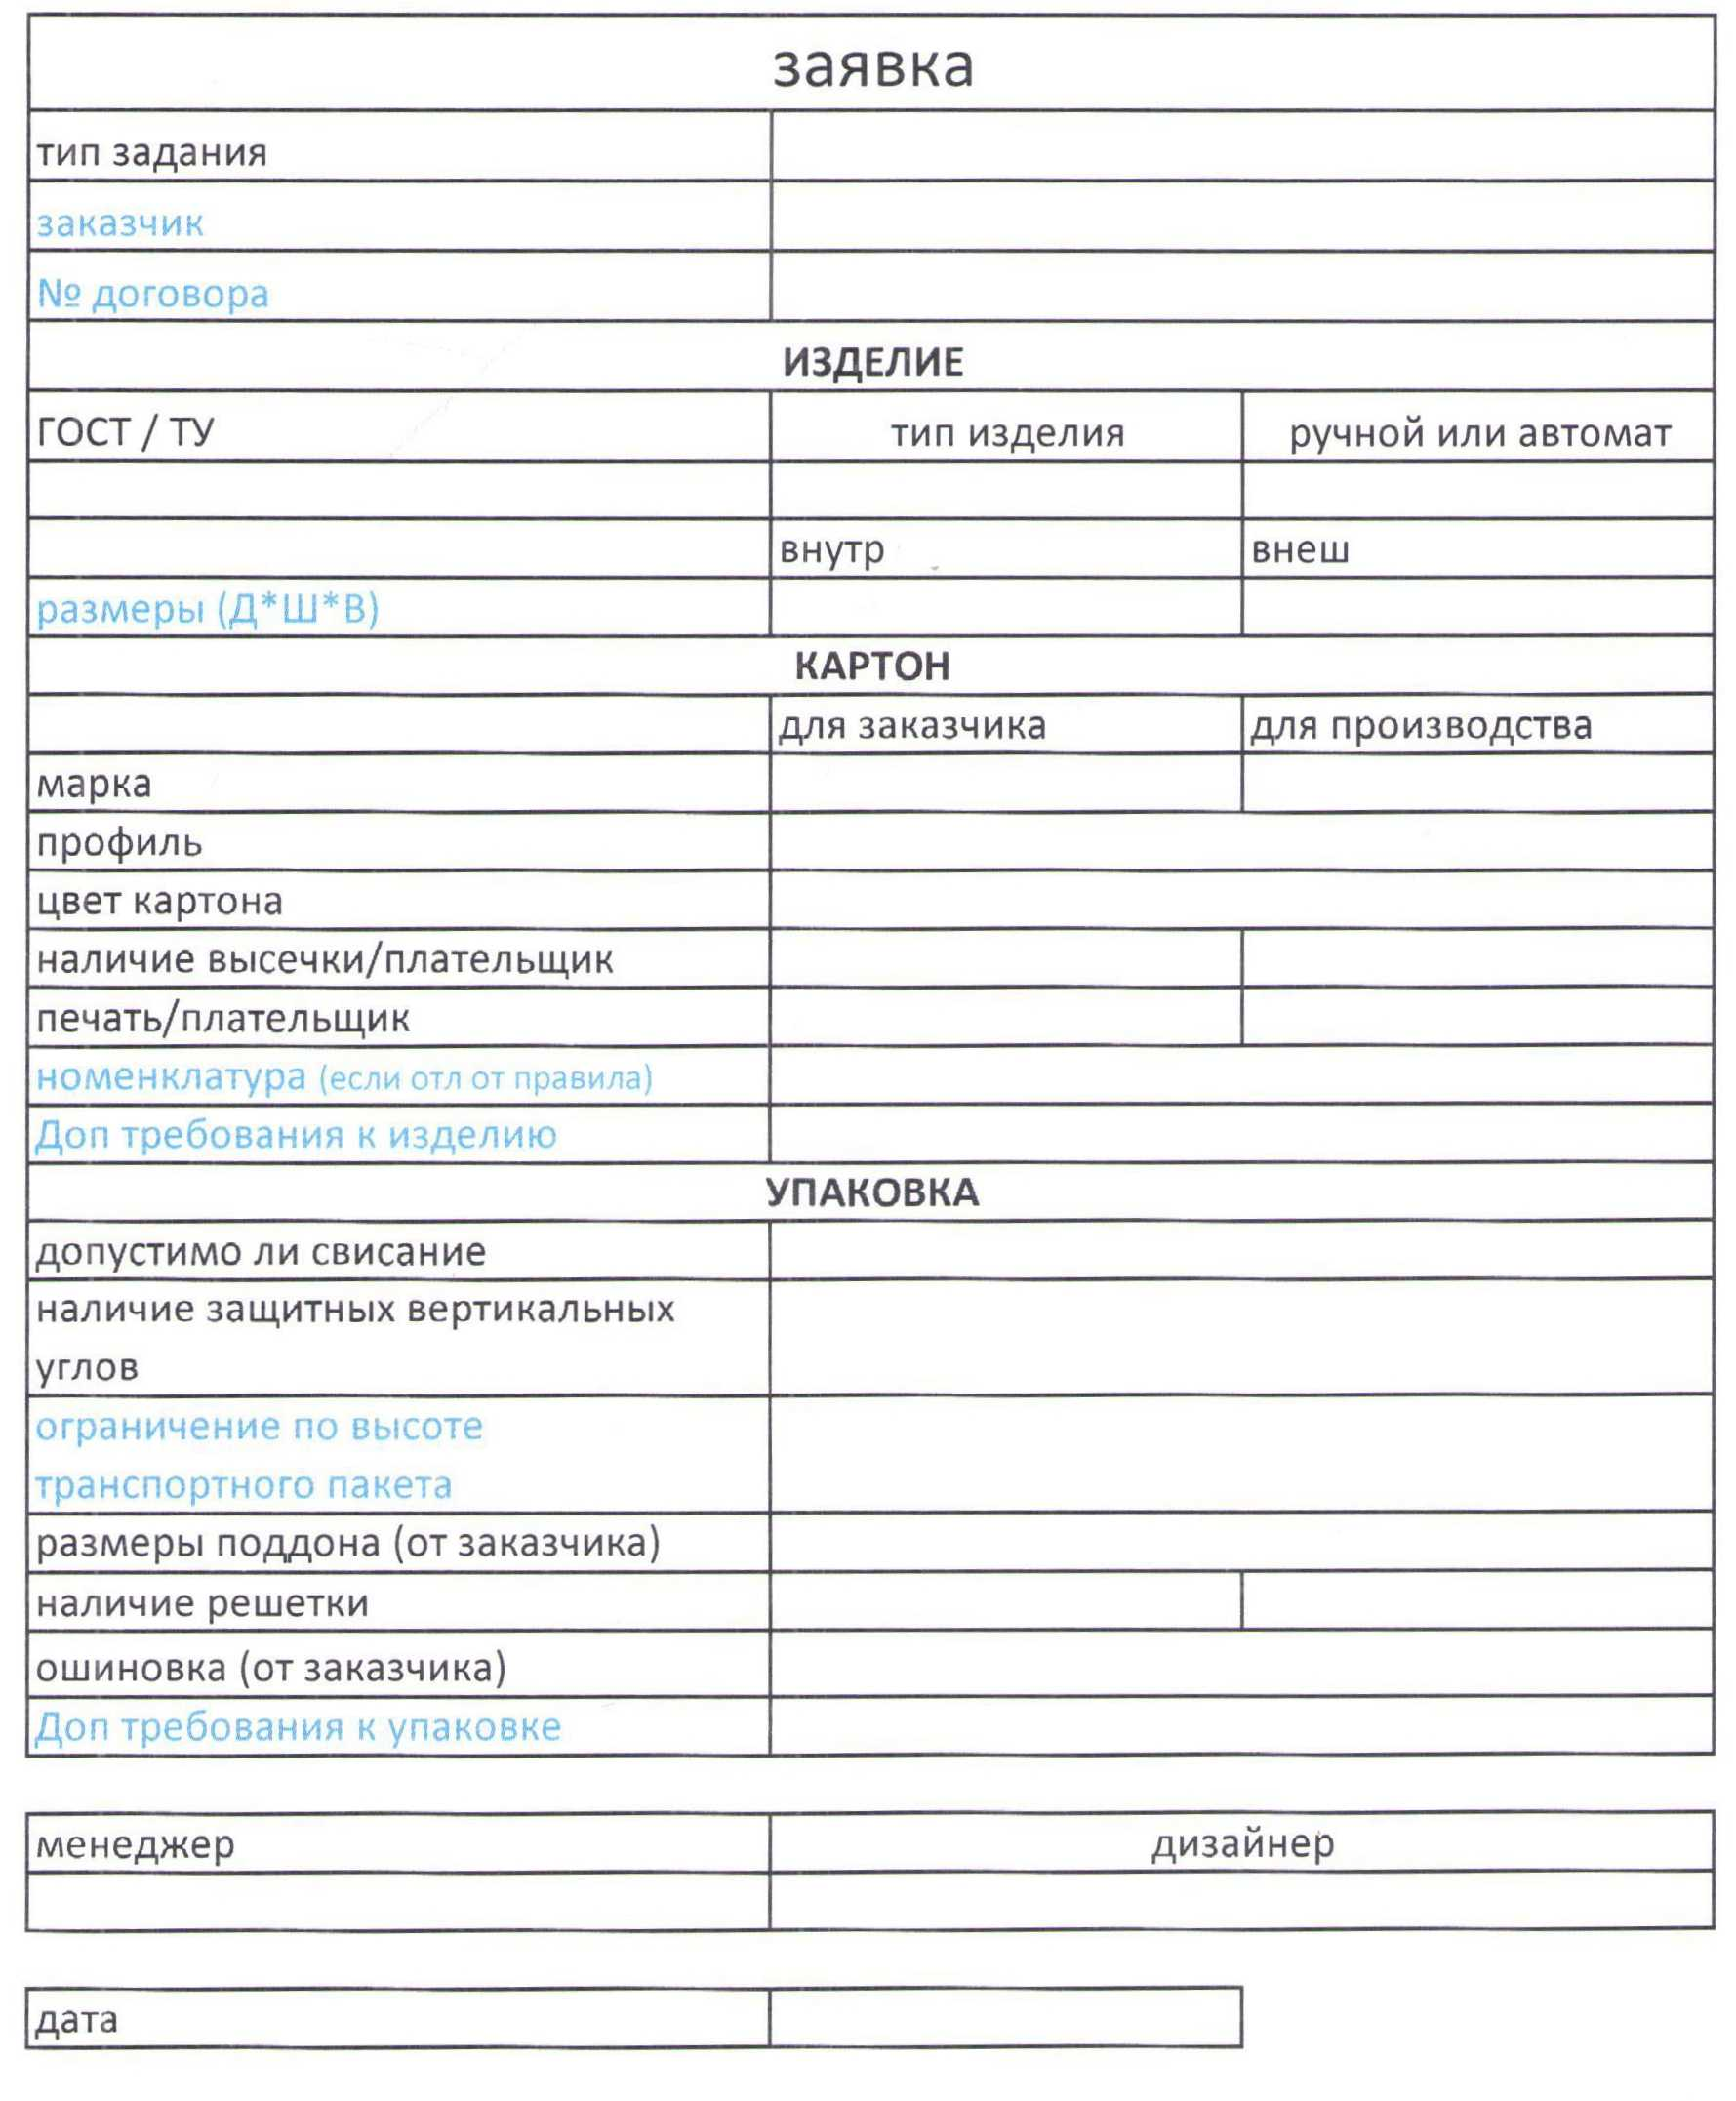
\includegraphics[width=\linewidth, height=0.94\textheight, keepaspectratio]{Pics/f16.jpg}
\end{center}
\caption{Заявке на разработку чертежа и макета}
\label{pic:f16}
\end{figure}
%\end{figure}


\clearpage
\ifx \notincludehead\undefined
\normalsize
\end{document}
\fi % Подготовка производства
% \newpage
\subsection{Учет технологической оснастки и краски }
\label{bp:rigging}
%
Технологическая оснастка необходима для изготовления готовой продукции. На предприятии заказывают оснастку у сторонних производителей.

При получении требований от клиента менеджер определяет необходимость использования оснастки при производстве продукции. 

Возможность изготовления нового изделия, в соответствии с техническими параметрами оборудования, определяет главный технолог. 




\textbf{Учет клише}

Дизайнер, на основании разработанного и согласованного дизайна заказывает изготовление клише. 

Предприятие использует одного поставщика клише. 
Для размещения заказа на изготовление клише дизайнер отправляет макет по электронной почте.

Учет количества размещенных заявок на изготовление клише не ведется. 
При изготовлении клише за счет клиента менеджер создает запрос в бухгалтерию для выставления счета. Бухгалтер выставляет счет на изготовление оснастки.

При поступлении на производство клише проверяется на соответствие макету, фиксируется дата поступления в MS EXCEL (рис. \ref{pic:f17}). Кладовщики о факте поступлении оснастки сообщают дизайнерам. 

Номер клише присваивает дизайнеры в момент заказа у поставщика.

На предприятии выделен участок для хранения клише.


\textbf{Учет штанцевальных форм}

 Менеджер передает в отдел дизайна макет штампа. Далее данный макет обрабатывается и отсылается главному технологу. Главный технолог чертит раскладку на штампе и прописывает оборудование, возвращает дизайнерам. Далее дизайнеры отсылают раскладку с макетом поставщику штампов и заказываю штамп.

Компания-изготовитель оснастки выставляет счет. Если изготовление штанцевальной формы выполняется за счет клиента, то менеджер делает запрос в бухгалтерию на выставление счета. Бухгалтер выставляет счет покупателю.

При поступлении штампа на производство  штамп проверяется. 

Номер присваивают дизайнера в момент заказа.

На предприятии места для хранения штампов оборудованы рядом с перерабатывающими линиями. Предусмотрена ячеистая система хранения. 

Учет штанцевальных форм ведется MS EXCEL, где указывается номер штампа и номер ячейки хранения (рис. \ref{pic:f22}).

Ремонтом оснастки занимаются в основном на производстве. Учет объема выполненных ремонтных работ не ведется.


Журнала выдачи оснастки не обнаружено.




%\subsubsection{Учет печатных форм}




%\subsubsection{Изготовление штампов}




\textbf{Учет краски}

Колорист получает задание на смену для каждой отдельной линии (рис. \ref{pic:f18}), подбирает технологические карты, по которым определяет номера краски, планируемой в работу. Колорист <<по своему опыту>> готовит краску на заказ (рецептура используется номинально). 

После приготовления краску выдают на линию. Учет краски колорист ведет в MS EXCEL (рис. \ref{pic:f19} - рис. \ref{pic:f20}). Общий итог расхода определяется по таблице MS EXCEL (рис. \ref{pic:f21}).

\begin{figure}
\begin{center}
 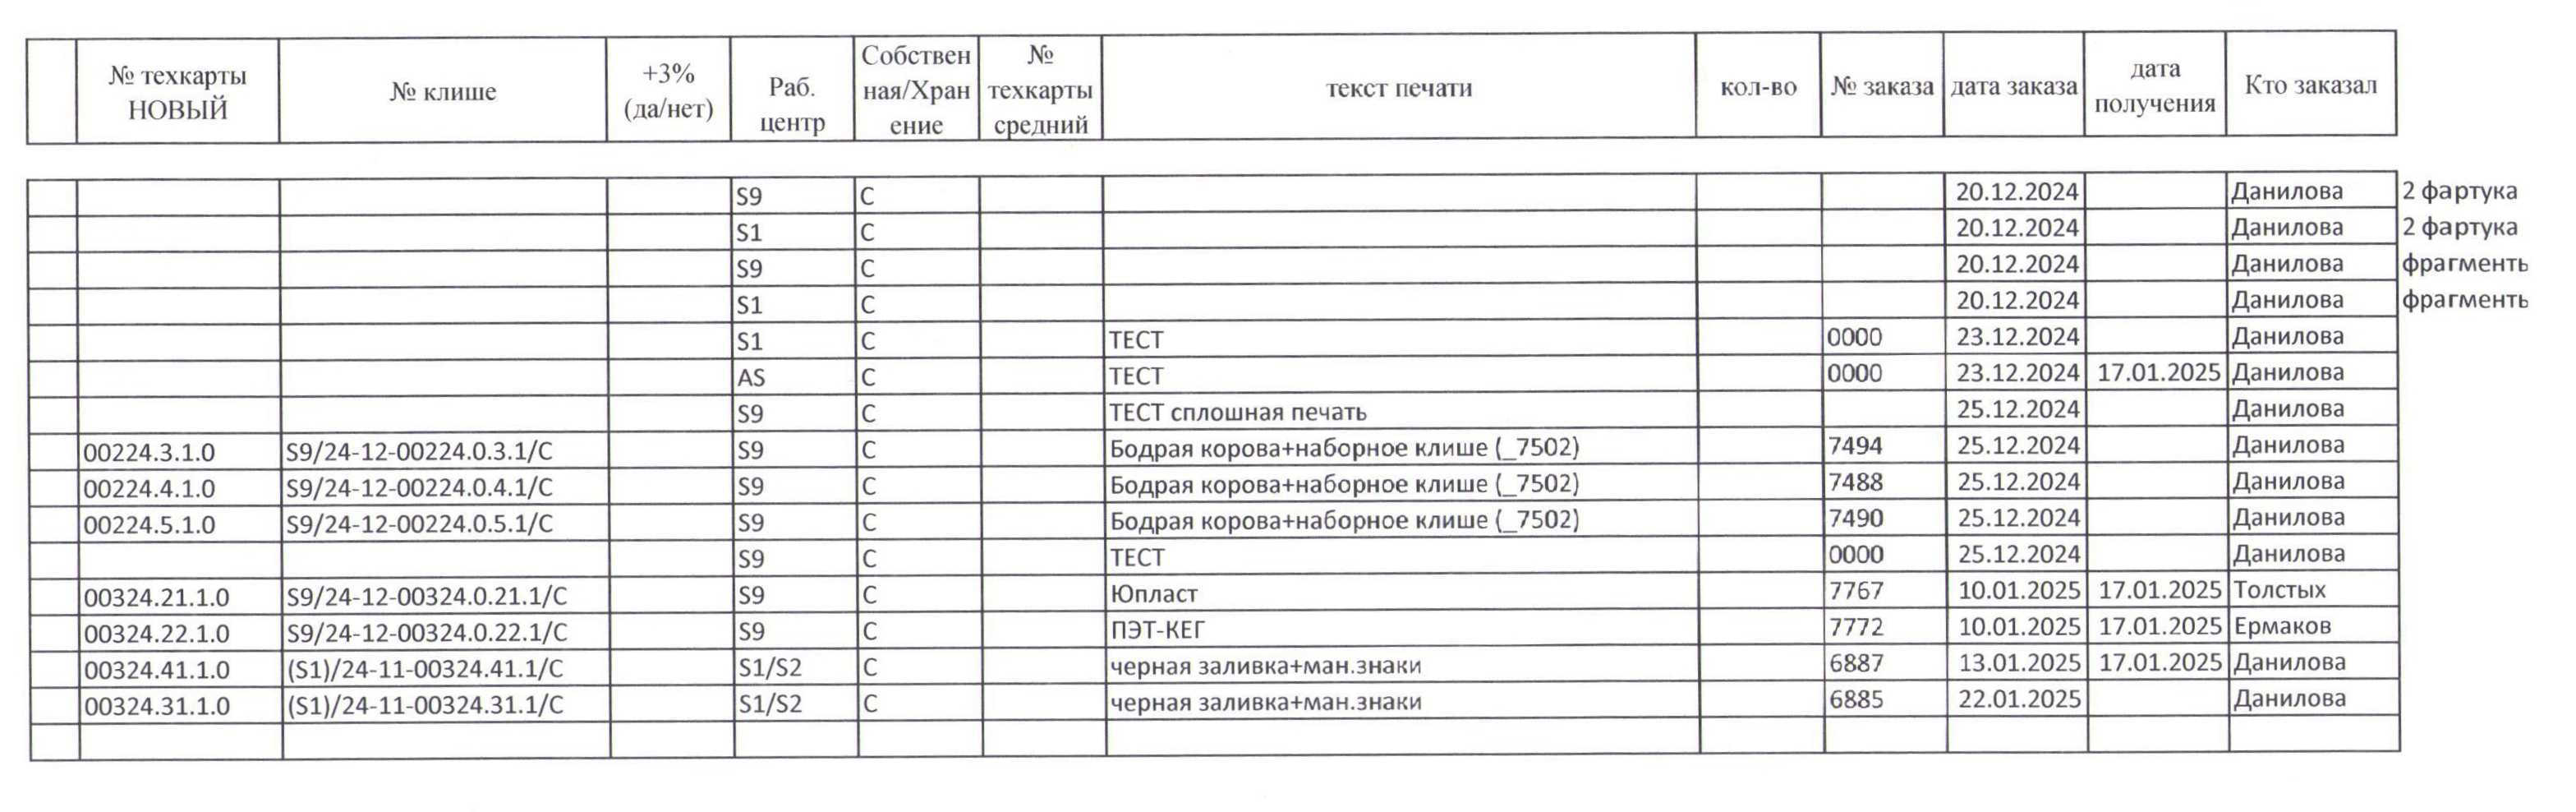
\includegraphics[width=\linewidth, height=0.94\textheight, angle=90, keepaspectratio]{Pics/f17.jpg}
\end{center}
\caption{Электронный реестр клише}
\label{pic:f17}
\end{figure}

\begin{figure}
\begin{center}
 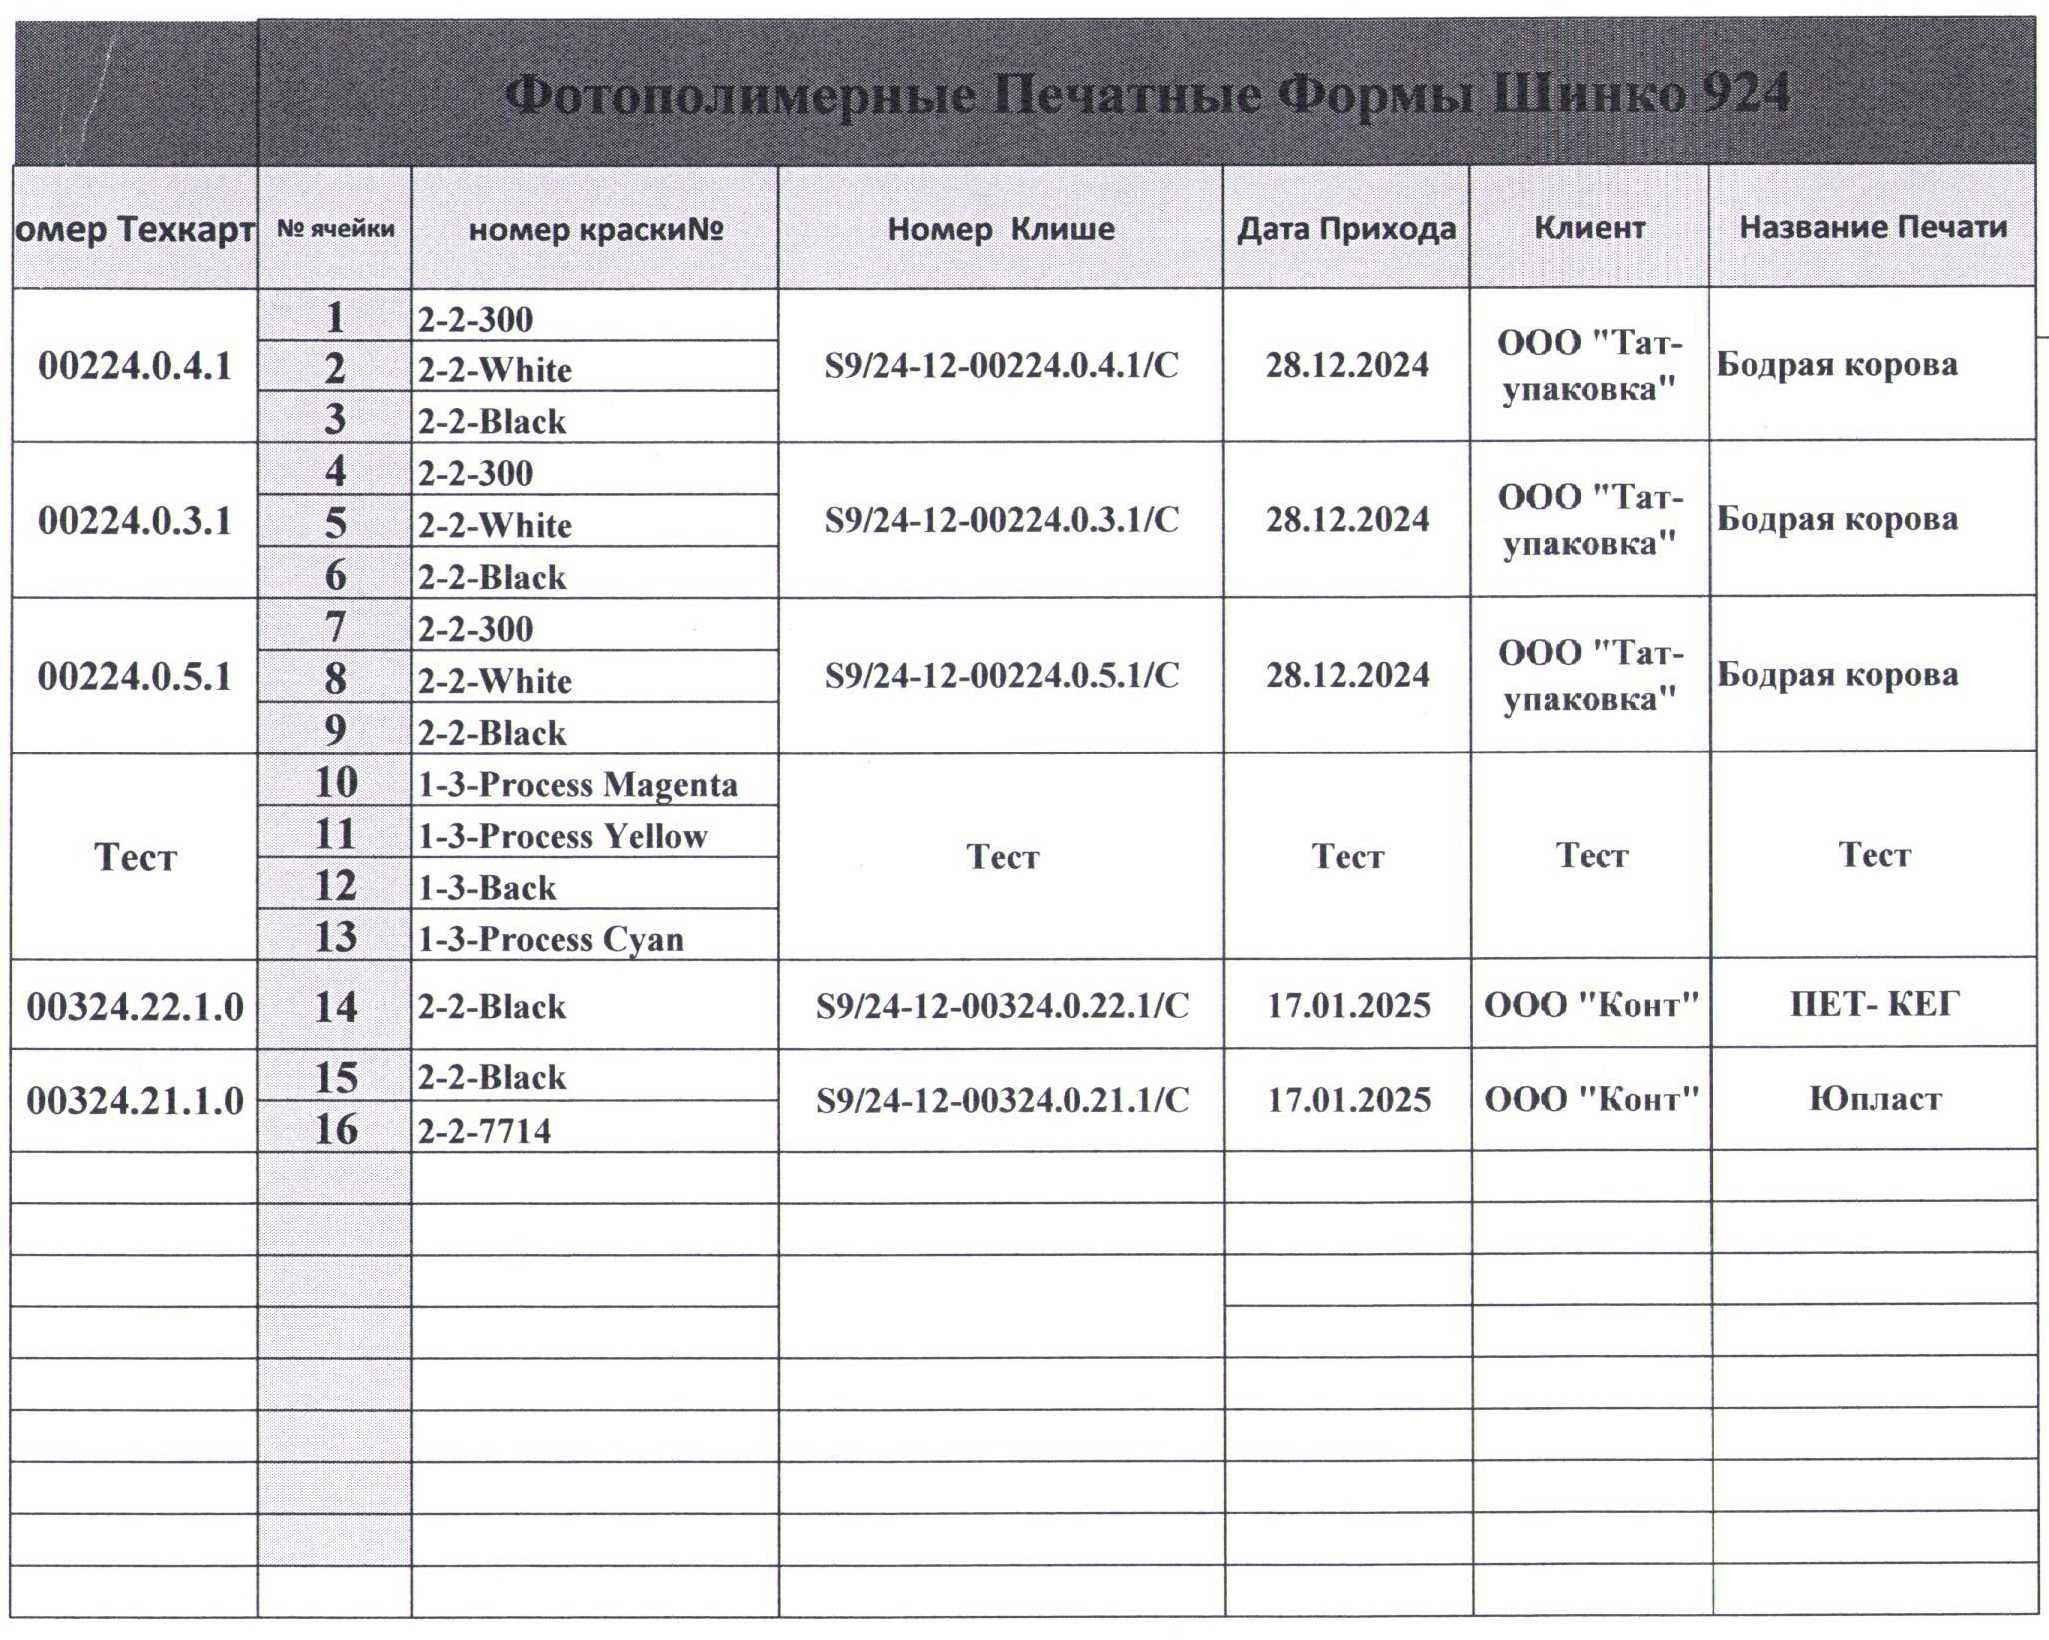
\includegraphics[width=\linewidth, height=0.94\textheight, keepaspectratio]{Pics/f22.jpg}
\end{center}
\caption{Каталог размещения клише в ячейках}
\label{pic:f22}
\end{figure}

\begin{figure}
\begin{center}
 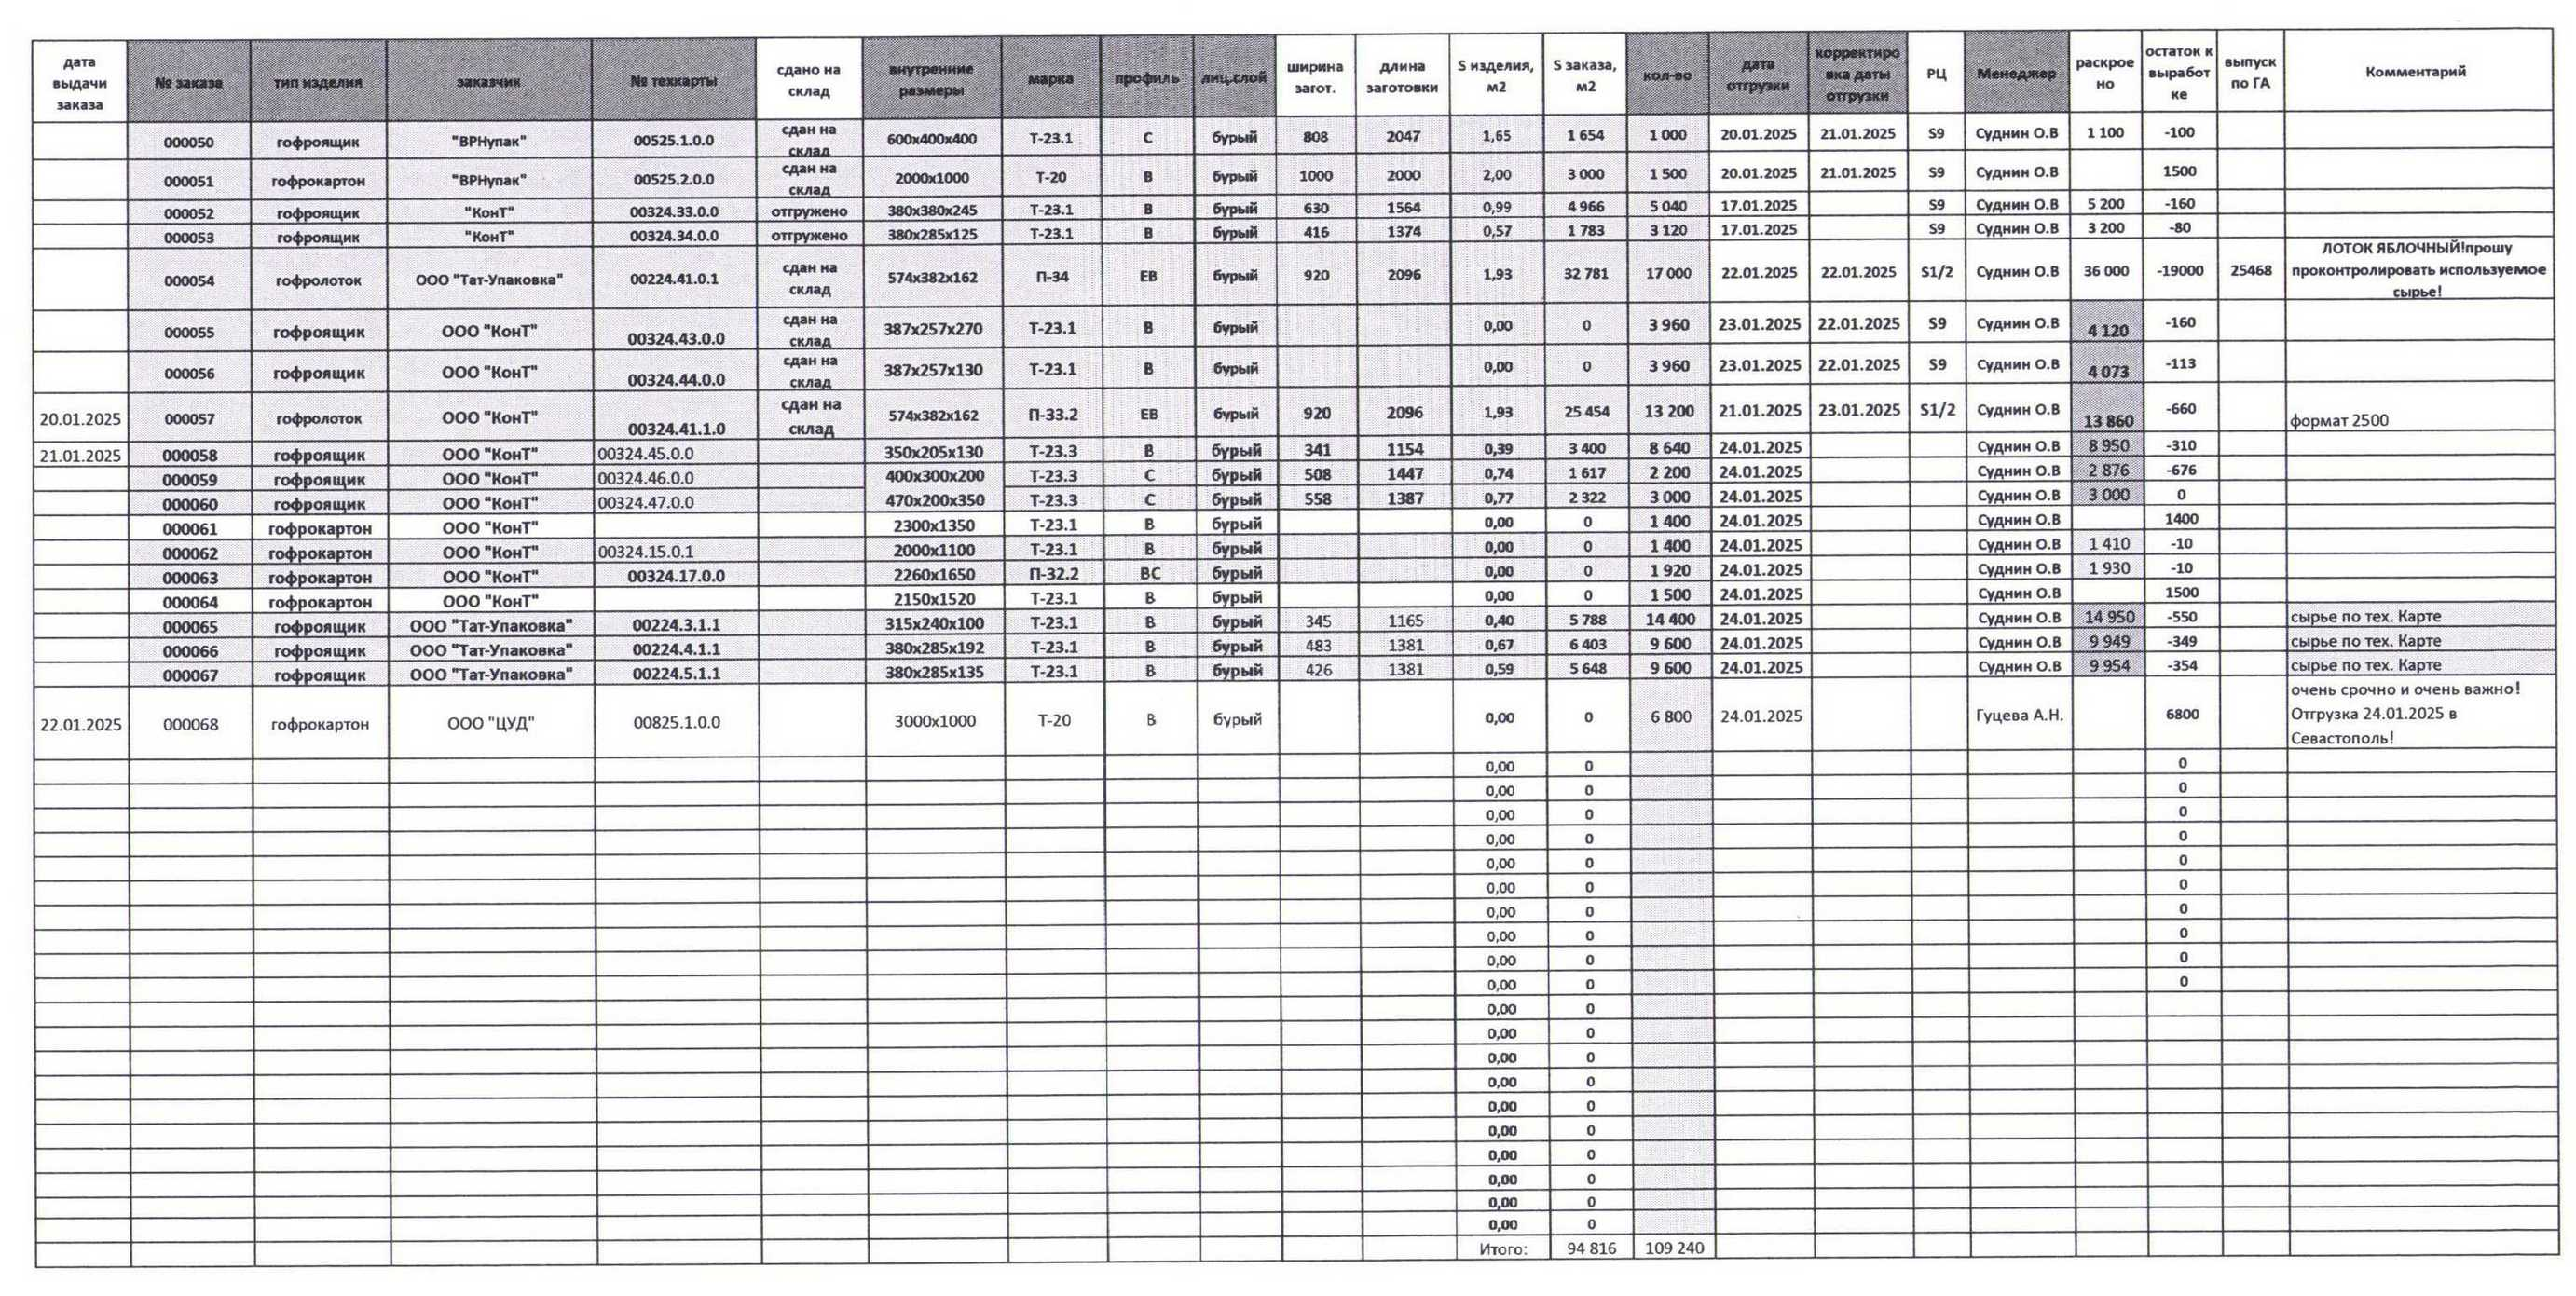
\includegraphics[width=\linewidth, height=0.94\textheight, angle=90, keepaspectratio]{Pics/f18.jpg}
\end{center}
\caption{Задание на смену для колориста}
\label{pic:f18}
\end{figure}

\begin{figure}
\begin{center}
 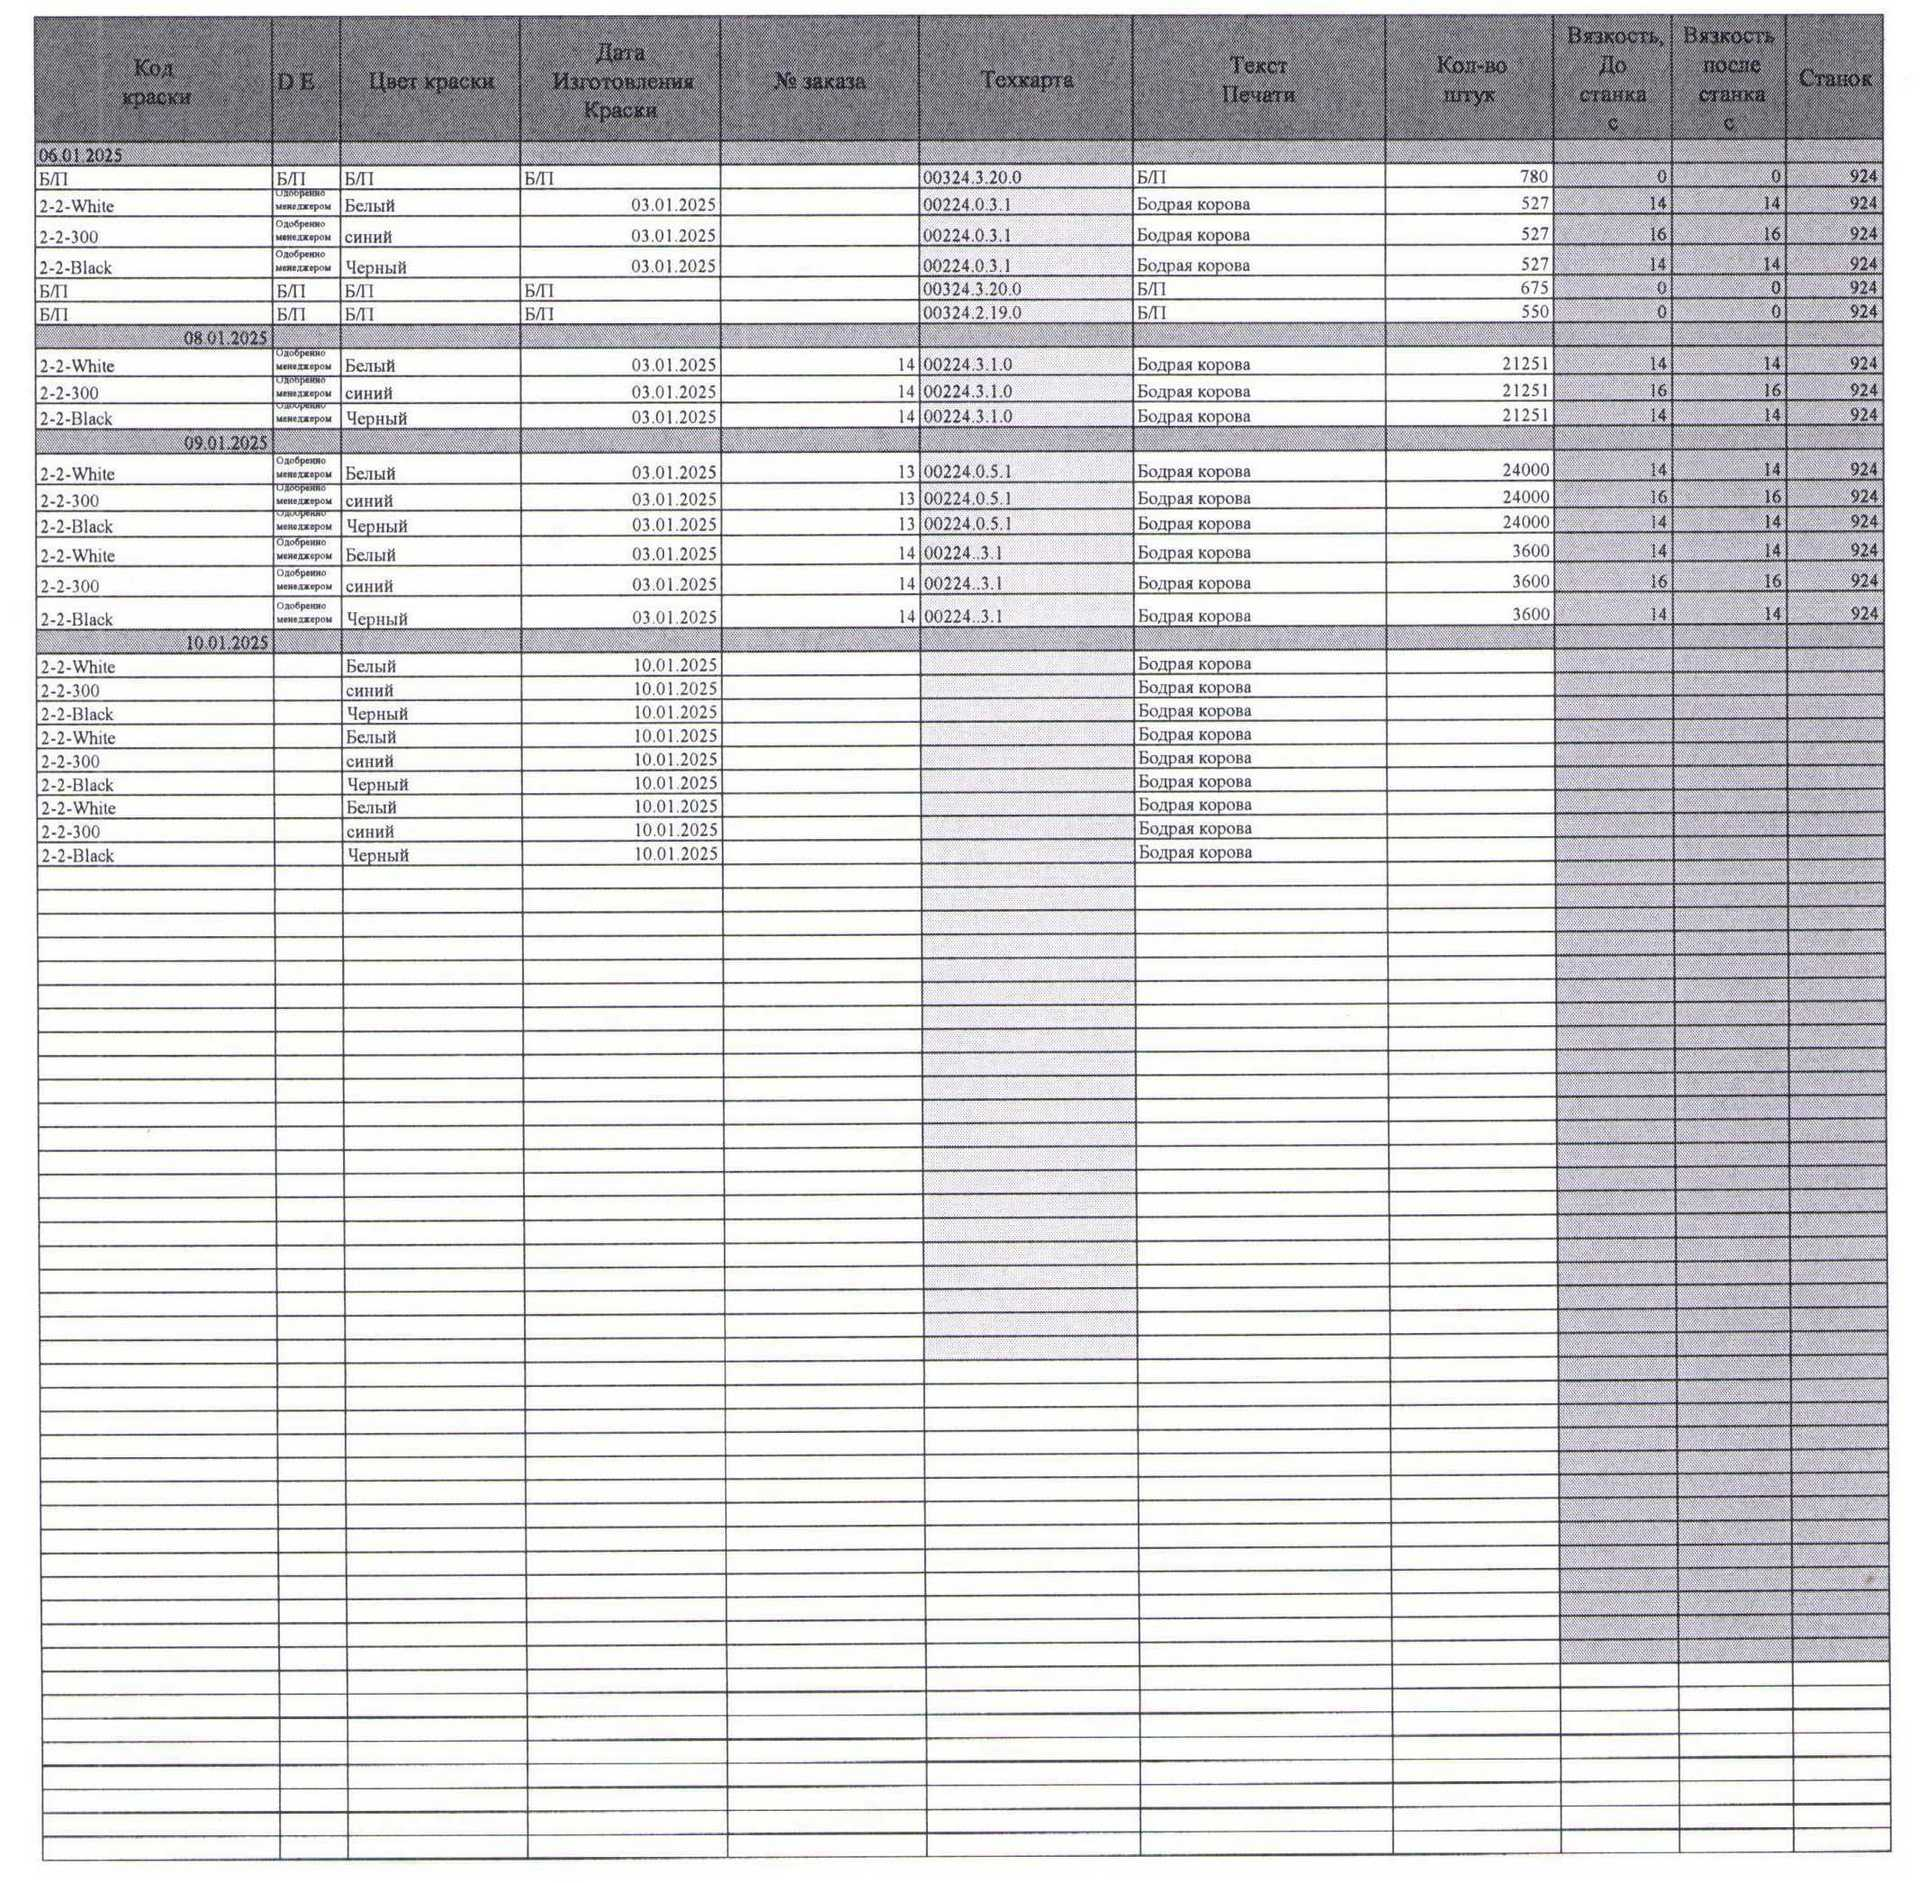
\includegraphics[width=\linewidth, height=0.94\textheight, angle=90, keepaspectratio]{Pics/f19.jpg}
\end{center}
\caption{Учет выдачи готовой краски на производство. Часть 1}
\label{pic:f19}
\end{figure}

\begin{figure}
\begin{center}
 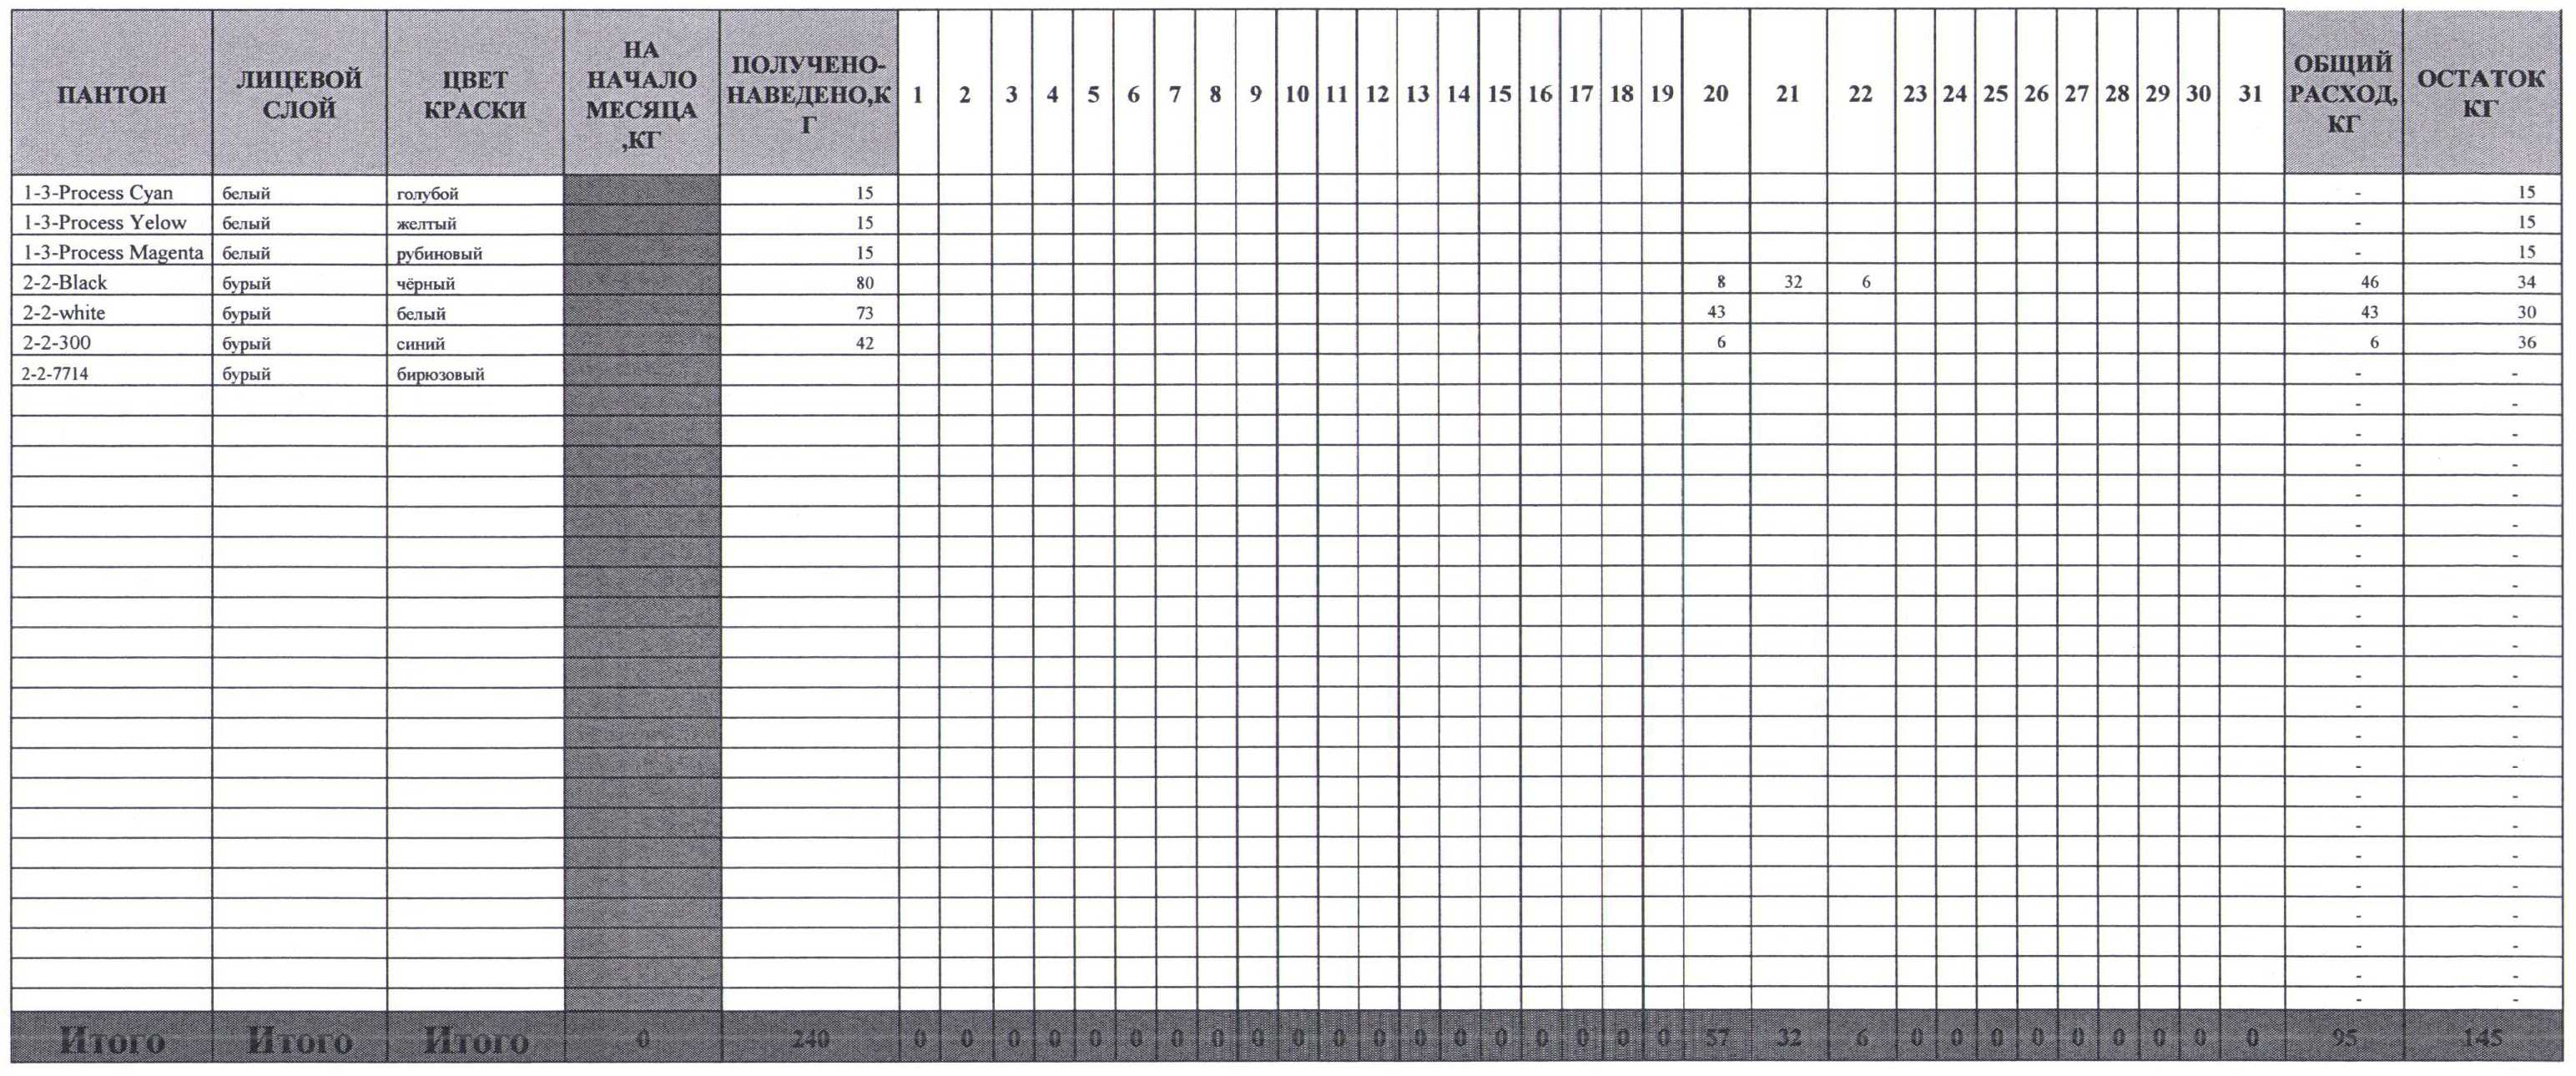
\includegraphics[width=\linewidth, height=0.94\textheight, angle=90, keepaspectratio]{Pics/f20.jpg}
\end{center}
\caption{Учет выдачи готовой краски на производство. Часть 2}
\label{pic:f20}
\end{figure}

\begin{figure}
\begin{center}
 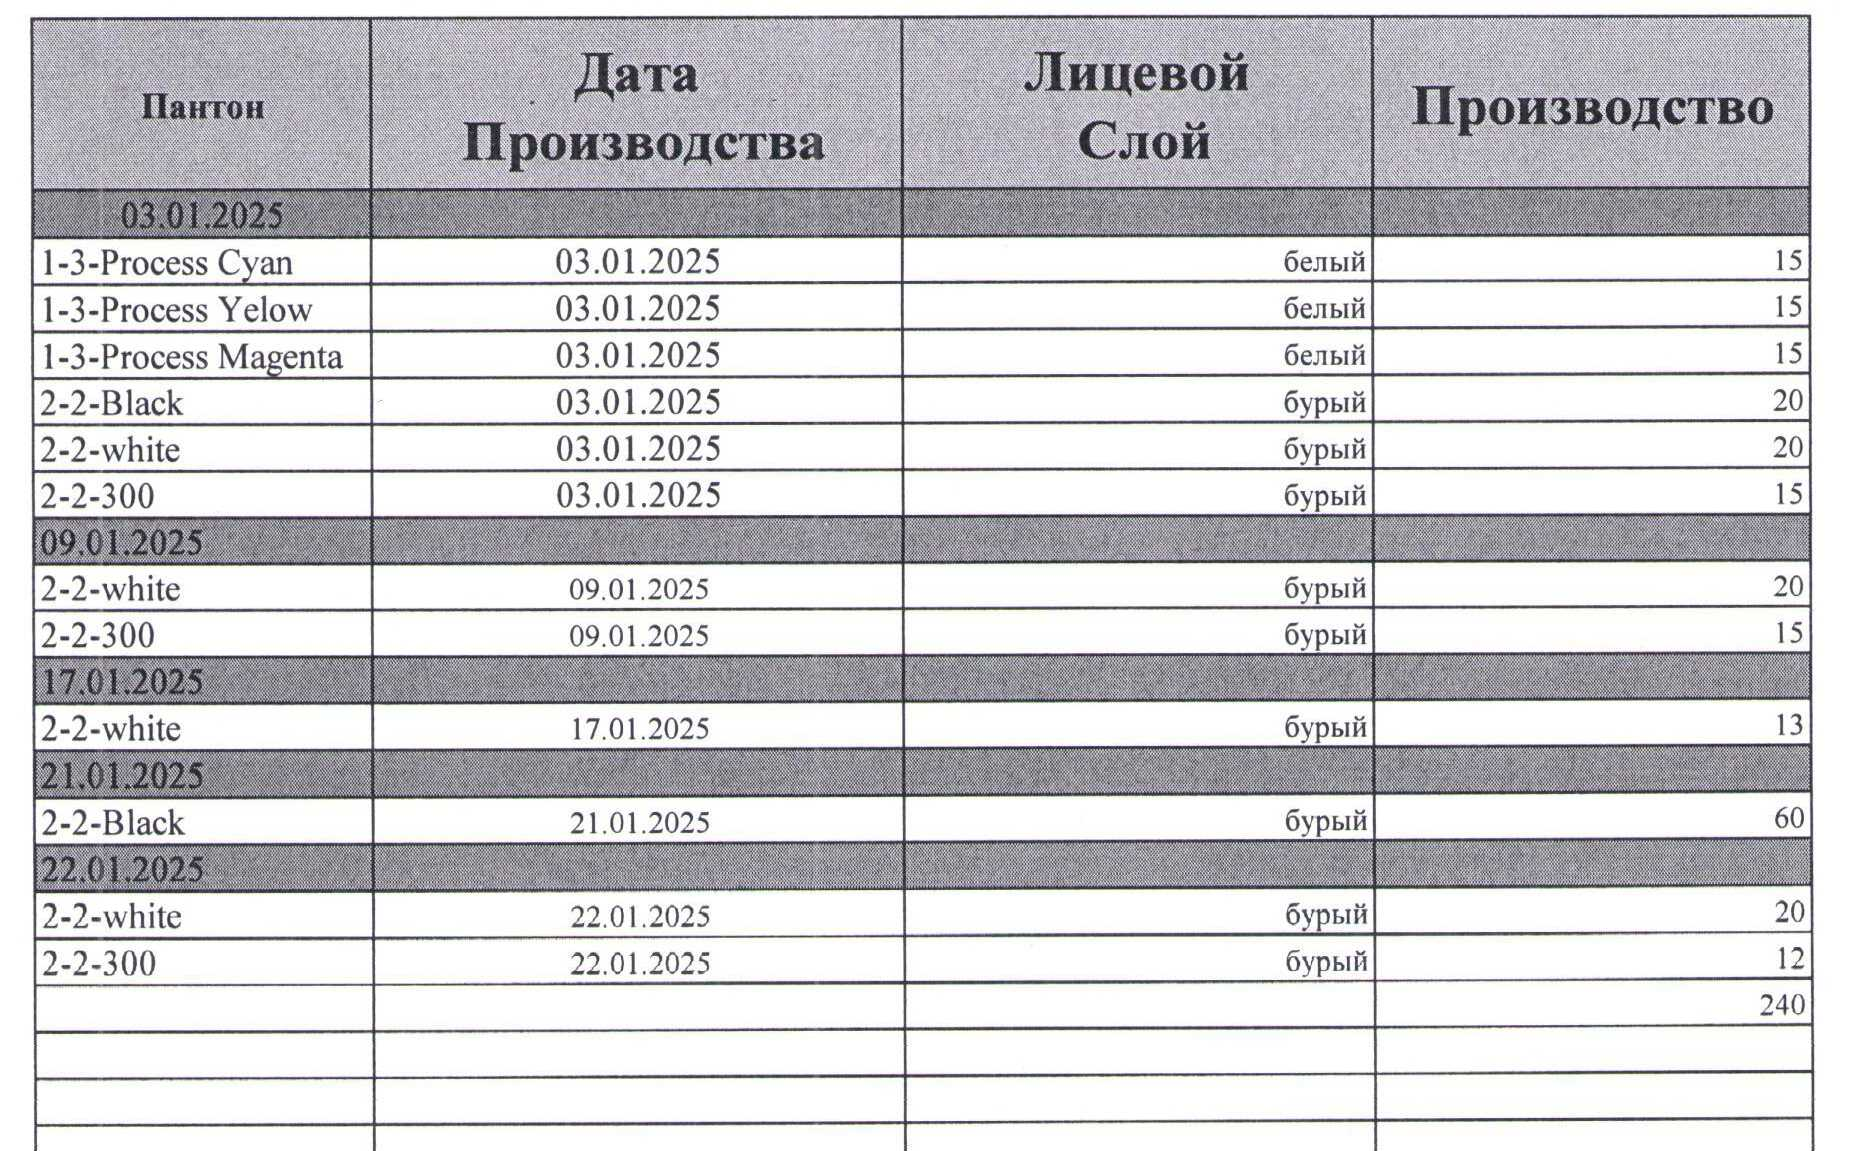
\includegraphics[width=\linewidth, height=0.94\textheight, keepaspectratio]{Pics/f21.jpg}
\end{center}
\caption{Баланс по краске}
\label{pic:f21}
\end{figure}




\clearpage
\ifx \notincludehead\undefined
\normalsize
\end{document}
\fi
 % Учет технологической оснастки и краски
% \clearpage
% \ifx \notincludehead\undefined
\normalsize
\end{document}
\fi


\newpage
\subsection{Управление и диспетчеризация производства}
\label{bp:production}

% На производстве работает 16 машинистов, 2 погрузчика (водителя), 1 грузчик, 1 инженер технолог, 1 инженер качества, 1 комплектовщик оснастки, 1 мастер смены.


Производство работает в одну смену. 





\textbf{Выработка гофроагрегата}


Мастер смены выдает задание на ГА (рис. \ref{pic:f29}). Машинист вбивает данные на продольной и поперечной резках в систему управления заказами на гофроагрегате Hsieh Hsu.

Бригадир передает в устной форме на склад запрос на поставку необходимого сырья, предварительно посмотрев <<домоты>> (остатки по рулонам). Бригадир совместно с кладовщиком заполняют ведомость по сырью (рис. \ref{pic:f26}). Переданный на производство со склада рулон сразу списывается с учета.


Машинисты запускают ГА, производят гофрокартон согласно  планового задания. 

Данные по выработке вносят в MS EXCEL (рис. \ref{pic:f23}).

Бирки на полуфабрикаты, выпущенные на ГА, машинисты печатают (рис. \ref{pic:f31}) сразу на весь заказ. Бирки печатаются непосредственно на ГА. Механизм автоматического формирования бирок не настроен.

По факту выработки с гофроагрегата машинист формирует отчет по выработке по форме (рис. \ref{pic:d6}).




\textbf{Выработка линии переработки}

Мастер смены выдает машинистам задания по линиям (рис. \ref{pic:f24}). Технологические карты бригадиры печатают с сервера. 
Краску, при возникновении необходимости, выдает колорист.
Оснастку машинисты берут сами. Оснастка хранится около производственных линий.
Машинисты настраивают машину и выпускают продукцию согласно требованиям ТК.


Бирки на готовую продукцию печатает мастер сразу на весь заказ и с плановым заданием передает на линию (рис. \ref{pic:f30}).

Выработку машинисты на линиях вносят в файл MS EXCEL  (рис. \ref{pic:f23}).


Бригадиры на перерабатывающих линиях ведут таблицу MS EXCEL с указанием простоев (рис. \ref{pic:f28}. Подробнее процесс описан в разделе \ref{bp:maintance}).

В конце смены на основании данных по выработкам из таблицы MS EXCEL мастер заполняет отчет производства за смену (рис. \ref{pic:f25}).

Также мастер заполняет ведомость передачи ГП на склад и сверяется с данными кладовщика готовой продукции (рис. \ref{pic:f6}).




\begin{figure}
\begin{center}
 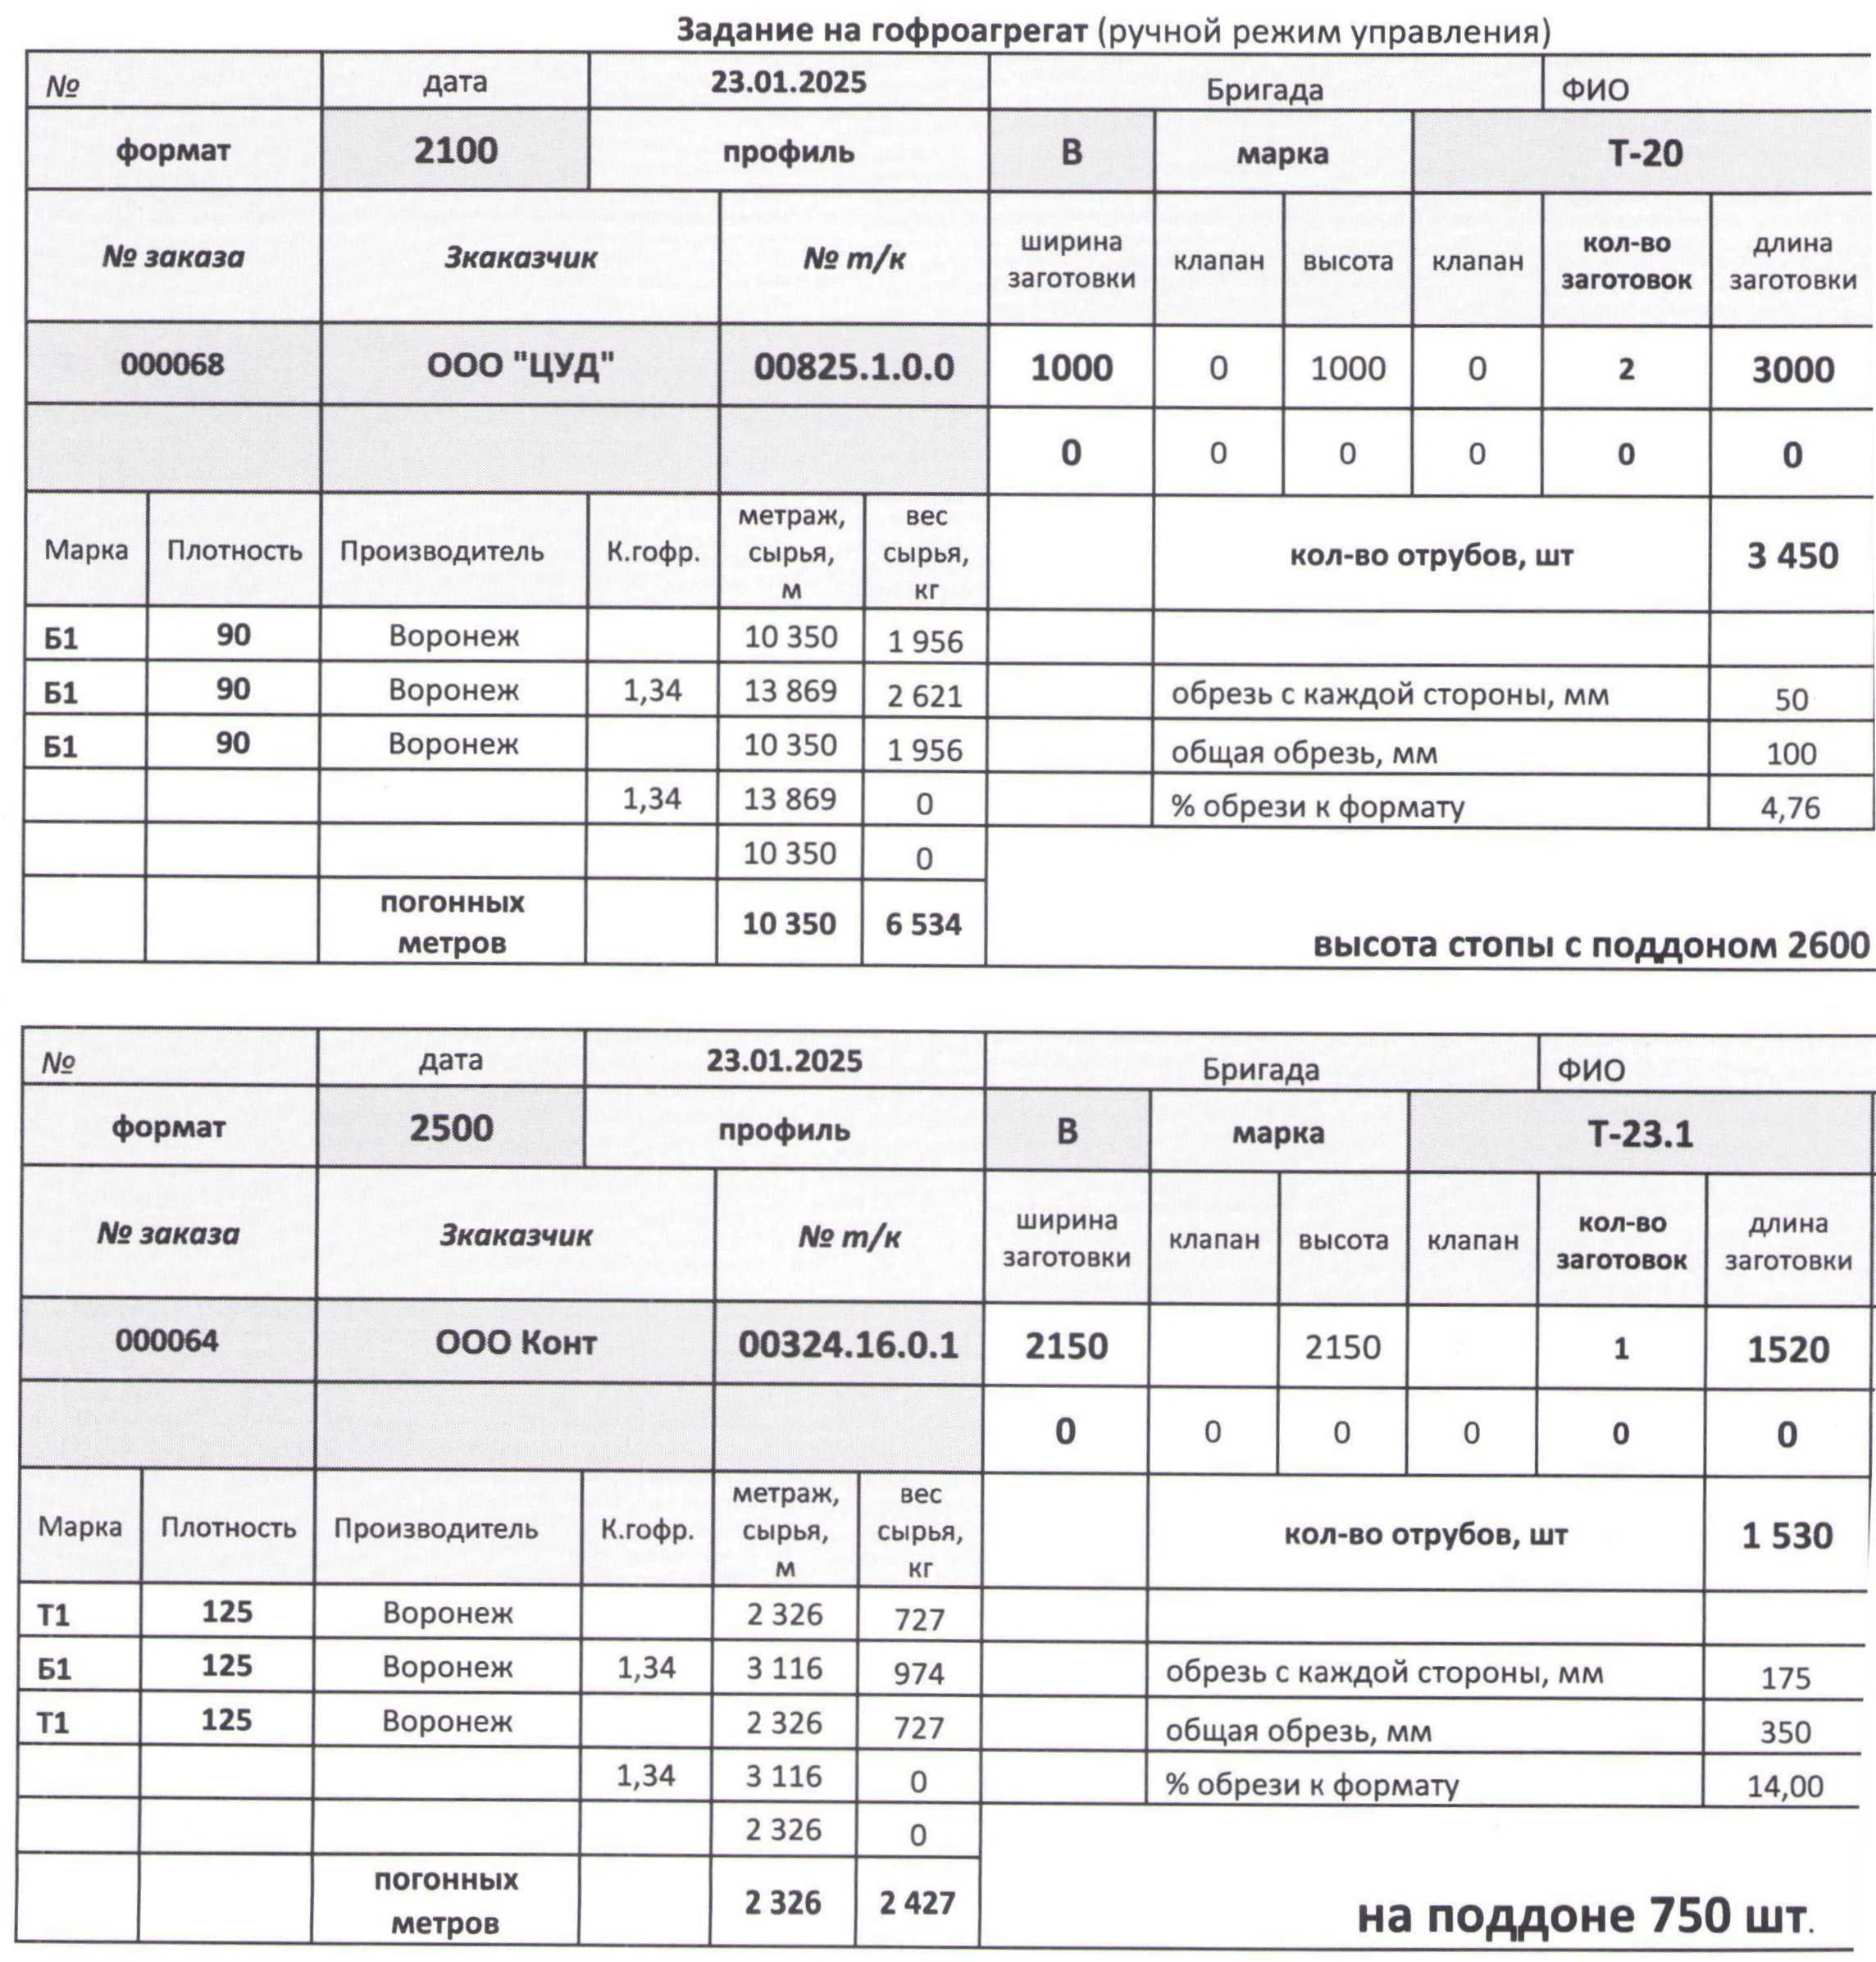
\includegraphics[width=\linewidth, height=0.94\textheight, keepaspectratio]{Pics/f29.jpg}
\end{center}
\caption{Задание на смену для ГА}
\label{pic:f29}
\end{figure}

\begin{figure}
\begin{center}
 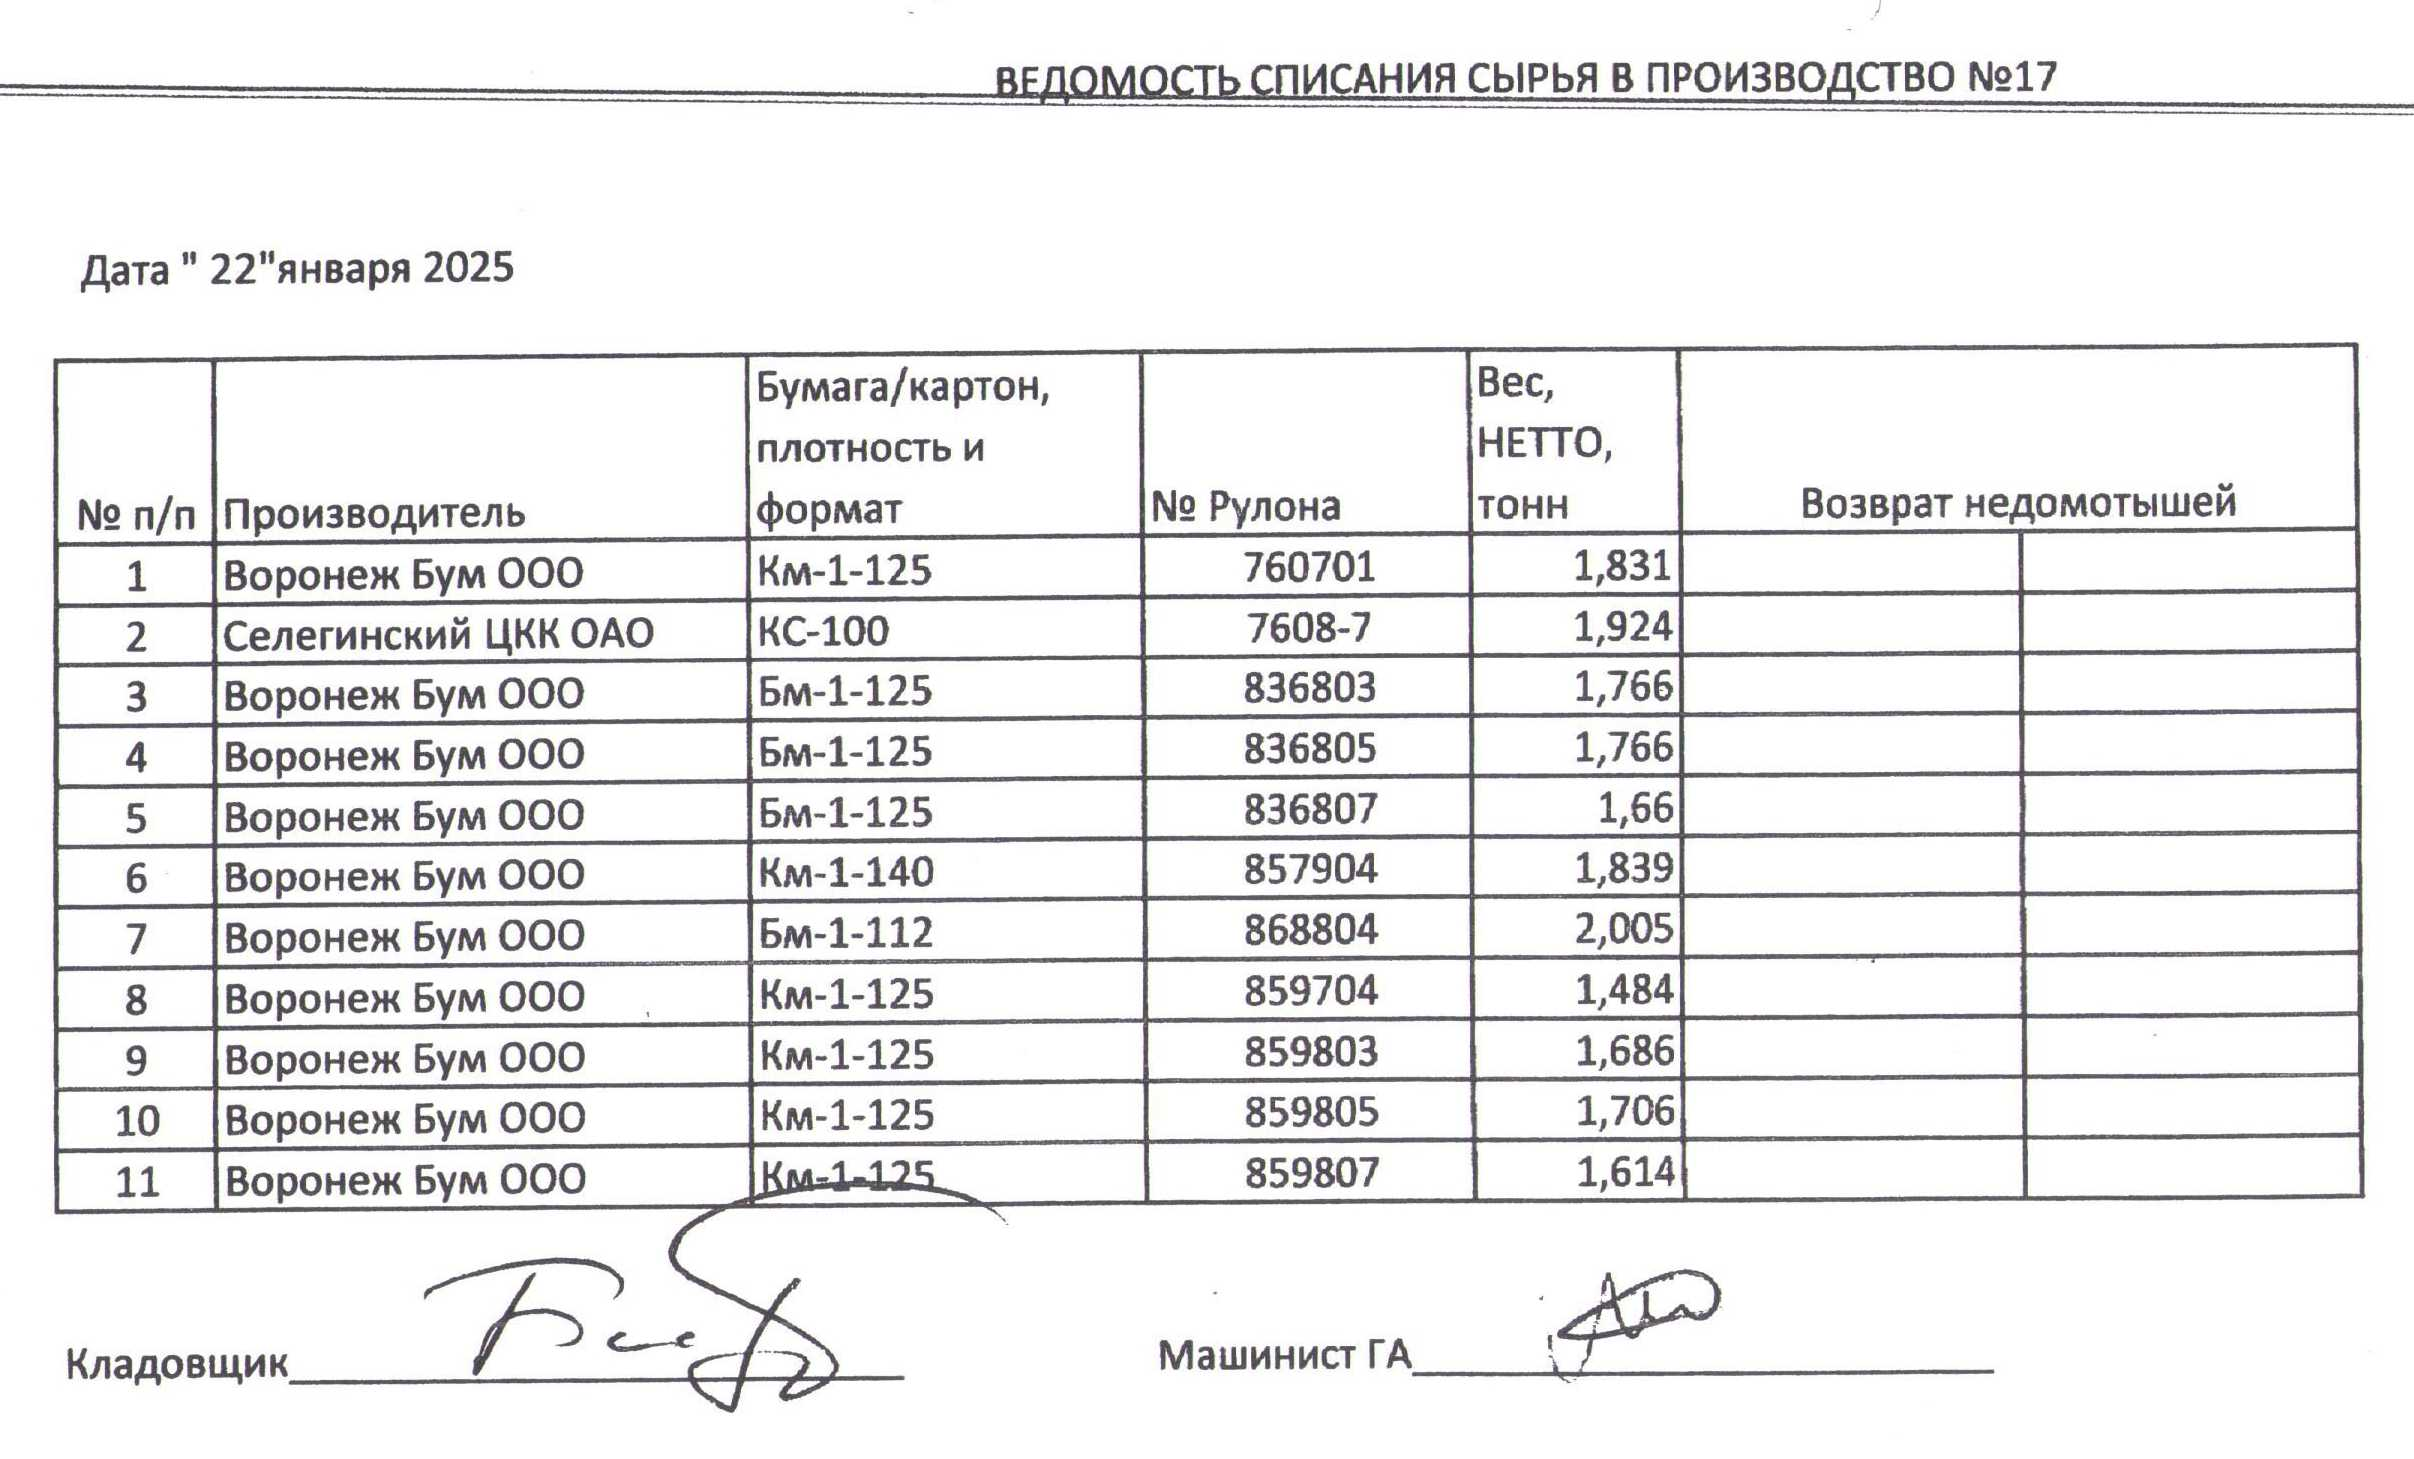
\includegraphics[width=\linewidth, height=0.94\textheight, keepaspectratio]{Pics/f26.jpg}
\end{center}
\caption{Ведомость по сырью}
\label{pic:f26}
\end{figure}

\begin{figure}
\begin{center}
 \includegraphics[width=\linewidth, height=0.94\textheight, keepaspectratio]{Pics/f23.jpg}
\end{center}
\caption{Учет выработки}
\label{pic:f23}
\end{figure}

\begin{figure}
\begin{center}
 \includegraphics[width=\linewidth, height=0.94\textheight, keepaspectratio]{Pics/f31.jpg}
\end{center}
\caption{Бирки на ПФ}
\label{pic:f31}
\end{figure}

\begin{figure}
\begin{center}
 \includegraphics[width=\linewidth, height=0.94\textheight, keepaspectratio]{Pics/d6.jpg}
\end{center}
\caption{Отчет производства за смену ГА}
\label{pic:d6}
\end{figure}

\begin{figure}
\begin{center}
 \includegraphics[width=\linewidth, height=0.94\textheight, keepaspectratio]{Pics/f24.jpg}
\end{center}
\caption{Задание на смену для ПЛ}
\label{pic:f24}
\end{figure}

\begin{figure}
\begin{center}
 \includegraphics[width=\linewidth, height=0.94\textheight, keepaspectratio]{Pics/f30.jpg}
\end{center}
\caption{Бирки на ГП}
\label{pic:f30}
\end{figure}

\begin{figure}
\begin{center}
\includegraphics[height=0.94\textheight, width=\textwidth, angle=90, keepaspectratio]{Pics/f28.jpg}
\end{center}
\caption{Журнал простоев и неисправностей}
\label{pic:f28}
\end{figure}

\begin{figure}
\begin{center}
 \includegraphics[width=\linewidth, height=0.94\textheight, keepaspectratio]{Pics/f25.jpg}
\end{center}
\caption{Отчет производства за смену ПЛ}
\label{pic:f25}
\end{figure}

\begin{figure}
\begin{center}
 \includegraphics[width=\linewidth, height=0.94\textheight, keepaspectratio]{Pics/f6.jpg}
\end{center}
\caption{Ведомость передачи ГП на склад}
\label{pic:f6}
\end{figure}

\clearpage % Управление и диспетчеризация производства
% % \newpage
\subsection{Изготовление образцов продукции}
\label{bp:pattern}


Процедуры изготовления образцов не выявлено. На момент обследования строилось помещение для плоттера для изготовления образцов. 



\ifx \notincludehead\undefined
\normalsize
\end{document}
\fi % Изготовление образцов продукции
% % \newpage
\subsection{Запуск опытной партии}
%

На момент проведения аудита процесс не определен.




\ifx \notincludehead\undefined
\normalsize
\end{document}
\fi
 % Запуск опытной партии
% % \newpage
\subsection{Учет отходов производства (макулатуры)}

 

Вся макулатура в виде отходов производства передается в пресс. Прессовщик тюки с  макулатурой складывает в отдельно отведенном месте. Тюки не взвешиваются, на момент обследования не было весов. 

Кладовщик каждый день ведет учет в штуках (тюках).




%\textbf{Учет брака}




\clearpage
\ifx \notincludehead\undefined
\normalsize
\end{document}
\fi % Учет отходов производства (макулатуры)
% \newpage
\subsection{Учет готовой продукции}
\label{bp:readygoods}


Вся готовая продукция поступает на линию упаковки. Водитель погрузчика забирает паллеты с упакованной готовой продукцией на склад ГП. 

На складе ГП есть разметка для ячеечного хранения продукции (рис. \ref{pic:f5}).

Водитель погрузчика расставляет продукцию на складе в свободные ячейки и указывает в ведомости параметры продукции и ячейку, куда поставил ГП (рис. \ref{pic:f7}). В конце смены ведомость передается кладовщику. Кладовщик вносит данные в таблицу MS EXCEL (рис. \ref{pic:f10}).

В конце смены мастер смены заполняет свою ведомость по данным работы производственной  линий (рис. \ref{pic:f6}). По этой ведомости мастер сверяется с данными подаваемыми кладовщиком и подтверждают факт подписями. 


\begin{figure}
\begin{center}
\includegraphics[height=0.94\textheight, width=\textwidth, keepaspectratio]{Pics/f5.jpg}
\end{center}
\caption{Склад ГП. Разметка предусматривающая ячеистое хранение продукции}
\label{pic:f5}
\end{figure}


\begin{figure}
\begin{center}
\includegraphics[height=0.94\textheight, width=\textwidth, keepaspectratio]{Pics/f7.jpg}
\end{center}
\caption{Ведомость карщика склада ГП}
\label{pic:f7}
\end{figure}

 % Учет готовой продукции
% \newpage
\subsection{Поступление материалов}
\label{bp:MatInput}
%


\subsubsection{Поступление бумаги и картона}

Рулоны бумаги и картона принимаются кладовщиками на склад ролевой продукции. 

Сырье транспортируется машинами. При срочной необходимости могут с предприятия <<Эколайнер>>  привезти автопогрузчиком необходимый рулон. 

Сырье с <<Эколайнер>> поступает по актам передачи (рис. \ref{pic:f13}). Их подписывают кладовщики. Сырье других поставщиков приходит с обычным пакетом документов. 

При поступлении сырья на склад кладовщик сверяет данные, указанные на маркировочных этикетках рулонов с сырьем, с данными, указанными в документах (рис. \ref{pic:f9}), вносит данные в таблицу MS EXCEL (рис. \ref{pic:f1}), где ведется основной учет. 

Основные документы сразу поступают в бухгалтерию.





% \subsubsection{Поступление рулонов бумаги и картона}

% Не производится.




\subsubsection{Поступление прочих материалов}

На момент обследования все вспомогательные материалы числятся на складе другого завода.



\begin{figure}
\begin{center}
\includegraphics[height=0.94\textheight, width=\textwidth, keepaspectratio]{Pics/f13.jpg}
\end{center}
\caption{Акт на передачу}
\label{pic:f13}
\end{figure}

\begin{figure}
\begin{center}
\includegraphics[height=0.94\textheight, width=\textwidth, angle=90, keepaspectratio]{Pics/f1.jpg}
\end{center}
\caption{По рулонный учет сырья}
\label{pic:f1}
\end{figure}

\begin{figure}
\begin{center}
\includegraphics[height=0.94\textheight, width=\textwidth, angle=90, keepaspectratio]{Pics/f9.jpg}
\end{center}
\caption{Отвес сырья}
\label{pic:f9}
\end{figure}


\clearpage
\ifx \notincludehead\undefined
\normalsize
\end{document}
\fi % Поступление материалов
% \newpage
%
\subsection{Списание материалов}
\label{bp:MatOutput}

\subsubsection{Списание бумаги и картона}


Бригадир ГА получает плановое задание на гофроагрегат (рис. \ref{pic:f8b} - \ref{pic:f8a}),
определяет потребность в сырье, в устной форме передает ее кладовщику. Кладовщик с водителем погрузчика находят необходимое сырье и подают на гофроагрегат.

Сырьевые остатки в виде частично использованных рулонов обратно на склад не возвращаются. Учет частично использованных рулонов ведется производством в штуках, а не в килограммах (отсутствуют весы).

Все переданное на производство сырье кладовщик вносит в таблицу MS EXCEL с указанием даты передачи.

Кладовщик ведет ведомость списания сырья, которую подписывает бригадир, и передает ее в бухгалтерию (рис. \ref{pic:f26}).

Все остатки формируются ежедневно в таблице MS EXCEL (рис. \ref{pic:f2}).

На складе сырья планируется выполнить разметку для ячеечного хранения продукции (рис. \ref{pic:f4}). 




\subsection{Учет вспомогательных материалов}

Каждый день кладовщик сверяет остатки ТМЦ на складе с данными таблицы MS EXCEL (рис. \ref{pic:f2}) и вносит необходимые корректировки.

Деревянные поддоны учитываются отдельно и выдаются на производство по ведомости  (рис. \ref{pic:f27}).





\begin{figure}
\begin{center}
\includegraphics[height=0.94\textheight, width=\textwidth, keepaspectratio]{Pics/f8b.jpg}
\end{center}
\caption{Задание на ГА. Часть 1}
\label{pic:f8b}
\end{figure}

\begin{figure}
\begin{center}
\includegraphics[height=0.94\textheight, width=\textwidth, keepaspectratio]{Pics/f8a.jpg}
\end{center}
\caption{Задание на ГА. Часть 2}
\label{pic:f8a}
\end{figure}

\begin{figure}
\begin{center}
\includegraphics[height=0.94\textheight, width=\textwidth, angle=90, keepaspectratio]{Pics/f4.jpg}
\end{center}
\caption{Склад сырья. Разметка предусматривающая ячеистое хранение продукции}
\label{pic:f4}
\end{figure}

\begin{figure}
\begin{center}
\includegraphics[height=0.94\textheight, width=\textwidth, keepaspectratio]{Pics/f2.jpg}
\end{center}
\caption{Остатки ТМЦ}
\label{pic:f2}
\end{figure}

\begin{figure}
\begin{center}
\includegraphics[height=0.94\textheight, width=\textwidth, keepaspectratio]{Pics/f27.jpg}
\end{center}
\caption{Ведомость списания вспомогательных материалов в производство}
\label{pic:f27}
\end{figure}

\clearpage
\ifx \notincludehead\undefined
\normalsize
\end{document}
\fi % Списание материалов
% % \newpage
%
\subsection{Инвентаризация материалов}
%\label{bp:MatOutput}

На момент обследования инвентаризация не проводилась.

% \clearpage
\ifx \notincludehead\undefined
\normalsize
\end{document}
\fi % Инвентаризация материалов
% % \newpage
\subsection{Управление качеством}
\label{bp:quality}
%\subsection{Управление качеством}

На предприятии создана лаборатория.  Закуплено оборудование. На момент проведения аудита измерения показателей качества не проводились.
%\textcolor{red}{Тут наверное нужно указать введена ли лаборатория в эксплуатацию или находится на стадии оснащения или подбора персонала?}



\clearpage
\ifx \notincludehead\undefined
\normalsize
\end{document}
\fi % Управление качеством
% % \newpage
\subsection{Претензии контрагентов}
\label{BP_CLaim} 

Процедуры регистрации претензии контрагентов не выявлено. 
Процесс не определен.


\clearpage
\ifx \notincludehead\undefined
\normalsize
\end{document}
\fi % Претензии контрагентов
% % \newpage
\subsection{Ремонты и ППР}
\label{bp:maintance}


На предприятии создана служба ремонта. 

При поломке оборудования бригадир информирует мастера смены. Мастер смены вызывает необходимого специалиста. Простои фиксирует мастер смены у себя в рапорте. 

Ведется таблица MS EXCEL по поломкам и неисправностям. Машинисты вносят в нее замечания. Служба ремонта вписывает комментарии и сроки устранения (рис. \ref{pic:f28}).




 % Ремонты и ППР
% % \newpage
\subsection{Управление закупками}
% %\todo{ÏÈÑÀÒÜ}

 Менеджер по закупкам смотрит остатки ТМЦ в MS EXCEL (рис. \ref{pic:f2}) и, при возникновении необходимости, заказывает необходимые материалы.
% %
% \clearpage
% \ifx \notincludehead\undefined
\normalsize
\end{document}
\fi


 % Управление закупками
% % \newpage
\subsection{Управление персоналом}
%\todo{ÏÈÑÀÒÜ}
%
Для автоматизации функций управления персоналом используется программный продукт 1С:ЗУП.
 % Управление персоналом
% % \newpage
\subsection{Расчет заработной платы}
%\todo{ÏÈÑÀÒÜ}

% Бригадир ведет табели учета рабочего времени (рис. \ref{pic:f44}).


Для расчета ЗП и автоматизации функций управления персоналом используется программный продукт 1С:ЗУП.


 % Расчет заработной платы
% % \newpage
\subsection{Ведение бухгалтерского учета}
%\todo{ÏÈÑÀÒÜ}
% %
Для первичного управленческого учета внедряется система «1С:Управление нашей фирмой».

Для ведения бухгалтерского и налогового учета используется система 1С:Бухгалтерия 8.
 % Ведение бухгалтерского учета
% % \newpage
\subsection{Расчет фактической себестоимости продукции}
%\todo{ÏÈÑÀÒÜ}
% %
Фактическая себестоимость рассчитывается главным бухгалтером котловым методом на весь выпуск продукции в системе 1С:Бухгалтерия 8. 

Учет незавершенного производства на момент аудита не ведется.

 % Расчет фактической себестоимости продукции




%%%%%%%%%%%%%%%%%%%%%%%%%%%%%%%%%%%%%%%%%%%%%%%%%%%%%%%%%%%%%%%%%%%%%%%%%%%%%%%%%%%%%%%%%%%%%%%%%%%%%%%%%


%
\newpage
\section{Предлагаемая схема информационных потоков в БП}

\subsection{Процессы ''Подготовка производства'', ''Учет технологической оснастки''}
%%
\begin{figure}
\begin{center}
  \includegraphics[angle=90, height=0.9\textheight, keepaspectratio]{Pics/1_NewGoods.pdf}
\end{center}
  \caption{Процессы ''Подготовка производства'', ''Учет технологической оснастки''}
  \label{pic:Schema_1}
\end{figure}
\clearpage

При появлении нового контрагента менеджер будет создавать в справочнике ''Контрагенты'' новый элемент справочника в системе Opti-Corrugated (Опти-Софт) для покупателей и в системе 1С:УНФ для других контрагентов (см. рис. \ref{pic:Schema_1}).


При автоматическом обмене 1С:УНФ выгрузит новый элемент ''Контрагенты'' в систему  Опти-Софт (СИСТЕМА). При обмене справочники ''Контрагенты'' будут синхронизированы. 

Менеджер при появлении требований от заказчика рассчитывает цену продажи изделия в таблице MS EXCEL. После согласования цены при необходимости менеджер создает автоматически номенклатуру нового изделия в справочнике ''Номенклатура'' в СИСТЕМЕ. 

При автоматическом обмене система 1С:УНФ выгрузит новый элемент ''Номенклатура'' в систему Опти-Софт и загрузит новые обратно. При обмене справочники ''Номенклатура'' будут синхронизированы. 

% На основании выполненного расчета цены менеджер формирует печатную форму коммерческого предложения и высылает клиенту. %Есть возможность выслать предложение прямо из СИСТЕМЫ.
% Менеджер будет формировать печатную форму договора и спецификации цены из системы 1С:УНФ. 

После согласования цены менеджер создает в СИСТЕМЕ документ ''Заявка-спецификация'' -- распоряжение технологу по разработке оснастки и технологической карты. 

Отдел главного технолога создает технологическую карту в СИСТЕМЕ, которую менеджер должен согласовать в печатном виде с заказчиком. 



\subsection{Процессы ''Управление продажами''}
%%
\begin{figure}
\begin{center}
  \includegraphics[angle=90, height=0.9\textheight, keepaspectratio]{Pics/2_Sales.pdf}
\end{center}
  \caption{Процессы ''Управление продажами''}
  \label{pic:Schema_2}
\end{figure}
\clearpage
% %
% Модуль CRM будет работать в системе 1С:УНФ.




После согласования технологической карты менеджер может создать в СИСТЕМЕ заявку покупателя. При создании заявки покупателя СИСТЕМА проверяет остатки по готовой продукции на складе по данным  складского учета в СИСТЕМЕ. Остатки будут определяться автоматически по оперативным данным (см. рис. \ref{pic:Schema_2}).
% %, автоматически проверяет задолженность по покупателю на основе данных программы 1С: Бухгалтерия. 

% %В документе ''Заявка'' менеджер должен выбрать организацию внутреннюю. 
% %Менеджер при необходимости будет выполнять расчет предварительной загрузки транспорта.


Менеджер выполняет в СИСТЕМЕ предварительное планирование, при котором СИСТЕМА подскажет возможную дату выполнения производственного заказа. 
Менеджер  утверждает плановую дату производства для позиций заявки.

После согласования условий с клиентом для запуска заявки в производство менеджер должен поменять статус заявки на "Одобрено к выпуску". После согласования даты менеджер создает производственный заказ. После изменения статуса заказы видны в СИСТЕМЕ в отделе планирования. 
   
% %\newpage
% %%
\subsection{Процессы ''Предварительное планирование'', ''Оперативное планирование''}
%
\begin{figure}
\begin{center}
  \includegraphics[angle=90, height=0.8\textheight, keepaspectratio]{Pics/3_Plan.pdf}
\end{center}
  \caption{Процессы ''Предварительное планирование'', ''Оперативное планирование''}
  \label{pic:Schema_3}
\end{figure}
\clearpage


Из отдела продаж заказы с одобренным статусом появляются в СИСТЕМЕ у планировщика.

Планировщик выполняет оперативное планирование работы гофроагрегата и линий переработки. По факту планирования работы гофроагрегата, Планировщик в СИСТЕМЕ формирует потребности по материалам, создает документ ''Заказ поставщику''. 
В результате Планировщик формирует оперативный план работы по гофроагрегату и линиям переработки.
План производства доступен на производстве для выполнения.



% По регламенту СИСТЕМА выгружает все складские документы в систему 1С:УНФ.
% %
% %\newpage
% %%
\subsection{Процессы ''Управление производством''}
%
\begin{figure}
\begin{center}
  \includegraphics[angle=90, height=0.9\textheight, keepaspectratio]{Pics/4_Output.pdf}
\end{center}
  \caption{Процессы ''Управление производством''}
  \label{pic:Schema_4}
\end{figure}
% \clearpage




 Машинист гофроагрегата получает оперативный план производства на своем рабочем месте в СИСТЕМЕ. Машинист гофроагрегата должен в СИСТЕМЕ зафиксировать выработку по гофроагрегату (в документе ''Выработка гофроагрегата''), в т.ч. брак в работе гофроагрегата, простои и неисправности.

Рабочее место машиниста будет подключено к гофроагрегату Hsien Hsu. По команде машиниста раскрои будут выгружаться автоматически в память гофроагрегата.
После выполнения раскроя данные по выработке будут загружены в рабочее место в СИСТЕМУ.

Машинист на технологической линии получает оперативный план производства линии на своем рабочем месте в СИСТЕМЕ. Машинист технологической линии фиксирует факт выработки по заказу, отклонения, в т.ч. брак при работе линии, простои и неисправности (см. рис. \ref{pic:Schema_4}).

% Документы по выработке ''Выработка гофроагрегата'', ''Выработка по переработке'' при автоматическом обмене СИСТЕМА выгрузит в документы ''Отчет производства'' в систему 1С:УНФ.



\subsection{Процессы ''Планирование отгрузки'', ''Управление качеством'', ''Управление продажами''}
%
\begin{figure}
\begin{center}
  \includegraphics[angle=90, height=0.9\textheight, keepaspectratio]{Pics/5_Shipment.pdf}
\end{center}
  \caption{Процессы ''Планирование отгрузки'', ''Управление качеством'', ''Управление продажами''}
  \label{pic:Schema_5}
\end{figure}
% \clearpage



Цена продукции по умолчанию будет указана в справочнике ''Номенклатура'' менеджером.


По факту изготовления готовой продукции менеджер будет контролировать в СИСТЕМЕ состояние заказа, его готовность и местоположение.
При готовности заказа менеджер будет создавать в СИСТЕМЕ документ ''Заявка на отгрузку'' либо вручную, либо на основании заявки покупателя.
Логист отдела продаж в СИСТЕМЕ указывает в документах ''Заявка на отгрузку'' транспорт, который будет подан под погрузку. Логист планирует транспорт под погрузку.

Логист планирует размещение груза в транспортном средстве в СИСТЕМЕ через оптимизатор погрузки.

Заявка на отгрузку будет автоматически или по запросу выгружена из СИСТЕМЫ в систему 1С:УНФ в документ "ЗаявкаНаОтгрузку".

Отгрузка готовой продукции будет выполняться в СИСТЕМЕ кладовщиком на основании документа ''ЗаявкаНаОтгрузку'' (см. рис. \ref{pic:Schema_5}).

% Кладовщик на производстве будет видеть в системе 1С:УНФ все распоряжения на отгрузку (Заявка на отгрузку).
% При поступлении транспорта кладовщик создает на основании документа ''Распоряжение на отгрузку'' документ ''Реализация ТМЦ''. По факту отгрузки кладовщик корректирует при необходимости факт отгрузки в документе ''Реализация ТМЦ''. 

Кладовщик печатает сопроводительные документы в системе 1С:УНФ: ТН, ТТН.
Бухгалтер печатает сопроводительные документы в системе 1С:УНФ: счет-фактура, расходная накладная.

% Документы ''Реализация ТМЦ''  при автоматическом обмене СИСТЕМА выгрузит в документы ''Реализация'' в систему 1С:УНФ.


% %
% %
\subsection{Процессы ''Поступление материалов'', ''Списание материалов в производство''}
%
\begin{figure}
\begin{center}
  \includegraphics[angle=90, height=0.8\textheight, keepaspectratio]{Pics/6_Warehouse.pdf}
\end{center}
  \caption{Процессы ''Поступление материалов'', ''Списание материалов в производство''}
  \label{pic:Schema_6}
\end{figure}
% \clearpage

% Учет материалов остается в системе 1С:УНФ как есть.

Материалы (заготовки) будет оприходовать мастер производства в системе Опти-Софт документом ''Поступление ТМЦ''. Рулоны бумаги и картона оприходует кладовщик 
в системе Опти-Софт документом ''Поступление ТМЦ''.

При необходимости перемещения рулонов на гофроагрегат кладовщик создает документ ''Перемещение ТМЦ'' в системе Опти-Софт.

% Кладовщик на производстве в СИСТЕМЕ оприходует поступающие материалы и заготовки в СИСТЕМЕ в документе "Поступление ТМЦ". 
% Мастер на производстве фиксирует перемещение ТМЦ документом "Перемещение ТМЦ".

% Операторы на раскатах фиксируют сырье, использованное при производстве гофрокартона, в документе "Сырье для выработки".
% Кладовщик выполняет списание в производство  в СИСТЕМЕ документом ''Списание ТМЦ'' на основании документа "Сырье для выработки".

Документы автоматически выгружаются в систему 1С:УНФ по регламенту (см. рис. \ref{pic:Schema_6}).

%
%
%
%
%
%%
%%\newpage
%%
%%\subsection{Процессы 'Управление и диспетчеризация производства', 'Списание бумаги и картона', 'Управление качеством', 'Учет готовой продукции', 'Планирование отгрузки', 'Отгрузка готовой продукции'}
%%
%%\begin{figure}
%%\begin{center}
%%  \includegraphics[height=0.94\textheight, keepaspectratio]{Pics/Schema_3.jpg}
%%\end{center}
%% % \caption{Процессы 'Управление и диспетчеризация производства', 'Списание бумаги и картона', 'Управление качеством', 'Учет готовой продукции', 'Планирование отгрузки', 'Отгрузка готовой продукции'}
%%  \label{pic:Schema_3}
%%\end{figure}
%%\clearpage
% % как будет	


\end{document}
